\documentclass[a4paper,12pt]{article}
\usepackage[a4paper,margin=1in]{geometry}
\usepackage{graphicx}
\usepackage{setspace}
\usepackage{titling}
\usepackage{parskip}
\usepackage{mathptmx}
\usepackage{subcaption}
\usepackage{caption}
\usepackage[dvipsnames,svgnames,x11names]{xcolor}
\usepackage{float}
\usepackage{amsmath} 
\usepackage{enumitem}  
\usepackage{amssymb}
\usepackage{booktabs}
\usepackage[authoryear]{natbib} 
%TC:macro \href        2 0
%TC:macro \url         1 0
%TC:macro \detokenize  1 0
\usepackage[colorlinks=true, citecolor=blue, linkcolor=black, urlcolor=blue]{hyperref}

\begin{document}

\begin{titlepage}
    \centering
    % Logos in corners
    \includegraphics[width=0.4\textwidth]{Cam_logo_bw.png}\\[1.5cm]


    \vspace{1cm}

    % Title
    {\LARGE \bfseries Disentangling the Components of the Milky Way}\\[0.75cm]
    {\large \textsc{Inferring the Structure of the Milky Way in Phase-Space Using Gaussian Mixture Modelling with Extreme Deconvolution}}\\[1.5cm]


    % Author
    \vspace{0.5cm}
    \large
    \textsc{A REPORT PRESENTED}\\[0.3cm]
    \textsc{BY}\\[0.3cm]
    \textsc{RAUNAQ SINGH RAI}\\[1cm]

    % Departments
    \normalsize
    \textbf{Departments}\\[0.3cm]
    Department of Physics (Cavendish Laboratory)\\
    Institute of Astronomy\\[1cm]

    % Degree
    \textbf{Degree}\\[0.3cm]
    MPhil in Data Intensive Science\\[1cm]

    % Supervision
    \textbf{Supervision}\\[0.3cm]
    Dr Anke Arentsen\\

    % College Crest and Info
    \vfill
    \includegraphics[width=0.5\textwidth]{St_Edmunds_Logo.png}\\[0.25cm]
    29th June 2025

\end{titlepage}

\begin{abstract}

The Milky Way Galaxy is a complex system composed of multiple stellar components,
each with distinct chemical and kinematic properties. The prescence of a very-metal-poor disk
structure has been speculated, which would challenge the conventional view that the disk formed 
later from already enriched gas. By reproducing and extending the Extreme-Deconvolution 
Gaussian Mixture Model (XD-GMM) study of \citet{zhang2024existencemetalpoordiscmilky}, we 
investigate the presence of a very-metal-poor disk in the Milky Way using data catalogues from 
\citet{Andrae2023}, \citet{Li2024} and \citet{BailerJones2021}. 

In general, our results are in agreement with that of \citet{zhang2024existencemetalpoordiscmilky}: 
below \(\mathrm{[M/H]}\simeq-1.6\) we do not find evidence for a coherent,   
rotationally supported disc component. The prograde rotation signal stems from
a prograde halo with a net prograde rotation of \(v_{\phi}\simeq68\;\mathrm{km\,s^{-1}}\).  
In this regime, no component satisfies \(v_{\phi}/\sigma_{\phi}>1\); 
any thick-disc contribution in the very-metal-poor interval \(-3.0<\mathrm{[M/H]}<-1.6\) 
is therefore be negligible.

Splitting the sample by $\alpha$ abundance sharpens the timeline of disc growth.  Building 
on \citet{Vis2024} with the extreme-deconvolution framework of 
\citet{zhang2024existencemetalpoordiscmilky}, we show that a rotation-supported thick disc 
appears in the \textit{high-$\alpha$} branch at \(\mathrm{[M/H]}\gtrsim -1.6\), whereas 
\textit{low-$\alpha$} stars remain halo-dominated until a rapid spin-up at 
\(\mathrm{[M/H]}\approx -1.3\), which marks the thin-disc birth.  These metallicity–$\alpha$ 
thresholds (\(-1.6\) dex and \(-1.3\) dex) constitute hard priors for chemo-dynamical 
simulations, a clean survey filter for WEAVE, 4MOST and SDSS-V to isolate the oldest 
disc stars, and inputs for \textsc{Auriga} and \textsc{FIRE-2} zoom suites to generate 
testable JWST and Rubin-LSST predictions for disc structure in other spiral galaxies.


\end{abstract}


\newpage

% -------- FIGURES PAGE --------
\listoffigures
\newpage
% -------- TABLES PAGE --------
\listoftables
\newpage

% -------- CONTENTS PAGE --------
\tableofcontents
\newpage


\section{Introduction}

The Milky Way Galaxy, host to our solar system, is a spiral galaxy with a centre 
located approximately 150\,000\,trillion miles from Earth. 
Its formation history is complex and remains an active area of research. Being embedded 
within the Milky Way means we can study it in greater detail than any external galaxy, 
testing models of galaxy formation with high-precision observational data. One of the 
central aims of Galactic Archaeology is to reconstruct the Milky Way’s assembly by 
examining the chemical compositions and dynamical properties of its stars.

In this project, we reproduce and extend the analysis of \citet{zhang2024existencemetalpoordiscmilky}, 
who investigated a very metal-poor disc component in the Milky Way. Very metal poor 
stars, formed from an interstellar medium unpolluted by earlier generations of 
supernovae, are among the oldest relics in the Galaxy. Discovering them on disc-like 
orbits would challenge the conventional view that the disc formed later from already 
enriched gas \citep{BlandHawthorn2016}, implying instead an earlier onset of disc 
assembly. 

\subsection{Components of the Milky Way}

The Milky Way is commonly decomposed into four stellar components: a \emph{thin disc}, 
a \emph{thick disc}, a central \emph{bulge/bar}, and a roughly spherical \emph{halo} 
\citep{BlandHawthorn2016,Helmi2020}.  
The thin disc describes the majority of stars and most of the interstellar gas 
in the galaxy.  Ongoing star formation is concentrated in the “molecular–gas ring’’ where young, 
metal-rich stars trace nearly circular, co-rotating 
orbits with low velocity dispersion ($\sigma_\phi \simeq 20\;\mathrm{km\,s^{-1}}$).  
Above the mid-plane lies the thick disc: an older ($\gtrsim8$–$10\;\mathrm{Gyr}$), 
moderately metal-poor population , a scale 
height of $z_{\mathrm{scale}}\approx1\;\mathrm{kpc}$, and hotter kinematics 
($\sigma_z \simeq 40\;\mathrm{km\,s^{-1}}$) while still retaining net prograde rotation.  
Inside $R\lesssim2\;\mathrm{kpc}$, the central bulge (partly bar-shaped) hosts both 
old, metal-rich stars and a younger, actively forming component; stellar motions 
there combine bar-driven streaming with high random velocities 
($\sigma\sim100\;\mathrm{km\,s^{-1}}$).  
Encasing all of these is the stellar halo, which contributes only a few per cent 
of the total stellar mass yet includes the Galaxy’s oldest, most metal-poor stars 
($[\mathrm{Fe/H}]\lesssim-1.5$) on highly eccentric or even retrograde orbits.  
Its low density, rich substructure, and kinematics indicate an origin in the
 hierarchical accretion and tidal disruption of dwarf galaxies and globular clusters.  
The spatial distribution, chemistry, and dynamics of these four components 
supply clues to the Milky Way’s formation history and its sequence of merger events.


\subsection{Metallicity as a Cosmic Clock}

Precise ages for individual old stars are difficult to measure, so their chemical 
composition, most commonly the iron-to-hydrogen ratio $[\mathrm{Fe/H}]$, is 
used as a surrogate clock.  
Very metal-poor (VMP) stars must have formed before successive generations of Type II 
and Type Ia supernovae had substantially enriched the interstellar medium, and 
therefore have low $[\mathrm{Fe/H}]$ values.  
Metallicity is inferred spectroscopically by measuring the equivalent widths of 
metal absorption lines, particularly Fe\,\textsc{i} and the Ca\,\textsc{ii} H and 
K lines at 396.8\,nm and 393.4\,nm, respectively. After correcting for stellar 
effective temperature and surface gravity, the relative strengths of these lines 
yield elemental abundances \citep{Gray_2005}.
Large surveys (for example APOGEE, GALAH, LAMOST, and the Gaia XP spectra) now 
provide such measurements for millions of stars, enabling empirical age–metallicity 
relations that link chemistry to stellar chronometry 
\citep[e.g.][]{Nordstrom2004,Haywood2013,leung2019deep,Anders2023}.  
These studies consistently show that stars with $[\mathrm{Fe/H}]\lesssim -1$ are 
typically older than $\sim10$\,Gyr, making low-metallicity populations valuable 
probes of the Milky Way’s earliest epochs.


%------------------------------------------------------------------
%\subsection{\texorpdfstring{$\Lambda$CDM\,Model}{LambdaCDM Model}}


%\label{subsec:LCDM_halo}

%In the concordance $\Lambda$CDM model, galaxy-sized haloes assemble hierarchically:  
%small dark-matter clumps form first and then merge to build larger structures.  
%Cosmological $N$-body simulations show that the number of subhaloes of mass $M$ follows  
%$\mathrm{d}n/\mathrm{d}M \propto M^{-1.9}$ \citep{Springel2008}.  
%For a Milky-Way–sized halo, this implies that over the $\sim$14\,Gyr lifetime of the Universe, the halo experiences:
%\begin{itemize}
    %\item ${\sim}10^{2}$ \textbf{minor} accretion events with $M_{\rm sub}\lesssim10^{9}\,M_\odot$, and 
    %\item a few \textbf{major} mergers with $M_{\rm sub}\gtrsim10^{10}\,M_\odot$.
%\end{itemize}
  

%Only a small fraction of dark-matter haloes form significant numbers of stars.  
%Below a critical virial mass of $M_{\rm vir}\!\sim\!10^{11}\,M_\odot$, reionisation and stellar feedback 
%strongly suppress the efficiency of star formation.  
%As a result, the stellar-mass–halo-mass (SMHM) relation becomes steep at the low-mass end 
%\citep{Purcell2007,BullockBoylanKolchin2017}:  
%most low-mass subhaloes remain effectively ``dark'', while only a few relatively massive dwarfs 
%produce observable stellar populations.

%Thus, although the Milky Way has accreted hundreds of subhaloes over its history,  
%just one or two of the most massive dwarf galaxies contribute the bulk of the stellar halo’s mass;  
%the rest contribute primarily dark matter and dynamical substructure.

%After accretion, dynamical friction drives massive satellites onto radial orbits, dispersing 
%their debris into the inner halo. This debris retains coherent signatures: radial anisotropy,
%distinctive angular momenta, and narrow chemical abundance patterns \citep[e.g.][]{HelmiDeZeeuw2000}. 
%Therefore, the stellar halo is not smooth but a fossil record of mergers: the inner halo reflects a 
%few massive events (e.g.\ Gaia-Sausage/Enceladus), while the outer halo bears imprints of numerous 
%minor ones.

%------------------------------------------------------------------
\subsection{Accreted Halo and Metal-poor Disc Origins}
\label{subsec:halo_disc_origins}

Chemical and kinematic evidence confirms that the stellar halo is largely of accreted origin. 
In the $\Lambda$CDM framework, Milky Way mass haloes assemble hierarchically, undergoing 
numerous minor mergers and a few major ones \citep{Springel2008}. 
While hundreds of subhaloes are accreted over cosmic time, only a small fraction form stars: 
below a virial mass of $\sim10^{11}\,M_\odot$, reionisation and feedback suppress star formation 
\citep{Purcell2007,BullockBoylanKolchin2017}. As a result, the bulk of the stellar halo originates 
from just one or two massive dwarf galaxies, such as Gaia-Sausage/Enceladus citep{Belokurov2020}, while the rest 
contribute primarily dark matter and kinematic substructure.

The GSE event, traced by stars with $-2 < [\mathrm{Fe/H}] < -1$ and highly radial orbits 
($\beta \gtrsim 0.8$), is thought to dominate the inner halo \citep{Belokurov2018,Helmi2018}. 
At lower metallicities ($[\mathrm{Fe/H}] \lesssim -2$), a broader mix of earlier, minor accretion 
events likely erases any net rotation \citep{Lancaster2019,Bird2021}.

Interestingly, stars with low metallicities and modest eccentricities or prograde motion 
have also been observed \citep{Norris1985,Chiba2000,Carollo2019,An2020}, even down to 
$[\mathrm{Fe/H}] < -2$ \citep{Sestito2019,Venn2020,Cordoni2020,Mardini2022}. 
Whether these represent (i) a genuine \textit{in-situ} metal-poor disc or 
(ii) spun-up debris from early mergers remains debated.

Three disk formation scenarios are proposed:
\begin{enumerate}
    \item \textbf{Early {\it in-situ} disc.}  
          Stars formed in a gas-rich disc before $z\sim4$ and later migrated or were dynamically heated, 
          preserving early chemical signatures.
    \item \textbf{Massive early mergers.}  
          VMP stars formed in a few massive, gas-rich satellites accreted at high redshift; 
          their debris was deposited into the inner Galaxy as the disc settled \citep[e.g.][]{Sestito2020}.
    \item \textbf{Late, minor prograde mergers.}  
          Low-mass satellites on aligned orbits were accreted after disc formation, 
          depositing a cool, metal-poor component \citep{Santistevan2021}.
\end{enumerate}

Cosmological simulations generally favour the second scenario, in which early mergers contribute the bulk 
of the VMP star budget, while a well-defined disc structure forms later, at $z \lesssim 2$ \citep{Gurvich2023}. 
Observationally, \citet{Belokurov2022} identified \textit{Aurora}, a weakly rotating, kinematically hot population 
with $-2 \lesssim [\mathrm{Fe/H}] \lesssim -1.3$, arguing against the existence of an extremely early thin disc. 
Further work shows Aurora to be centrally concentrated \citep{Rix2022,Arentsen2020,Arentsen2020a}, 
consistent with heated or spun-up debris rather than a long-lived, coherent disc. 
Moreover, secular processes such as bar–halo resonances may induce a mild prograde bias 
\citep{Dillamore2023}, mimicking disc-like kinematics in the halo.
  

\subsection{This Work}

By reproducing the Extreme Deconvolution Gaussian Mixture Model (XD-GMM) analysis of \citet{zhang2024existencemetalpoordiscmilky},  
this study re-examines the claim that the Milky Way contains a very-metal-poor  
($[\mathrm{M/H}]<-2$) stellar disc.  
In successive narrow $[\mathrm{M/H}]$ bins, and separately for the two  
$\alpha$ sequences, we model the full velocity distribution  
$(v_R,v_\phi,v_z)$ with an XD-GMM, whose  
parameters are inferred while explicitly folding each star's distance and proper-motion  
covariance into the likelihood.  This uncertainty-aware approach prevents measurement noise  
from biasing the recovered kinematic structure.

Astrophysically, a genuine disc should emerge as a high-weight Gaussian centred around  
$v_\phi\!\simeq\!200\;\mathrm{km\,s^{-1}}$ with small tangential and vertical dispersions  
and negligible mean radial motion, whereas halo or heated debris appear as broad, nearly  
isotropic Gaussians with little net rotation.  Tracking the weight of the cold,  
rotating component as a function of metallicity (and $\alpha$) therefore pinpoints the  
epoch when ordered rotation first arose and tests whether very-metal-poor stars formed  
in situ or were accreted from satellites.



% -------- Data --------
\section{Data}
\label{sec:data}

\subsection{Sample construction}
\label{subsec:datasample}

The catalogue used in the initial part of this work was the bright red-giant-branch sample of \citet{Andrae2023}.  
This catalogue provides stellar metallicities which were predicted with an Extreme Gradient Boosting model 
trained on high-resolution \textsc{APOGEE}~DR17 spectra and a supplementary 
set of very metal-poor stars, ensuring reliable performance down to 
$[\mathrm{M/H}]\simeq-3.5$ \citep{Andrae2023}.  
For each of the 17.6\,million giants the catalogue contains values of 
$[\mathrm{M/H}]$, $T_{\mathrm{eff}}$, and $\log g$ with a random uncertainty 
of $\simeq0.1$\,dex in $[\mathrm{M/H}]$ at $G\!\lesssim\!15$.  
The catalogue only retains entries flagged as “high-confidence’’ and lying 
in $-3.5<[\mathrm{M/H}]<+0.5$.

Astrometric positions, proper motions, and radial velocities come from the main 
\textit{Gaia}~DR3 tables \citep{GaiaCollaboration2023}, while heliocentric 
distances are adopted from the Bayesian photo-geometric catalogue of 
\citet{BailerJones2021}.  
Because accurate velocities scale with distance precision, following \citet{zhang2024existencemetalpoordiscmilky},
a fractional-parallax-uncertainty cut $\sigma_{\varpi}/\varpi<0.10$ 
was applied.

XP spectra are susceptible to reddening: heavy extinction dims the sources, 
lowers the XP signal-to-noise ratio, and biases the machine-learning metallicities.  
As described \citet{zhang2024existencemetalpoordiscmilky}, to minimise 
such systematics, stars with $E(B{-}V)_{\mathrm{SFD}}>0.5$ or Galactic latitude 
$|b|<10^{\circ}$ were excluded. Colour-excess values from the SFD map accessed 
via dustmaps \citep{Green2018} was used for this.  
These criteria remove regions where dust corrections are large and spatially 
variable, at the expense of a loss of sky coverage losing a large number of stars 
at low galactic latitudes.

Field-star kinematics can also be skewed by dense sub-structures.  
Accordingly, following \citet{zhang2024existencemetalpoordiscmilky}, we removed 
all objects lying within $1^{\circ}$ of any known globular cluster or 
dwarf-galaxy satellite using the list and data of these compiled by 
\citet{Pace2024}.  
This step removes obvious non-field populations (e.g.\ cluster members and 
recent accretion debris) without significantly reducing the statistical power 
of the sample.

By following the data cuts of \citet{zhang2024existencemetalpoordiscmilky} of
distance-quality, reddening, latitude, and 
sub-structure cuts, our working data set comprised of $\sim3.4\times10^{6}$ 
red-giant stars possessing homogeneous metallicities and six-dimensional 
phase-space information.  

Given we are testing whether a very-metal-poor stellar disc exists, following \citet{zhang2024existencemetalpoordiscmilky}, 
we restrict the sample to stars within \mbox{$|Z|<2.5$ kpc} of the galactic mid-plane. 
This keeps the focus on stars close to the plane, where any disc-like population 
(whether formed in situ or deposited by mergers) would be found \citep{Tkachenko_2025}.

Upon comparison with \citet{zhang2024existencemetalpoordiscmilky}, we note that our 
sample is approximately the same size - with a difference of less than 0.002\% of the 
sample size in each bin.

\begin{figure}
  \centering
  %--- Left panel -------------------------------------------------------------
  \begin{subfigure}[b]{0.32\textwidth}
    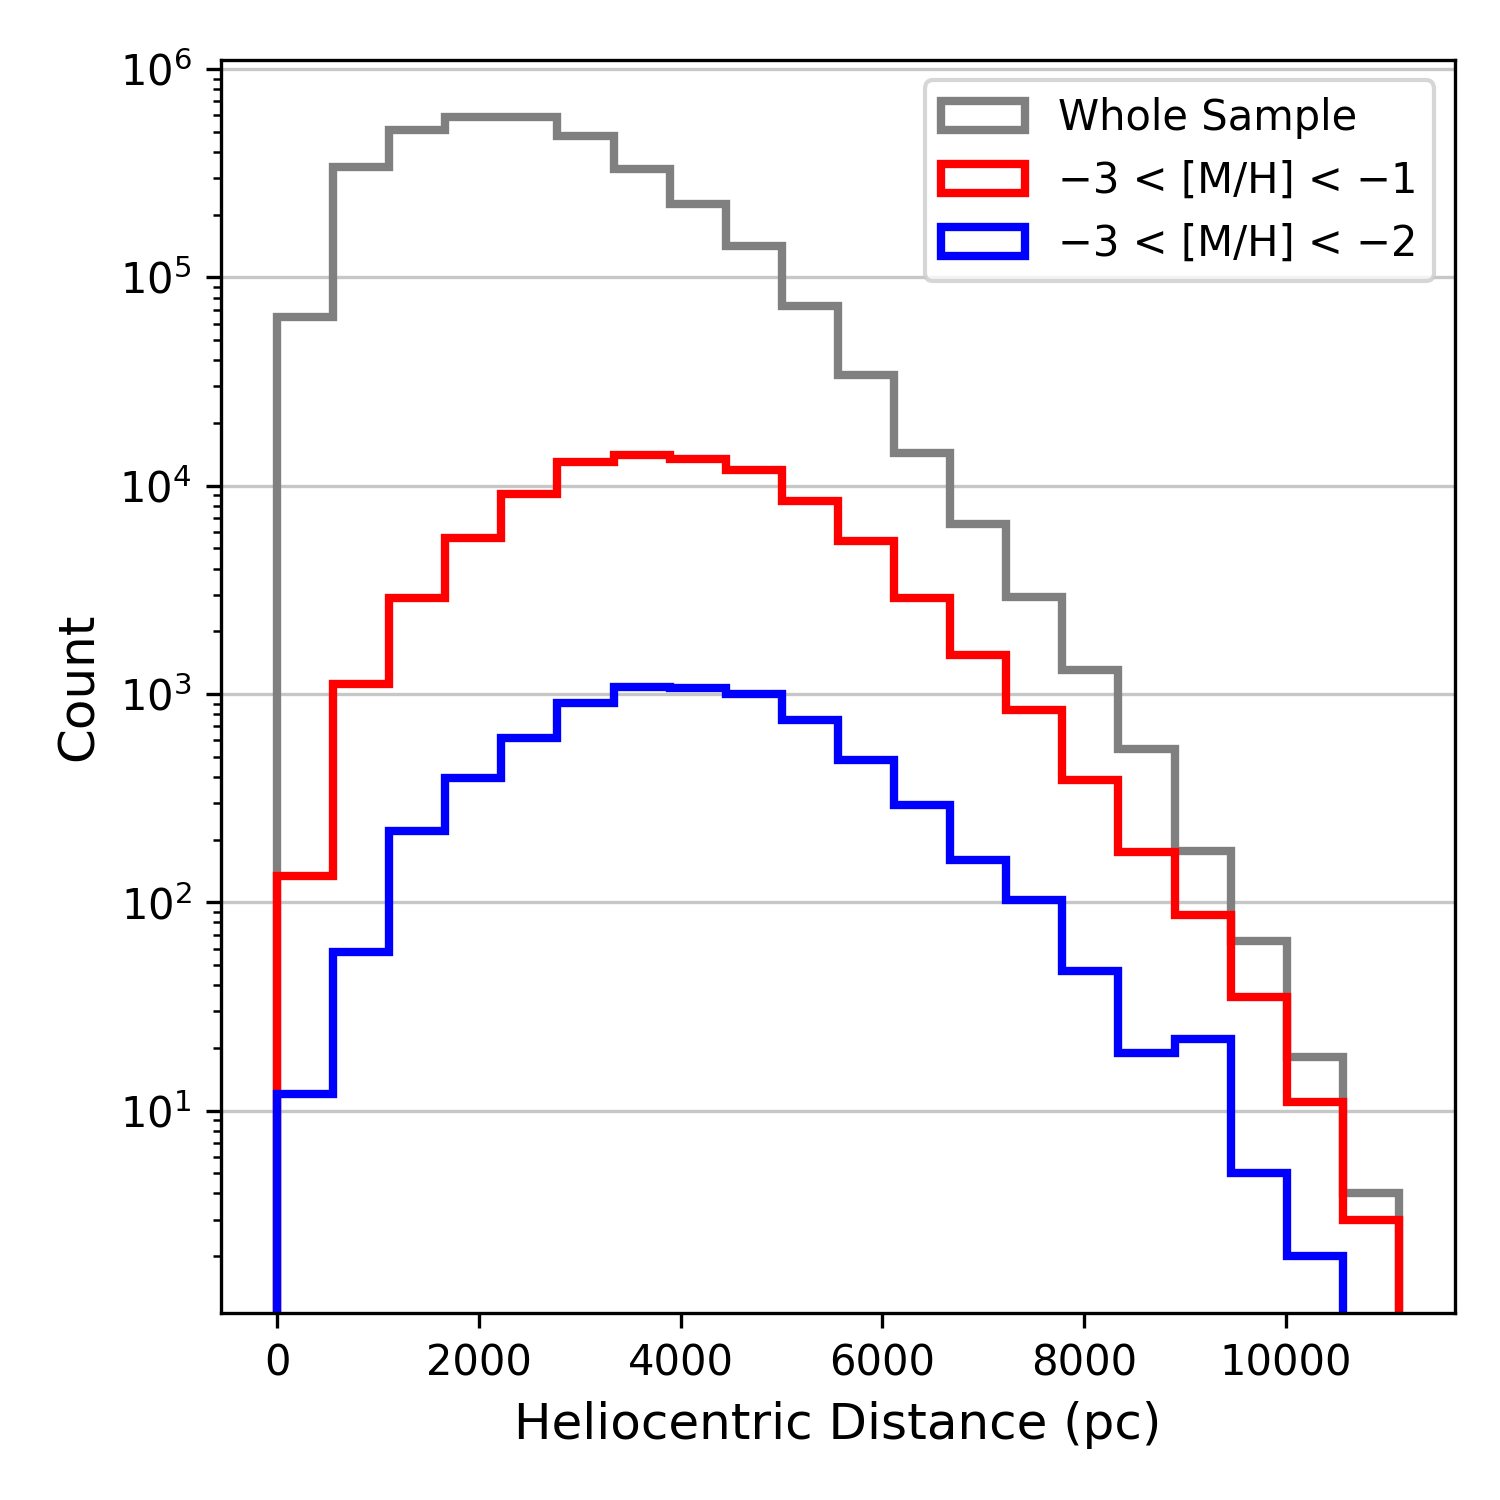
\includegraphics[width=\textwidth]{../figures/distance_histogram.png}
    \caption{Heliocentric distance}
    \label{fig:dist_hist}
  \end{subfigure}\hfill
  %--- Middle panel -----------------------------------------------------------
  \begin{subfigure}[b]{0.32\textwidth}
    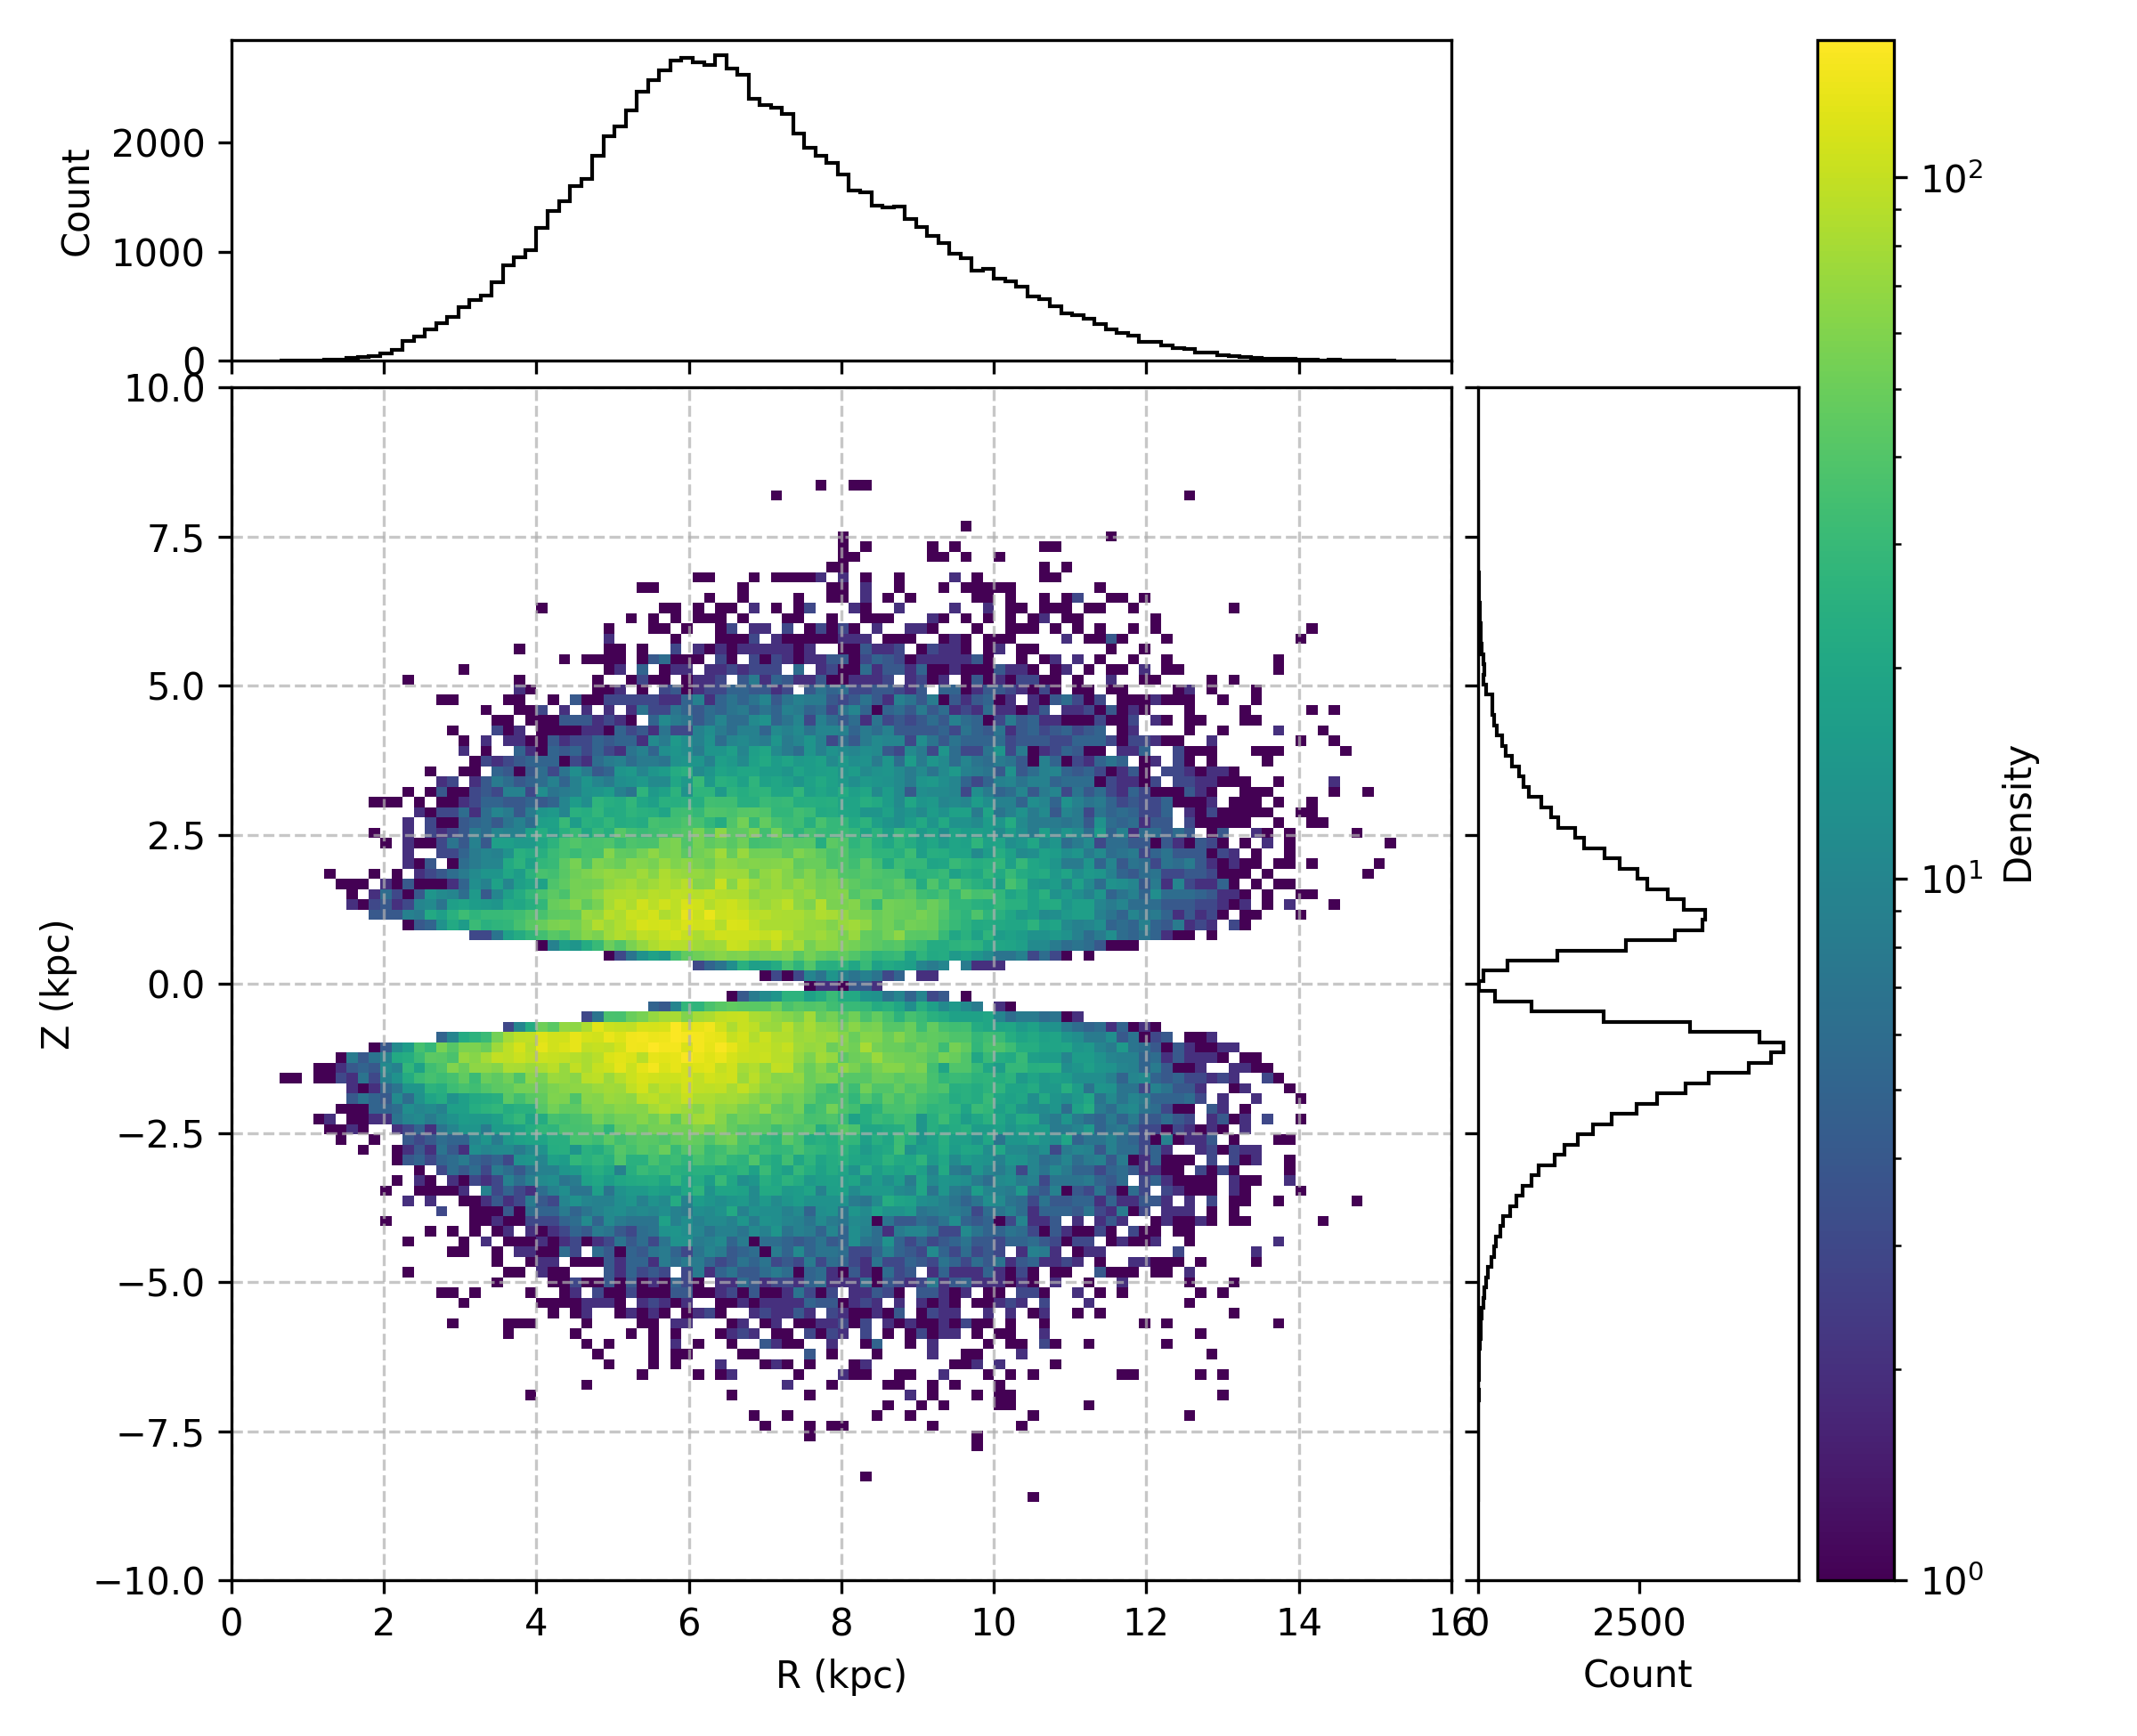
\includegraphics[width=\textwidth]{../figures/ZR_distribution.png}
    \caption{$R$–$Z$ distribution}
    \label{fig:ZR_dist}
  \end{subfigure}\hfill
  %--- Right panel ------------------------------------------------------------
  \begin{subfigure}[b]{0.32\textwidth}
    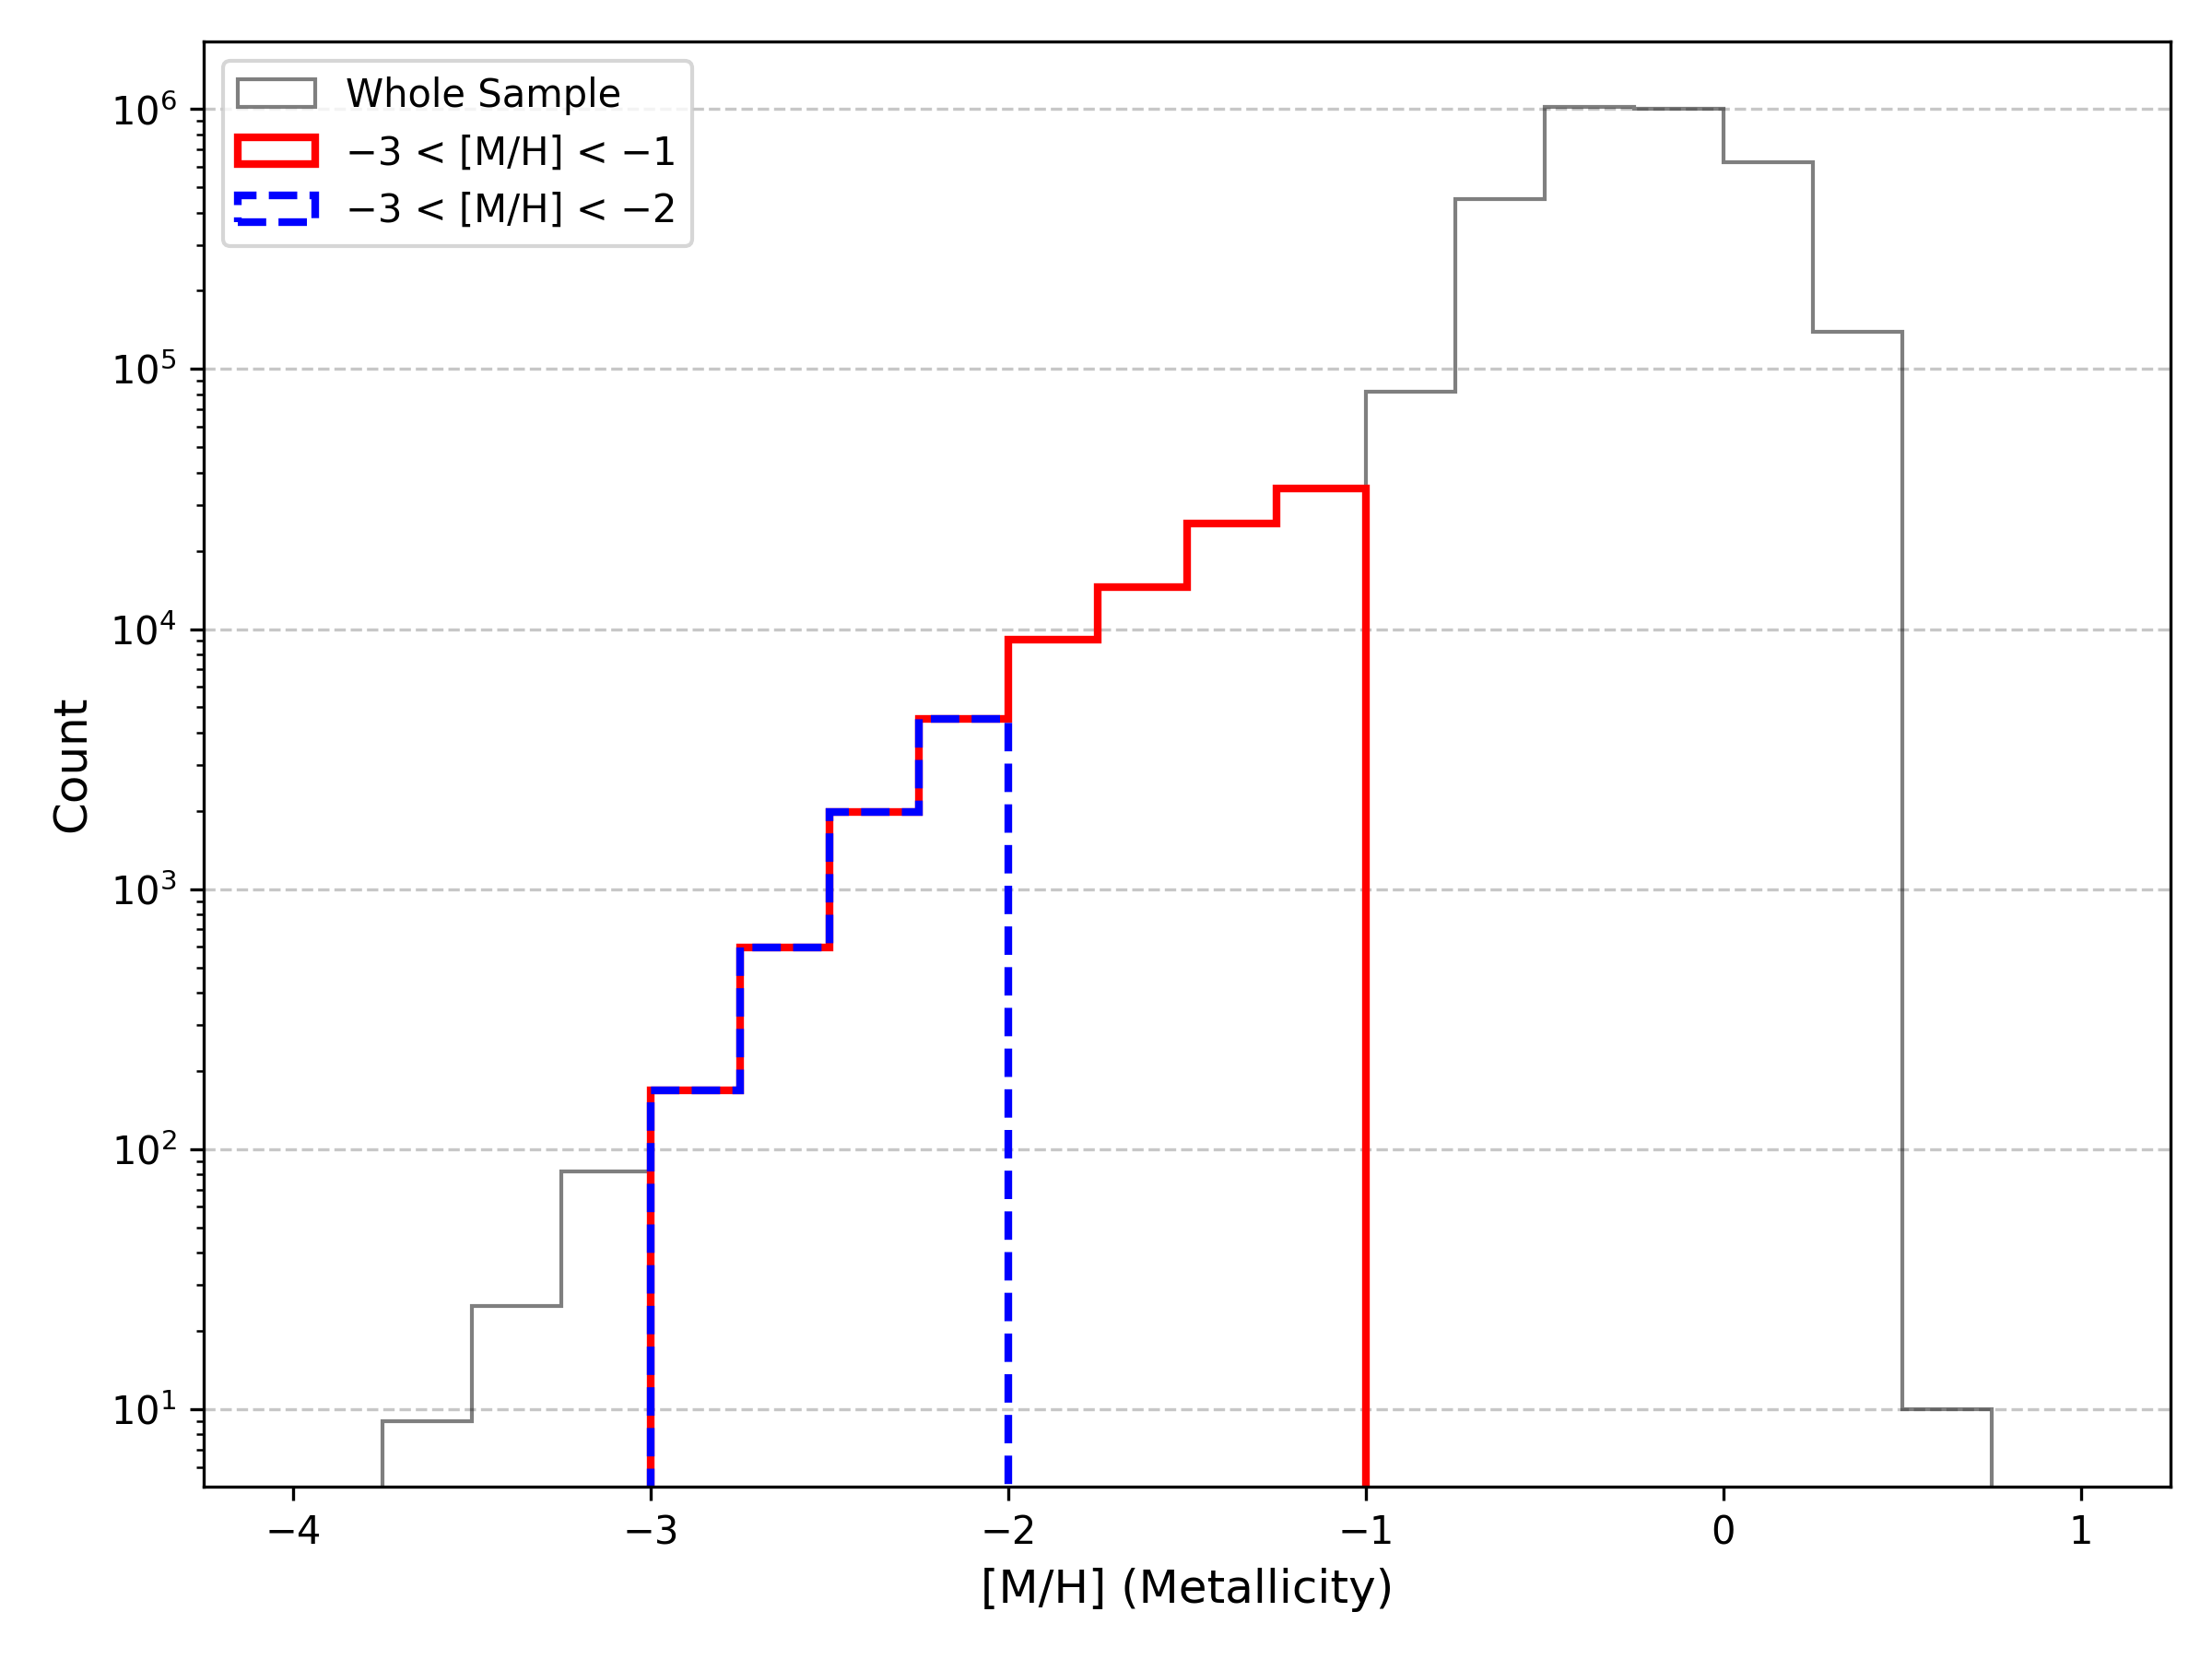
\includegraphics[width=\textwidth]{../figures/metallicity_distribution.png}
    \caption{Metallicity}
    \label{fig:met_dist}
  \end{subfigure}

  \caption{Properties of the final RGB sample after all quality and footprint cuts.
           \textit{Left:} heliocentric-distance histogram for the whole sample (grey); the
           subsets with $-3<\mathrm{[M/H]}<-1$ and $-3<\mathrm{[M/H]}<-2$ are shown in
           solid red and dashed blue, respectively.  
           \textit{Middle:} density map in Galactocentric cylindrical coordinates.  
           The empty band at low $|Z|$ is a selection artefact of our
           latitude/extinction cuts, which deliberately remove the thin–disc mid-plane;
           the concentration around $R\!\simeq\!5$–$8$\,kpc reflects the volume
           accessible to bright RGB stars interior to the Solar circle and coincides
           with the molecular ring region where the stellar surface density peaks.  
           \textit{Right:} Metallicity distribution of our data sample. Line colours are the same as in the left panel.
           (A reproduction of Figure 1 from \citet{zhang2024existencemetalpoordiscmilky})}
  \label{fig:data_properties}
\end{figure}

\subsection{Galactocentric Positions and Velocities}
\label{subsec:velocities}

Six-dimensional phase-space coordinates were obtained with
astropy.coordinates.  We adopted a Galactocentric frame
with $R_{0}=8.1$\,kpc and $Z_{0}=25$\,pc \citep{McMillan2016}, and a solar
velocity. $(U_{\odot},V_{\odot},W_{\odot})=(11.1,\,245,\,7.25)$\,km\,s$^{-1}$
\citep{Schonrich2010}.
The cylindrical velocity components
$(v_{R},v_{\phi},v_{Z})$ were extracted using the transformed
SkyCoord module.

To propagate measurement errors we generated
$N_{\rm MC}=100$ Monte-Carlo realisations per star, drawing
parallax, proper motions, radial velocity, and distance from their
reported uncertainties.  Each realisation was transformed to the
Galactocentric frame, yielding distributions of
$v_{R}$, $v_{\phi}$, and $v_{Z}$; the $1\sigma$ widths of those
distributions were stored as per-star velocity uncertainties.


\begin{figure}
  \centering
  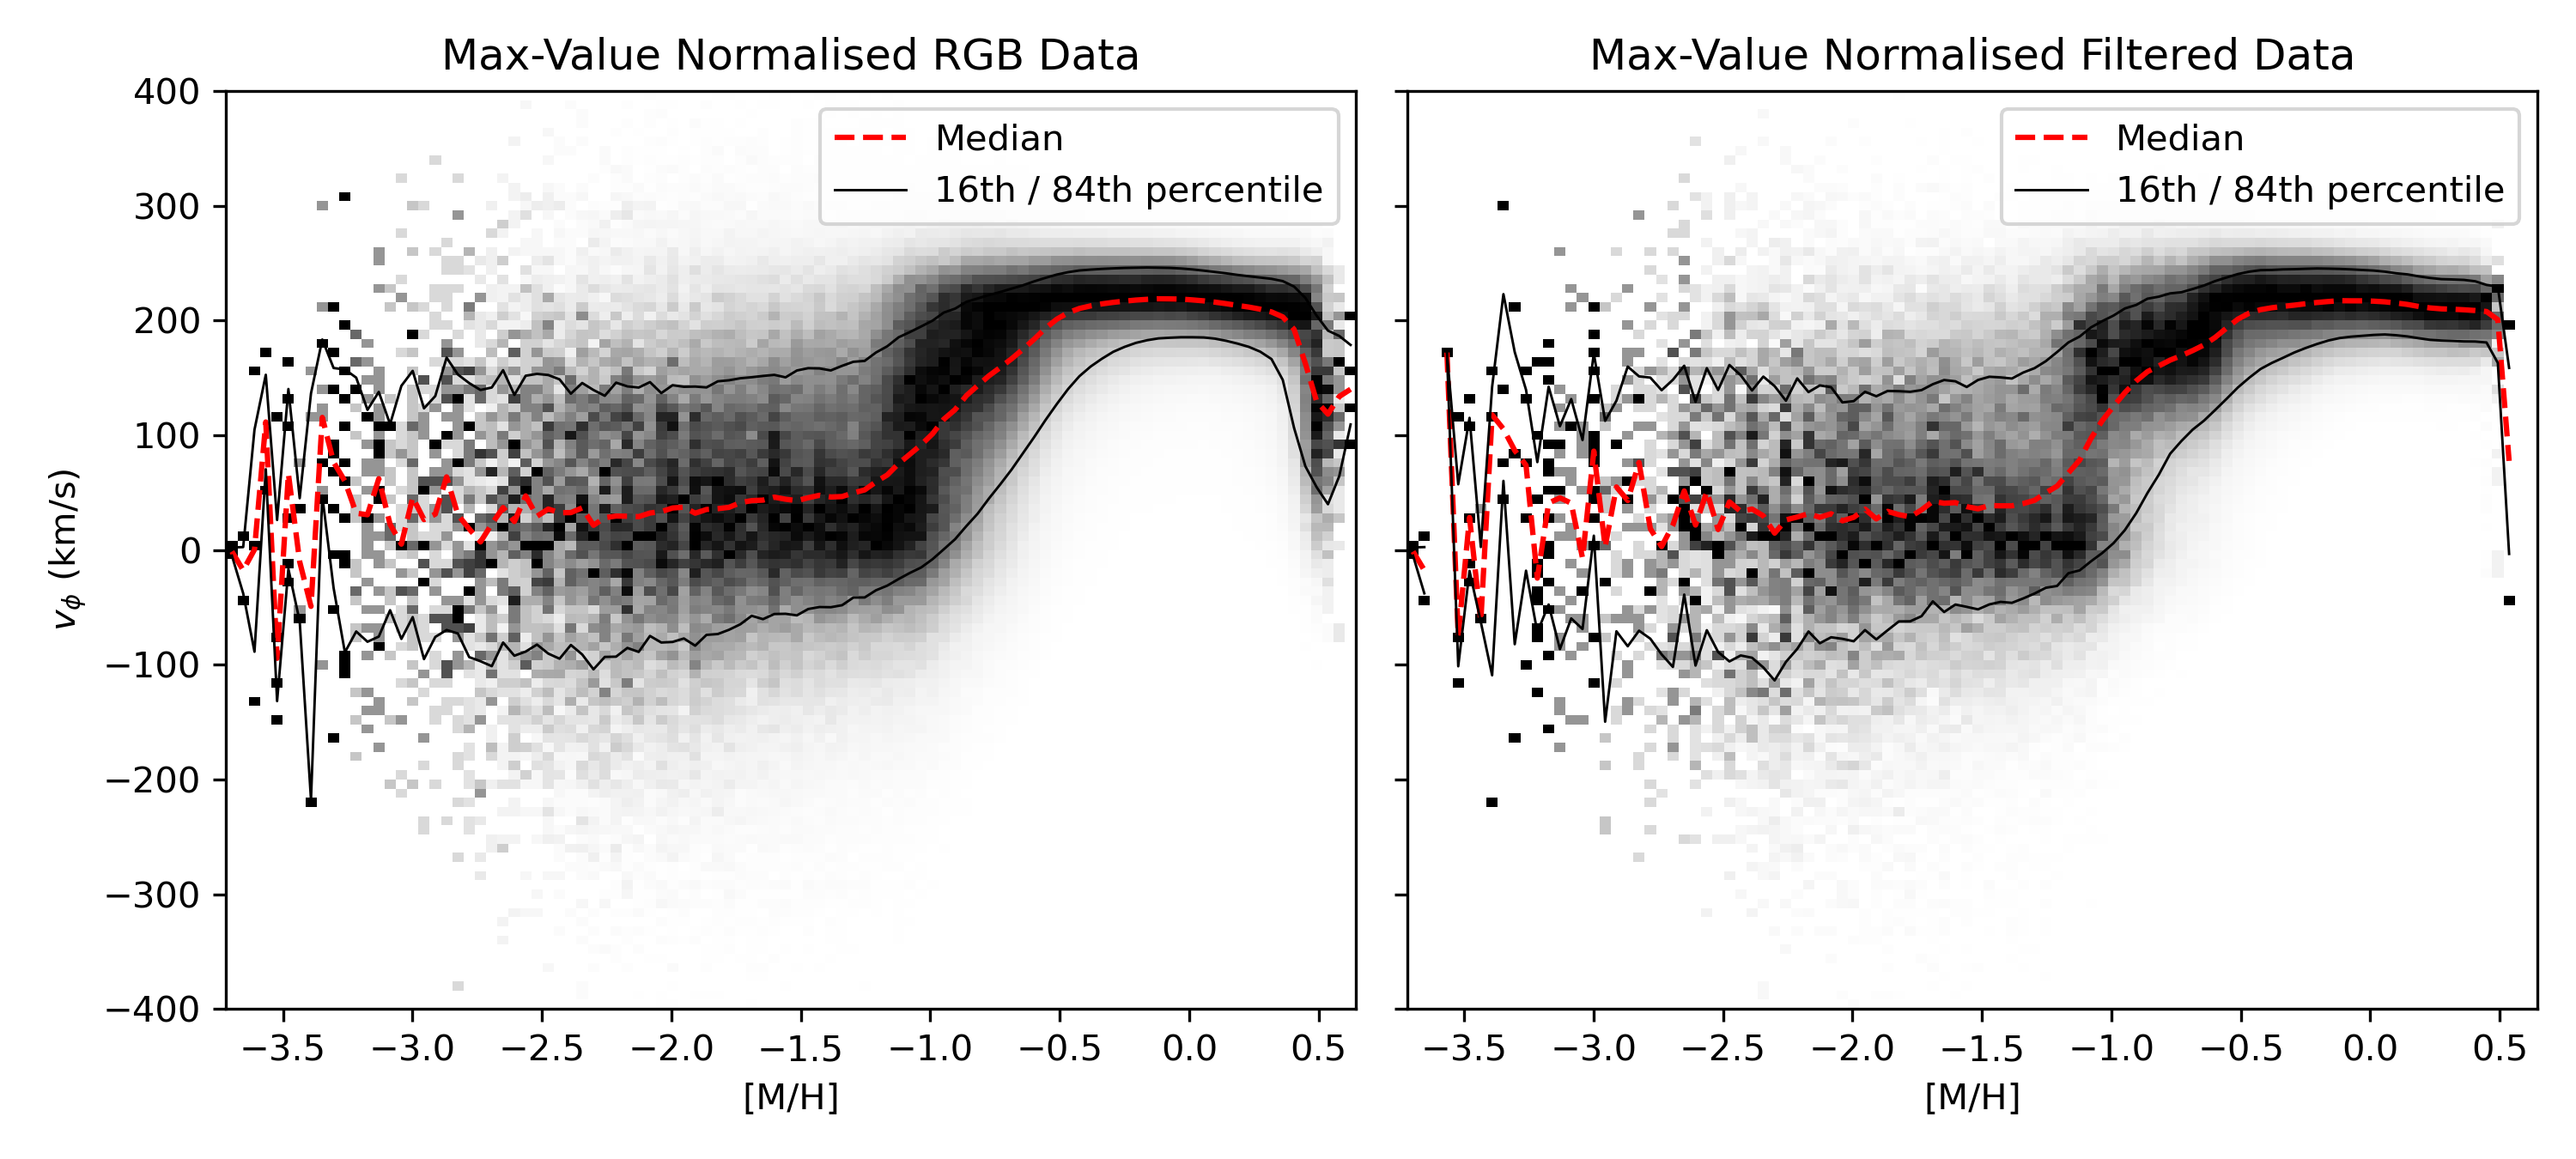
\includegraphics[width=0.94\textwidth]{../figures/vphi_histograms_with_tracks.png}
  \caption{Column-normalised density in the $v_{\phi}$–[M/H] plane.
           \textit{Left:} the bright-RGB catalogue of \citet{Andrae2023}.
           \textit{Right:} the same sample after all distance,
           dust, and quality cuts.  Greyscale pixels show the normalised
           counts in each metallicity bin; the red dashed curve is the
           median $v_{\phi}$, and the black curves trace the 16$^{\text{th}}$
           and 84$^{\text{th}}$ percentiles.
           (A reproduction of Figure 2 from \citet{zhang2024existencemetalpoordiscmilky})}
  \label{fig:vphi_tracks}
\end{figure}



Stellar azimuthal velocities
evolve increase with metallicity as shown in Figure~\ref{fig:vphi_tracks}.  
Halo-like kinematics dominate at
${\rm [M/H]}\lesssim-1.5$ with statistics
indicative of a pressure-supported component.  A spin-up appears over the 
metallicity range ${\rm [M/H]} \simeq -1.3$ to $-0.9$, consistent with \citet{Belokurov2022} and with Figure~\ref{fig:vphi_tracks}.
By ${\rm [M/H]}\gtrsim-0.5$ the stellar azimuthal velocities reaches the Local
Standard-of-Rest value ($\approx220\;\mathrm{km\;s^{-1}}$) and the
velocity dispersion dispersion falls, marking the
transition to a disc.  



\begin{figure}
  \centering
  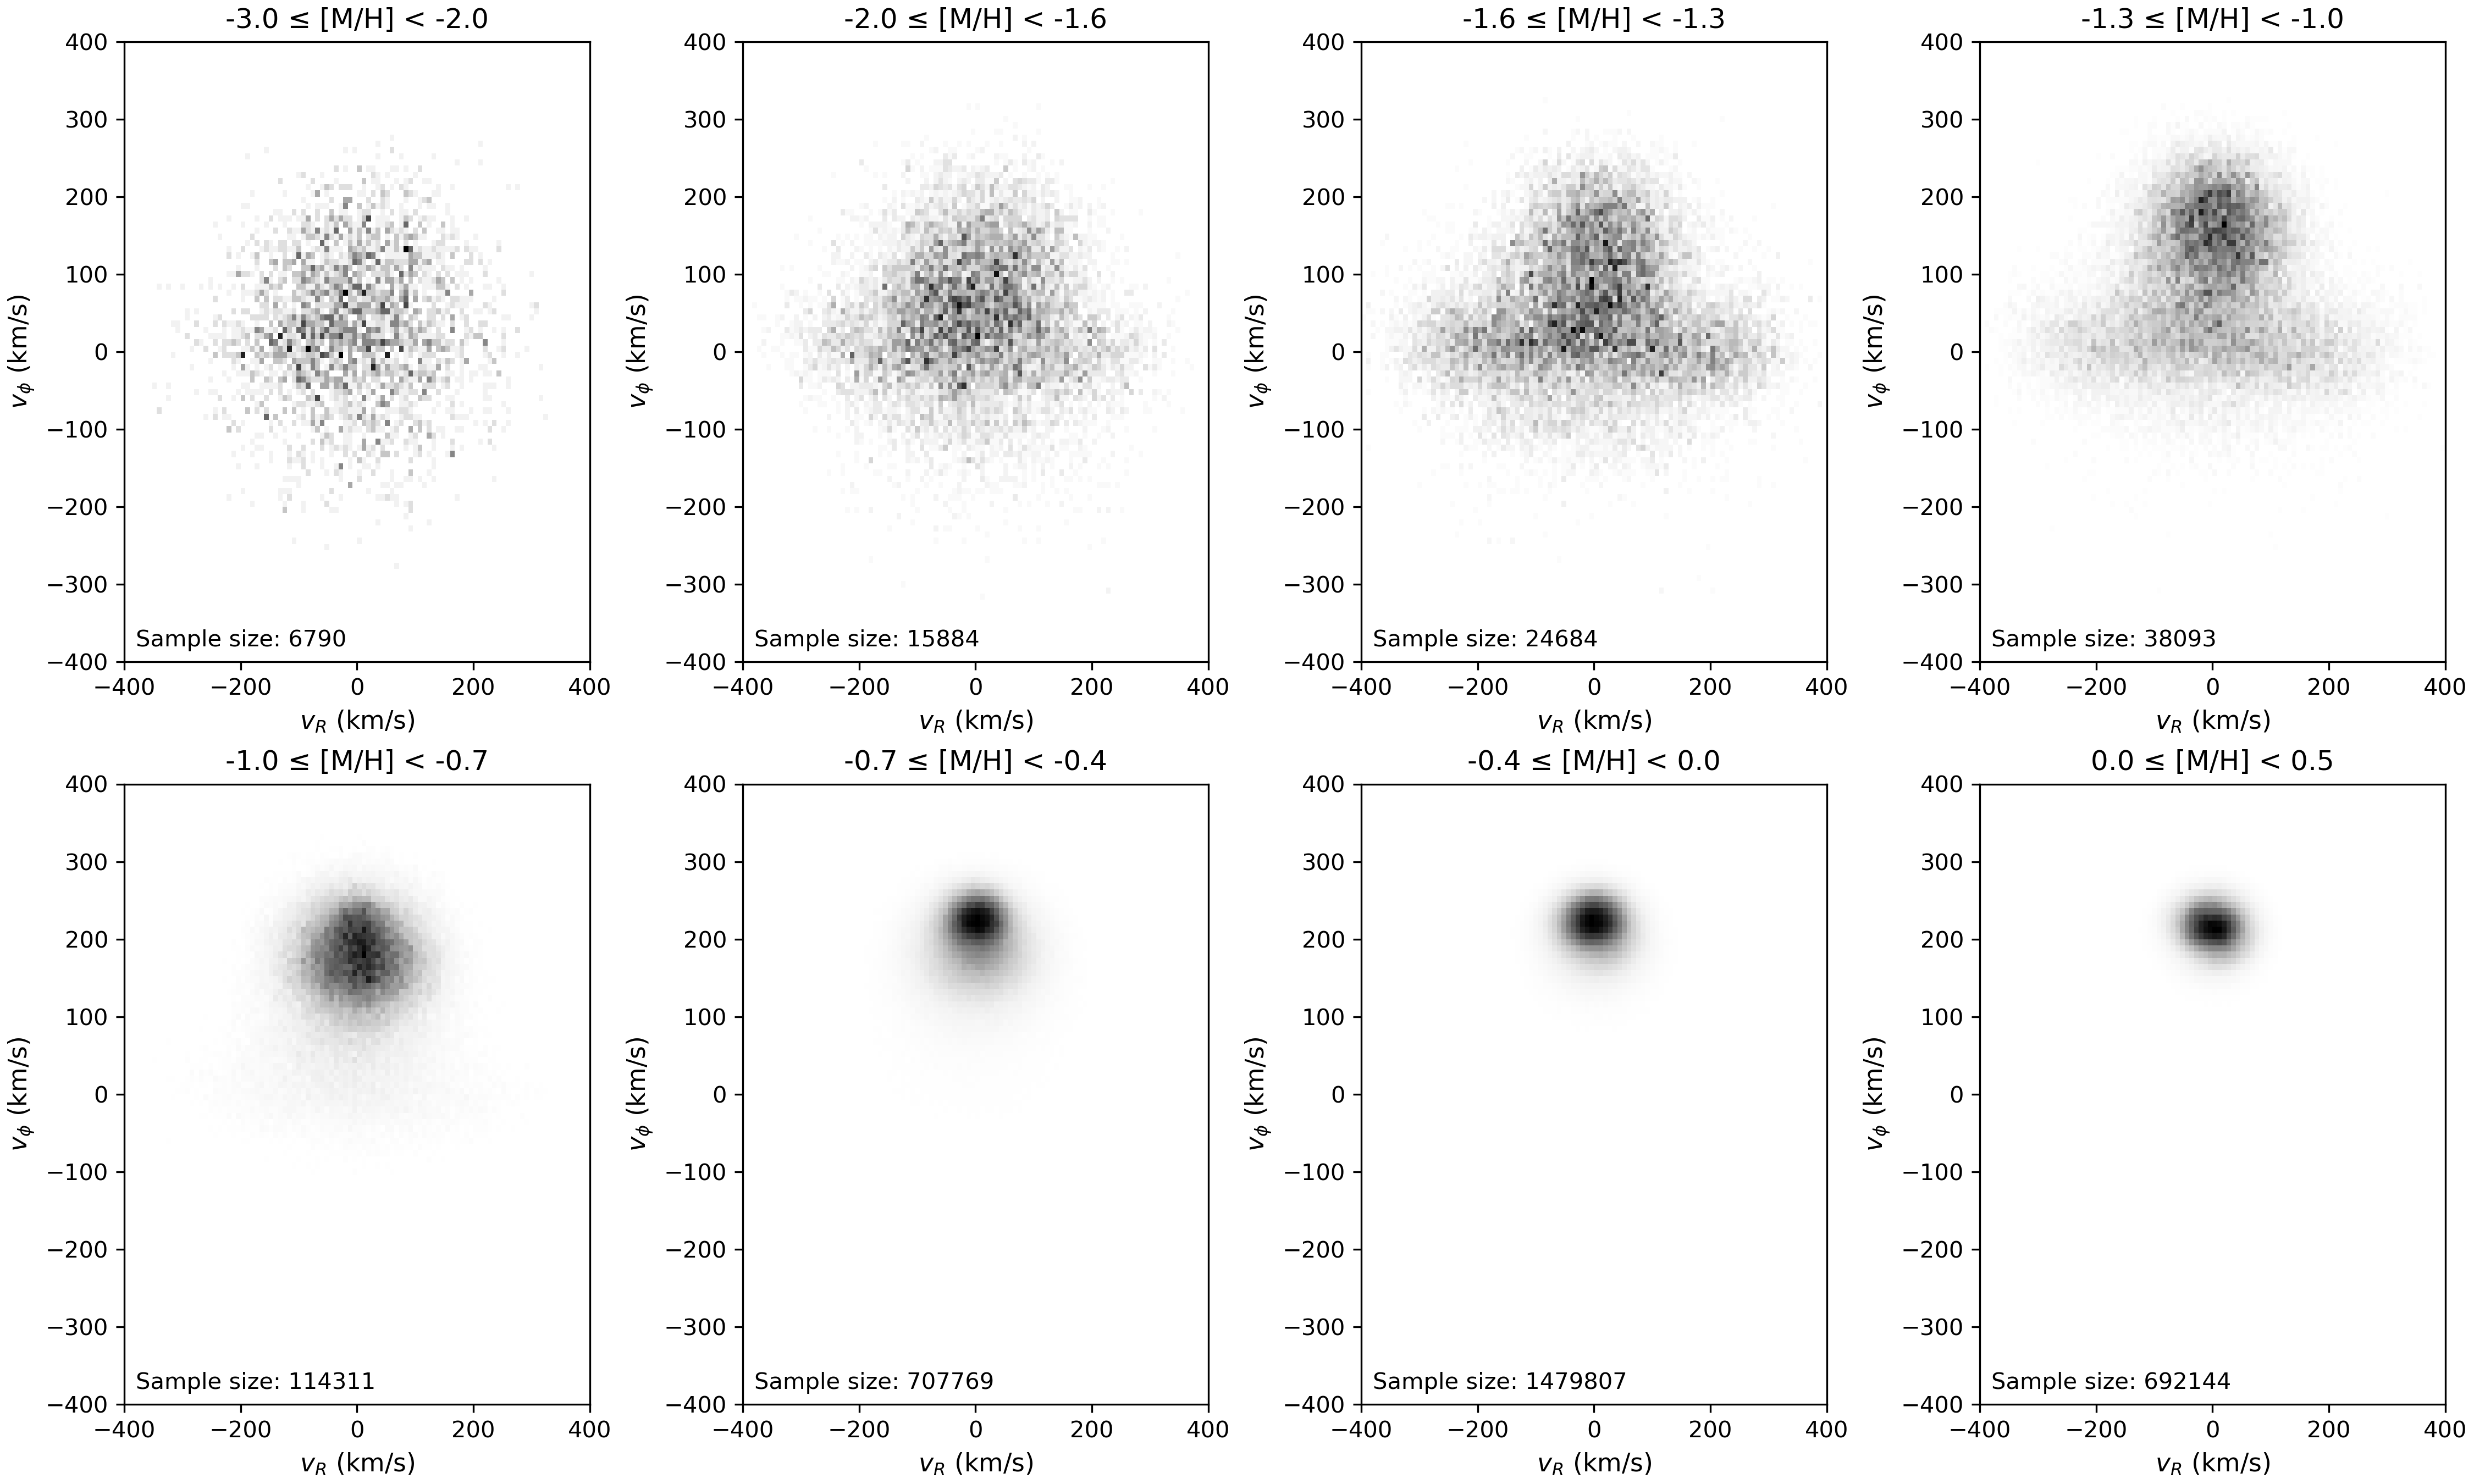
\includegraphics[width=\textwidth]
                   {../figures/vphi_metallicity_histograms.png}
  \caption{Galactocentric velocity distributions as a function of metallicity.
           Each panel shows the column–normalised density of stars in the
           $v_R$–$v_\phi$ plane for the metallicity interval printed at the
           top.(A reproduction of Figure 3 from \citet{zhang2024existencemetalpoordiscmilky})
           }
  \label{fig:vRvphi_bins}
\end{figure}

\begin{figure}
  \centering
  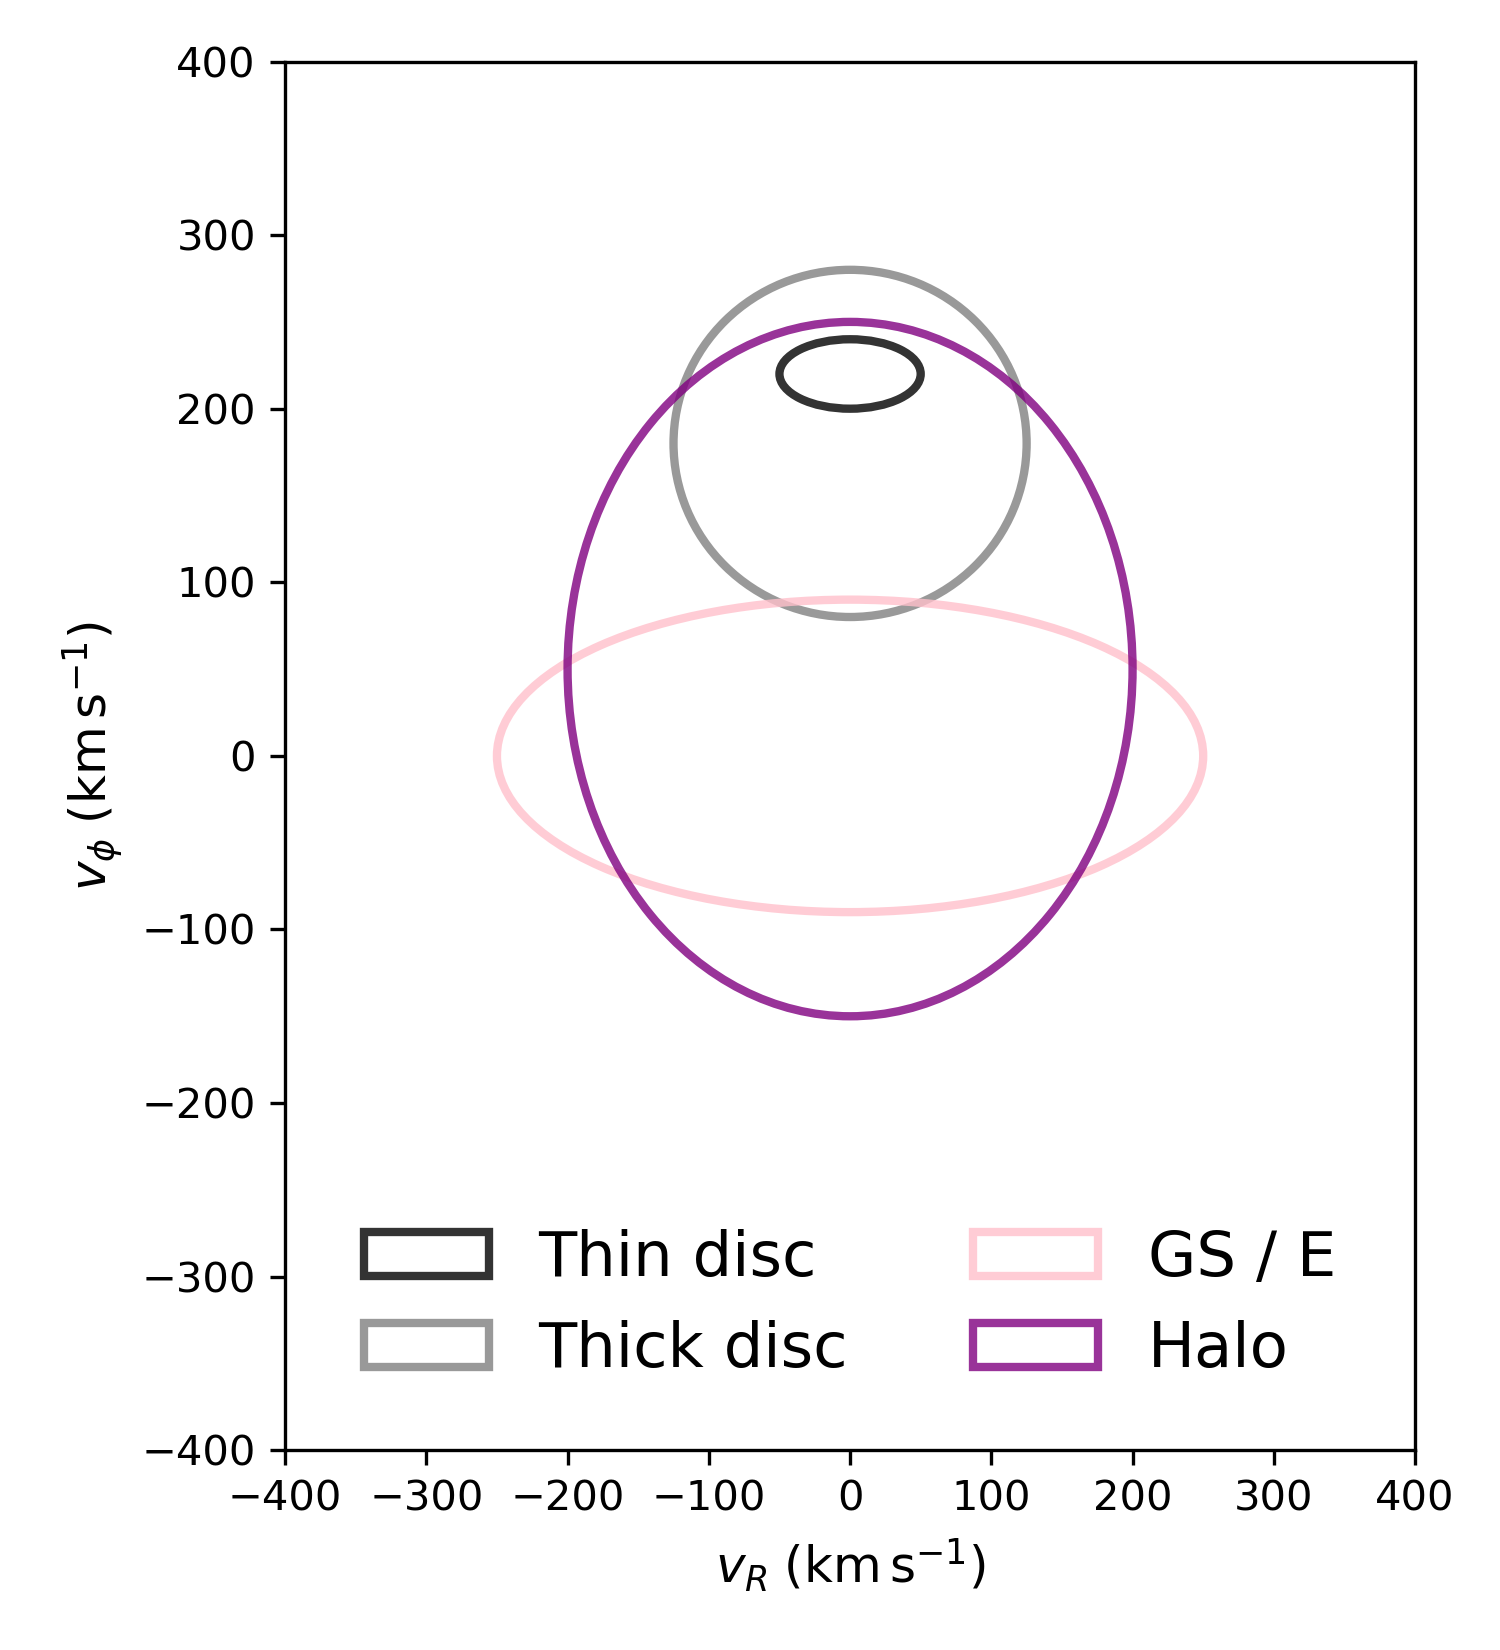
\includegraphics[width=0.3\columnwidth]
                   {../figures/reference_velocity_ellipses.png}
  \caption{Ellipses mark the approximate extent of the thin disc
           (black), thick disc (gray),
           Gaia–Sausage/Enceladus debris (pink) and the
           pressure-supported stellar halo (purple).
           The figure should be used as a visual key for interpreting the data panels
           in Fig.~\ref{fig:vRvphi_bins}.
           }
  \label{fig:ref_ellipses}
\end{figure}

As shown in Fig.~\ref{fig:vRvphi_bins}, stars with
${\rm[M/H]}\!\geq\!-1.0$ have a strong prograde bias in azimuthal velocities, 
with a peak at $v_\phi\!\gtrsim\!180$ km s$^{-1}$ and a relatively narrow
distribution in $v_R$. This is consistent with 
the thin- and thick-disc ellipses (Fig.~\ref{fig:ref_ellipses}). 
Below ${\rm[M/H]}\simeq-1.0$ the distribution broadens and
drops toward $v_\phi\!\approx\!0$, indicating
pressure supported kinematics, characteristic of the stellar halo and
the radial Gaia-Sausage/Enceladus debris.  At the lowest
metallicities (${\rm[M/H]}\lesssim-1.5$) the contours are nearly
isotropic with only a mild prograde bias.  Hence, any
rotation-supported very-metal-poor disc must contribute at most a
small fraction of the population. In subsequent analysis we quantitatively assess
these observations.


\section{Methodology}

\subsection{Gaussian Mixture Model}

As in \citet{zhang2024existencemetalpoordiscmilky}, to quantitatively investigate the kinematic structure of metal-poor stars and assess 
the presence of a potential very-metal-poor disc, we use a Gaussian Mixture Model (GMM) framework. 
GMMs are a class of unsupervised machine learning algorithms commonly used in data science 
for clustering and density estimation. They model a dataset as a weighted sum of multivariate 
Gaussian distributions, each corresponding to a latent sub-population within the data.

From a probabilistic perspective, the GMM assumes that each observed data point is generated from a 
hidden (latent) variable indicating membership in one of the Gaussian components. This latent space 
formulation allows the model to assign probabilistic classifications to data points, providing a 
soft clustering where each star has a fractional likelihood of belonging to each component. In our case, 
the data is the three-dimensional velocity vectors $(v_R, v_\phi, v_Z)$, and the latent space captures 
distinct kinematic substructures in this space.

The mixture fitting is carried out with \texttt{pyGMMis} \citep{pygmmis} in the full $(v_R,v_\phi,v_Z)$ 
phase space. The code implements the \emph{extreme-deconvolution} extension of the Expectation-Maximisation 
algorithm \citep{Bovy2011}: at every EM iteration each trial Gaussian is \emph{convolved} with the star-specific 
$3{\times}3$ velocity-error matrix supplied by Gaia. In doing so, the procedure fit directly for the 
\textit{intrinsic} (noise-free) velocity distribution, accounting for measurement uncertainties and 
preventing them from creating or erasing kinematic structure—thereby placing all subsequent disc/halo 
classifications on a statistically robust footing.


\subsection{Number of Gaussian Components}
\label{subsec:n_components}

We run the XD–GMM in successive 0.3-dex slices across the regime
\([\mathrm{M/H}]<-1\), the only metallicity range where an undiscovered
very-metal-poor disc could plausibly reside.  Treating each slice
independently removes the steep disc gradient in \([\mathrm{M/H}]\) and allows the
algorithm to search for rotation-supported structure at a fixed chemical
epoch.  Within every slice the optimal number of Gaussians, \(k\), is chosen
by the Bayesian Information Criterion (BIC \citealt{Schwarz1978}: selecting too few components
would blur distinct populations together and mask a genuine disc,
whereas too many would shatter the halo into noise-driven shards and
produce an over-fit, physically meaningless solution.

The BIC is defined as

\begin{equation}
\mathrm{BIC} = k \ln(n) - 2 \ln \mathcal{L},
\end{equation}

where $k = (1 + 3 + 6) \times N - 1$ is the total number of free parameters in a model with $N$ Gaussian components 
(accounting for the weights, means, and covariances), $n$ is the number of stars in the sample, and $\mathcal{L}$ 
is the maximum likelihood of the fit. The BIC penalizes model complexity, such that adding extra components 
without a significant gain in likelihood will result in a higher BIC value.

The Expectation-Maximisation algorithm can become trapped in local minima
because the likelihood surface of a Gaussian mixture is highly
non-convex: overlapping components, label permutations and sparsely sampled
regions generate many secondary peaks, and EM (being a purely uphill
optimiser) has no built-in mechanism for escaping the first peak it reaches.
To minimise this risk we ran 50 independent initialisations for every
candidate component number~\(N\), each time seeding the means with
\(k\)-means initialisation on the \((v_R,v_\phi,v_z)\) data.  The \(k\)-means start-up
partitions the velocity space into compact, nearly spherical groups that match
the Gaussian assumption, giving EM a stable launch point and accelerating
convergence.  For every run we logged the BIC
and adopted the mixture with the lowest BIC overall.  This multi-start,
\(k\)-means-seeded strategy reduces the chance of local-minimum
entrapment and makes it highly likely that the selected model represents the
global maximum-likelihood, and therefore statistically preferred, description of
the data.


\begin{figure*}[h]
    \centering
    \begin{subfigure}[t]{0.23\textwidth}
        \centering
        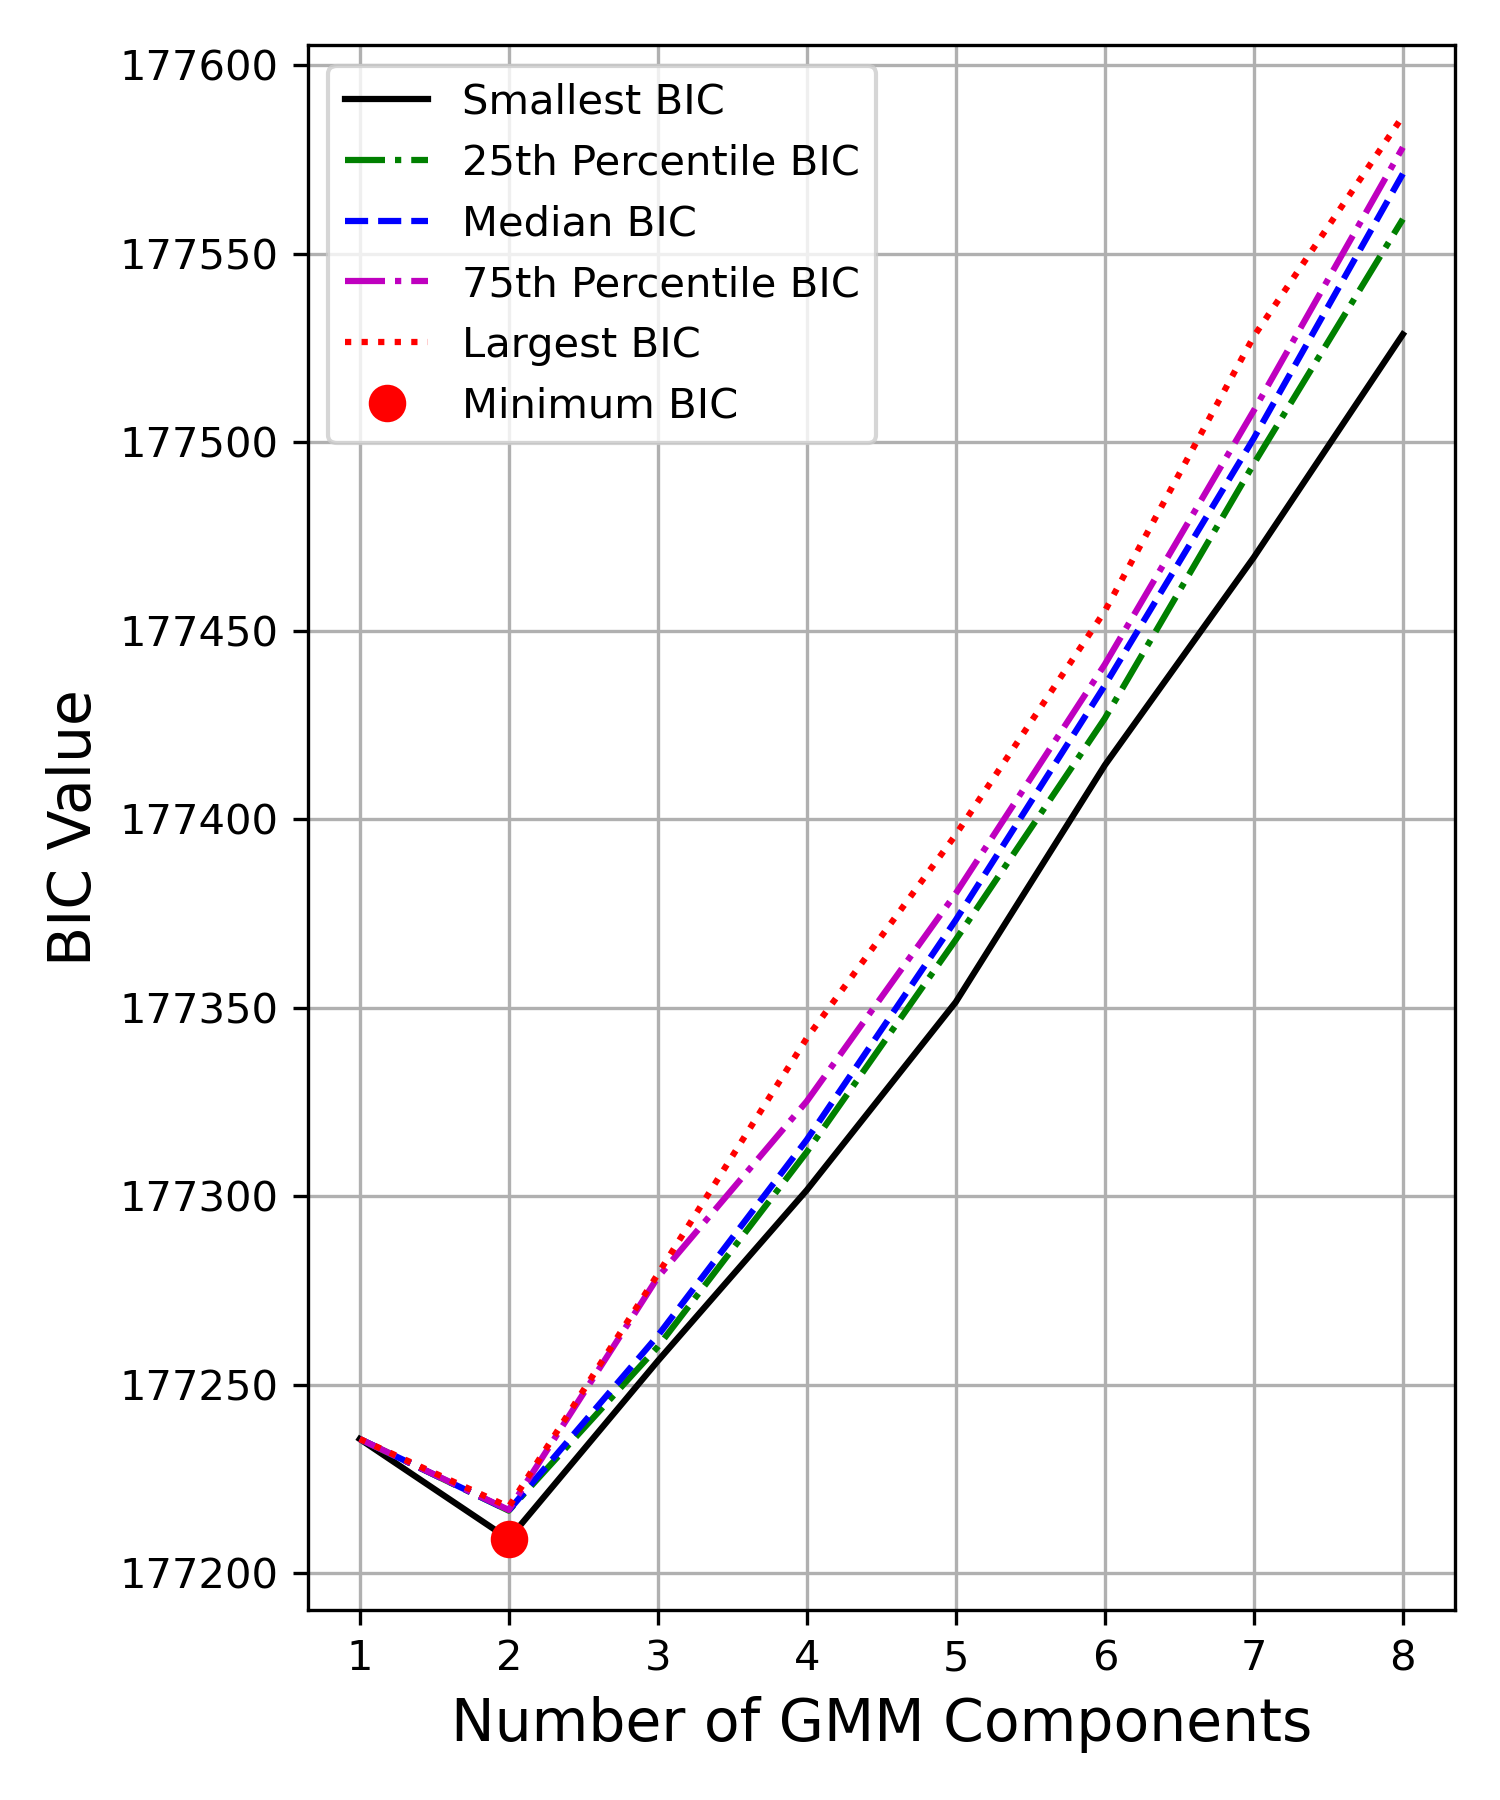
\includegraphics[width=\linewidth]{../figures/bic_vmp.png}
        \caption{$-3.0 < \mathrm{[M/H]} < -2.0$}
    \end{subfigure}
    \hfill
    \begin{subfigure}[t]{0.23\textwidth}
        \centering
        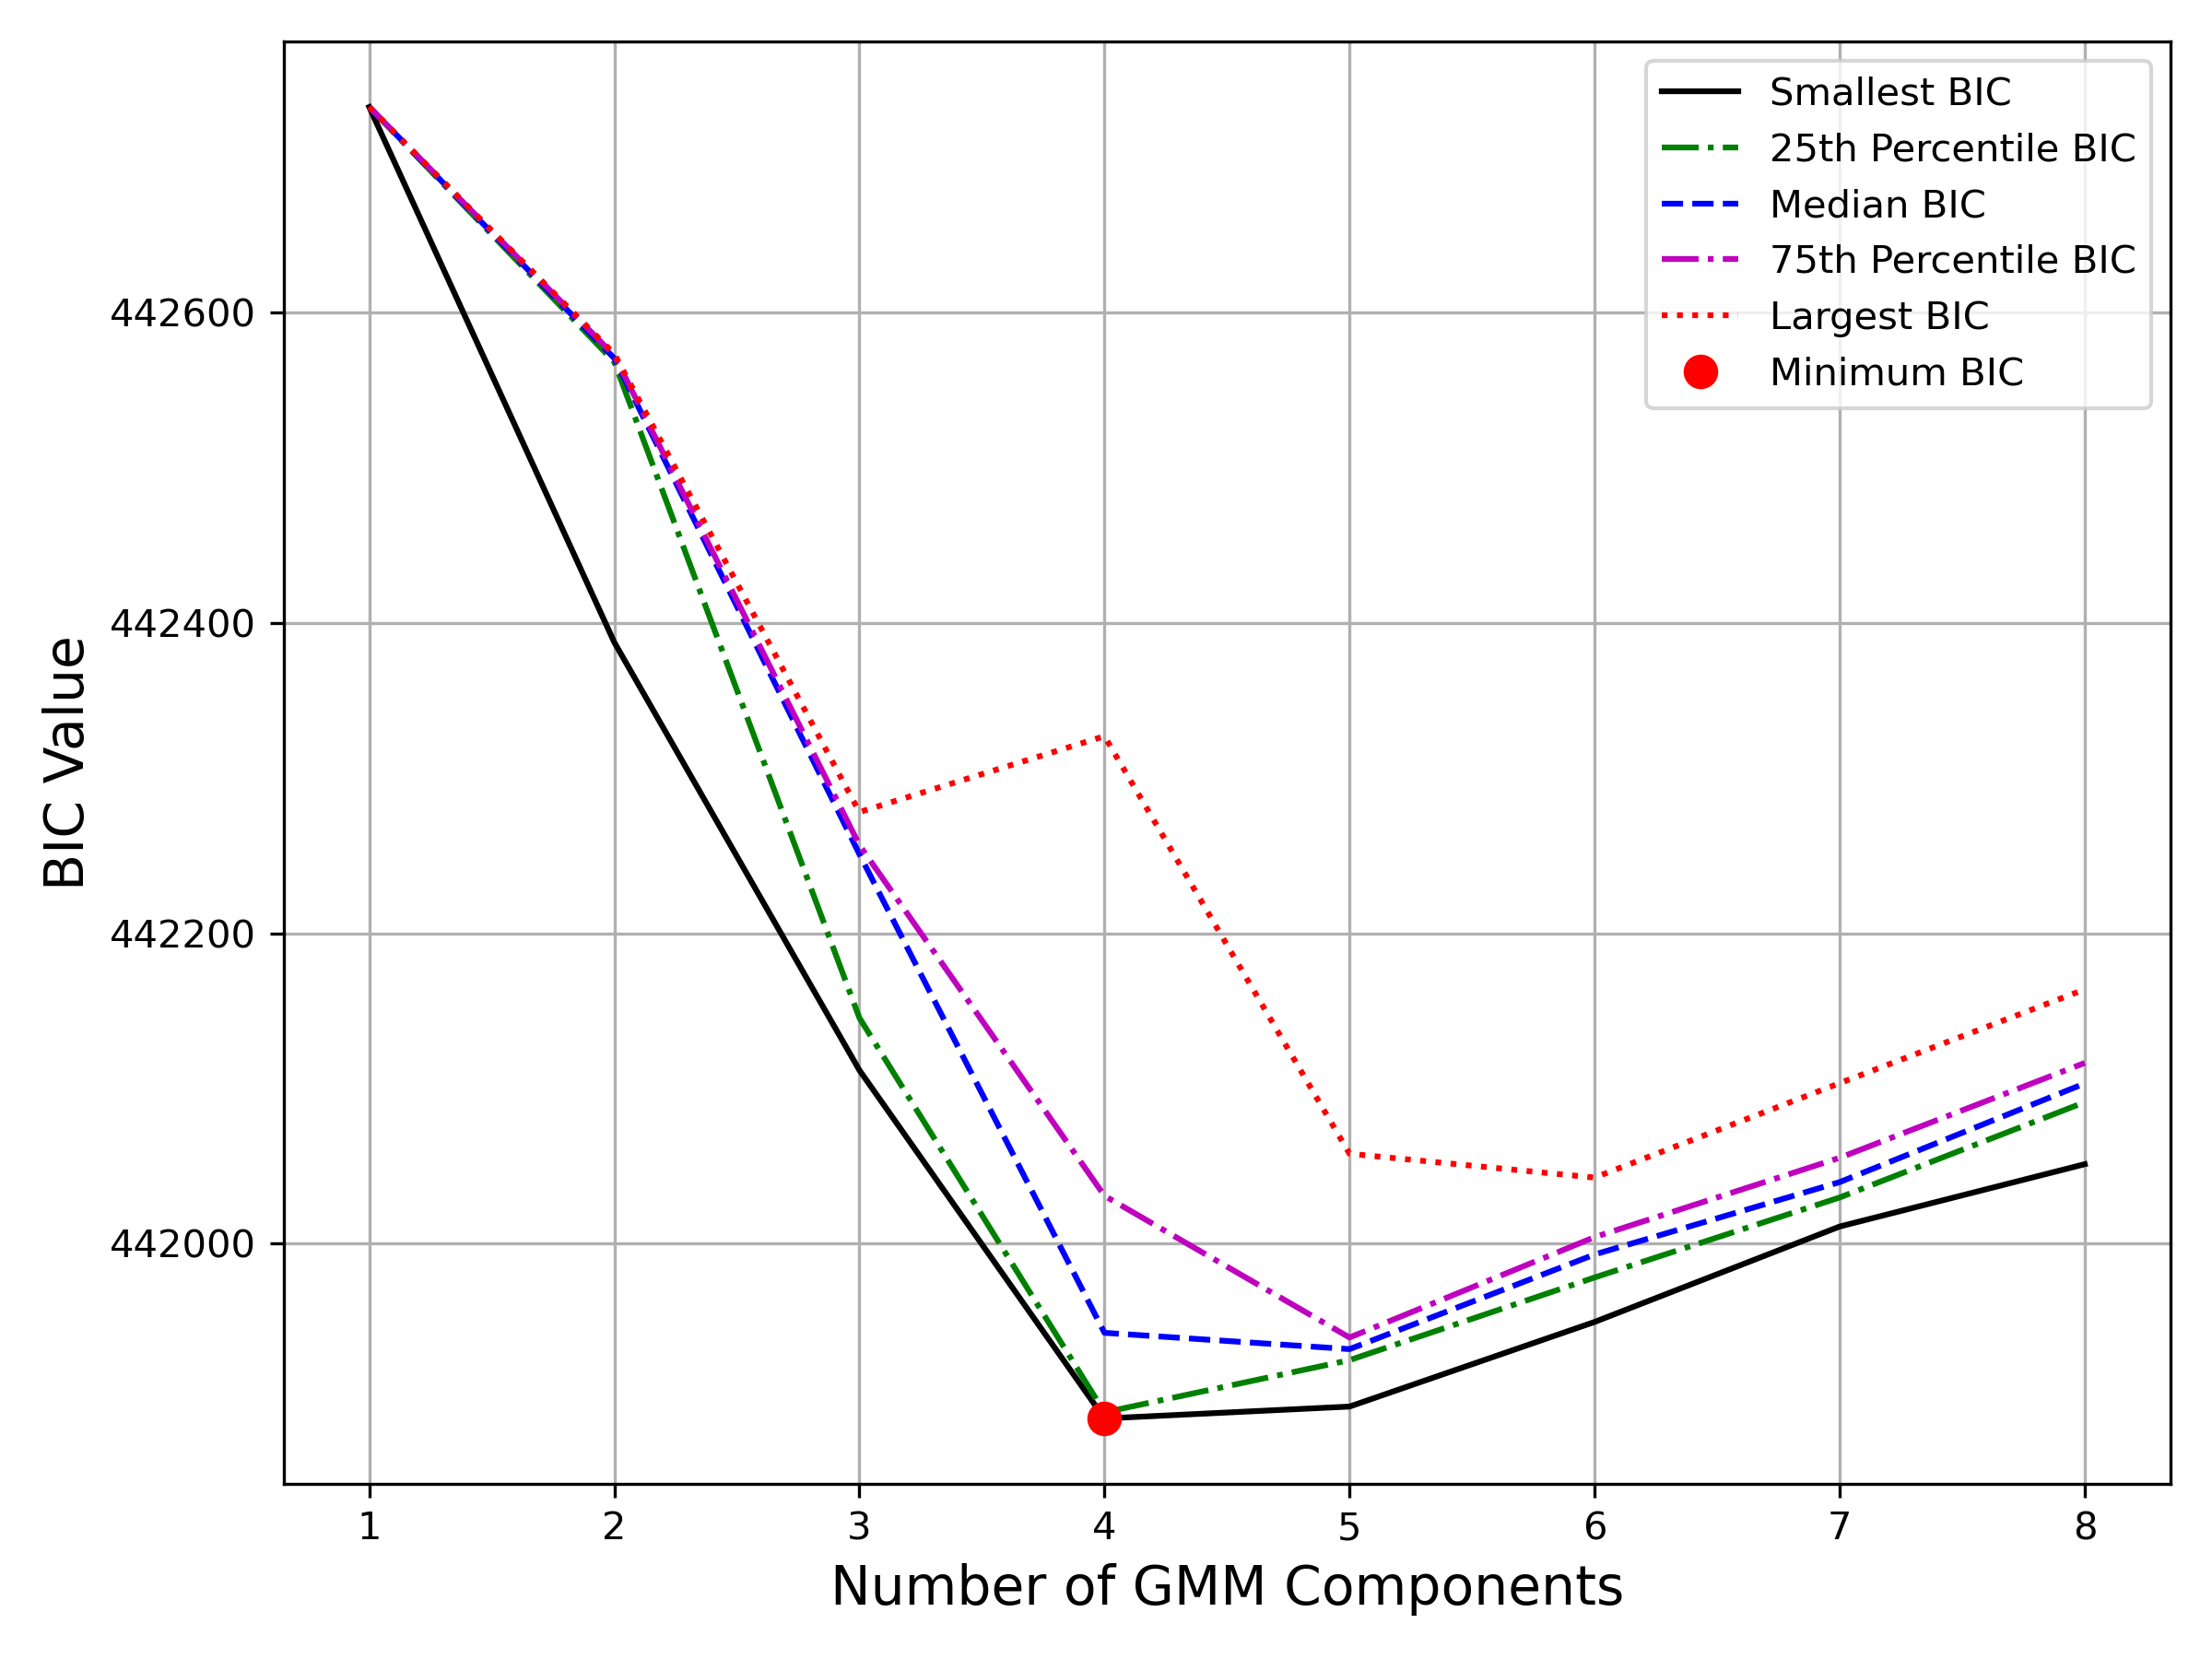
\includegraphics[width=\linewidth]{../figures/bic_imp.png}
        \caption{$-2.0 < \mathrm{[M/H]} < -1.6$}
    \end{subfigure}
    \hfill
    \begin{subfigure}[t]{0.23\textwidth}
        \centering
        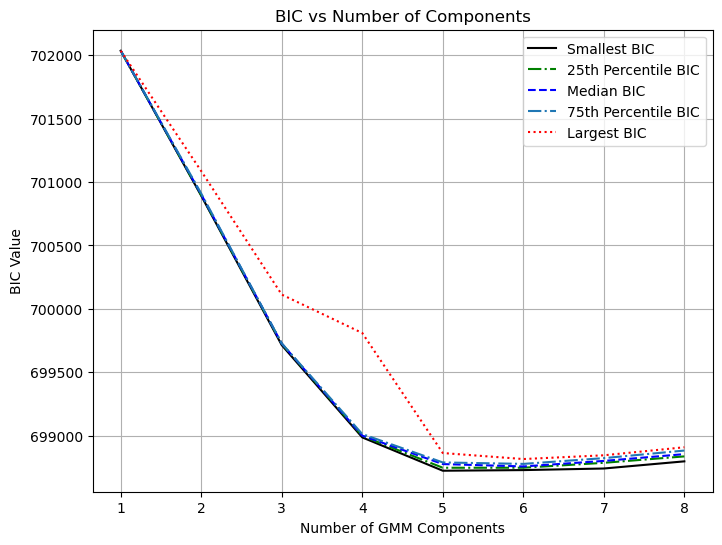
\includegraphics[width=\linewidth]{../figures/bic_mp1.png}
        \caption{$-1.6 < \mathrm{[M/H]} < -1.3$}
    \end{subfigure}
    \hfill
    \begin{subfigure}[t]{0.23\textwidth}
        \centering
        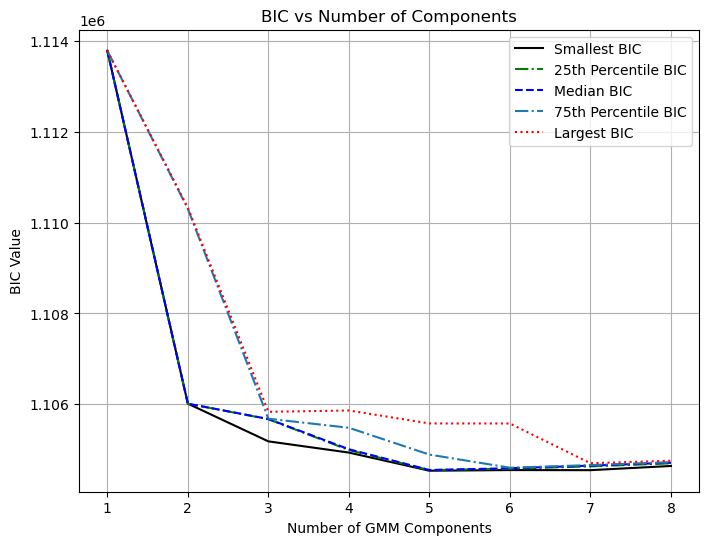
\includegraphics[width=\linewidth]{../figures/bic_mp2.png}
        \caption{$-1.3 < \mathrm{[M/H]} < -1.0$}
    \end{subfigure}

    \caption{BIC distributions as a function of the number of GMM components in each metallicity bin. 
    The optimum number of components is indicated by the minimum BIC value (highlighted in red).
    (A reproduction of Figure 4 from \citet{zhang2024existencemetalpoordiscmilky})}
    \label{fig:bic_vs_n_components}
\end{figure*}




In Figure~\ref{fig:bic_vs_n_components}, we show the distribution of BIC values across four metallicity bins as
a function of $N$. The resulting preferred number of components are 2, 4, 5, and 5 for the VMP, IMP, MP1, and MP2 bins.
This is in agreement with the findings of \citet{zhang2024existencemetalpoordiscmilky}.
Our analysis selects the lowest BIC for each bin, removing the need for a subjective choice of the number of components
when BIC values are very similar. \citet{zhang2024existencemetalpoordiscmilky}, when observing the BIC values for the MP1 bin 
chooses to use 5 components instead of 6 despite the BIC score for the 6-component model being lower than the 5-component model.

 
\section{Results}
\label{sec:results1}

\subsection{Gaussian Mixture Model Fit}
\label{subsec:gmm}

Using the number of components selected by the BIC criteria, we fit the GMM to the data in each metallicity bin as shown in 
Figure~\ref{fig:gmm_decompositions}. We increased the number of initialisations to 100 for the final fitting to ensure convergence to a
stable solution.

\begin{figure*}[h]
    \centering
    \begin{subfigure}[t]{0.24\textwidth}
        \centering
        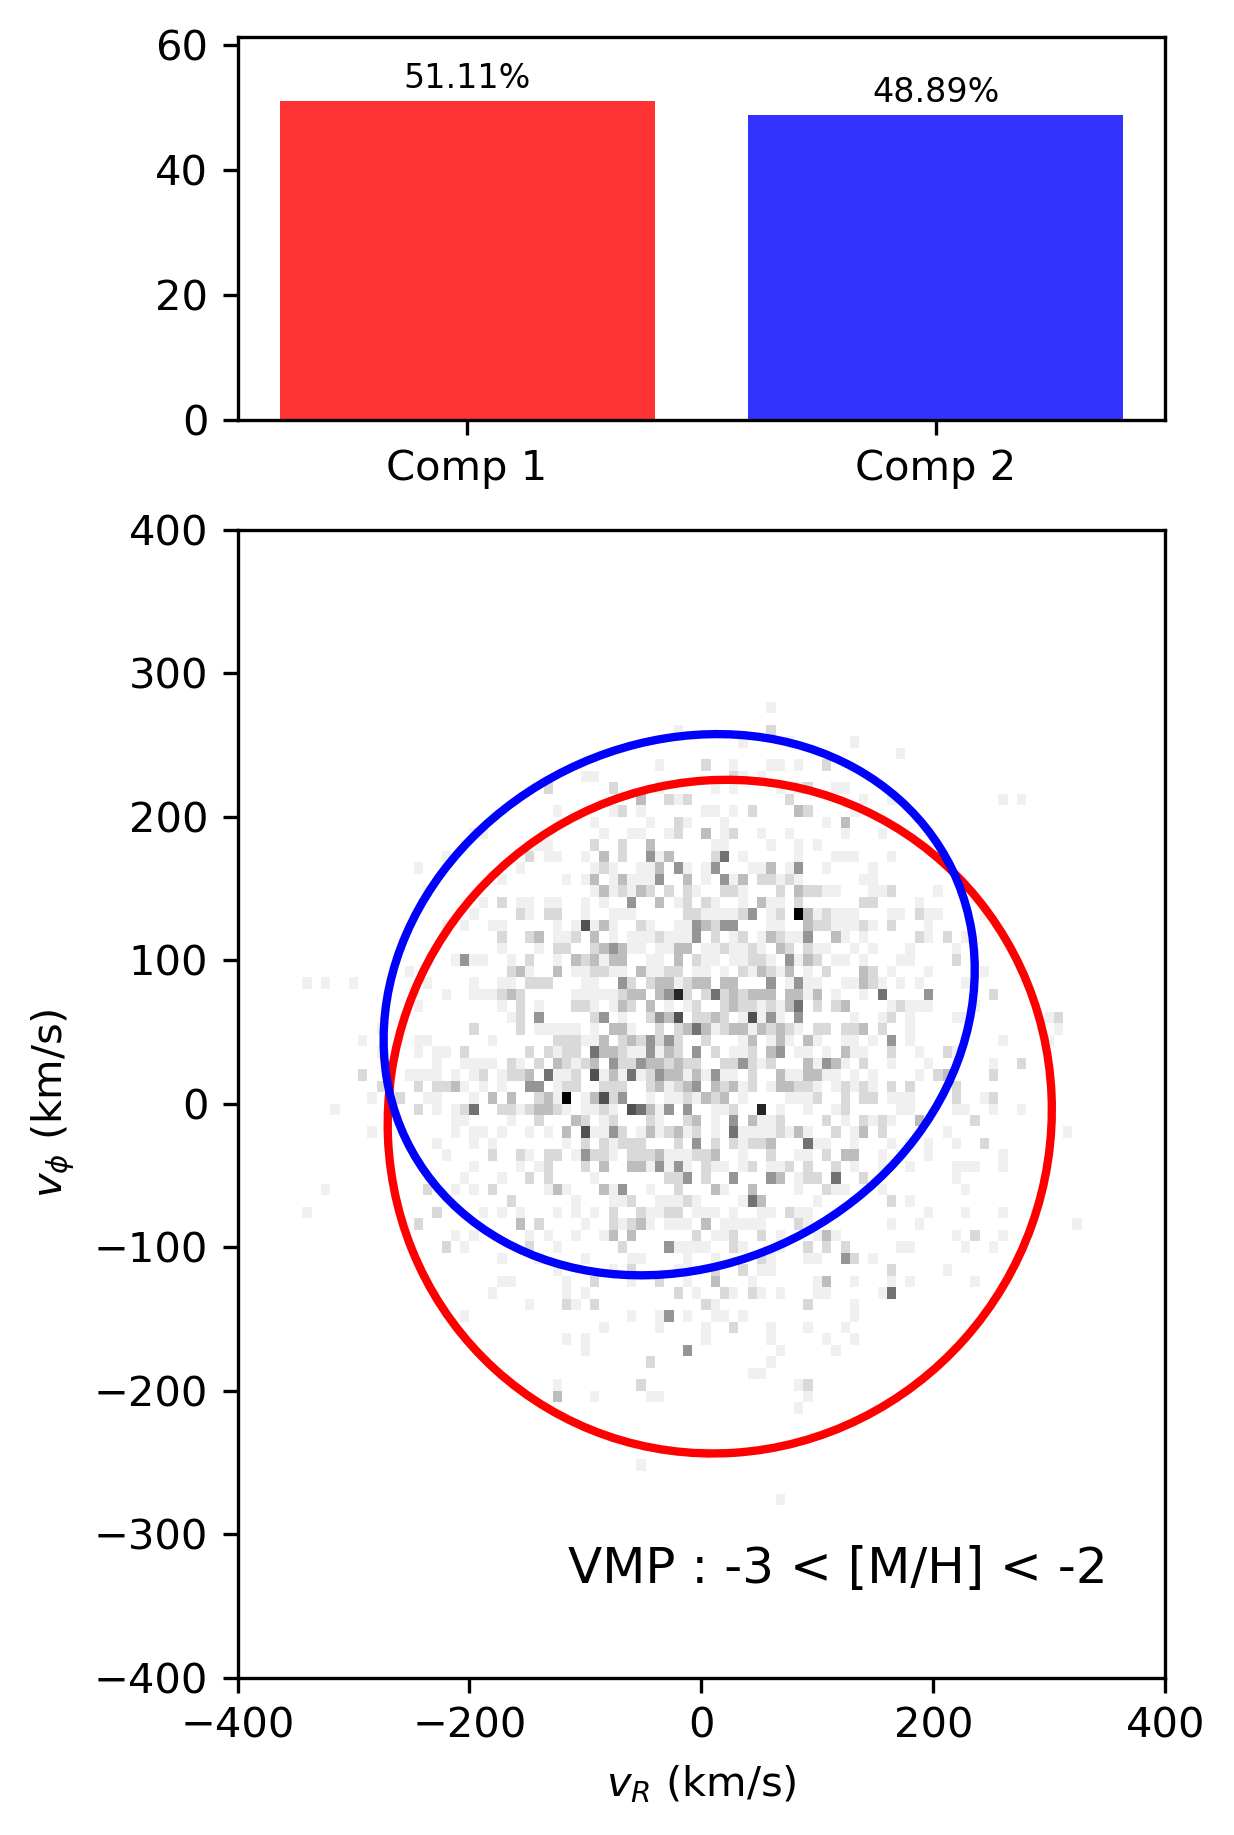
\includegraphics[width=\linewidth]{../figures/gmm_VMP.png}
        \caption{\href{https://raw.githack.com/raunaq-rai/Disentangling-the-Milky-Way-using-GMM/main/figures/VMP\_\_-3\%5BM\_H\%5D-2.html}{VMP}}
        \label{fig:gmm_vmp}
    \end{subfigure}\hfill
    \begin{subfigure}[t]{0.24\textwidth}
        \centering
        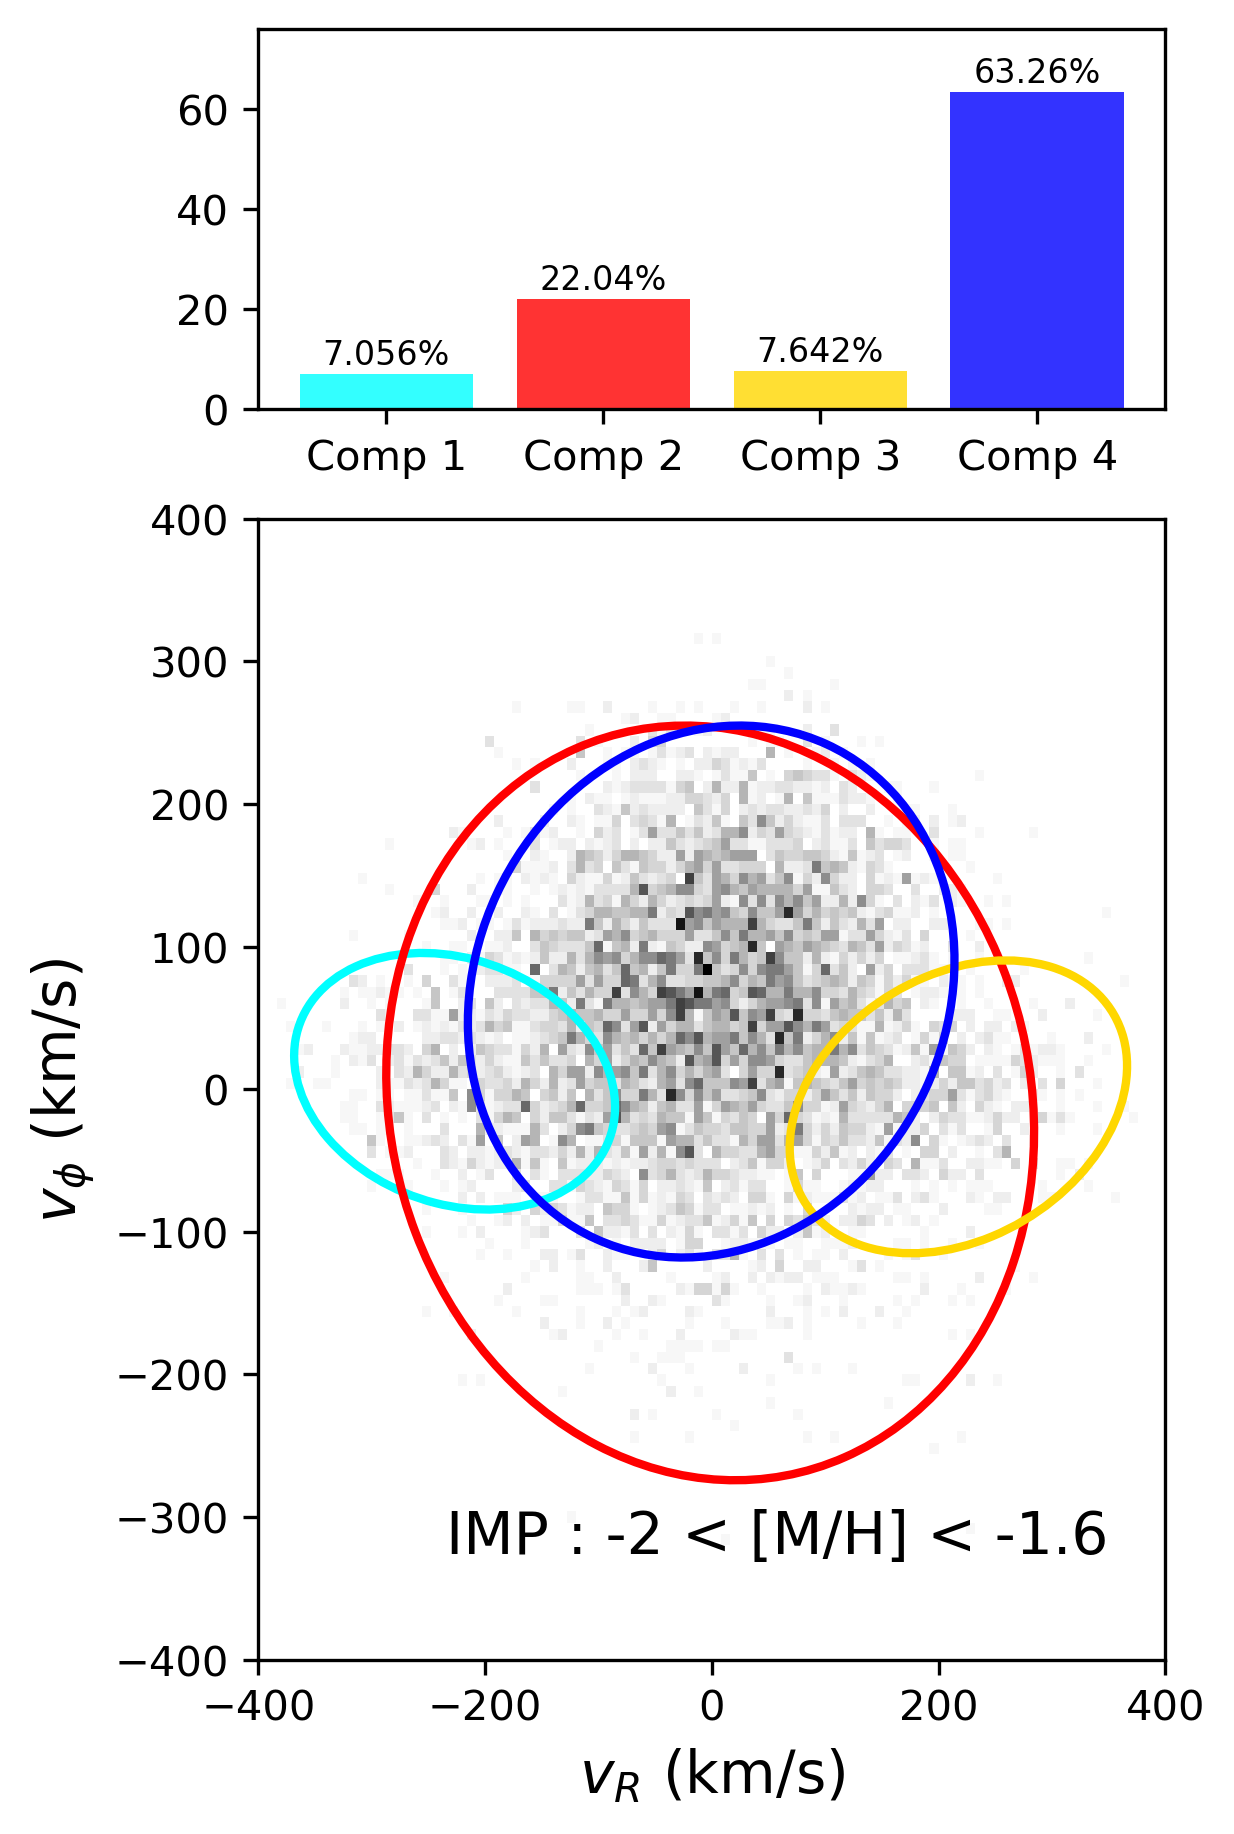
\includegraphics[width=\linewidth]{../figures/gmm_IMP.png}
        \caption{\href{https://raw.githack.com/raunaq-rai/Disentangling-the-Milky-Way-using-GMM/main/figures/IMP\_\_-2\%5BM\_H\%5D-1.6.html}{IMP}}
        \label{fig:gmm_imp}
    \end{subfigure}\hfill
    \begin{subfigure}[t]{0.24\textwidth}
        \centering
        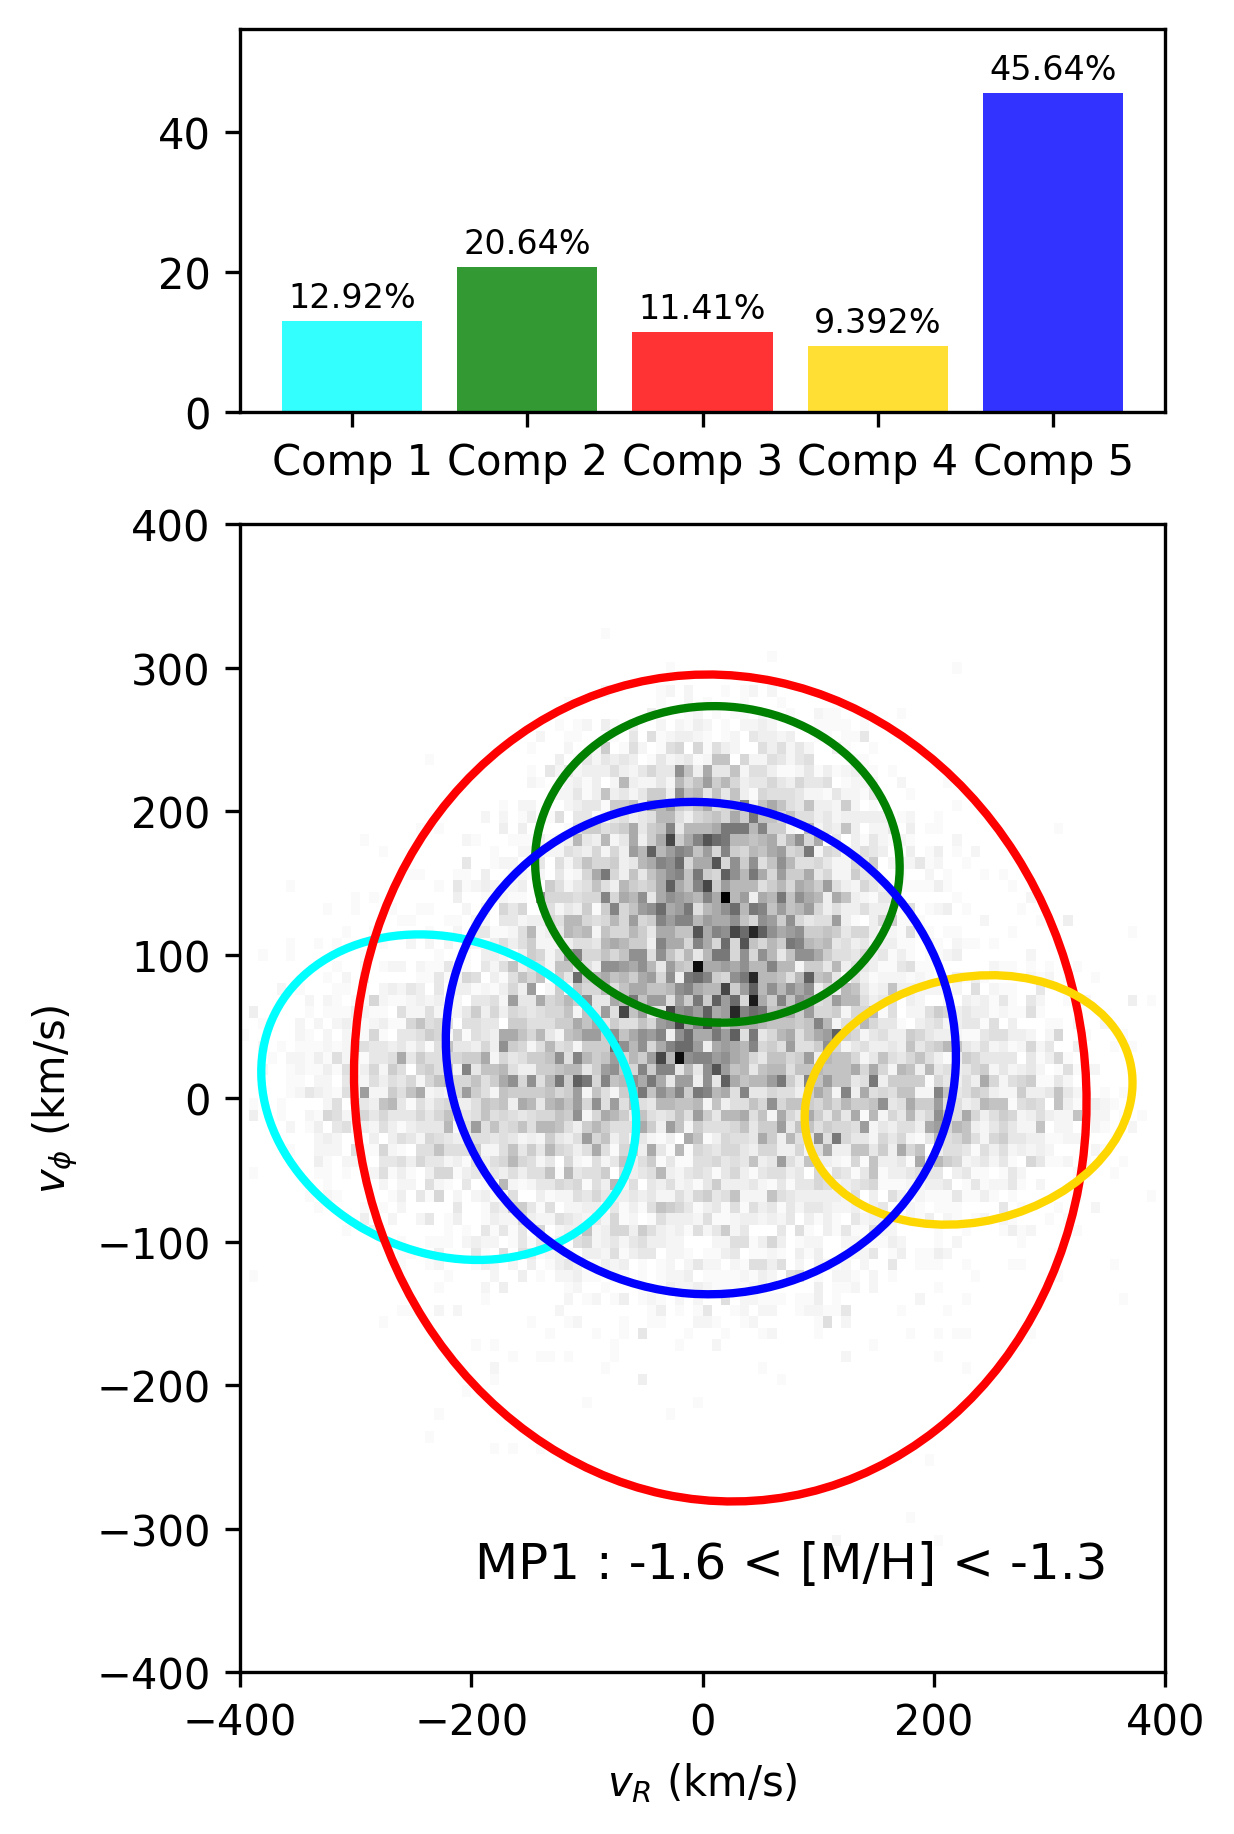
\includegraphics[width=\linewidth]{../figures/gmm_MP1.png}
        \caption{\href{https://raw.githack.com/raunaq-rai/Disentangling-the-Milky-Way-using-GMM/main/figures/MP1\_\_-1.6\%5BM\_H\%5D-1.3.html}{MP1}}
        \label{fig:gmm_mp1}
    \end{subfigure}\hfill
    \begin{subfigure}[t]{0.24\textwidth}
        \centering
        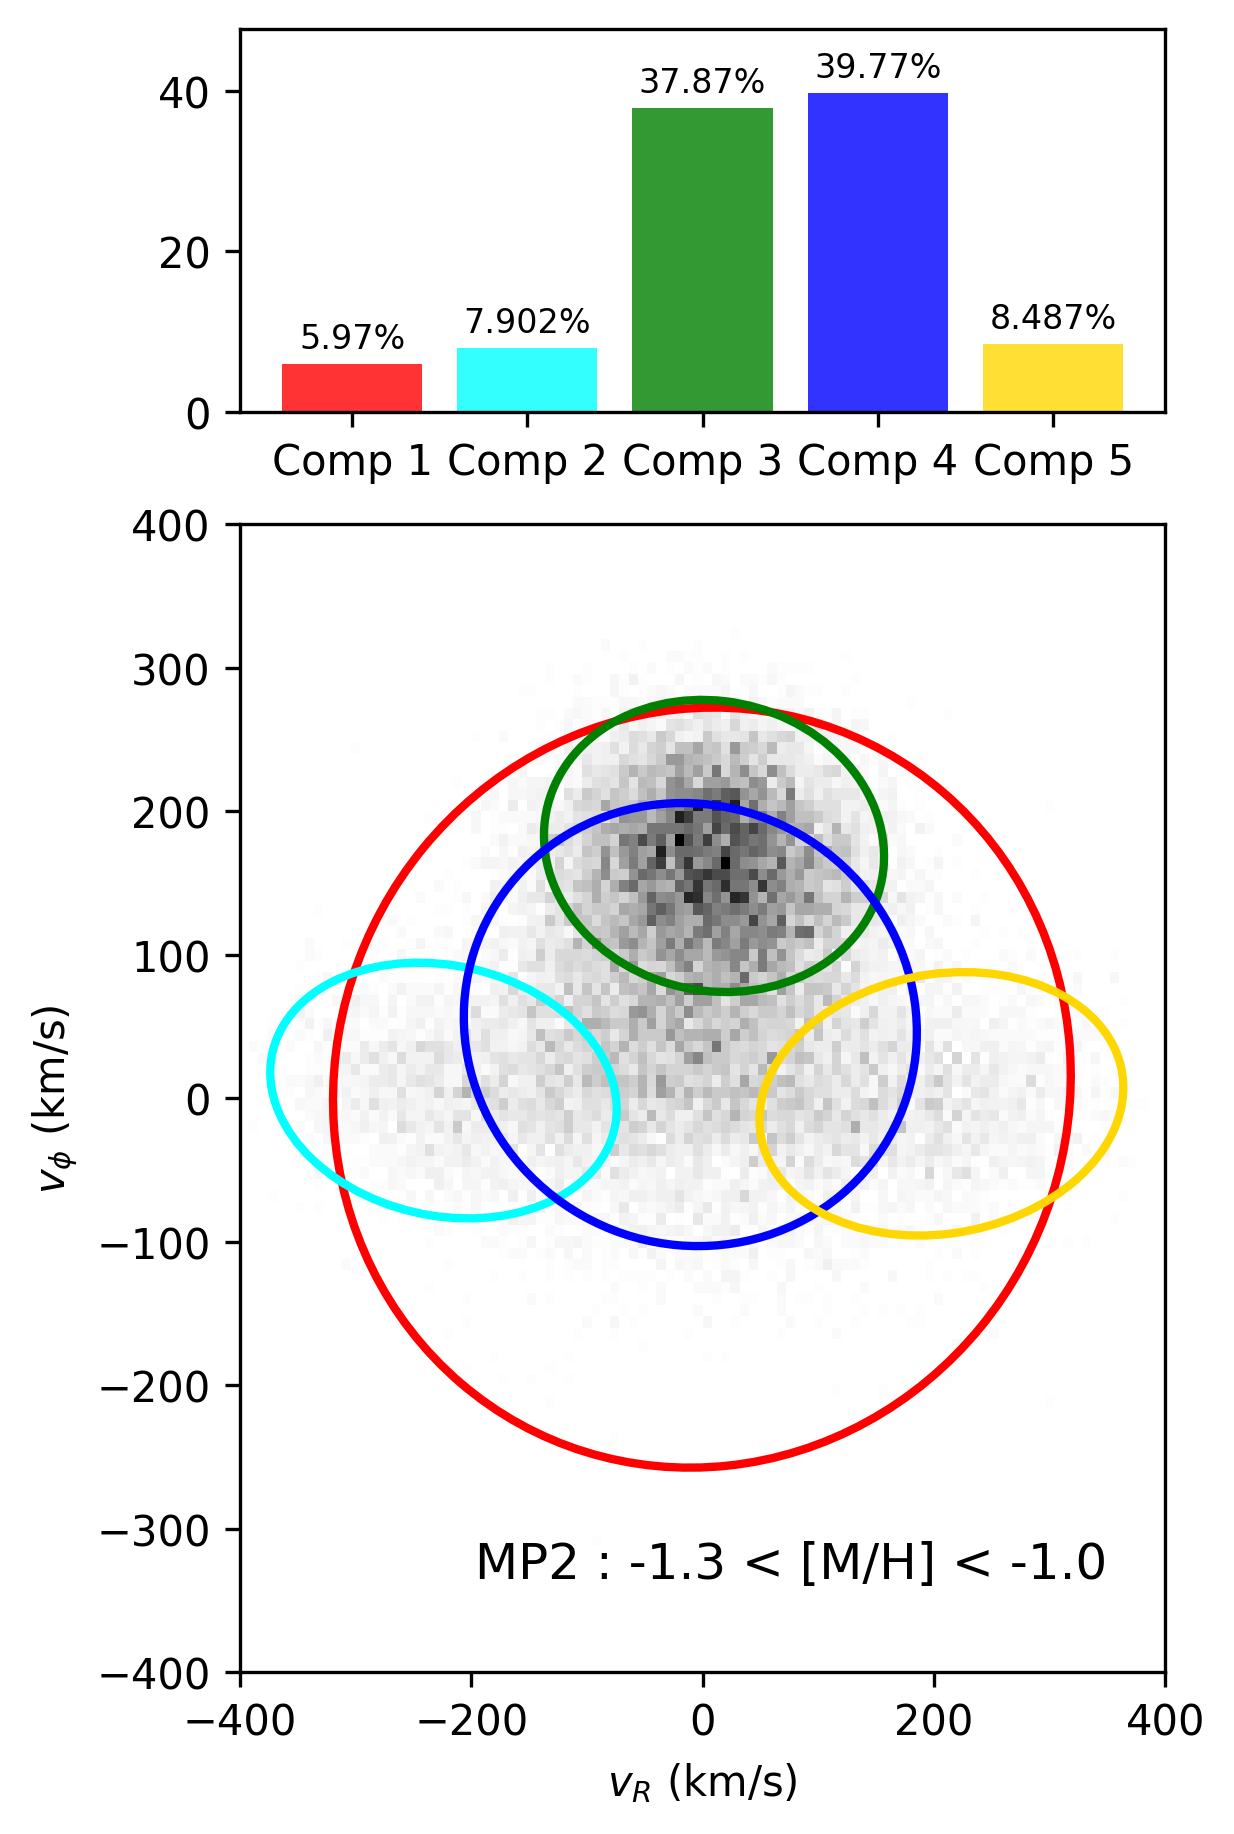
\includegraphics[width=\linewidth]{../figures/gmm_MP2.png}
        \caption{\href{https://raw.githack.com/raunaq-rai/Disentangling-the-Milky-Way-using-GMM/main/figures/MP2\_\_-1.3\%5BM\_H\%5D-1.0.html}{MP2}}
        \label{fig:gmm_mp2}
    \end{subfigure}
    
    \caption{
        Gaussian Mixture Model decompositions of the stellar velocity distribution in the $v_R$–$v_\phi$ plane for each metallicity bin. 
        The lower panels show the 2D $v_R$–$v_\phi$ distributions with GMM components overplotted as 1$\sigma$ ellipses, and the upper panels display each component’s fractional contribution. 
        (Reproduced from \citealt{zhang2024existencemetalpoordiscmilky} Figure~5.)  
        Links to the fully interactive 3-D plots for each bin are provided as hyperlinks in the subcaptions.
    }
    \label{fig:gmm_decompositions}
\end{figure*}

As shown in Figure~\ref{fig:gmm_decompositions}, the GMM is able to capture kinematic substructures in the velocity space 
of metal-poor stars. As metalicity increases, a gaussian component with a clear prograde rotation signal emerges (in green),
indiciative of a disc-like structure. The statistics of the GMM fit are summarised in Table~\ref{tab:gmm_parameters},
which lists the weights, means, and dispersions of each component in the four metallicity bins. 


At $\mathrm{[M/H]} < -1.6$ (the VMP and IMP regimes), a disc component is not observed. Instead, the kinematic structure 
is dominated by a prograde halo and a stationary halo. In the VMP bin, the sample is almost evenly split between these 
two components, with the stationary halo contributing 51.1\% and the prograde halo 48.9\%. Both show broad velocity 
dispersions, with only modest rotational support ($\overline{v_\phi} \sim 69$ km\,s$^{-1}$ for the prograde halo) 
and no evidence for a kinematically cold disc-like structure.

In the IMP bin, the picture remains similar, although the prograde halo dominates more strongly 
(63.3\%) and additional substructure becomes apparent. Two minor components, interpreted as fragments of the 
GS/E merger debris, are also identified, each contributing $\sim$7\% of the population 
and exhibiting highly radial orbits ($|v_R| > 200$ km\,s$^{-1}$). These GS/E components are characterised by 
strong anisotropy and contribute to the broadening of the halo distribution, but again show no signature of 
disc-like kinematics. The absence of a cold, rotating disc in these bins suggests that if a very-metal-poor 
disc exists, it must be a minor contributor to the local stellar population.

Our GMM decomposition recovers the same substructures identified by \citet{zhang2024existencemetalpoordiscmilky} 
across all metallicity bins. We find similar velocity dispersions and centroid trends for the stationary halo, 
prograde halo, and GS/E components. Notably, our model assigns a more comparable weight to the 
prograde halo component in the VMP bin, in contrast to the dominant stationary 
halo reported by \citet{zhang2024existencemetalpoordiscmilky}. We also observe some variation 
in the centroid $v_\phi$ values of GS/E substructures, although their bimodal spatial structure is preserved. 

\begin{table*}
\centering
\begin{tabular}{lccccccc}
\hline
\textbf{Components} & \textbf{Weights (\%)} & $\mathbf{v_R}$ & $\boldsymbol{\sigma_R}$ & $\mathbf{v_\phi}$ & $\boldsymbol{\sigma_\phi}$ & $\mathbf{v_Z}$ & $\boldsymbol{\sigma_Z}$ \\
\hline
\multicolumn{8}{l}{\textbf{VMP:} $-3.0 < \mathrm{[M/H]} < -2.0$ (4768 stars)} \\
Stationary halo     & 51.1 & 15.86   & 143.17 &  -9.13  & 117.36 & -0.08 & 122.64 \\
Prograde halo       & 48.9 & -19.14  & 127.43 &  68.86  &  94.28 & -0.90 &  82.89 \\
\hline
\multicolumn{8}{l}{\textbf{IMP:} $-2.0 < \mathrm{[M/H]} < -1.6$ (12052 stars)} \\
Stationary halo     & 22.0 &  -1.45  & 142.88 &  -9.59  & 132.32 & -0.91 & 124.92 \\
Prograde halo       & 63.3 &  -0.58  & 107.32 &  68.52  &  93.27 & -1.16 &  72.56 \\
GS/E(1)             &  7.1 & -226.92 &  70.78 &   5.60  &  44.98 &  8.43 &  88.40 \\
GS/E(2)             &  7.6 &  217.52 &  74.41 & -12.35  &  51.35 & -4.22 &  89.78 \\
\hline
\multicolumn{8}{l}{\textbf{MP1:} $-1.6 < \mathrm{[M/H]} < -1.3$ (19142 stars)} \\
Stationary halo     & 11.3 &  15.09  & 158.68 &   7.11  & 144.33 & -2.55 & 132.08 \\
Prograde halo       & 44.5 &  -3.02  & 111.54 &  31.79  &  85.15 & -0.54 &  70.36 \\
GS/E(1)             & 12.7 & -220.40 &  80.76 &   1.01  &  56.29 &  0.47 &  91.00 \\
GS/E(2)             &  9.4 &  229.32 &  71.22 &  -0.82  &  43.42 &  1.42 &  92.69 \\
Thick disc          & 22.1 &  12.93  &  79.56 & 160.32  &  56.58 & -2.31 &  68.83 \\
\hline
\multicolumn{8}{l}{\textbf{MP2:} $-1.3 < \mathrm{[M/H]} < -1.0$ (30892 stars)} \\
Stationary halo     &  6.1 &  -1.17  & 159.06 &   8.07  & 132.05 & -3.37 & 120.46 \\
Prograde halo       & 39.4 & -13.47  &  95.65 &  53.64  &  77.86 & -3.04 &  71.00 \\
GS/E(1)             &  7.9 & -224.68 &  74.44 &   5.73  &  44.63 &  2.41 &  87.27 \\
GS/E(2)             &  9.3 &  199.71 &  81.28 &  -3.30  &  46.84 & -2.07 &  88.99 \\
Thick disc          & 37.4 &  10.56  &  73.55 & 176.07  &  50.79 &  0.85 &  62.03 \\
\hline
\end{tabular}
\caption{Parameters of the Gaussian mixture model fittings in different metallicity bins.
 The unit for all velocity columns is km\,s$^{-1}$.}
\label{tab:gmm_parameters}
\end{table*}

\subsection{Rotational Support and the Onset of Disc Formation}

To assess the degree of rotational support in each component, we compute the ratio 
$V_{\rm rot} / \sigma_\phi$, where $V_{\rm rot}$ is the mean azimuthal velocity and 
$\sigma_\phi$ its dispersion. This ratio serves as a conventional diagnostic of disc-like 
kinematics, with values $\gtrsim 3$ indicating rotation-supported populations. As shown in 
Figure~\ref{fig:v_over_sigma}, all components in the VMP and IMP bins fall below this threshold, 
confirming that the GMM identifies only dynamically hot, dispersion-supported structures in these 
regimes.

At higher metallicities, a dynamically colder disc population emerges. In the MP1 bin, the thick 
disc component (green) rotates at $v_\phi \sim 160$ km\,s$^{-1}$ with $\sigma_\phi \sim 57$ km\,s$^{-1}$, 
yielding $V_{\rm rot} / \sigma_\phi \approx 2.8$. While just below the canonical boundary, this 
component’s low vertical dispersion and substantial weight (22.1\%) mark it as a distinct disc-like 
structure. By the MP2 bin, the disc becomes the dominant component (37.4\%), with 
$V_{\rm rot} / \sigma_\phi \approx 3.5$, indicating clear rotational support and a well-established 
thick disc. These trends suggest a transition in the stellar kinematics around 
$\mathrm{[M/H]} \sim -1.5$.

Meanwhile, the GS/E components (identifiable in the IMP, MP1, and MP2 bins) remain dynamically 
distinct, with high $|v_R|$, relatively small $v_\phi$, and negligible rotational support, reinforcing 
their origin as debris from a major radial merger \citep{Helmi2018}. Notably, given 
the estimated time of the GS/E accretion event (of order 8–11 Gyr ago \citep{Gallart2019,Belokurov2020,DiMatteo2019}),its stellar 
debris is expected to be phase-mixed. This 
implies that the positive and negative $v_R$ components should contribute approximately equally. 
This symmetry is observed in the IMP and two MP bins. 


\begin{figure}[H]
    \centering
    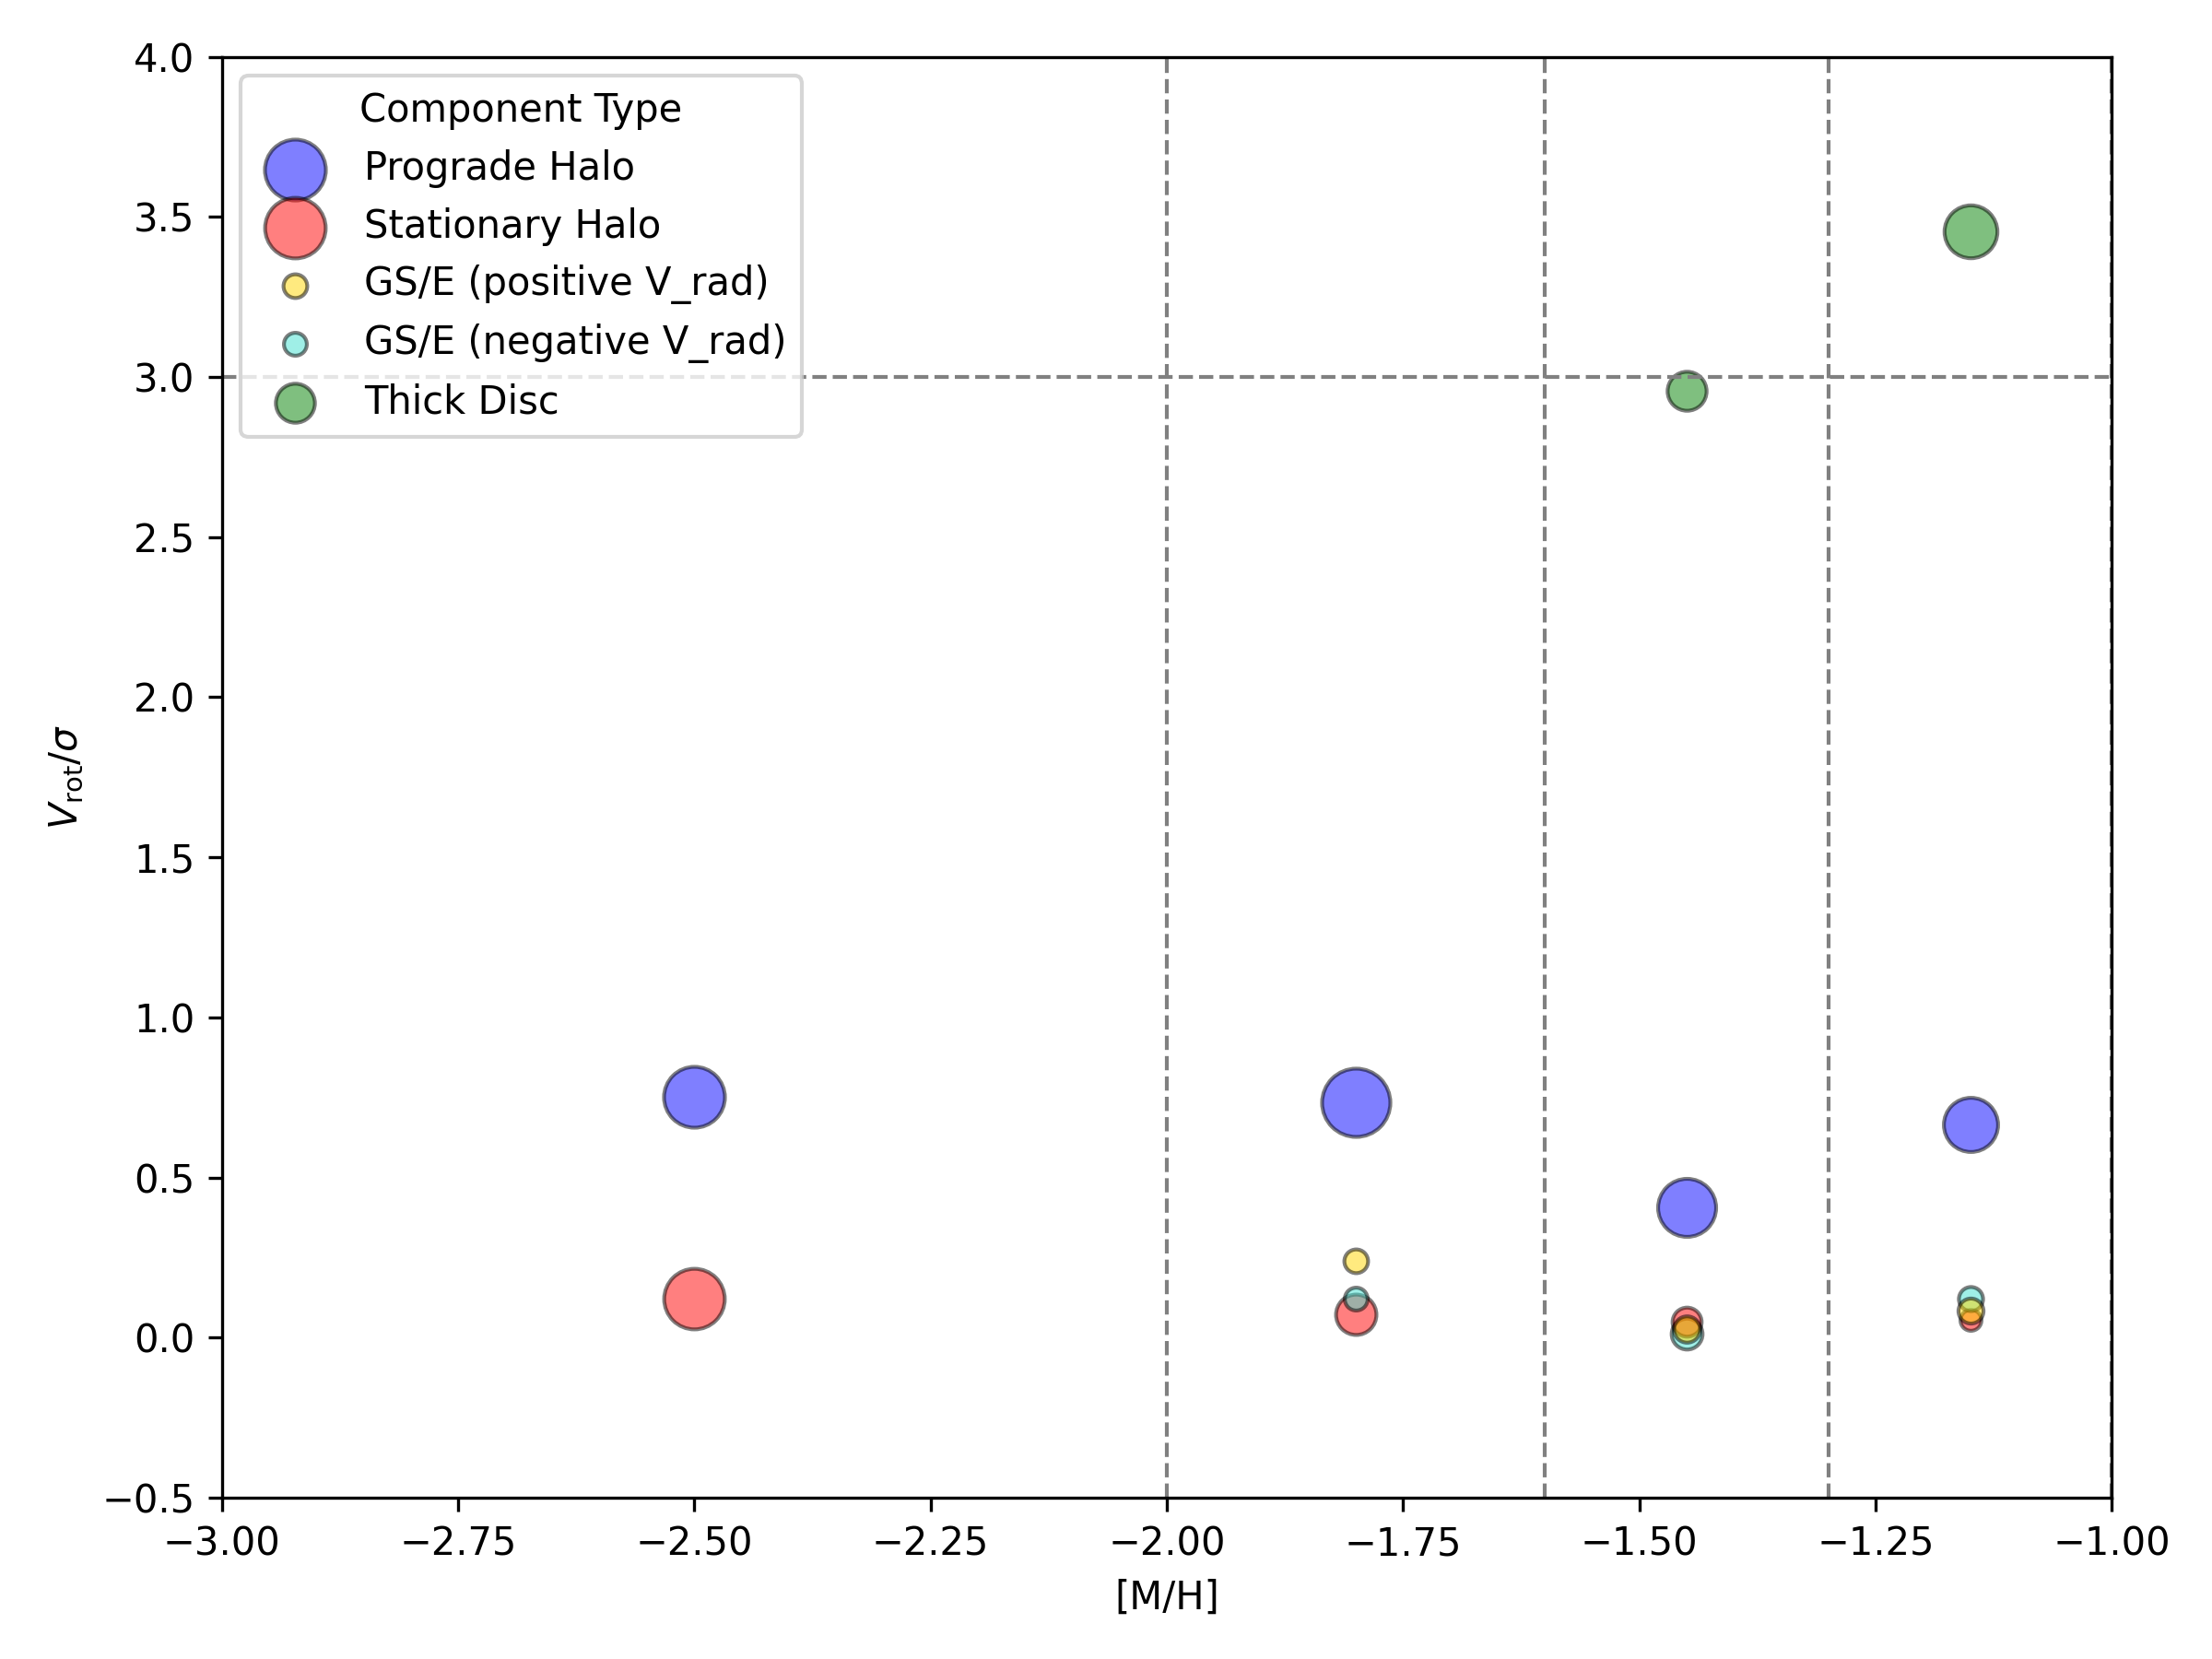
\includegraphics[width=\linewidth]{../figures/v_over_sigma_per_component.png}
    \caption{Ratio of mean rotational velocity to azimuthal velocity dispersion, 
    $V_{\rm rot} / \sigma_\phi$, for individual GMM components in each metallicity bin. 
    Larger circles correspond to more dominant components. Colours match the GMM components 
    in Figure~\ref{fig:gmm_decompositions}.(A reproduction of Figure 6 from \citet{zhang2024existencemetalpoordiscmilky})}
    \label{fig:v_over_sigma}
\end{figure}

\subsection{Residual Analysis for Hidden Disc Populations}

One of the limitations of GMMs is that they can fail to detect substructures that contribute 
only weakly to the overall distribution. To investigate this, we performed a residual analysis to test 
whether a disc-like population, too weak to be picked up by the GMM, might be present 
in the VMP and IMP metallicity regimes.

Following \citet{zhang2024existencemetalpoordiscmilky}, we generated a synthetic dataset by drawing 
the same number of mock stars as observed stars from 
the best-fit GMM in each bin. Since our GMM uses the Extreme Deconvolution algorithm, which accounts 
for observational uncertainties during fitting, the raw samples from the model are noise-free. 
However, comparing these directly to real data would be inappropriate due to the absence of measurement 
error. To resolve this, we assign each mock star the velocity uncertainties of its nearest neighbour 
in the observed data (in $(v_R, v_\phi, v_Z)$ space), and then add Gaussian noise according to 
these uncertainties.

We then bin both the observed and mock data in the $(v_R, v_\phi)$ plane and compute the 
normalized residual map, defined as
\[
H_{\mathrm{residual}} = \frac{H_{\mathrm{obs}} - H_{\mathrm{mock}}}{H_{\mathrm{obs}} + H_{\mathrm{mock}} + \epsilon},
\]
where $H_{\mathrm{obs}}$ and $H_{\mathrm{mock}}$ are the 2D histograms and $\epsilon = 10^{-5}$ is added 
to avoid division by zero. The residual maps are shown in the top row of Figure~\ref{fig:residuals} for 
the VMP and IMP bins. The grey dashed ellipses highlight a $2\sigma$ region of a hypothetical thick disc 
with mean velocity $(v_R, v_\phi) = (0, 180)\,\mathrm{km\,s^{-1}}$ and dispersions $(\sigma_R, \sigma_\phi) 
= (70, 50)\,\mathrm{km\,s^{-1}}$, consistent with the thick disc component seen in the MP2 metallicity bin.

To quantify the possible presence of a hidden disc, we count the excess number of observed stars inside 
this thick disc ellipse relative to the GMM-generated sample. We repeat this calculation for 1000 Monte 
Carlo realisations to estimate the residual and its uncertainty. The results are shown as horizontal 
dashed lines in the bottom row of Figure~\ref{fig:residuals}, representing a disc-like residual 
of $38.3 \pm 27.1$ stars in the VMP bin and $78.1 \pm 45.1$ stars in the IMP bin.

To interpret these residuals, we repeat the same procedure but now inject a mock disc population—
generated from the same thick disc Gaussian—into the GMM baseline. By varying the injected disc 
fraction from 0\% to 5\% of the sample and recalculating the residual each time, we construct a 
relationship between disc fraction and expected residual. This is shown as the solid black line in the 
bottom panels of Figure~\ref{fig:residuals}, with the red shaded region indicating the $1\sigma$ 
uncertainty across Monte Carlo trials.

The intersection of the solid and dashed lines could imply a hidden disc fraction 
of up to $\sim1\%$ in the VMP bin and IMP bin. Interestingly, the overlap of these lines in the IMP
bin occurs at a lower percentage. These estimates are indicative only: 
measurement uncertainties, GMM modelling choices, and Gaia-selection cuts mean that the true disc 
contribution in the parent VMP/IMP populations may differ \citep{zhang2024existencemetalpoordiscmilky}.  

\begin{figure}[H]
    \centering
    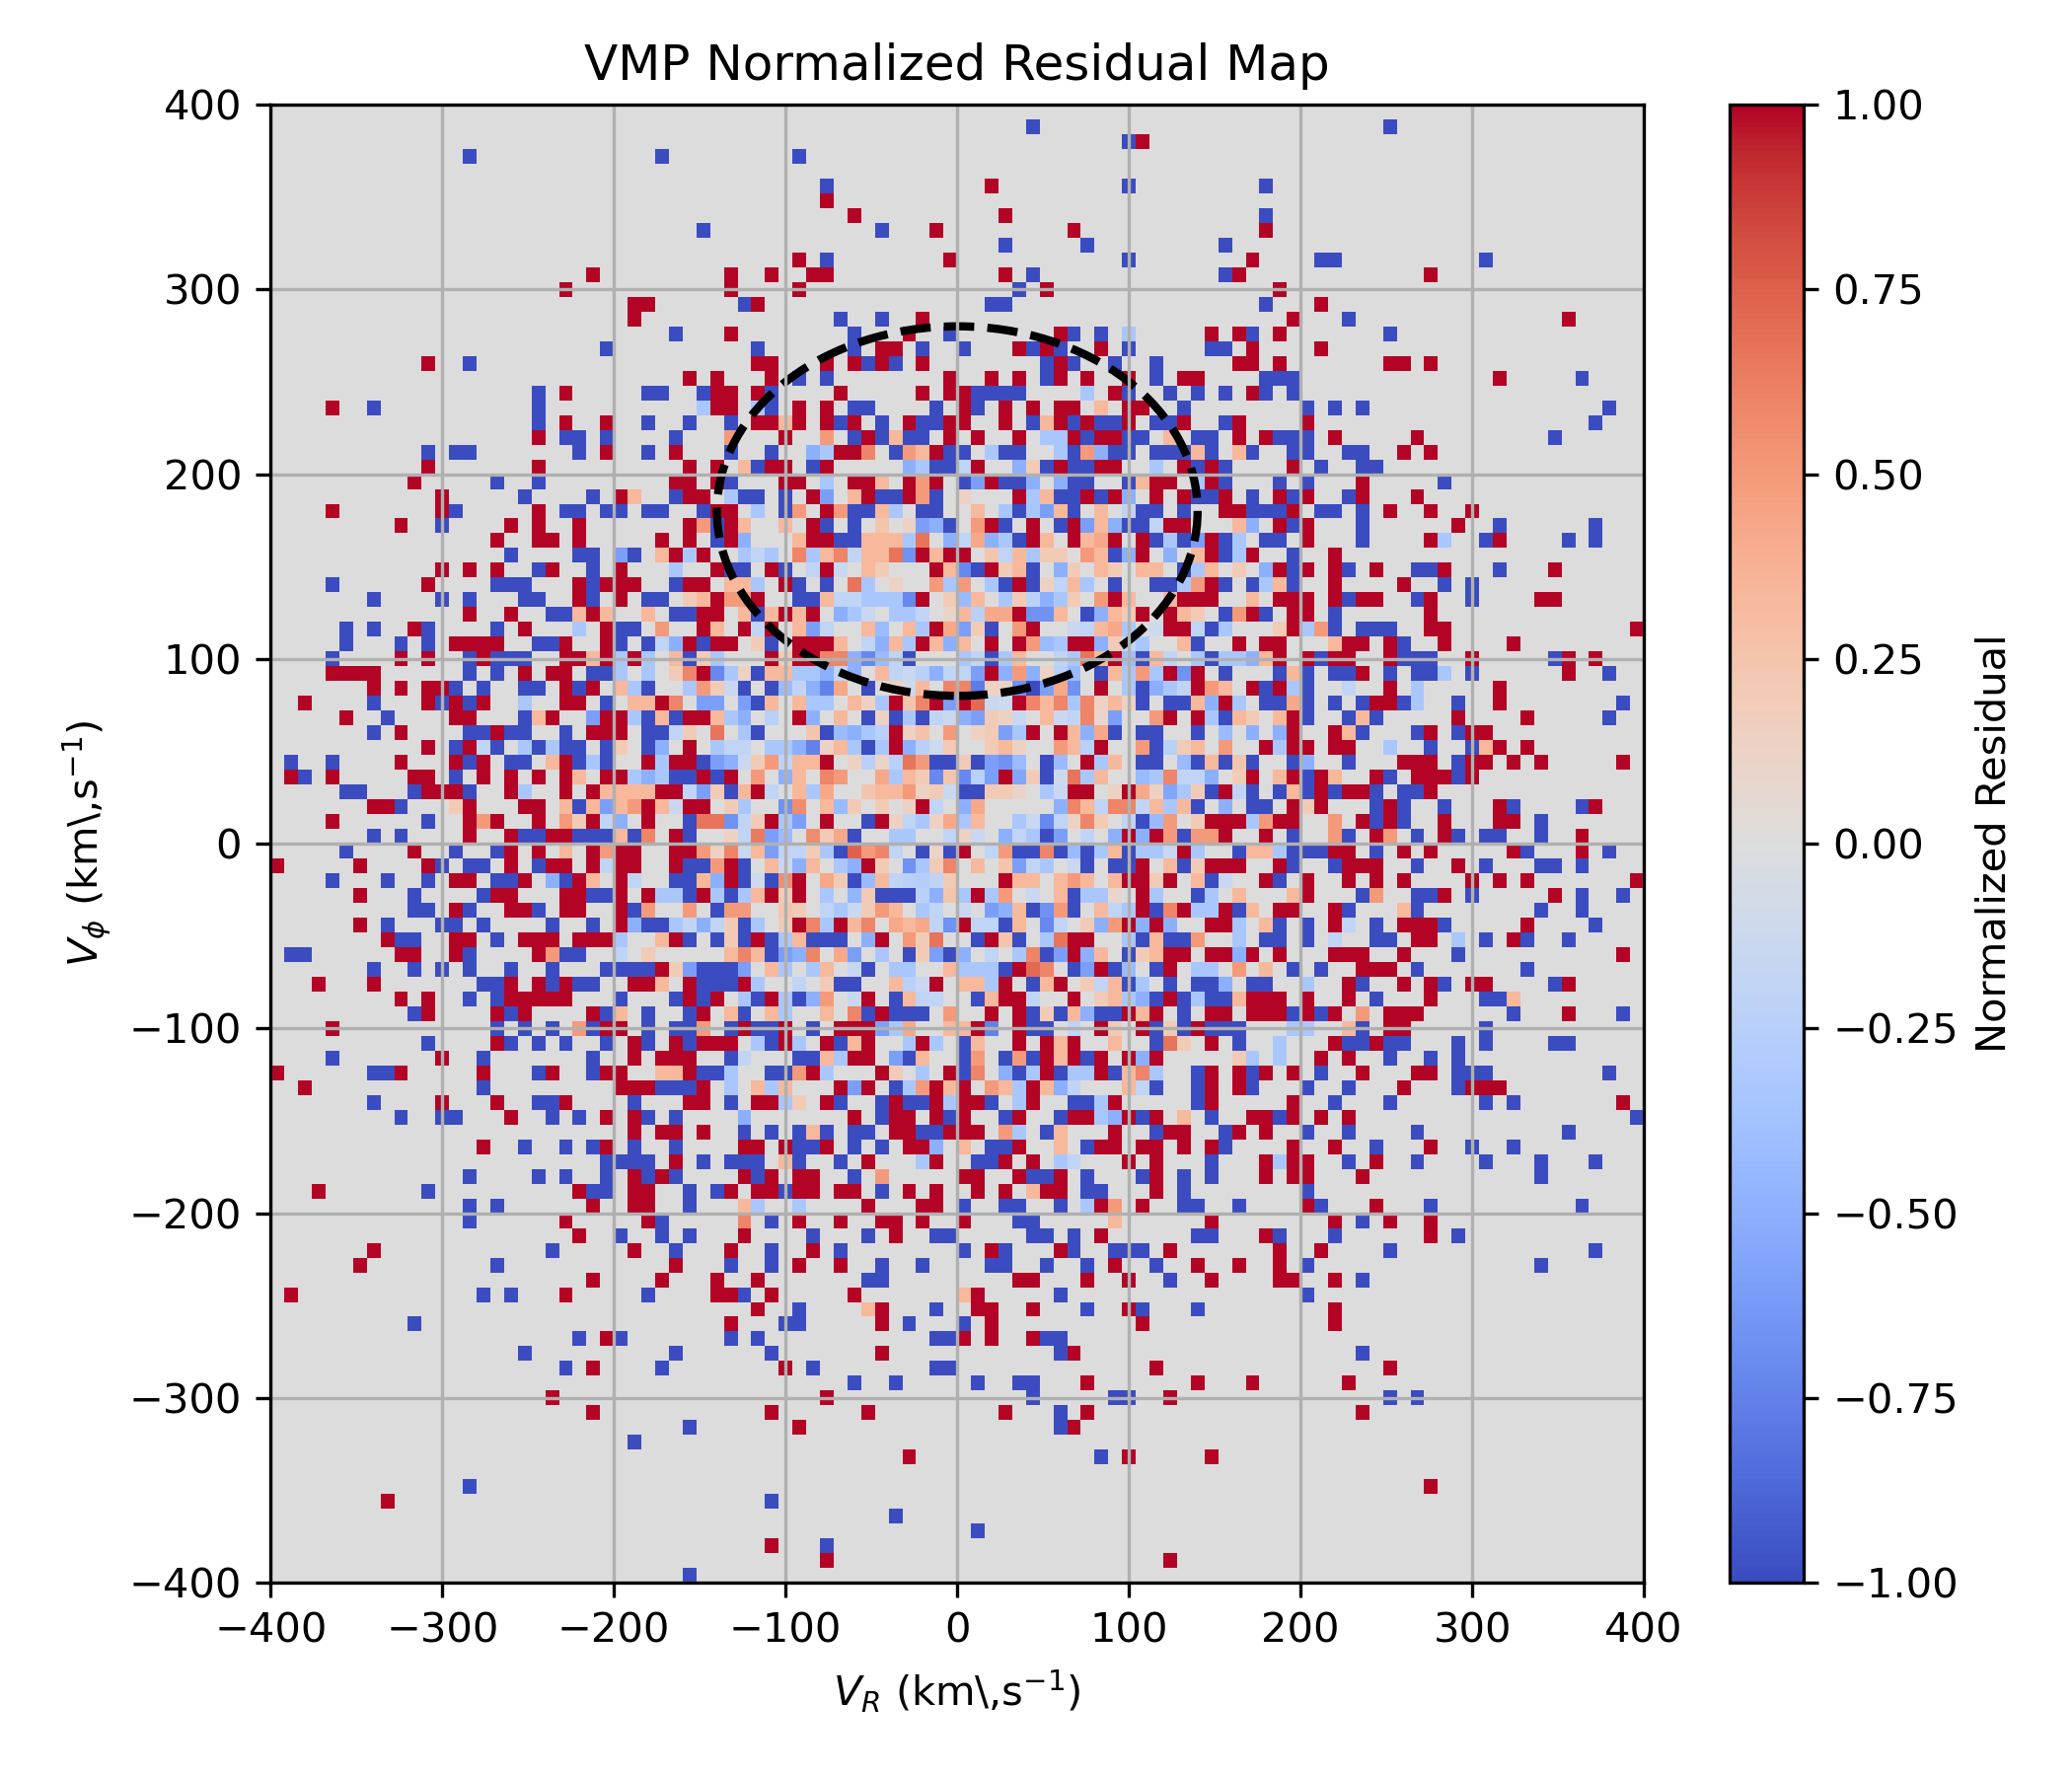
\includegraphics[width=0.49\textwidth]{../figures/vmp_residual_map.png}
    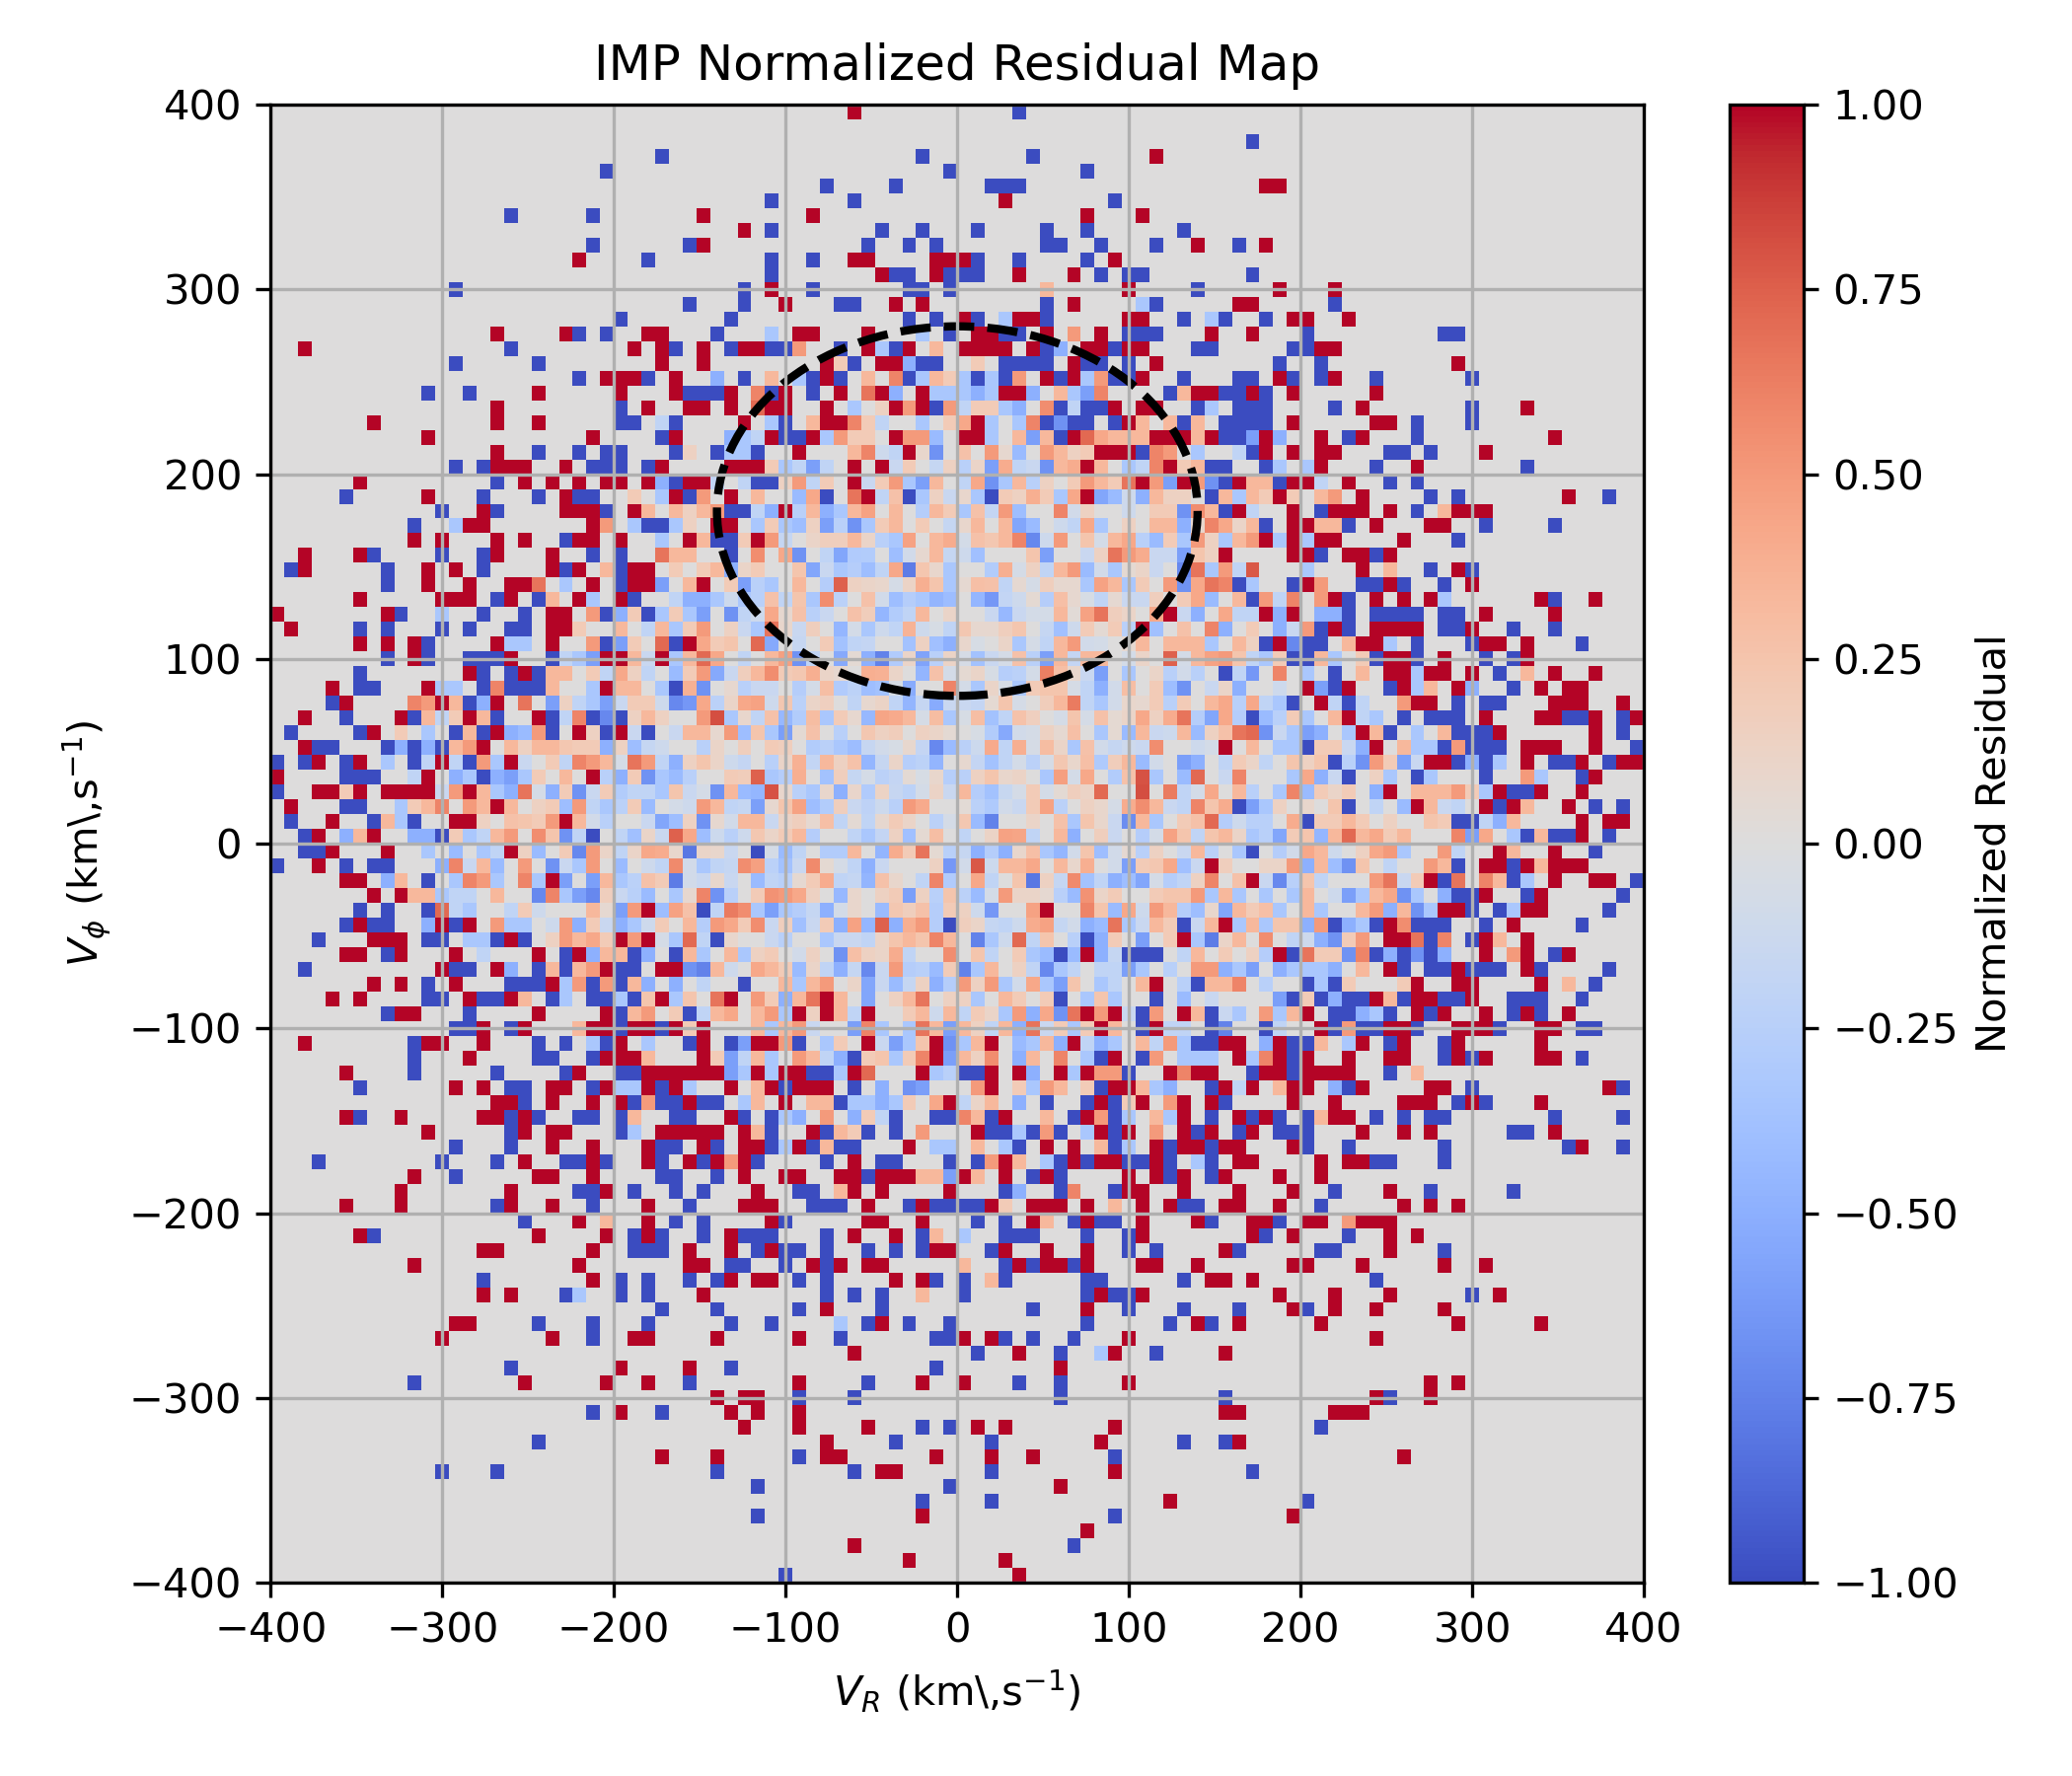
\includegraphics[width=0.49\textwidth]{../figures/imp_residual_map.png} \\
    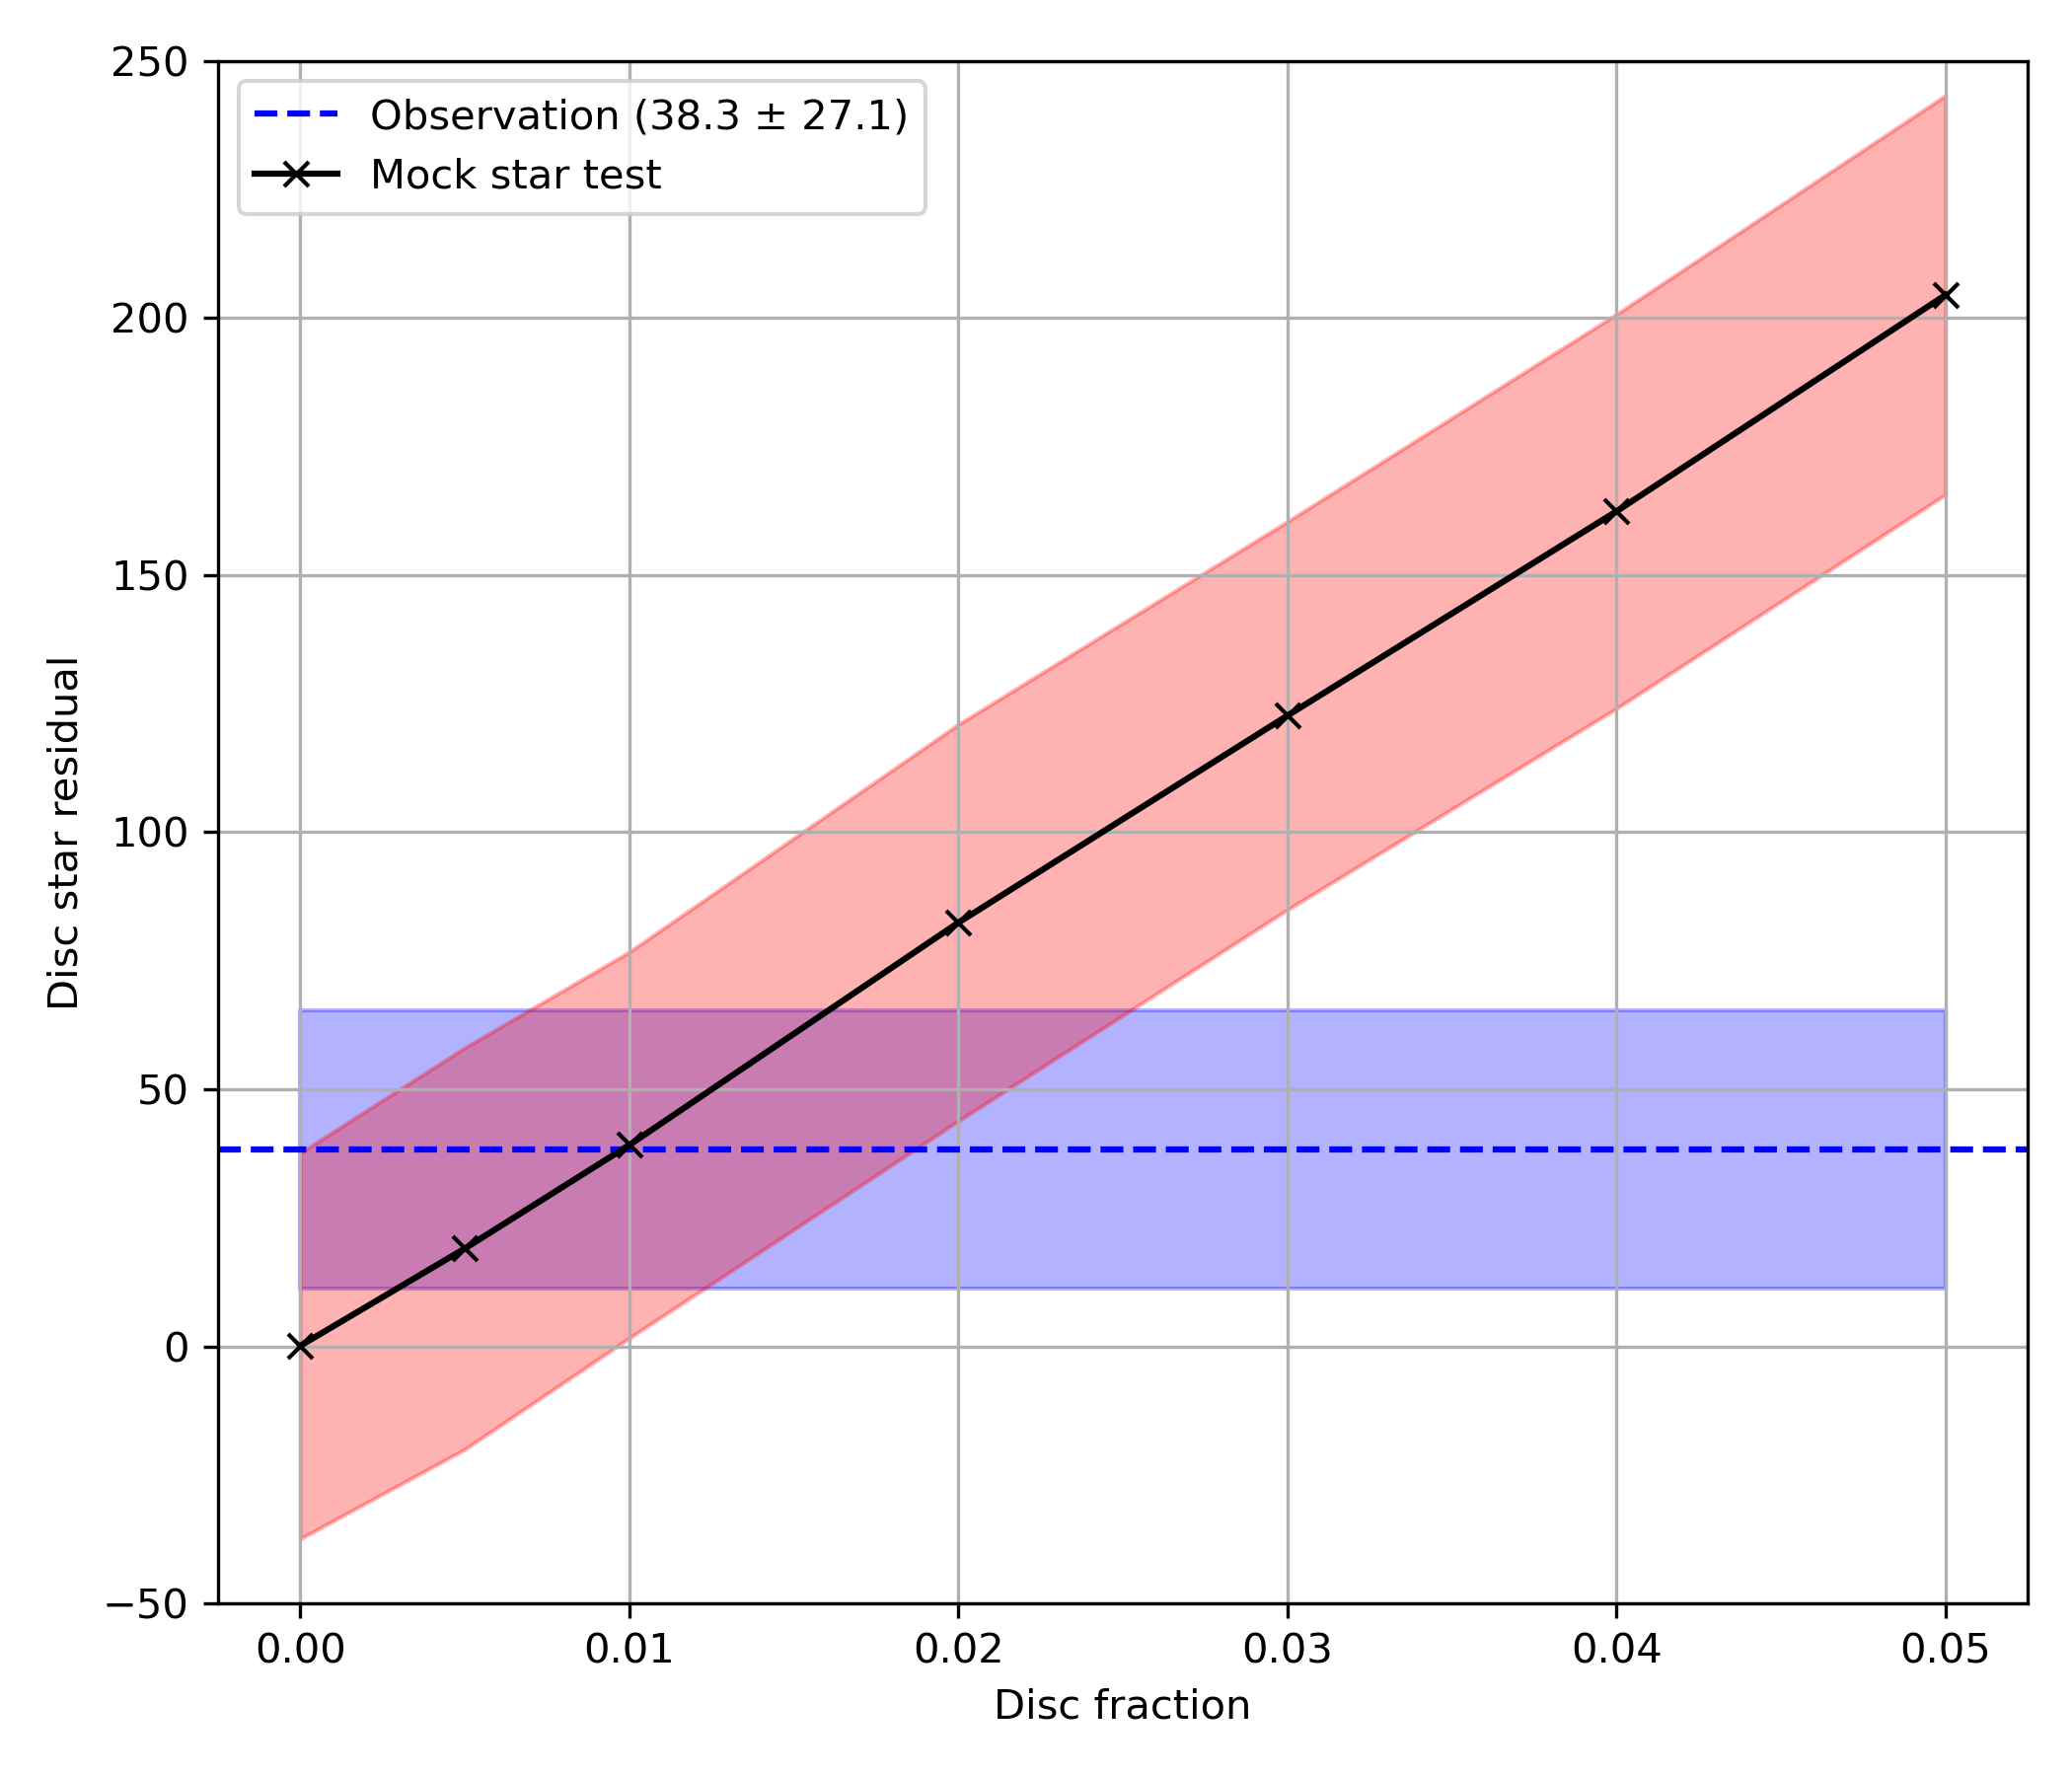
\includegraphics[width=0.49\textwidth]{../figures/vmp_disc_fraction.png}
    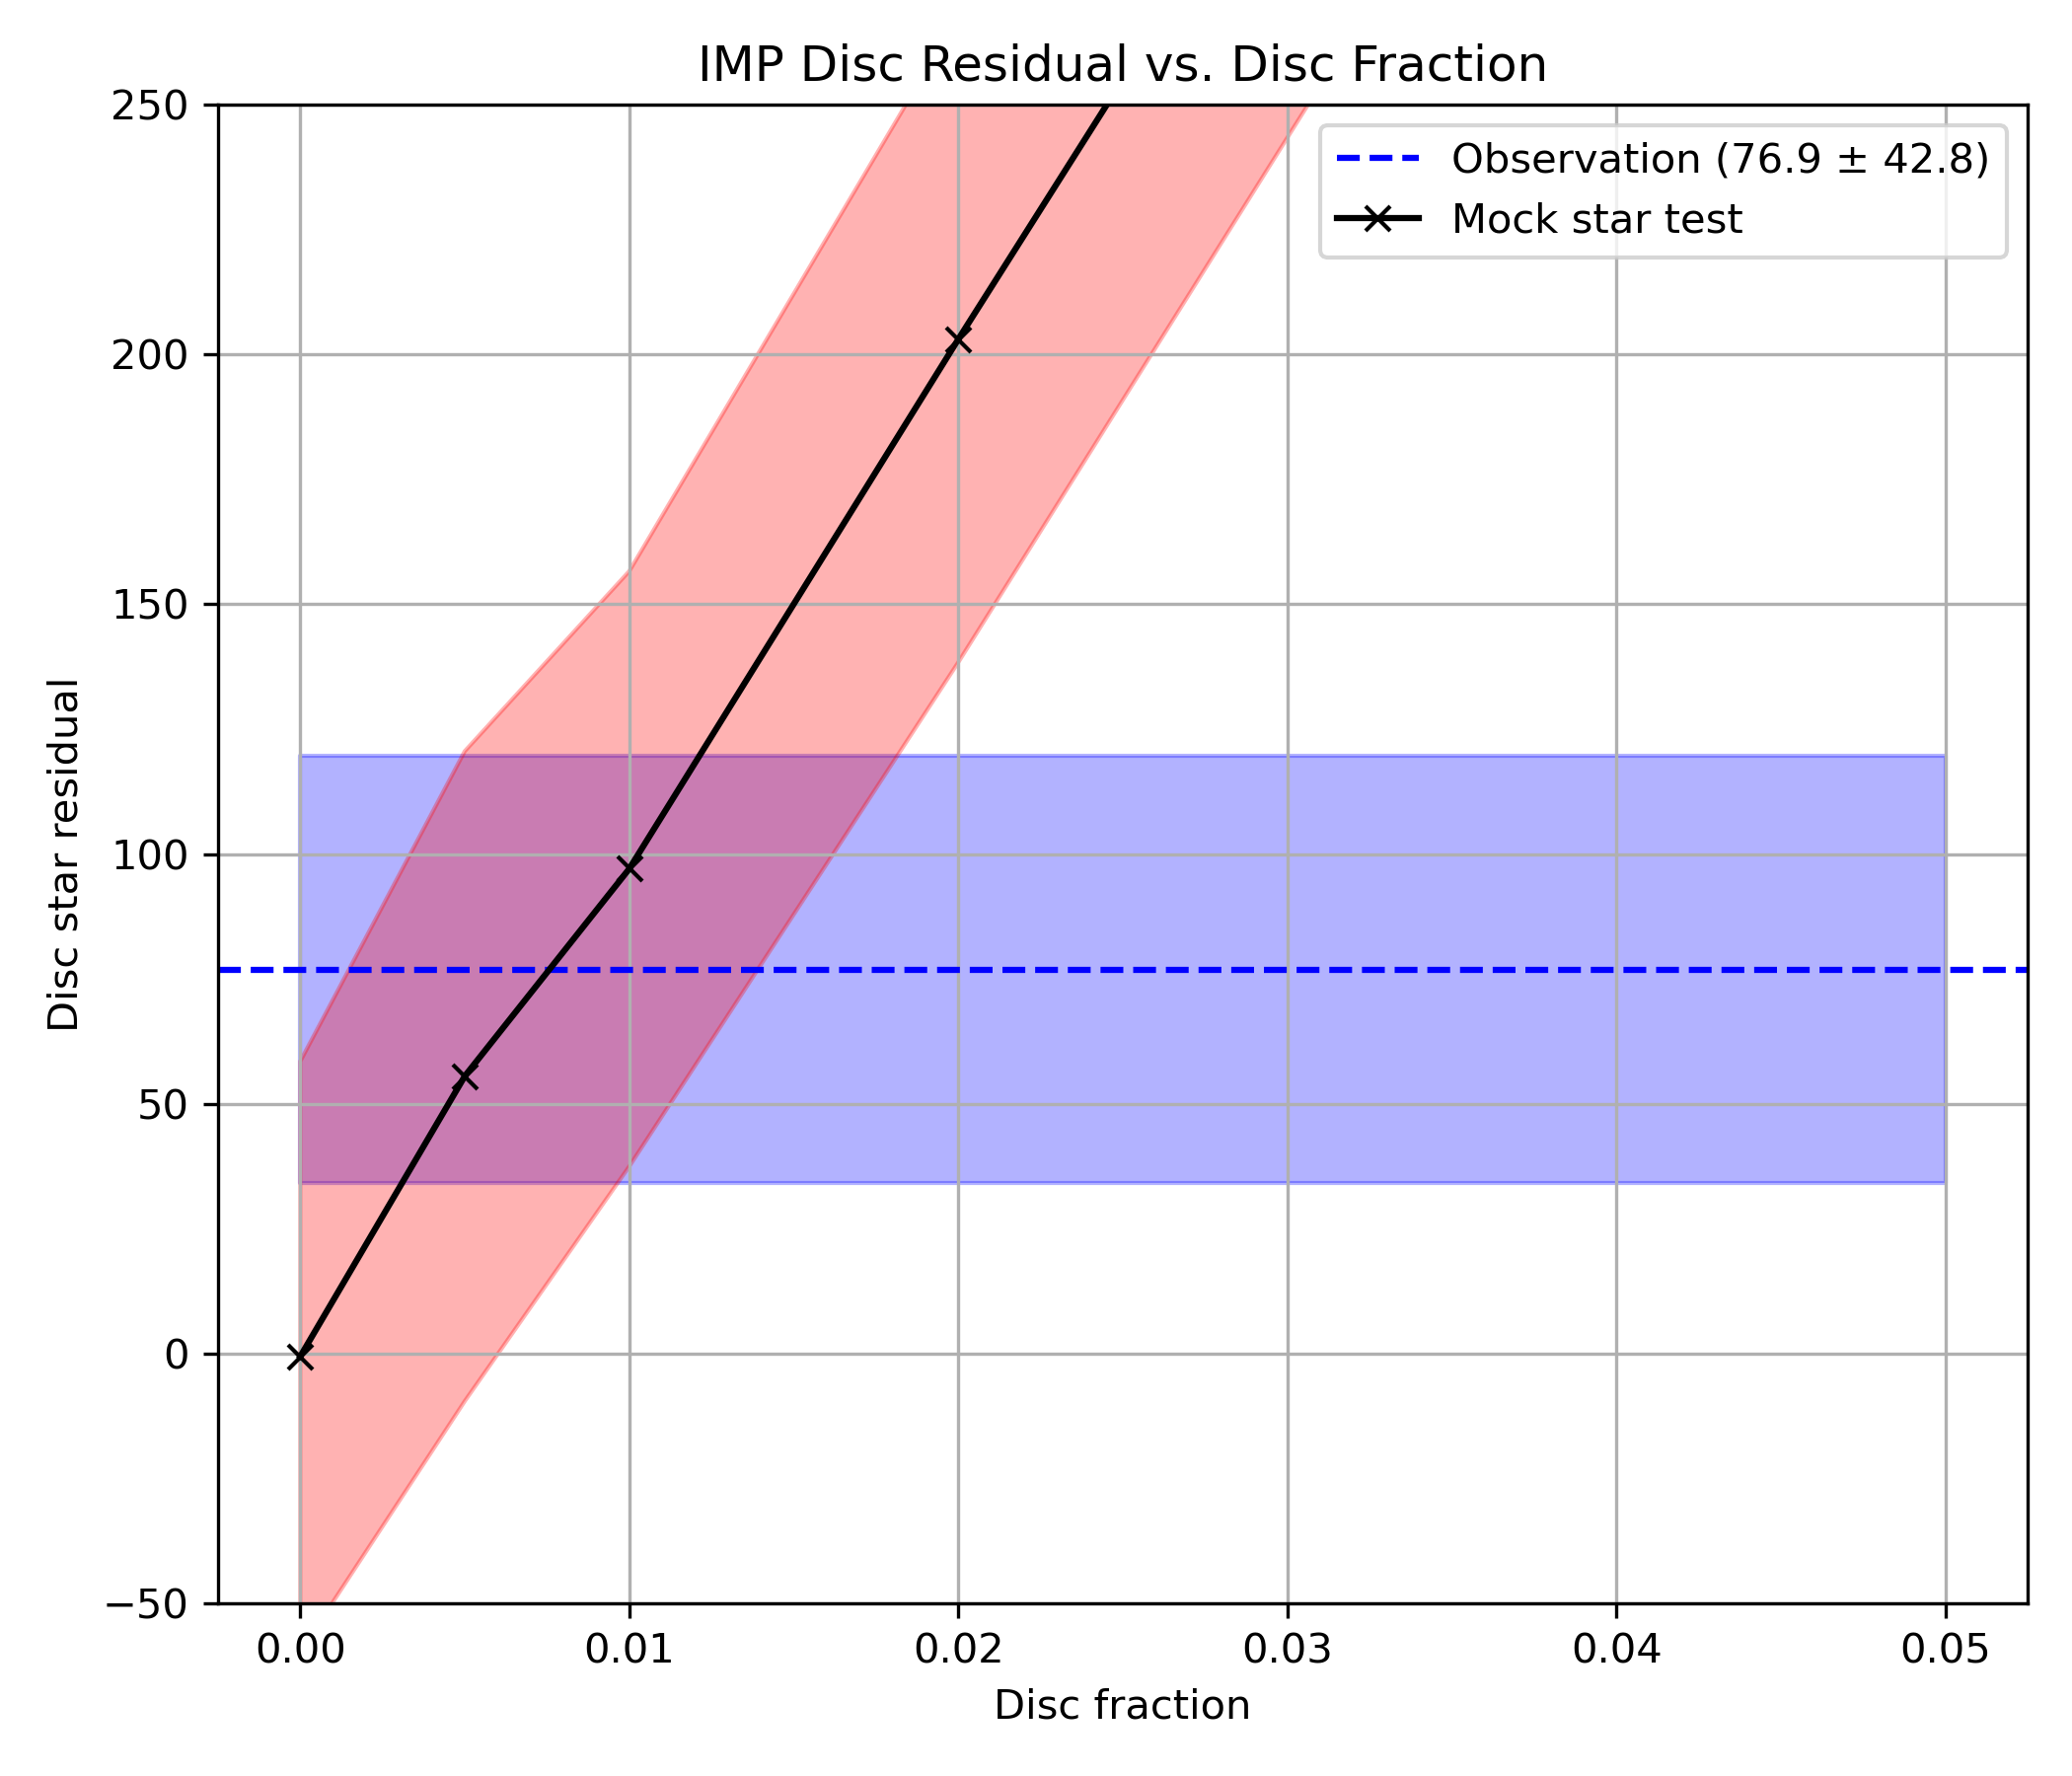
\includegraphics[width=0.49\textwidth]{../figures/imp_disc_fraction.png}
    \caption{Top: Normalised residual maps between observed and GMM-predicted 
    velocity distributions in $(v_R, v_\phi)$ for the VMP (left) and IMP (right) metallicity bins. 
    Grey ellipses show the $2\sigma$ contour of the fiducial thick disc model. Bottom: Disc residuals 
    as a function of injected disc fraction. The dashed line and blue band indicate the observed residual
     and its uncertainty. The solid black line and red region show mock test results and their uncertainties.
     (A reproduction of Figure 7 from \citet{zhang2024existencemetalpoordiscmilky})}
    \label{fig:residuals}
\end{figure}


\section{Extension Analysis}

We extend the work of \citet{zhang2024existencemetalpoordiscmilky} by adding the $\alpha$–element abundance, $[\alpha/\mathrm{Fe}]$, as a fourth dimension in our XD–GMM fits.  Following \citet{Vis2024}, each metallicity bin is split into “high–$\alpha$” and “low–$\alpha$” subsets (using XP abundances from \citealt{Li2024}), and the GMM is refit independently for each subset.  This chemo–kinematic dissection allows us to test whether the kinematic substructures in the very–metal–poor regime vary with $\alpha$–element enrichment, potentially distinguishing in situ from accreted populations.

\subsection{Alpha–Element Abundance}
\label{subsec:alpha}

The ratio $[\alpha/\mathrm{Fe}]$ traces the relative contributions of two supernova types: 
core–collapse (Type II) and thermonuclear (Type Ia). Type II supernovae result from the deaths of massive 
stars ($\gtrsim8\,M_\odot$) and explode on short timescales ($\sim10$–$30\,\mathrm{Myr}$) after star 
formation. They produce large amounts of $\alpha$-elements (O, Ne, Mg, Si, S, Ca, Ti), which are rapidly 
injected into the interstellar medium. In contrast, Type Ia supernovae arise from white dwarfs in binary 
systems, requiring hundreds of millions to billions of years to explode ($\gtrsim0.1$–$1\,\mathrm{Gyr}$). 
These events primarily enrich the interstellar medium with iron and iron-peak elements (e.g.\ Fe, Ni, Co).

Because the two channels operate on different timescales, the $[\alpha/\mathrm{Fe}]$ ratio encodes a 
population’s formation history:

\begin{itemize}
  \item \textbf{High–$[\alpha/\mathrm{Fe}]$:}  
    Rapid, intense star formation enriches the gas with $\alpha$-elements before Type Ia supernovae 
    contribute significant iron, leading to elevated $[\alpha/\mathrm{Fe}]$. These stars typically belong 
    to the in-situ thick disc, stellar halo, and ancient accreted debris. At fixed $[\mathrm{M/H}]$, 
    accreted populations (e.g.\ dwarf galaxies) generally show lower $[\alpha/\mathrm{Fe}]$ than in-situ 
    stars \citep{Helmi2018}, reflecting slower chemical evolution.
    
  \item \textbf{Low–$[\alpha/\mathrm{Fe}]$:}  
    A more extended star-formation history allows iron from Type Ia supernovae to accumulate, diluting 
    the $\alpha$ enrichment. This regime includes the thin disc, metal-rich bulge, and remnants of dwarf 
    satellites.
\end{itemize}

Hence, in the $[\alpha/\mathrm{Fe}]\!-\![\mathrm{M/H}]$ plane, populations that overlap in metallicity but 
formed on different timescales separate cleanly in $\alpha$ enrichment. By fitting separate XD–GMMs to the 
high– and low–$\alpha$ sequences within each metallicity bin, we can isolate how disc-like rotation and 
halo substructures depend on chemical evolution history.




\subsection{Data}
\label{subsec:data_vis}


We obtain the $\alpha$-to-metal abundance ratios from the
XP–based catalogue of \citet{Li2024}.
Following \citet{Vis2024}, we cross-match the XP-based $\alpha$ catalogue 
of \citet{Li2024} with the metallicity-selected red-giant branch sample . This base sample already 
incorporates the red-giant selection and photometric quality cuts from 
\citet{Andrae2023}, including limits on surface gravity, colour–magnitude 
position, and XP calibration reliability. 

To further ensure robust $\alpha$ abundances and kinematics, we apply 
several additional cuts:
\begin{itemize}\setlength\itemsep{2pt}
  \item we reject stars within $1^\circ$ of known dwarf galaxies and 
        those associated with globular clusters;
  \item a reddening cut $E(B-V)<0.5$ removes stars in regions of high 
        extinction, where XP abundances are less reliable;
  \item a Galactic latitude cut $|b|>10^\circ$ similarly avoids 
        the dust-dominated plane;
  \item we relax the fractional parallax uncertainty cut relative to 
        Section~\ref{subsec:datasample}, requiring only $\mathrm{fpu}<0.2$
        to retain sufficient stars in the metal-poor regime, which is 
        the focus of this analysis.
\end{itemize}


We obtain approximately 3.4 million stars in our final sample with alpha-element abundances.

Figure~\ref{fig:alphametal} shows the logarithmic density of our
RGB sample in the $[\alpha/\mathrm{M}]$–$[\mathrm{M/H}]$ plane.
Following \citet{Chandra_2024}, but with a deliberately tighter boundary as in \citet{Vis2024}:

\[
\begin{aligned}
\text{high-}\alpha:\;&
  \begin{cases}
    [\mathrm{M/H}] < -0.60 &
      [\alpha/\mathrm{M}] > 0.28 \\
    -0.60 \le [\mathrm{M/H}] \le 0.125 &
      [\alpha/\mathrm{M}] > -0.25[\mathrm{M/H}] + 0.13 \\
    [\mathrm{M/H}] > 0.125 &
      [\alpha/\mathrm{M}] > 0.10
  \end{cases} \\[4pt]
\text{low-}\alpha:\;&
  \begin{cases}
    [\mathrm{M/H}] < -0.80 &
      [\alpha/\mathrm{M}] < 0.21 \\
    -0.80 \le [\mathrm{M/H}] \le 0.07 &
      [\alpha/\mathrm{M}] < -0.21[\mathrm{M/H}] + 0.04
  \end{cases}
\end{aligned}
\]

This high-$\alpha$ threshold is raised so that the
chemistry of the Gaia–Sausage/Enceladus debris
\citep{Belokurov2018,Helmi2018} does not leak into the
in-situ sequence; the exclusion band between the branches is widened to maximise purity
in both sub-samples \citep{Vis2024}.

\begin{figure}[H]
    \centering
    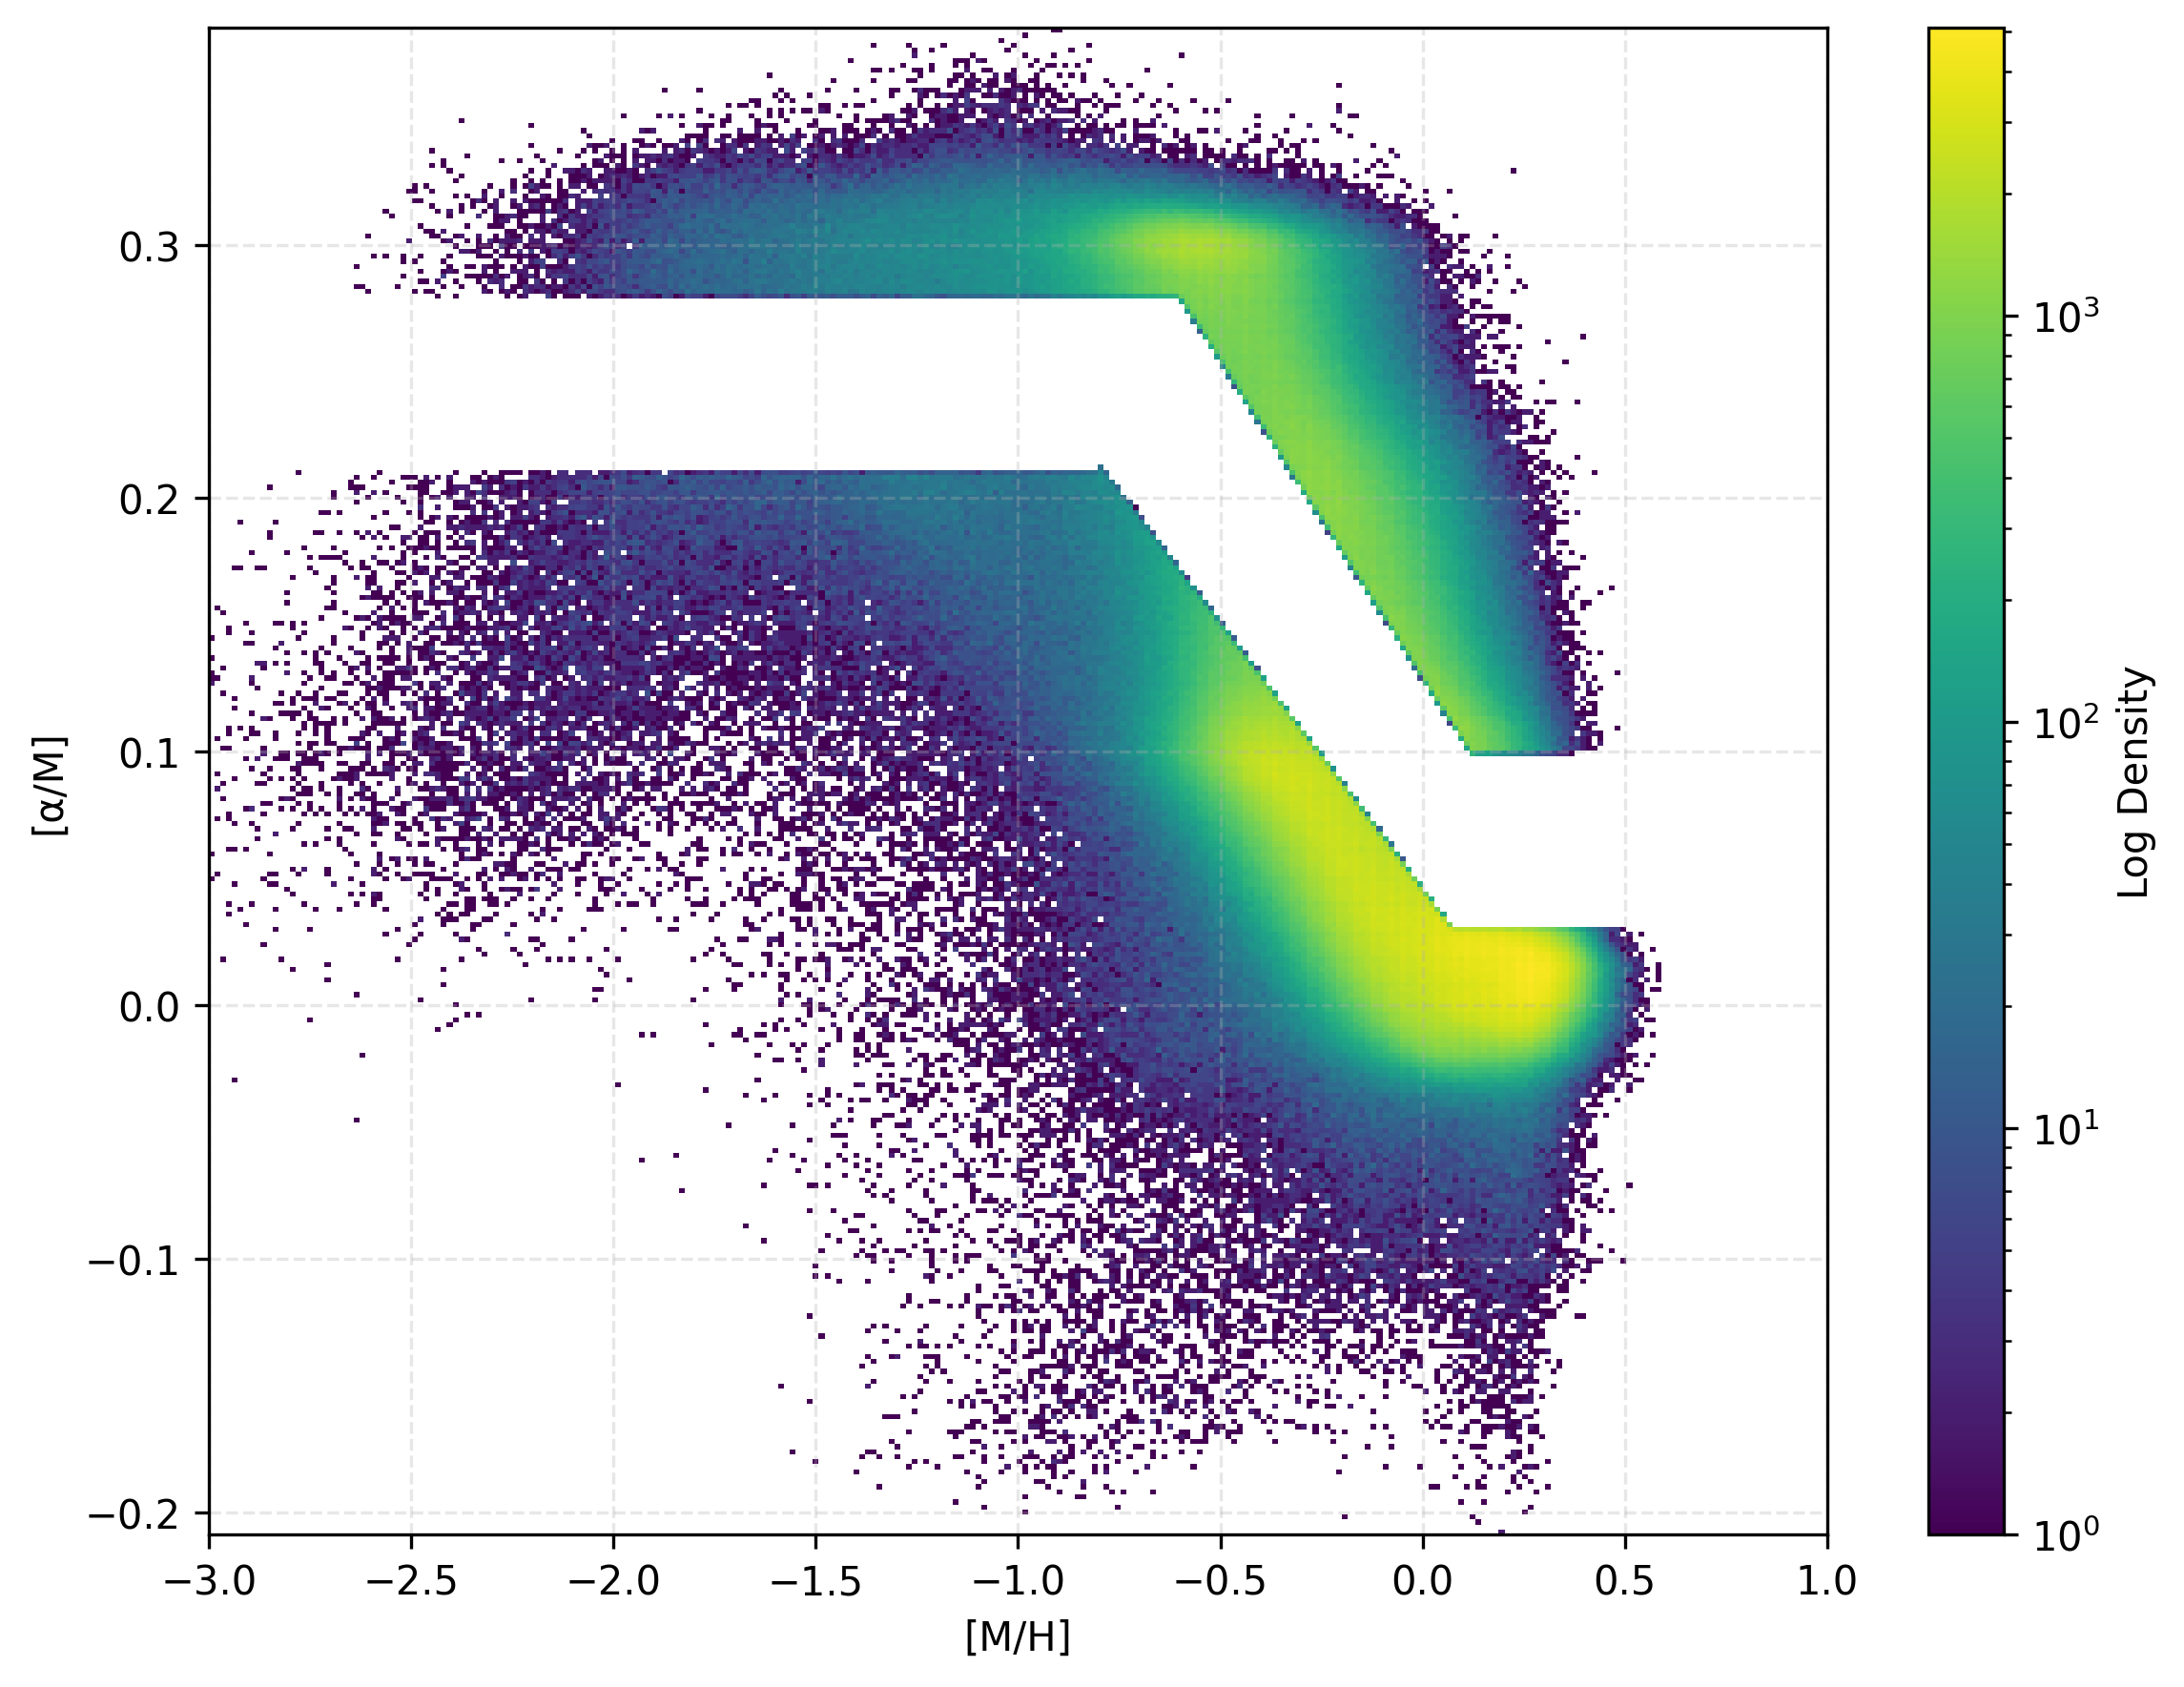
\includegraphics[width=0.49\textwidth]{../figures/alpha_vs_metalicity.png}
    \caption{Density of stars in the $[\alpha/\mathrm{M}]$–$[\mathrm{M/H}]$ plane.
             The high-$\alpha$ and low-$\alpha$ sequences are separated by the
             piecewise linear boundary described in the text. The transition zone
             between the two sequences is clearly removed from this plot and discarded from
             subsequent analysis. (A reproduction of Figure 1 in \citet{Vis2024})}
    \label{fig:alphametal}
\end{figure}


Figure~\ref{fig:rz_metallicity} shows the distribution of our sample in cylindrical Galactocentric radius 
$R$ versus height above the midplane $z$, colour–coded by the mean metallicity in each pixel. The top panel 
presents this distribution for the full RGB sample, while the bottom panels split the data into high–$\alpha$ 
(left) and low–$\alpha$ (right) subsamples. 

\begin{figure}[H]
  \centering
  \begin{subfigure}{0.6\textwidth}
    \centering
    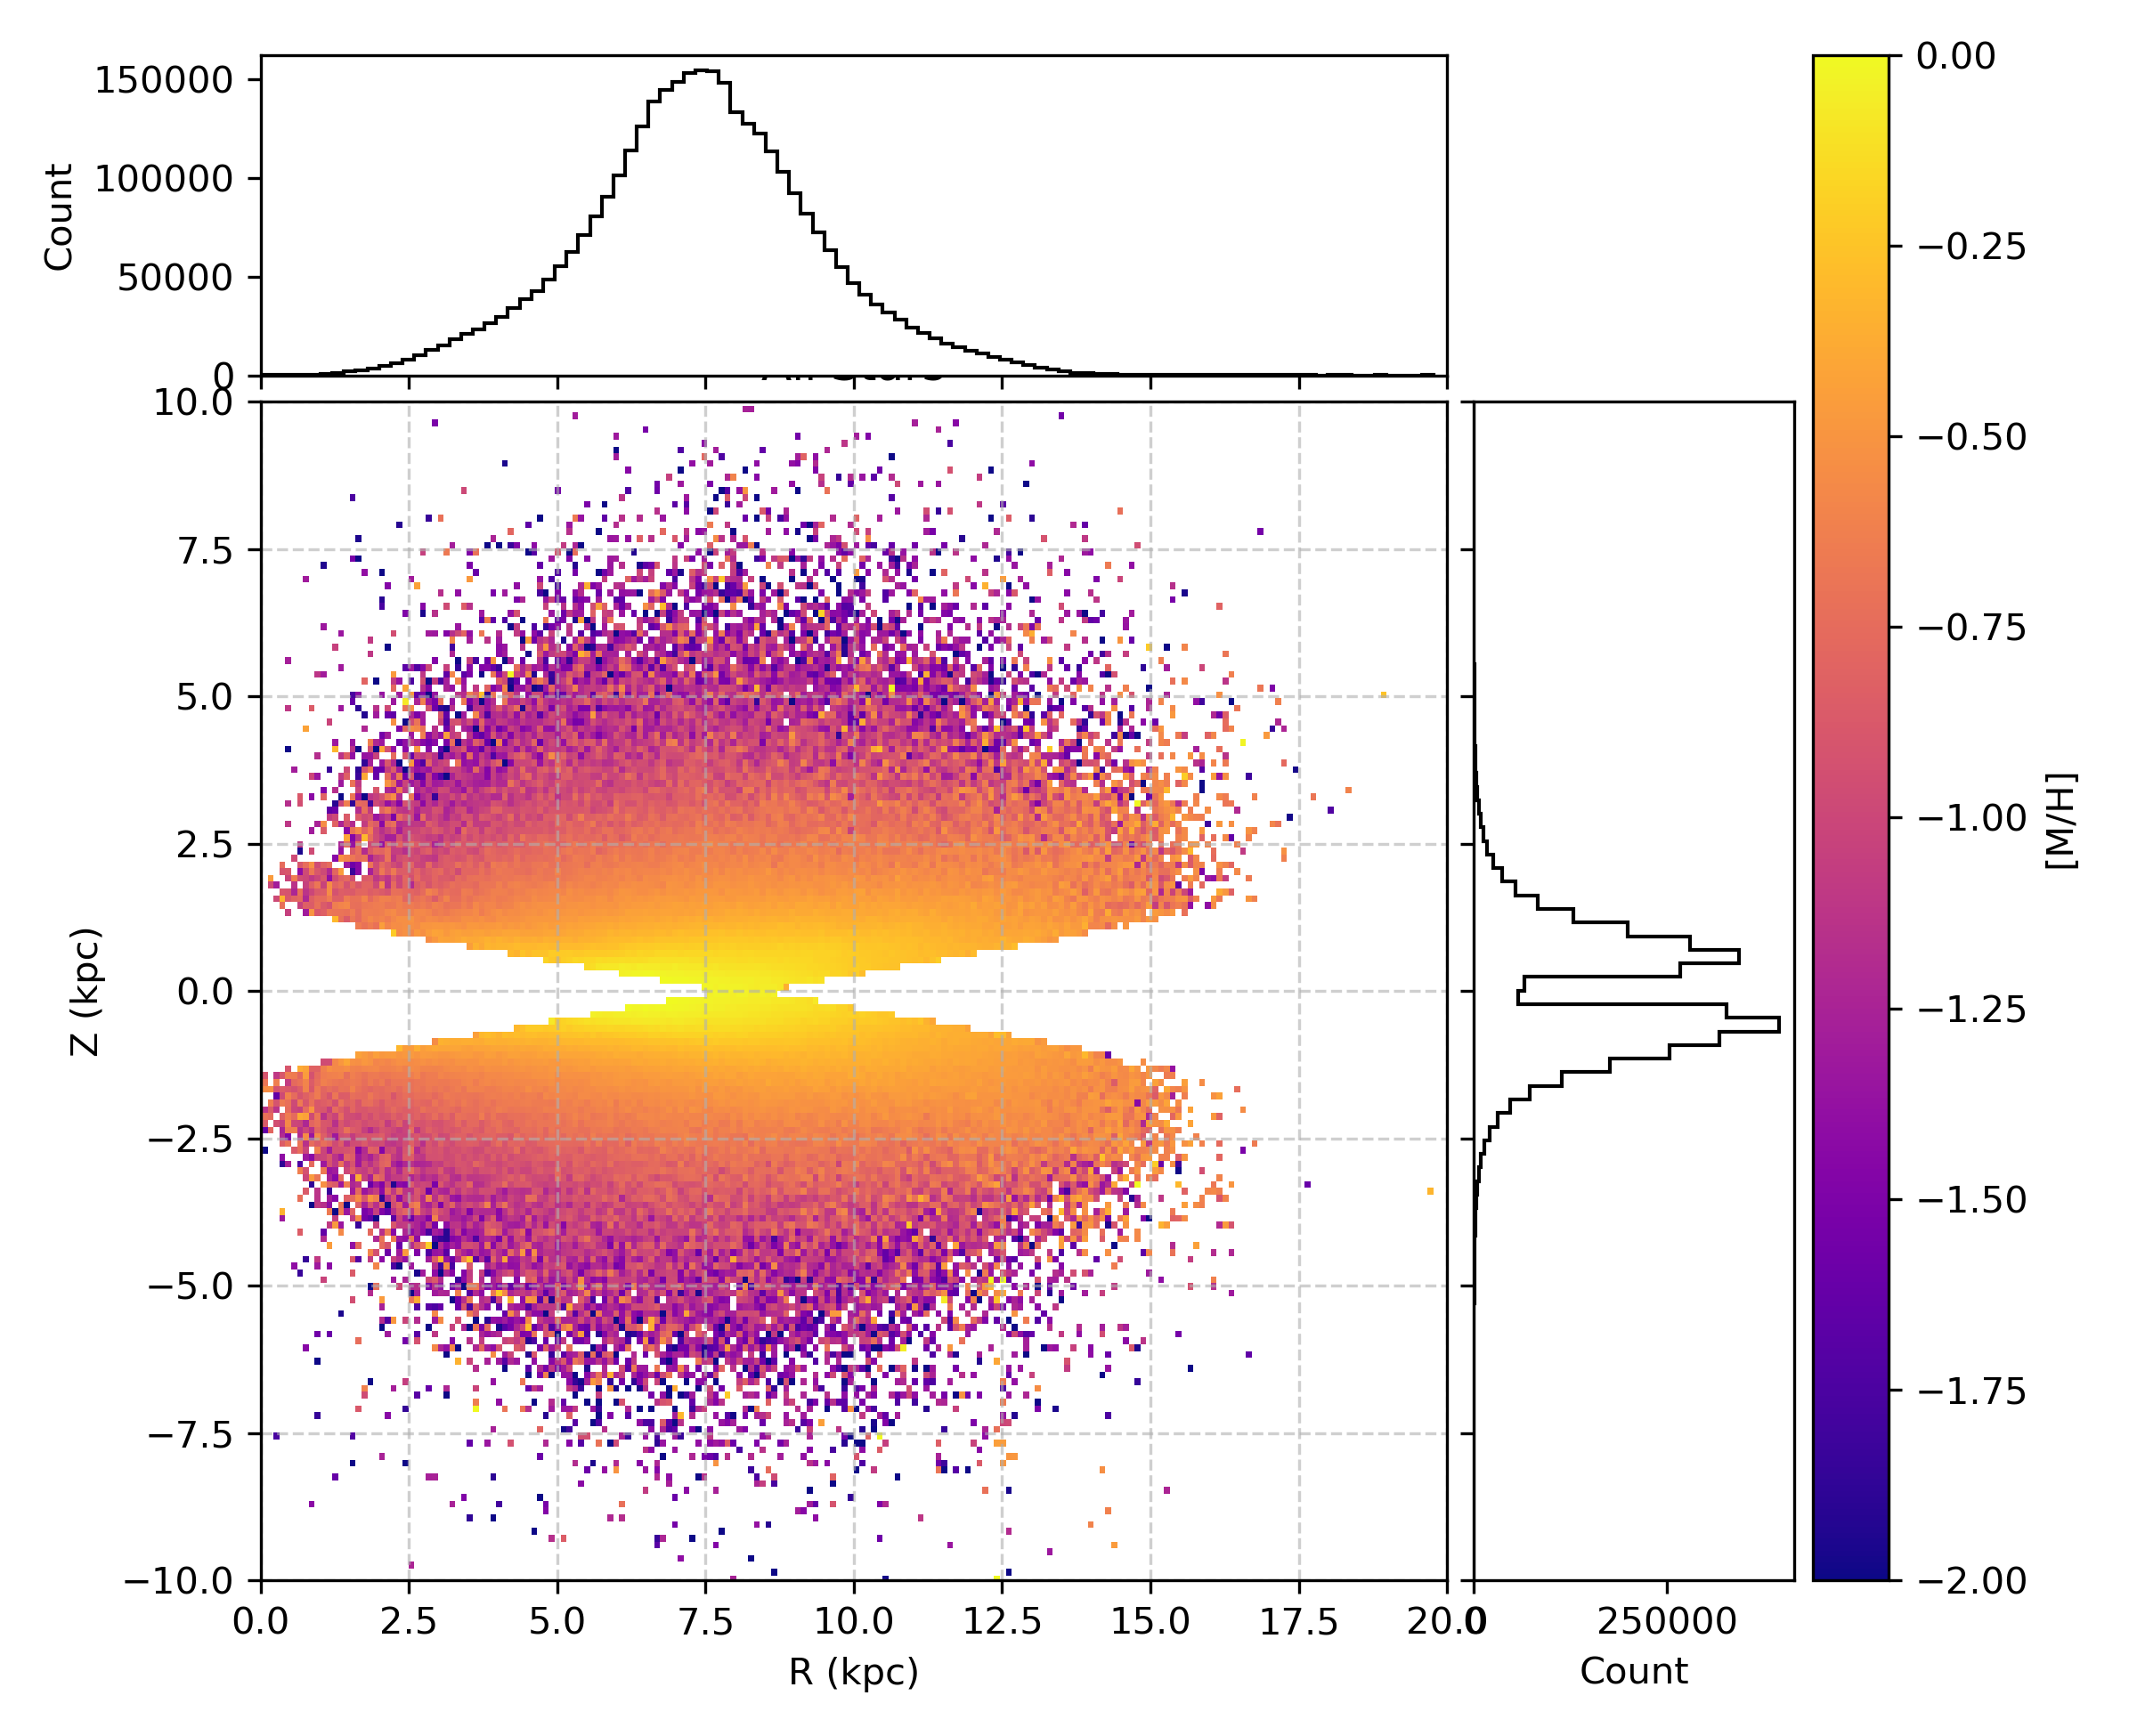
\includegraphics[width=\textwidth]{../figures/vis_rz_metallicity_all.png}
    \caption{All RGB stars}
    \label{fig:rz_all}
  \end{subfigure}

  \vspace{0.8em}

  \begin{subfigure}{0.45\textwidth}
    \centering
    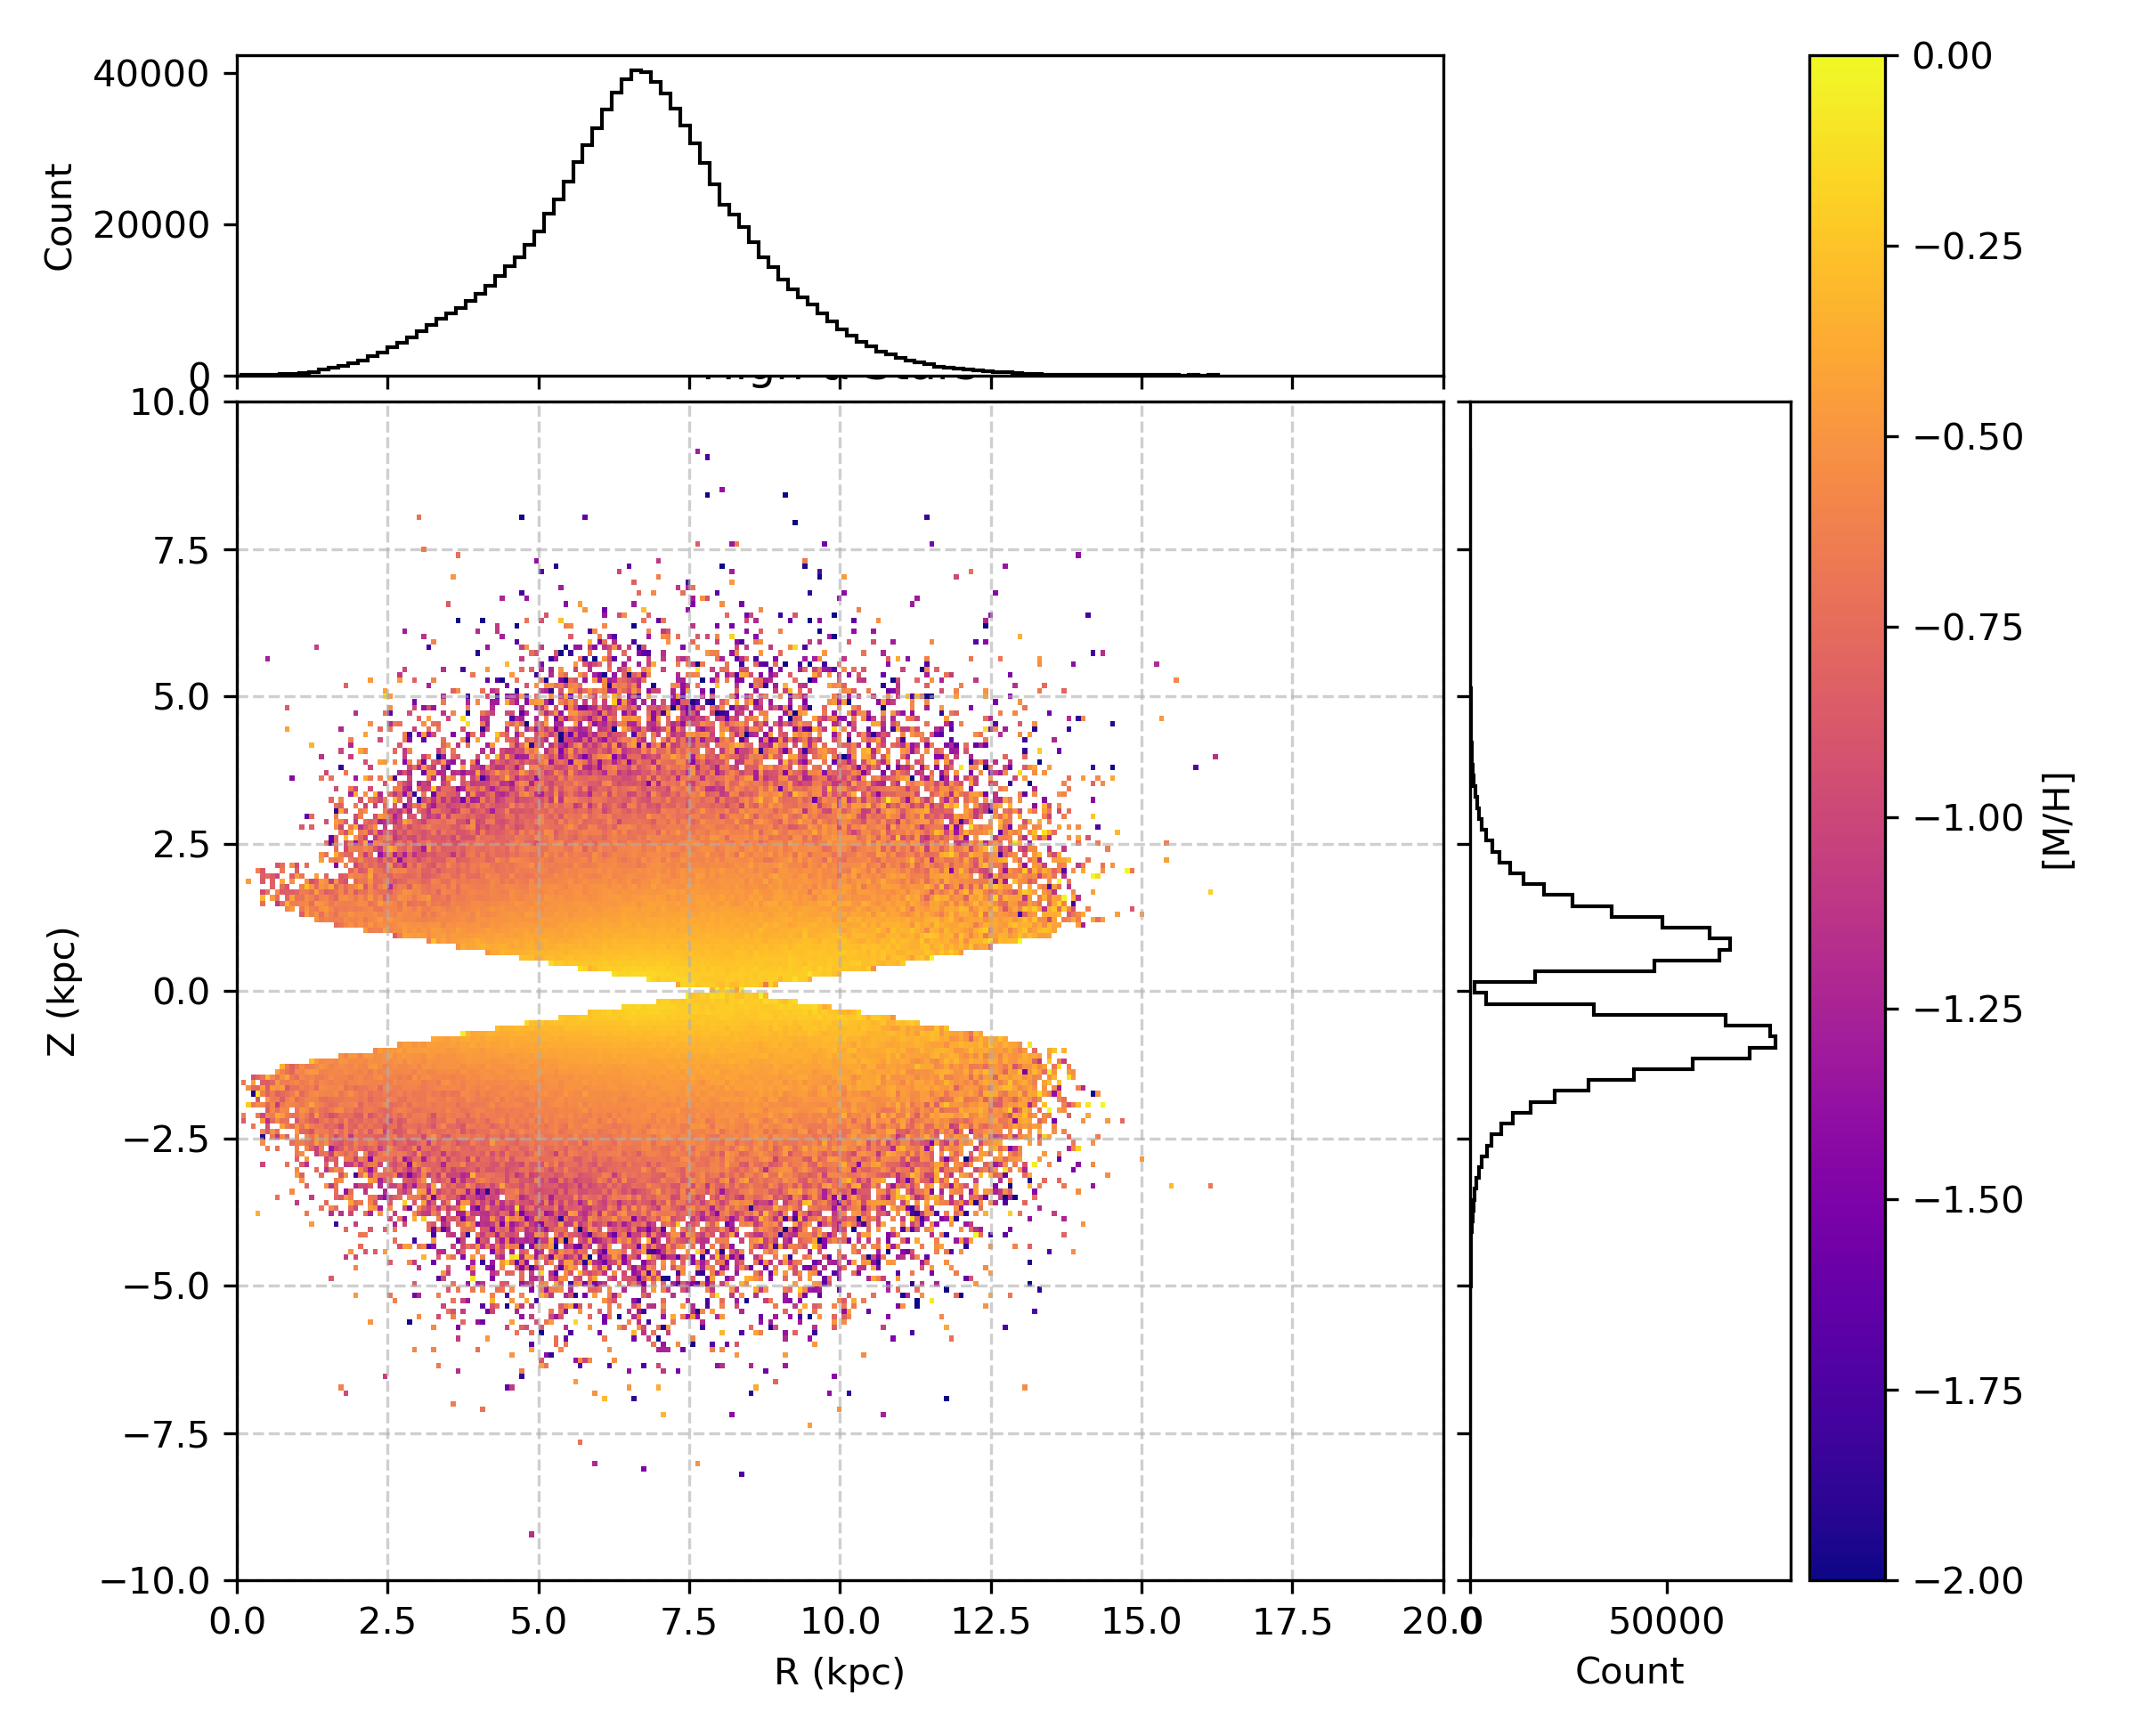
\includegraphics[width=\textwidth]{../figures/vis_rz_metallicity_high_alpha.png}
    \caption{High-$\alpha$ subsample}
    \label{fig:rz_highalpha}
  \end{subfigure}\hfill
  \begin{subfigure}{0.45\textwidth}
    \centering
    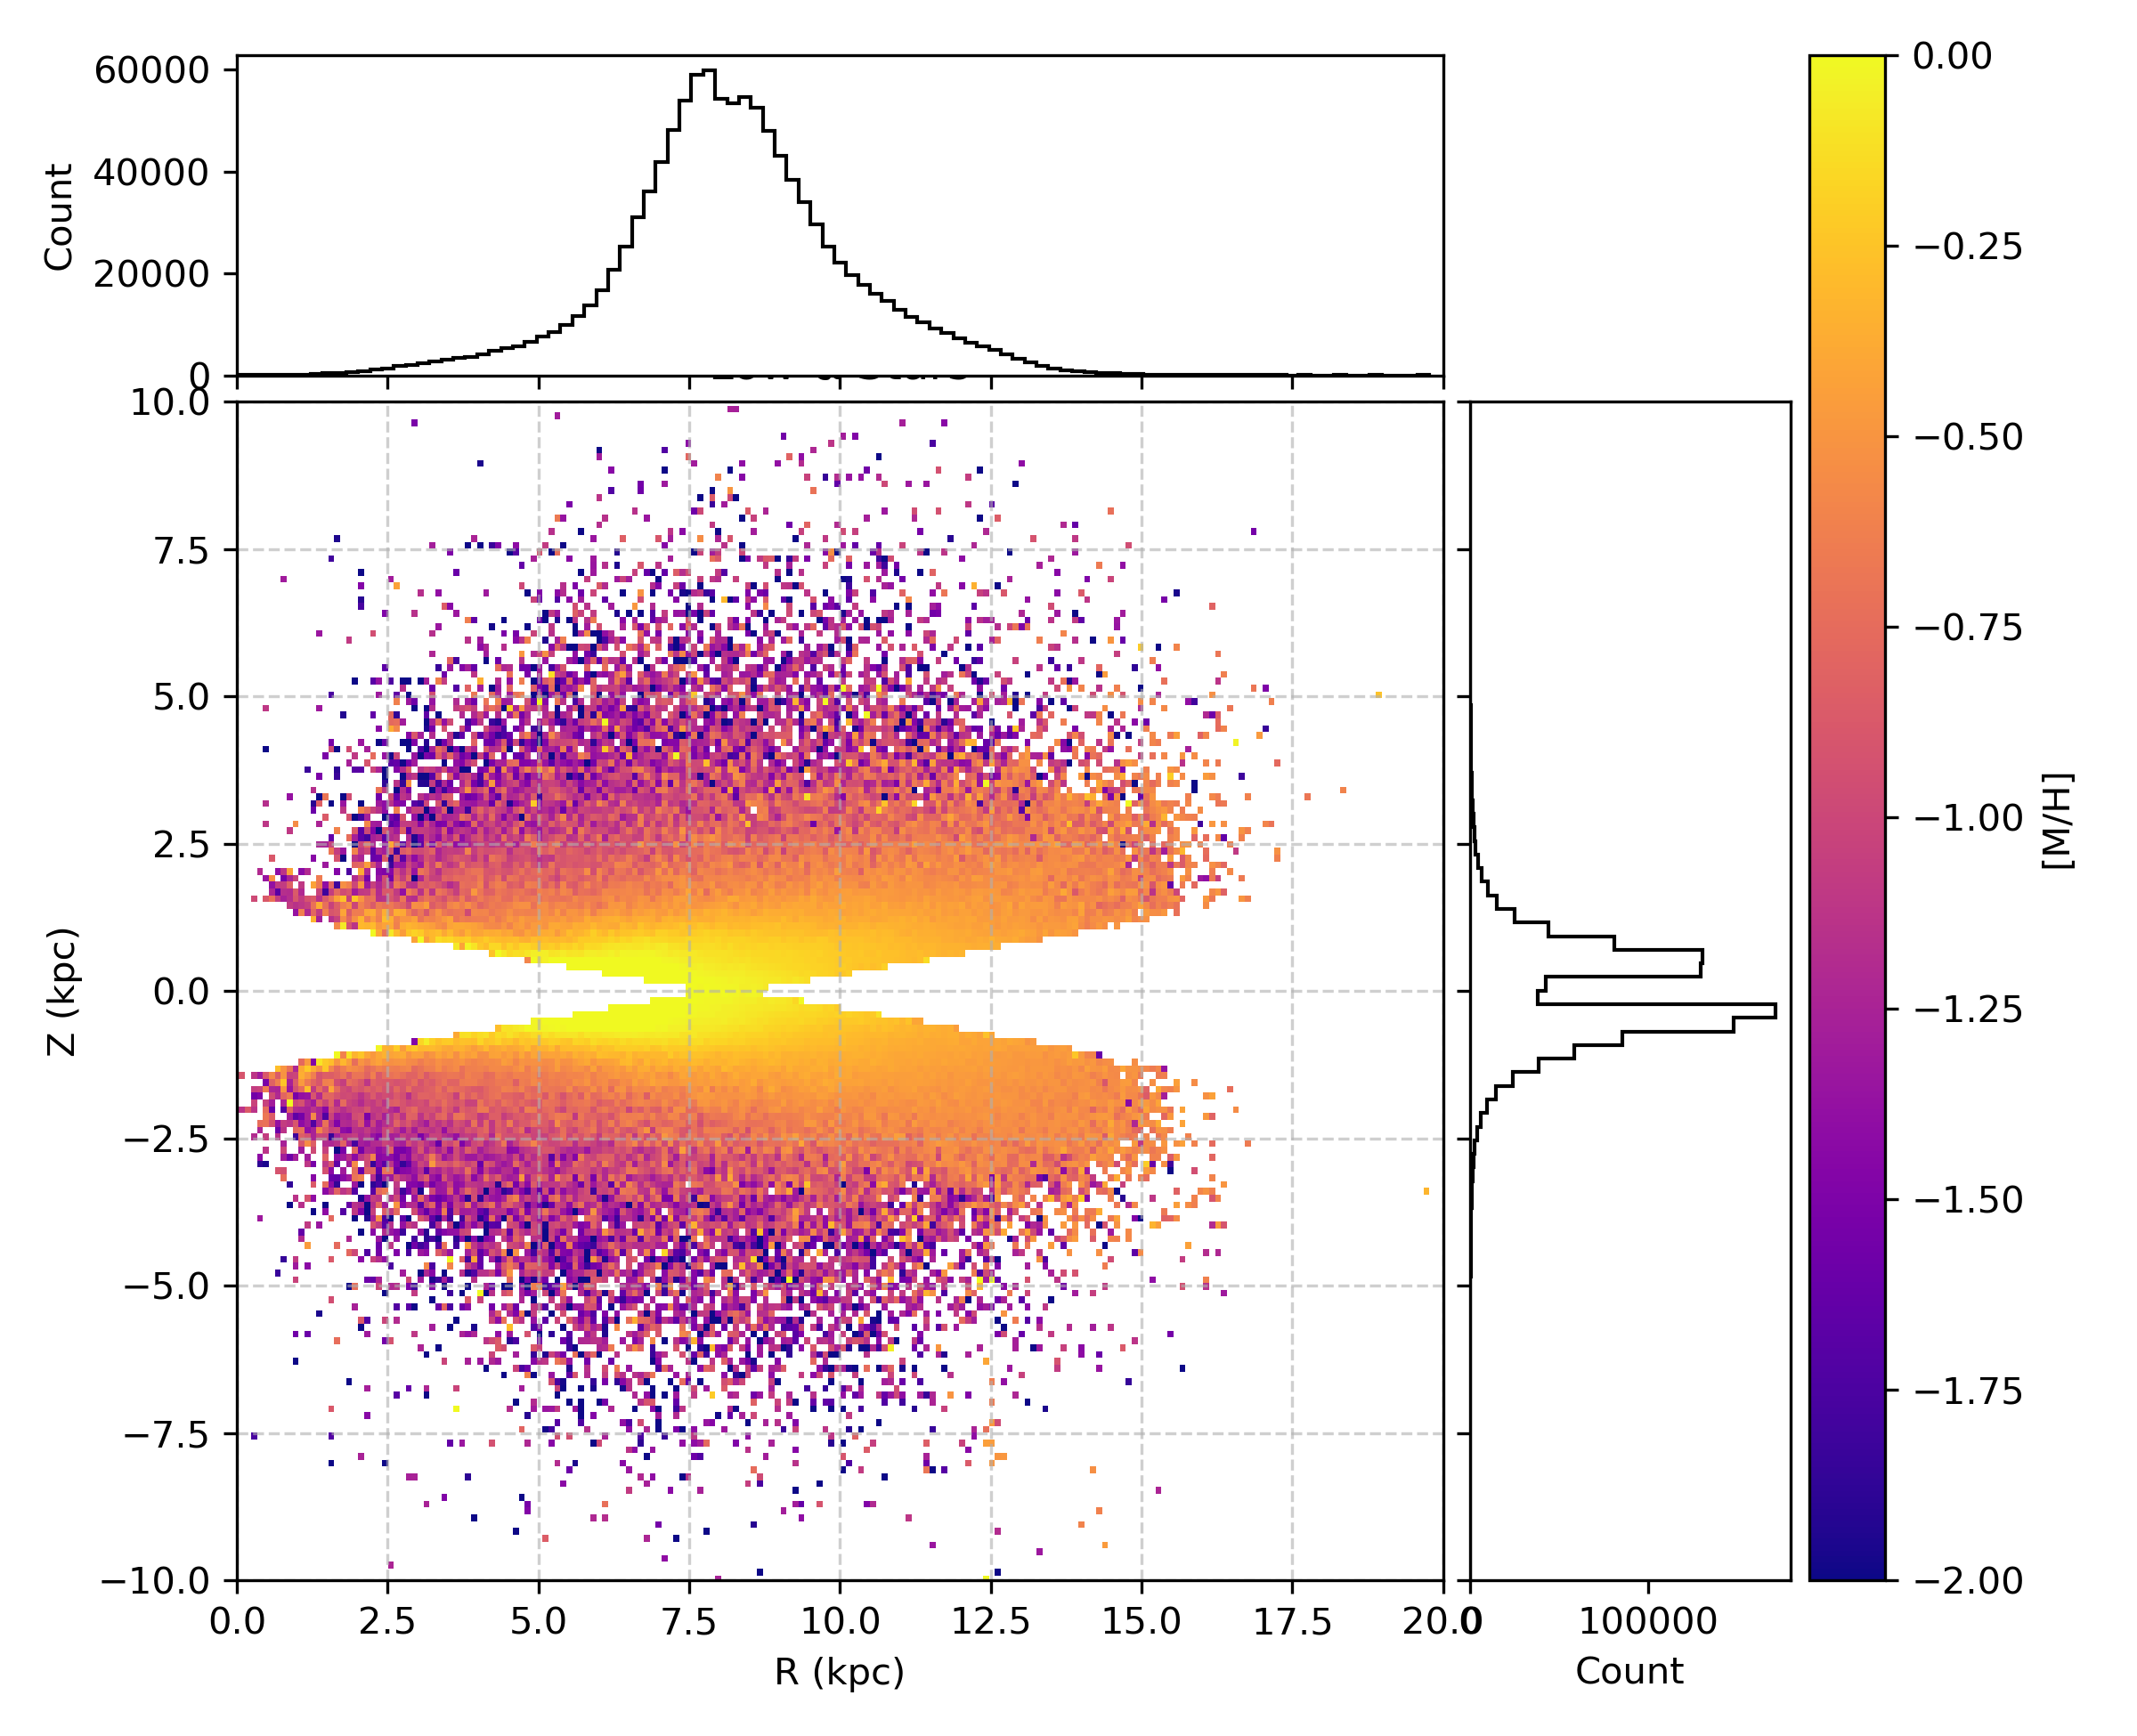
\includegraphics[width=\textwidth]{../figures/vis_rz_metallicity_low_alpha.png}
    \caption{Low-$\alpha$ subsample}
    \label{fig:rz_lowalpha}
  \end{subfigure}

  \caption{Mean $[\mathrm{M/H}]$ colour–coded in the
           Galactocentric $R$–$z$ plane.  
           \textit{Top:} the complete $G<16$ RGB sample.
           \textit{Bottom left:} high-$\alpha$ stars; \textit{bottom right:} low-$\alpha$ stars.
           The high-$\alpha$ population is more centrally concentrated and
           shows a shallower vertical metallicity gradient. (A reproduction of
           Figure 2 in \citet{Vis2024}) }
  \label{fig:rz_metallicity}
\end{figure}

The high–$\alpha$ population is more centrally concentrated and spans a smaller range in $R$ and $z$ than the 
low–$\alpha$ stars. The broader vertical extent of the low–$\alpha$ sequence likely reflects contributions 
from accreted material at large scale heights. A steep negative metallicity gradient with increasing $z$ is 
evident in the low–$\alpha$ sample and also visible in the full sample, likely due to the dominance of 
low–$\alpha$ stars in the overall dataset. In contrast, the high–$\alpha$ population exhibits a shallower 
vertical metallicity gradient and a thicker disc structure. We also observe a metallicity gradient towards 
larger $R$ in the low–$\alpha$ disc, indicative of radial migration and consistent with flaring commonly 
seen in the Galactic thin disc \citep[e.g.][]{Haywood2013,ratcliffe2023}.


To trace how rotational support evolves with metallicity and $\alpha$–element enrichment, following \citet{Vis2024} 
we examine the distribution of azimuthal velocity ($v_\phi$) as a function of $[\mathrm{M/H}]$.  
Figure~\ref{fig:mh_vphi_alpha} presents this relation for (i) the full RGB sample, and (ii) the chemically 
separated high–$\alpha$ and low–$\alpha$ subsamples derived in Section~\ref{subsec:alpha}.  Each panel shows 
the column-normalised density in the $[\mathrm{M/H}]$–$v_\phi$ plane together with running medians 
(red dashed) and 16th/84th percentiles (black).

\begin{figure}[H]
  \centering
  %--------------------------- full sample --------------------------
  \begin{subfigure}[b]{0.32\textwidth}
    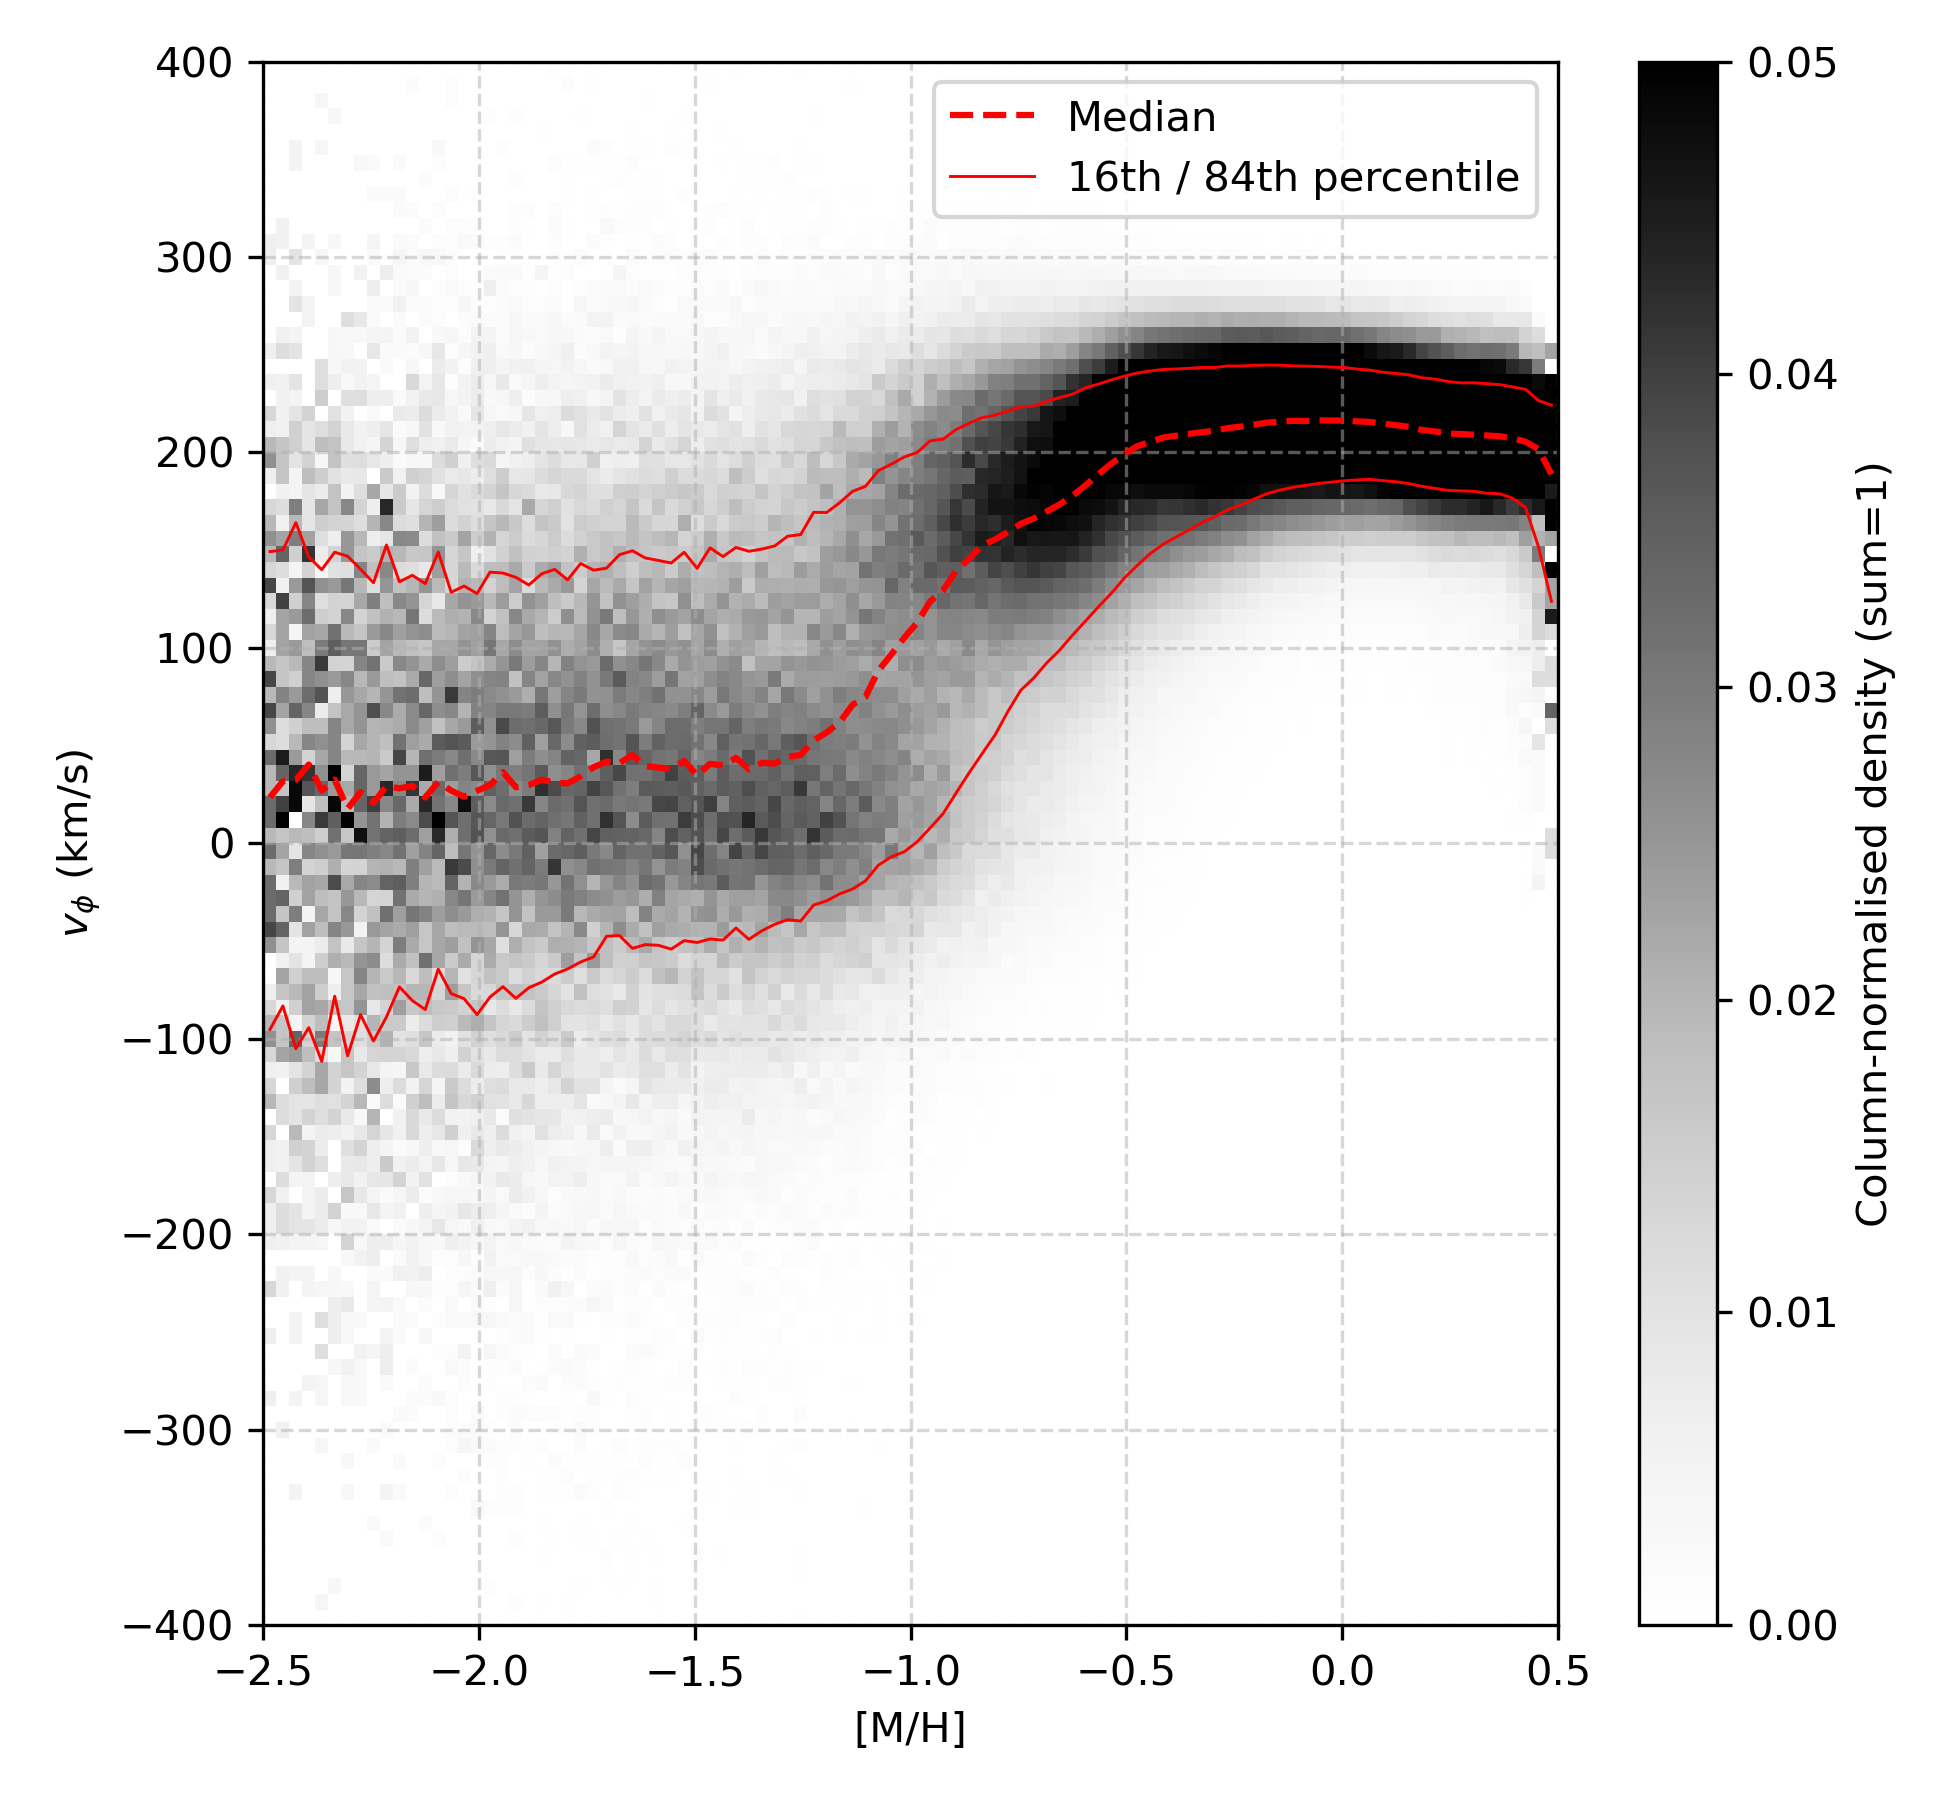
\includegraphics[width=\textwidth]{../figures/vis_mh_vphi_all.png}
    \caption{All RGB stars}
  \end{subfigure}\hfill
  %-------------------------- high-α sample --------------------------
  \begin{subfigure}[b]{0.32\textwidth}
    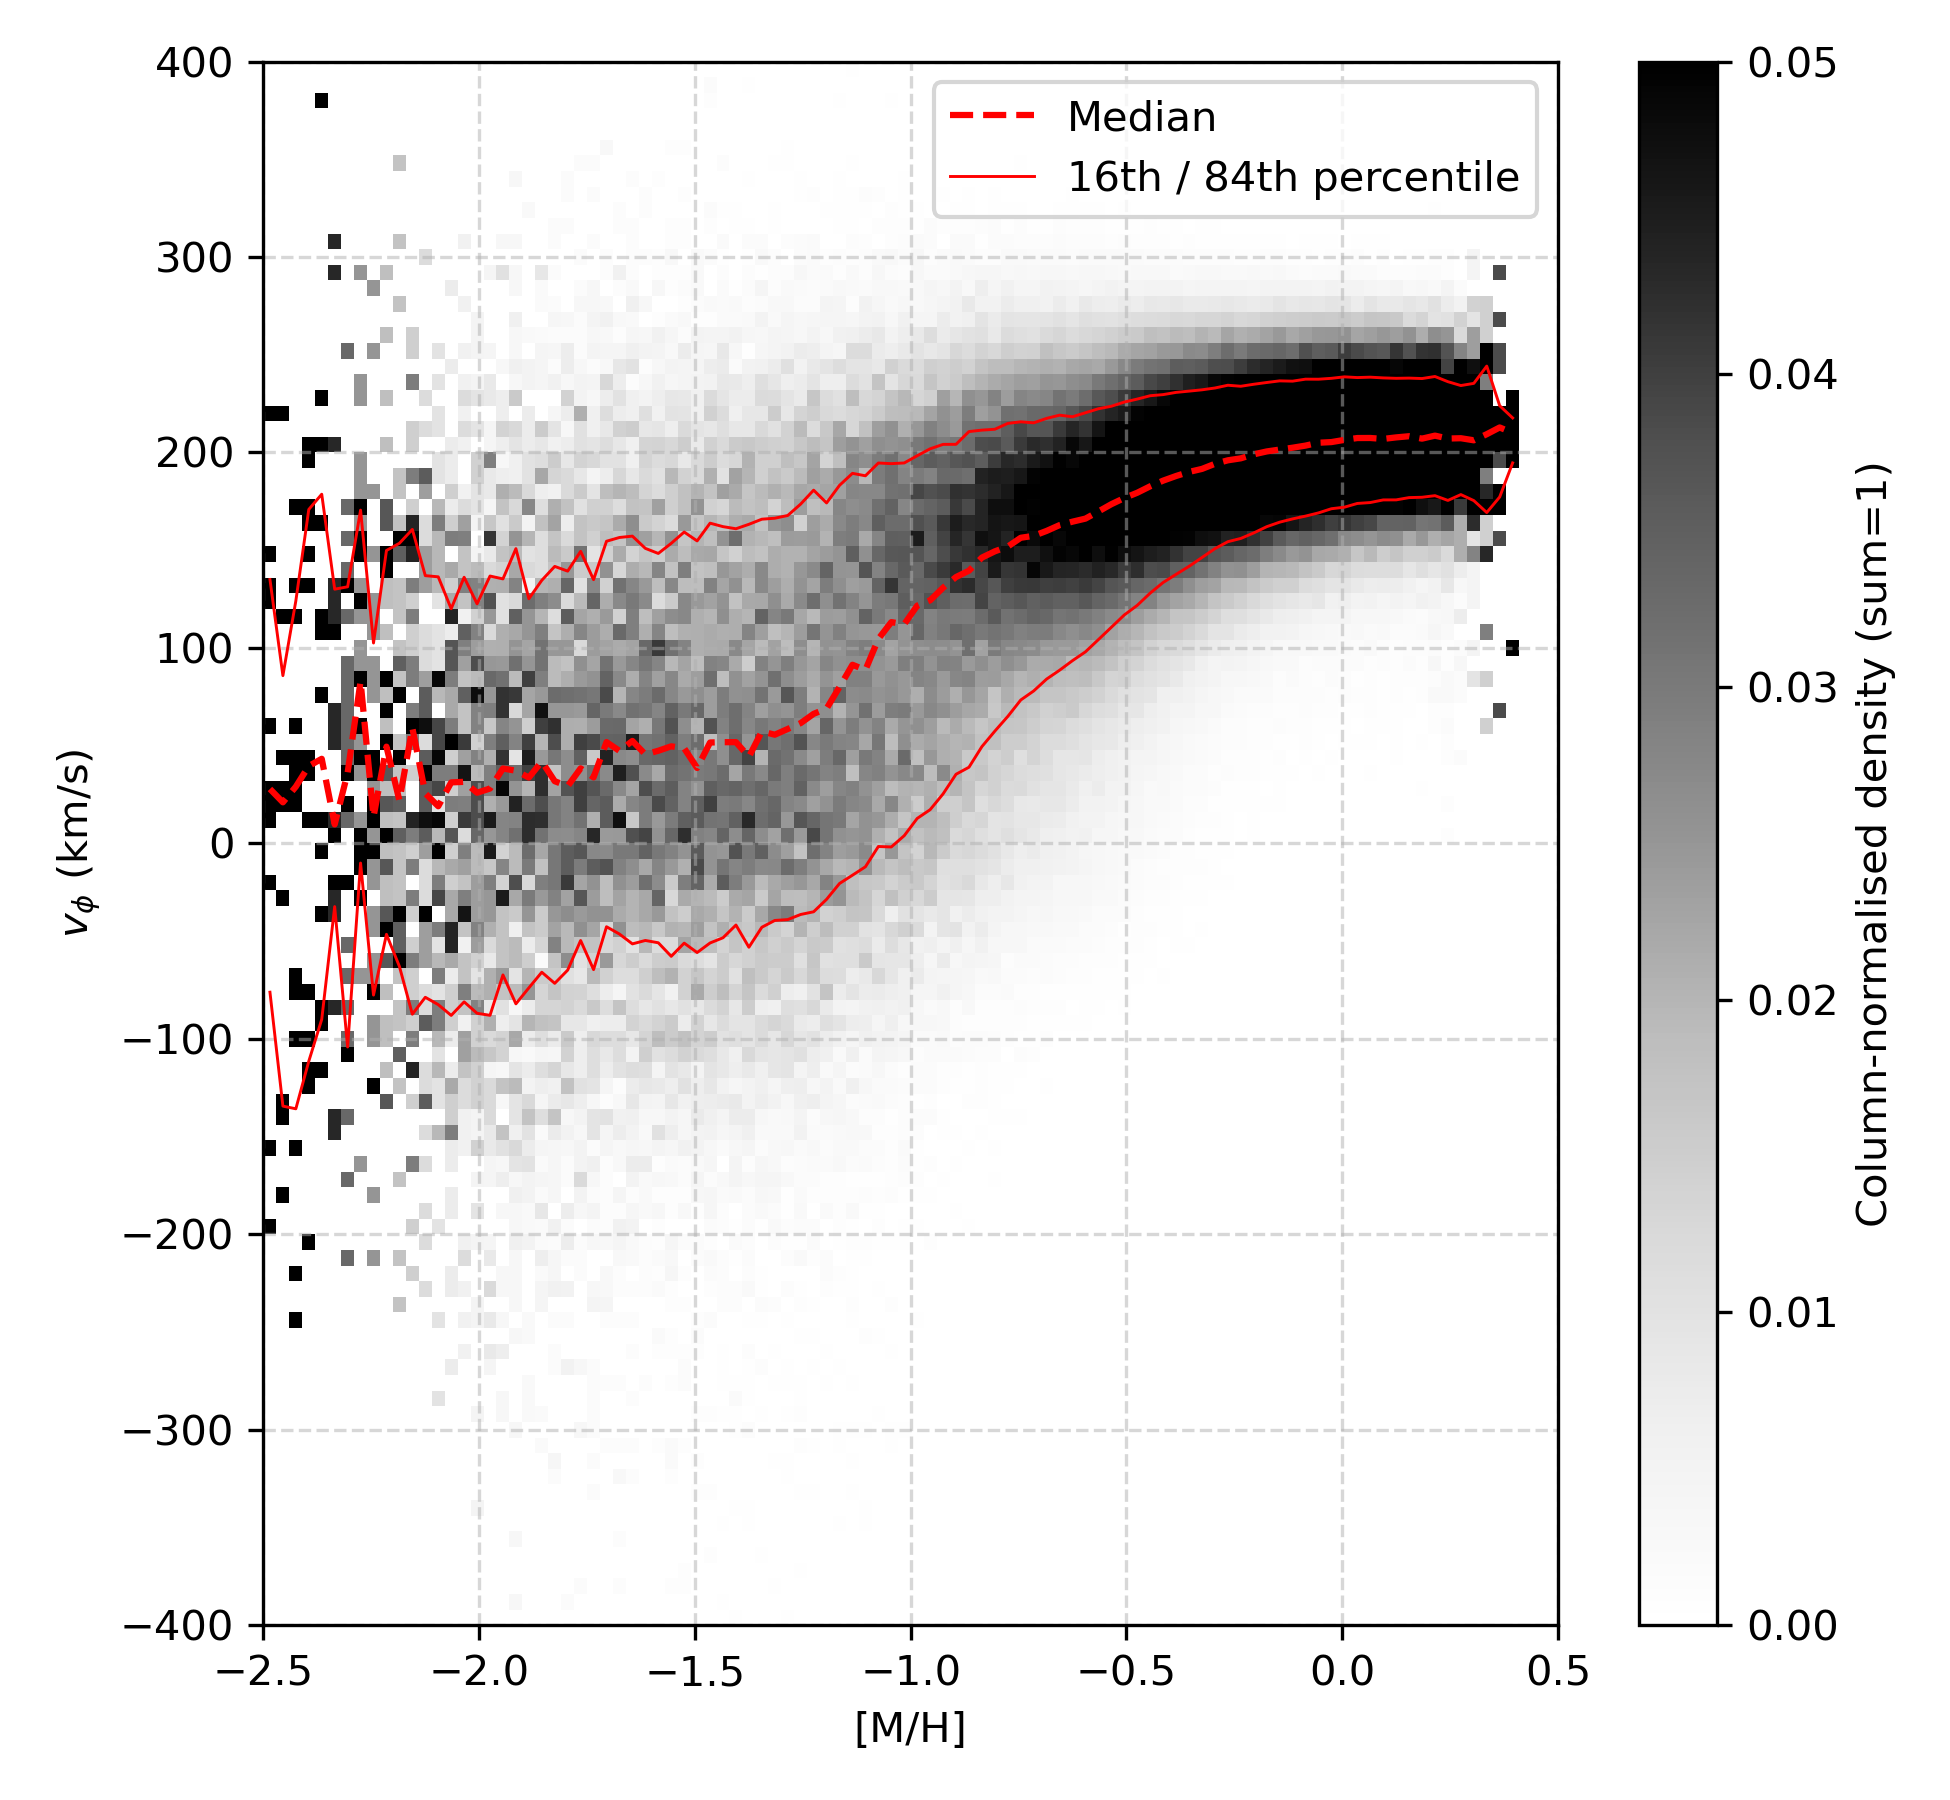
\includegraphics[width=\textwidth]{../figures/vis_mh_vphi_high_alpha.png}
    \caption{High-$\alpha$ sequence}
  \end{subfigure}\hfill
  %-------------------------- low-α sample ---------------------------
  \begin{subfigure}[b]{0.32\textwidth}
    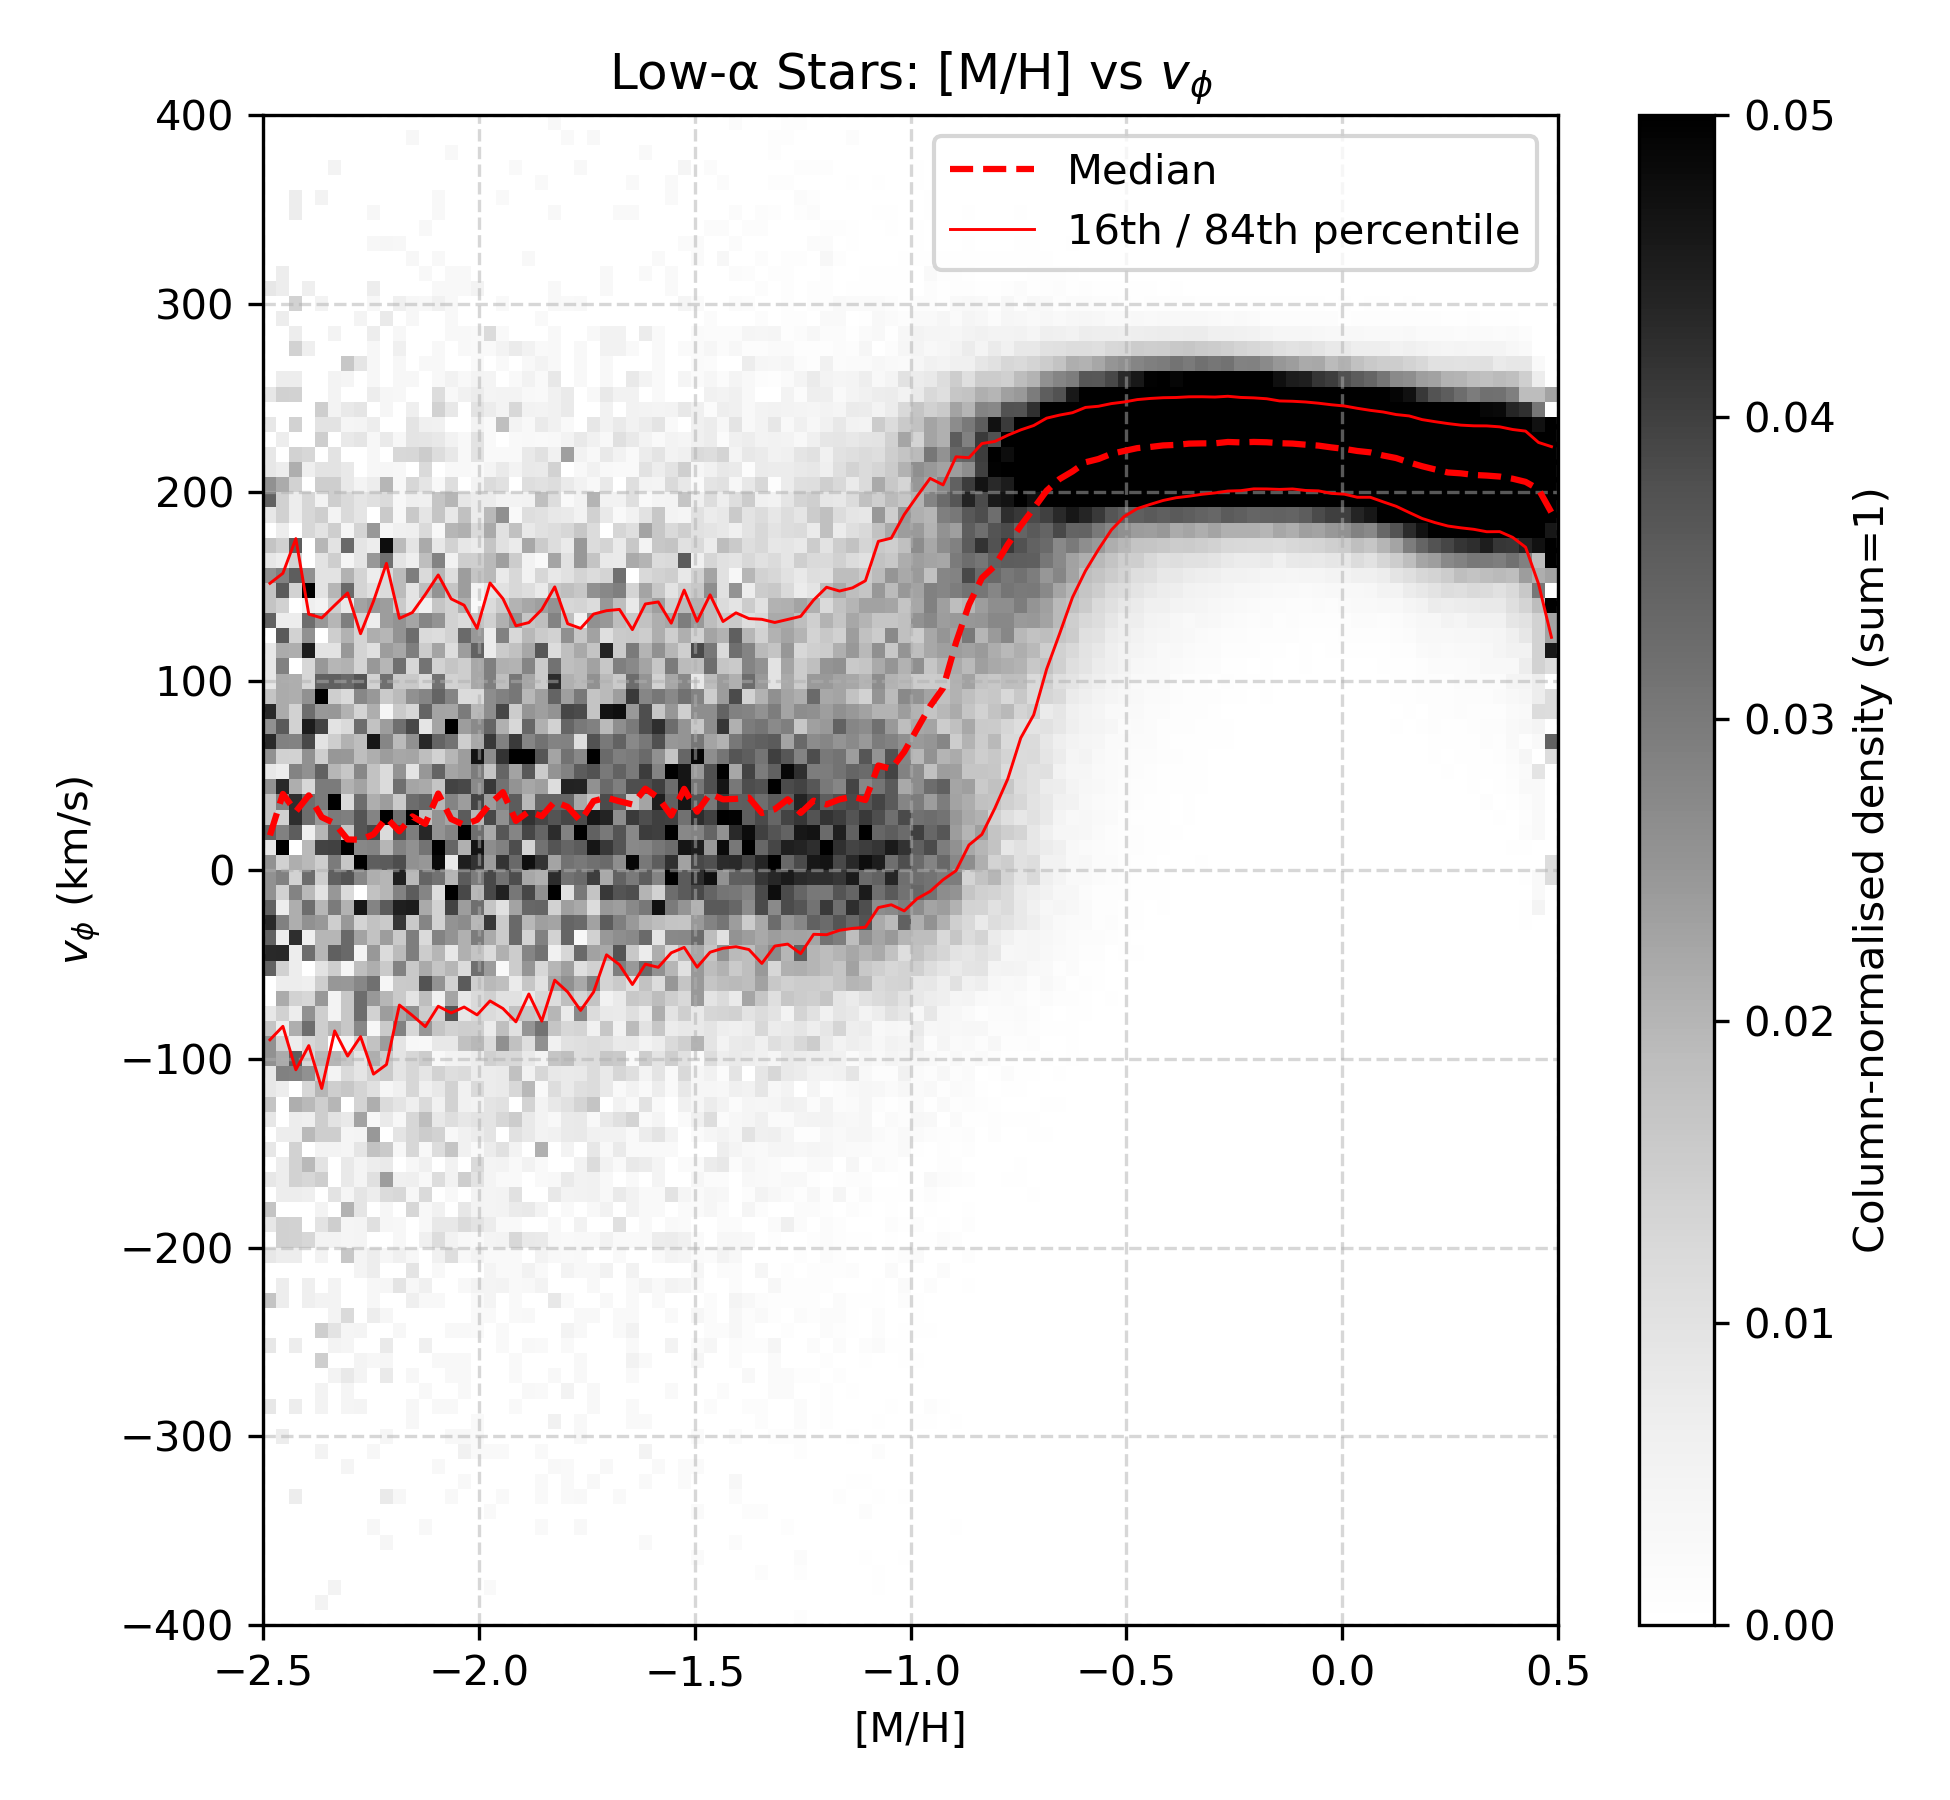
\includegraphics[width=\textwidth]{../figures/vis_mh_vphi_low_alpha.png}
    \caption{Low-$\alpha$ sequence}
  \end{subfigure}

  \caption{Azimuthal velocity versus metallicity.  
           Left: full RGB sample.  
           Centre: high-$\alpha$ stars.  
           Right: low-$\alpha$ stars.  
           Contours show running medians (red) and the 16th/84th percentiles (black).  
           (Adapted from Fig.\,3 of \citealt{Vis2024}.)}
  \label{fig:mh_vphi_alpha}
\end{figure}

The high-$\alpha$ giants 
exhibit a gradual spin-up with increasing metallicity.  
At low metallicities ($[\mathrm{M/H}]\lesssim -2$), the population 
shows mild net prograde rotation with large dispersion, 
consistent with a dynamically hot stellar halo. From $[\mathrm{M/H}]\gtrsim -1.3$, 
there is a steady increase in rotation velocity and a corresponding decrease in 
dispersion, indicative of a transition toward the thick disc.  
By $[\mathrm{M/H}]\gtrsim -0.5$, most stars occupy a kinematic regime characterised 
by elevated $v_\phi$ and moderate dispersion, consistent with a dynamically hot 
but rotationally supported thick disc. This continuous trend supports 
a scenario in which the Galaxy’s in-situ population gradually acquired angular 
momentum as star formation progressed.


In the low-$\alpha$ panel, stars with $[\mathrm{M/H}]\lesssim -1.2$ exhibit kinematics similar 
to those in the high-$\alpha$ sequence, showing mild prograde rotation and high velocity dispersion. 
However, above $[\mathrm{M/H}]\gtrsim -1.2$, the low-$\alpha$ sequence 
undergoes a sharper transition to a population with high net prograde rotation and lower velocity dispersion. 
By $[\mathrm{M/H}]\gtrsim -0.5$, the low-$\alpha$ population exhibits kinematics consistent with the thin disc: 
a strongly rotating, dynamically colder component with lower dispersion than the high-$\alpha$ sequence.

In summary, we observe that the high-$\alpha$ population shows a gradual evolution from halo to thick disc, whereas the 
low-$\alpha$ population exhibits a more abrupt shift to a dynamically cold disc at higher metallicities.

\subsection{Gaussian Mixture Model Fit}

We follow the same Gaussian mixture model fitting procedure as in
Section~\ref{subsec:gmm}, but now separately for the high- and low-$\alpha$ sequences.

\begin{table}[H]
  \centering
  \resizebox{0.95\textwidth}{!}{%
    \begin{tabular}{lcccc}
      \toprule
      $\alpha$-Sequence & VMP ($[\mathrm{M/H}]<-2.0$) & IMP ($-2.0<[\mathrm{M/H}]<-1.3$) & MP1 ($-1.3<[\mathrm{M/H}]<-1.0$) & MP2 ($-1.0<[\mathrm{M/H}]<-0.7$) \\
      \midrule
      High-$\alpha$ & 1 & 4 & 5 & 3 \\
      Low-$\alpha$  & 1 & 2 & 3 & 5 \\
      \bottomrule
    \end{tabular}
  }
  \caption{Number of Gaussian Mixture components selected by the BIC for each metallicity bin, split by $\alpha$-sequence.}
    \label{tab:gmm_components_alpha}
\end{table}

Following the methodology described in Section~\ref{subsec:n_components}, Table~\ref{tab:gmm_components_alpha} summarises 
the number of components selected by the Bayesian Information Criterion for each metallicity bin.
Detailed BIC scores for each metallicity bin are shown in Figure~\ref{fig:bic_grid}.


\begin{figure*}[htbp]
    \centering

    % High-alpha row
    \begin{subfigure}[t]{0.24\textwidth}
        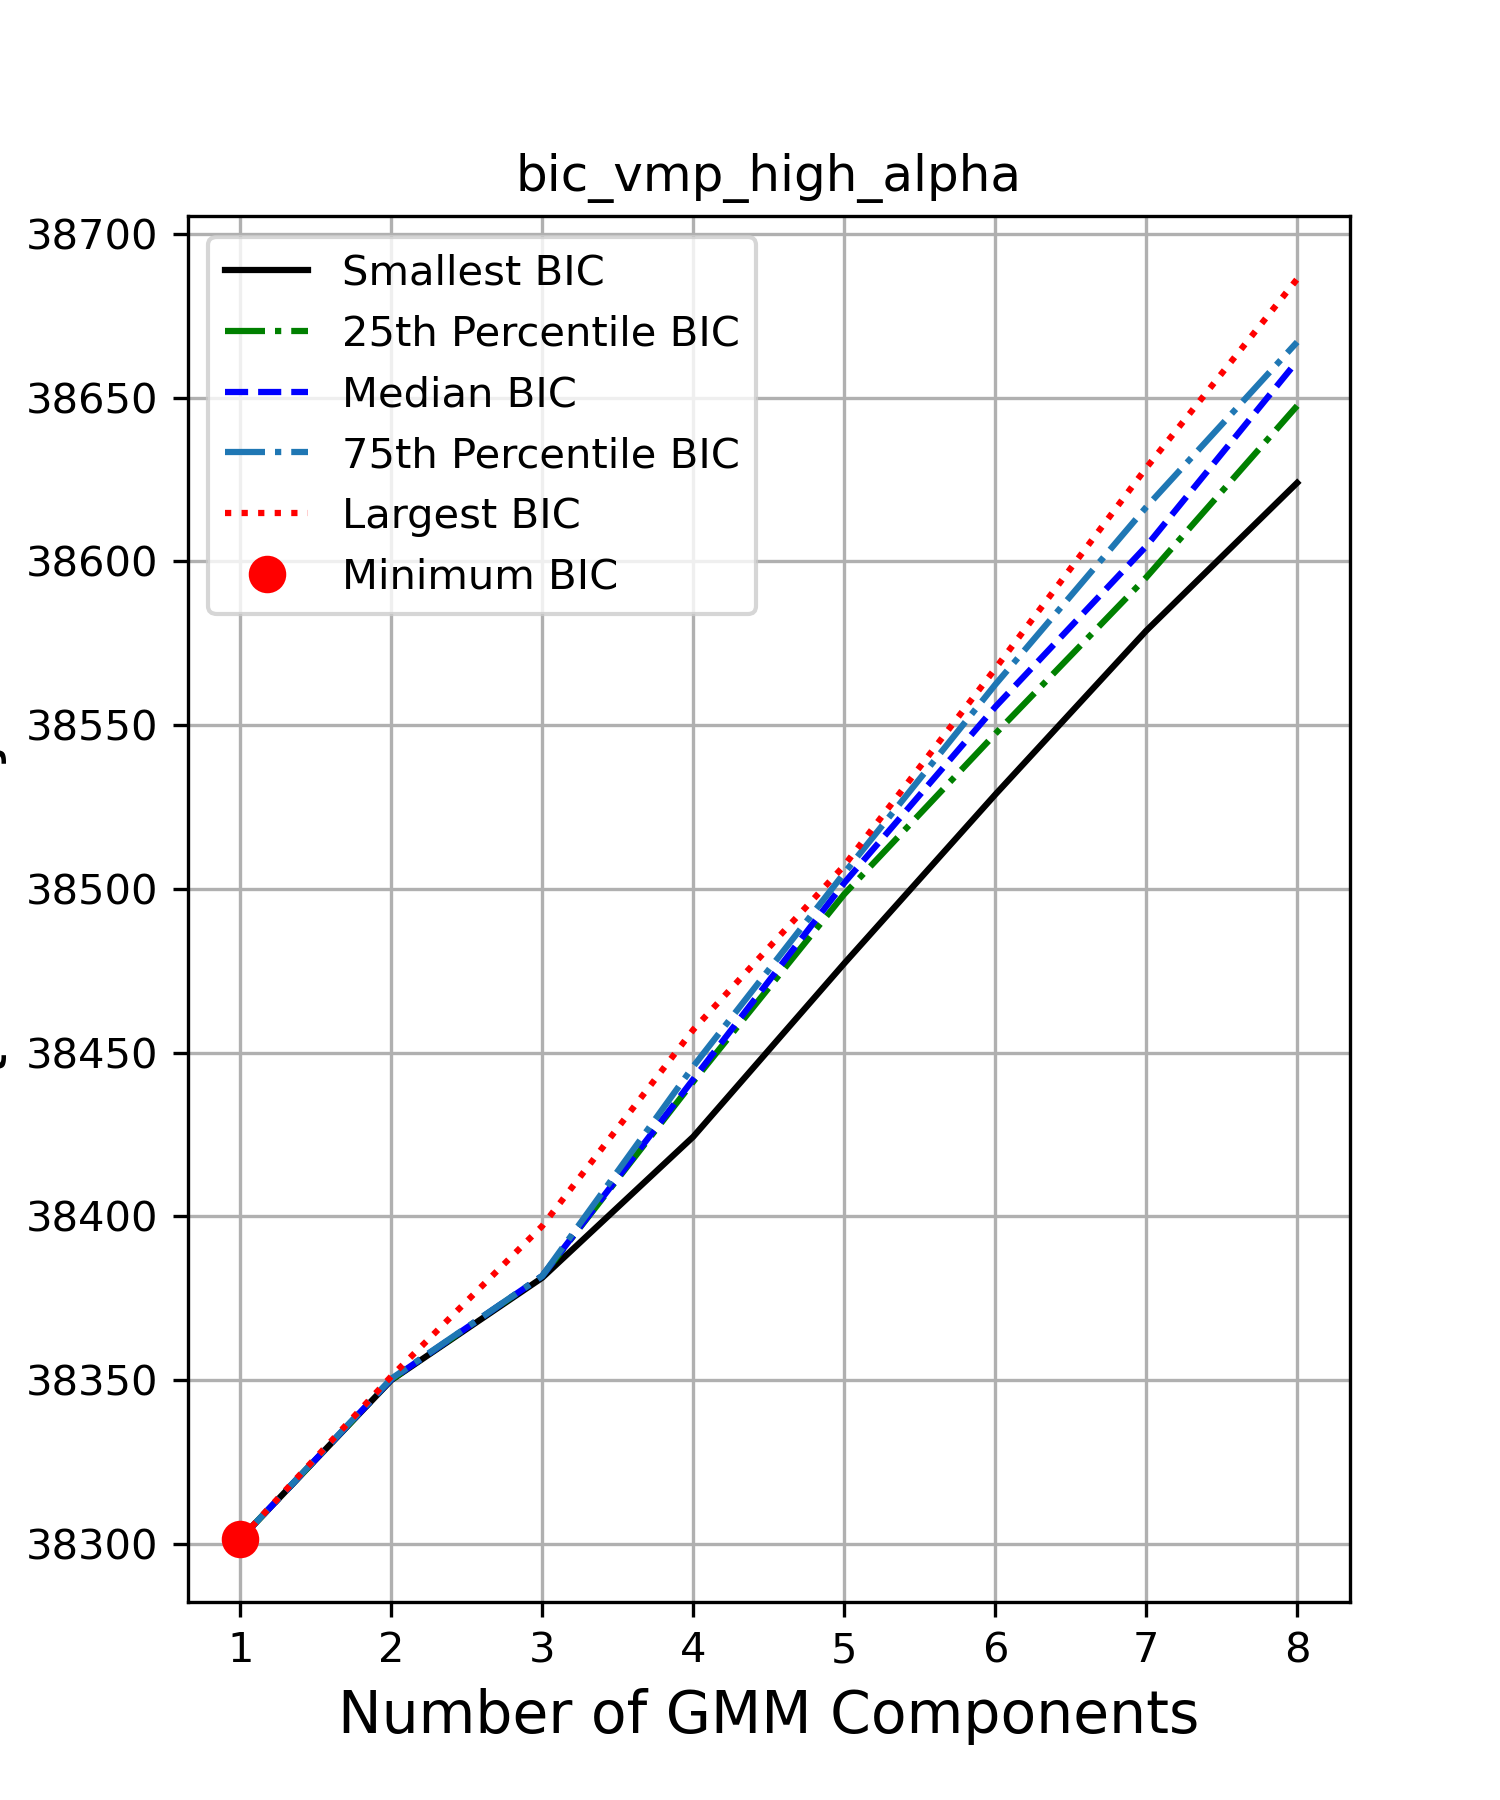
\includegraphics[width=\textwidth]{../figures/bic_vmp_high_alpha.png}
        \caption{High-$\alpha$ VMP}
    \end{subfigure}
    \begin{subfigure}[t]{0.24\textwidth}
        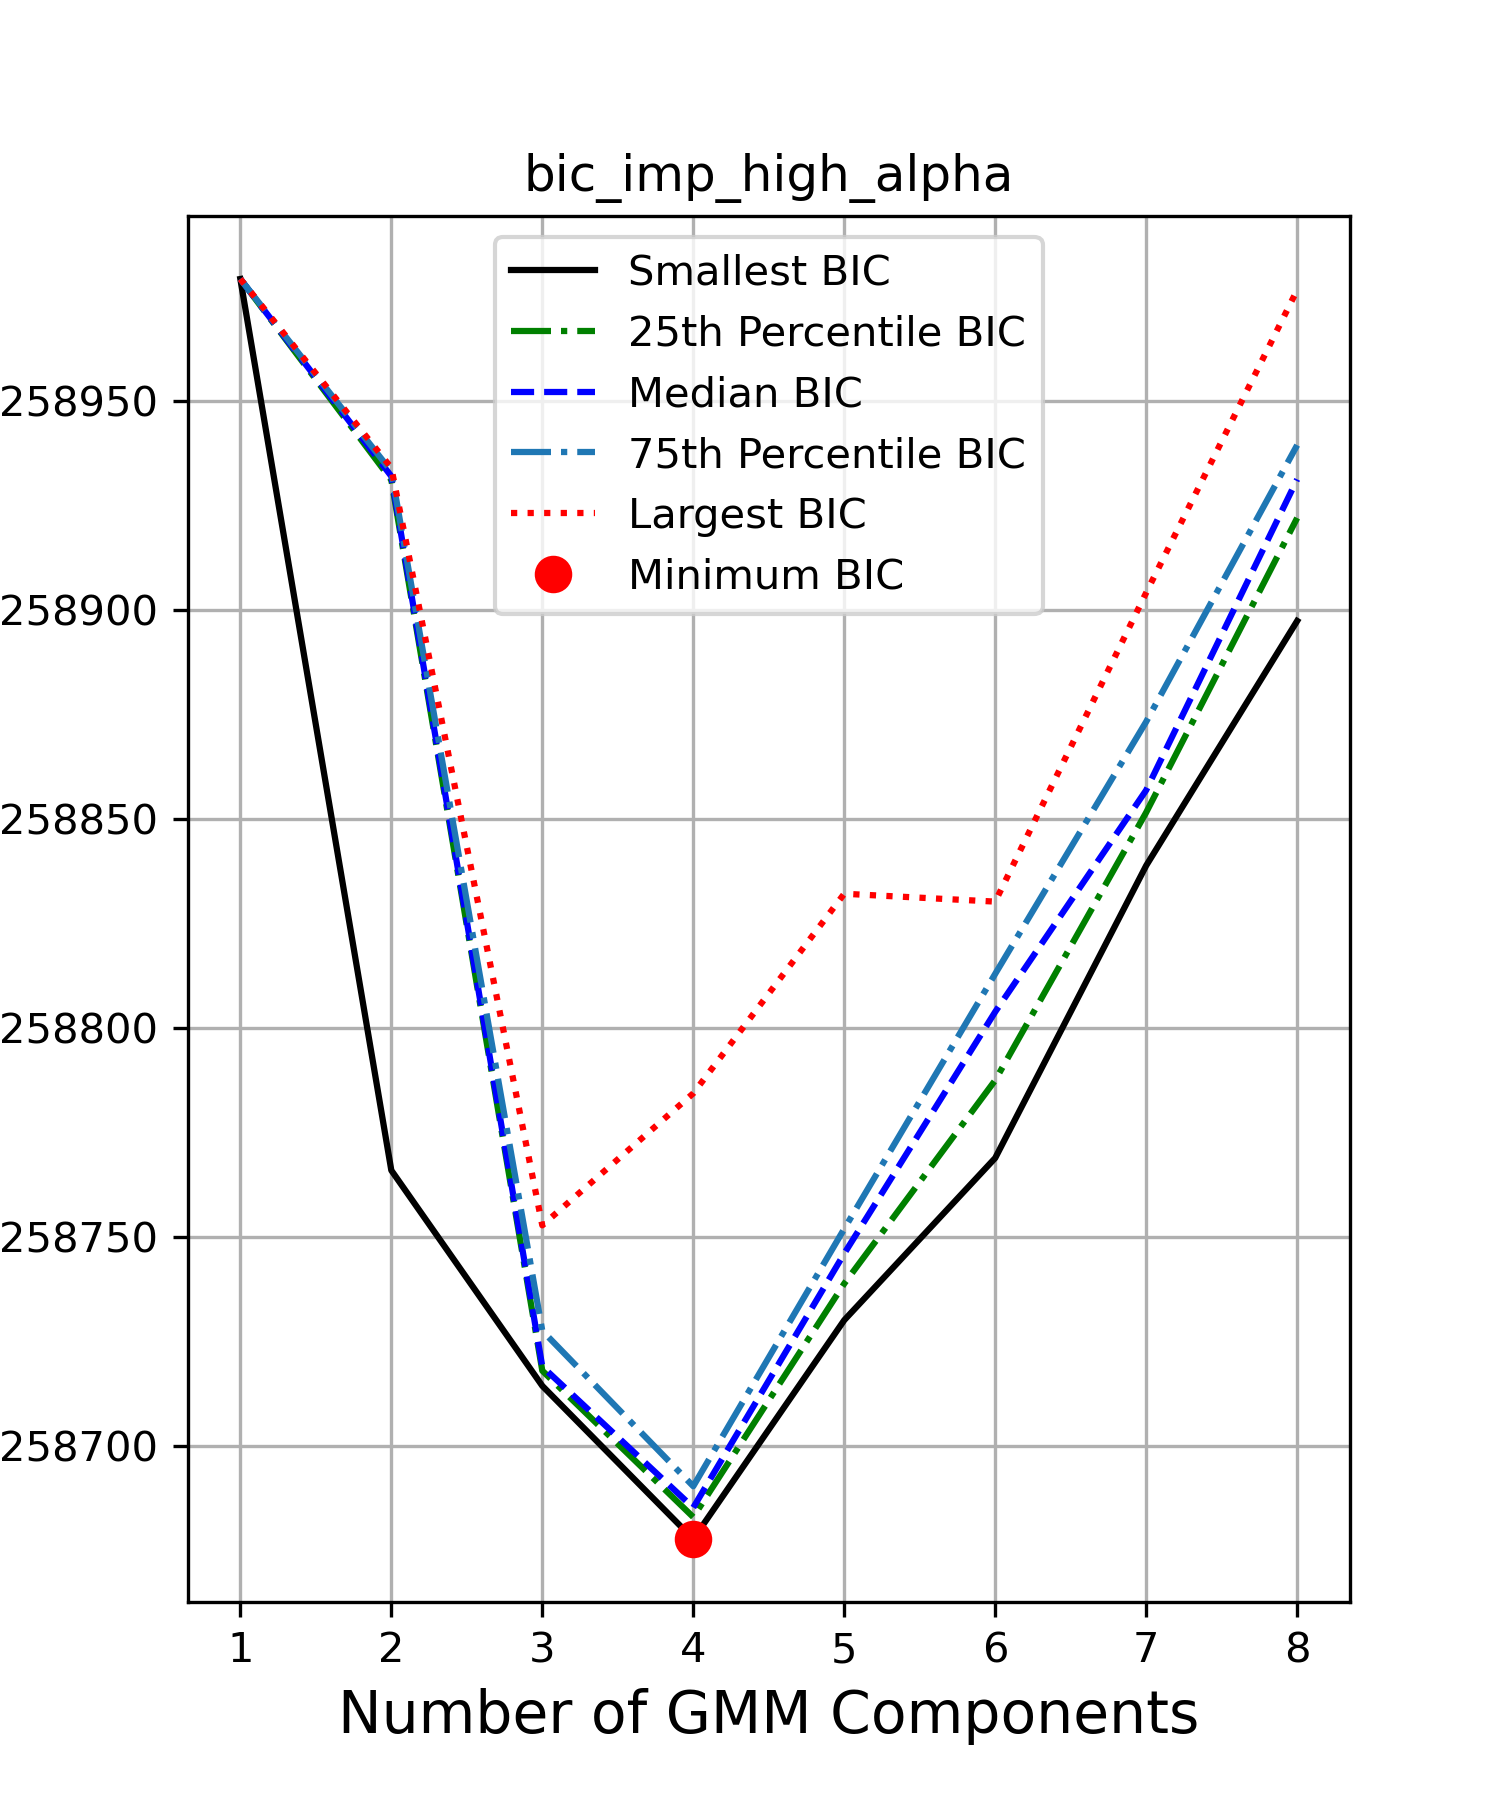
\includegraphics[width=\textwidth]{../figures/bic_imp_high_alpha.png}
        \caption{High-$\alpha$ IMP}
    \end{subfigure}
    \begin{subfigure}[t]{0.24\textwidth}
        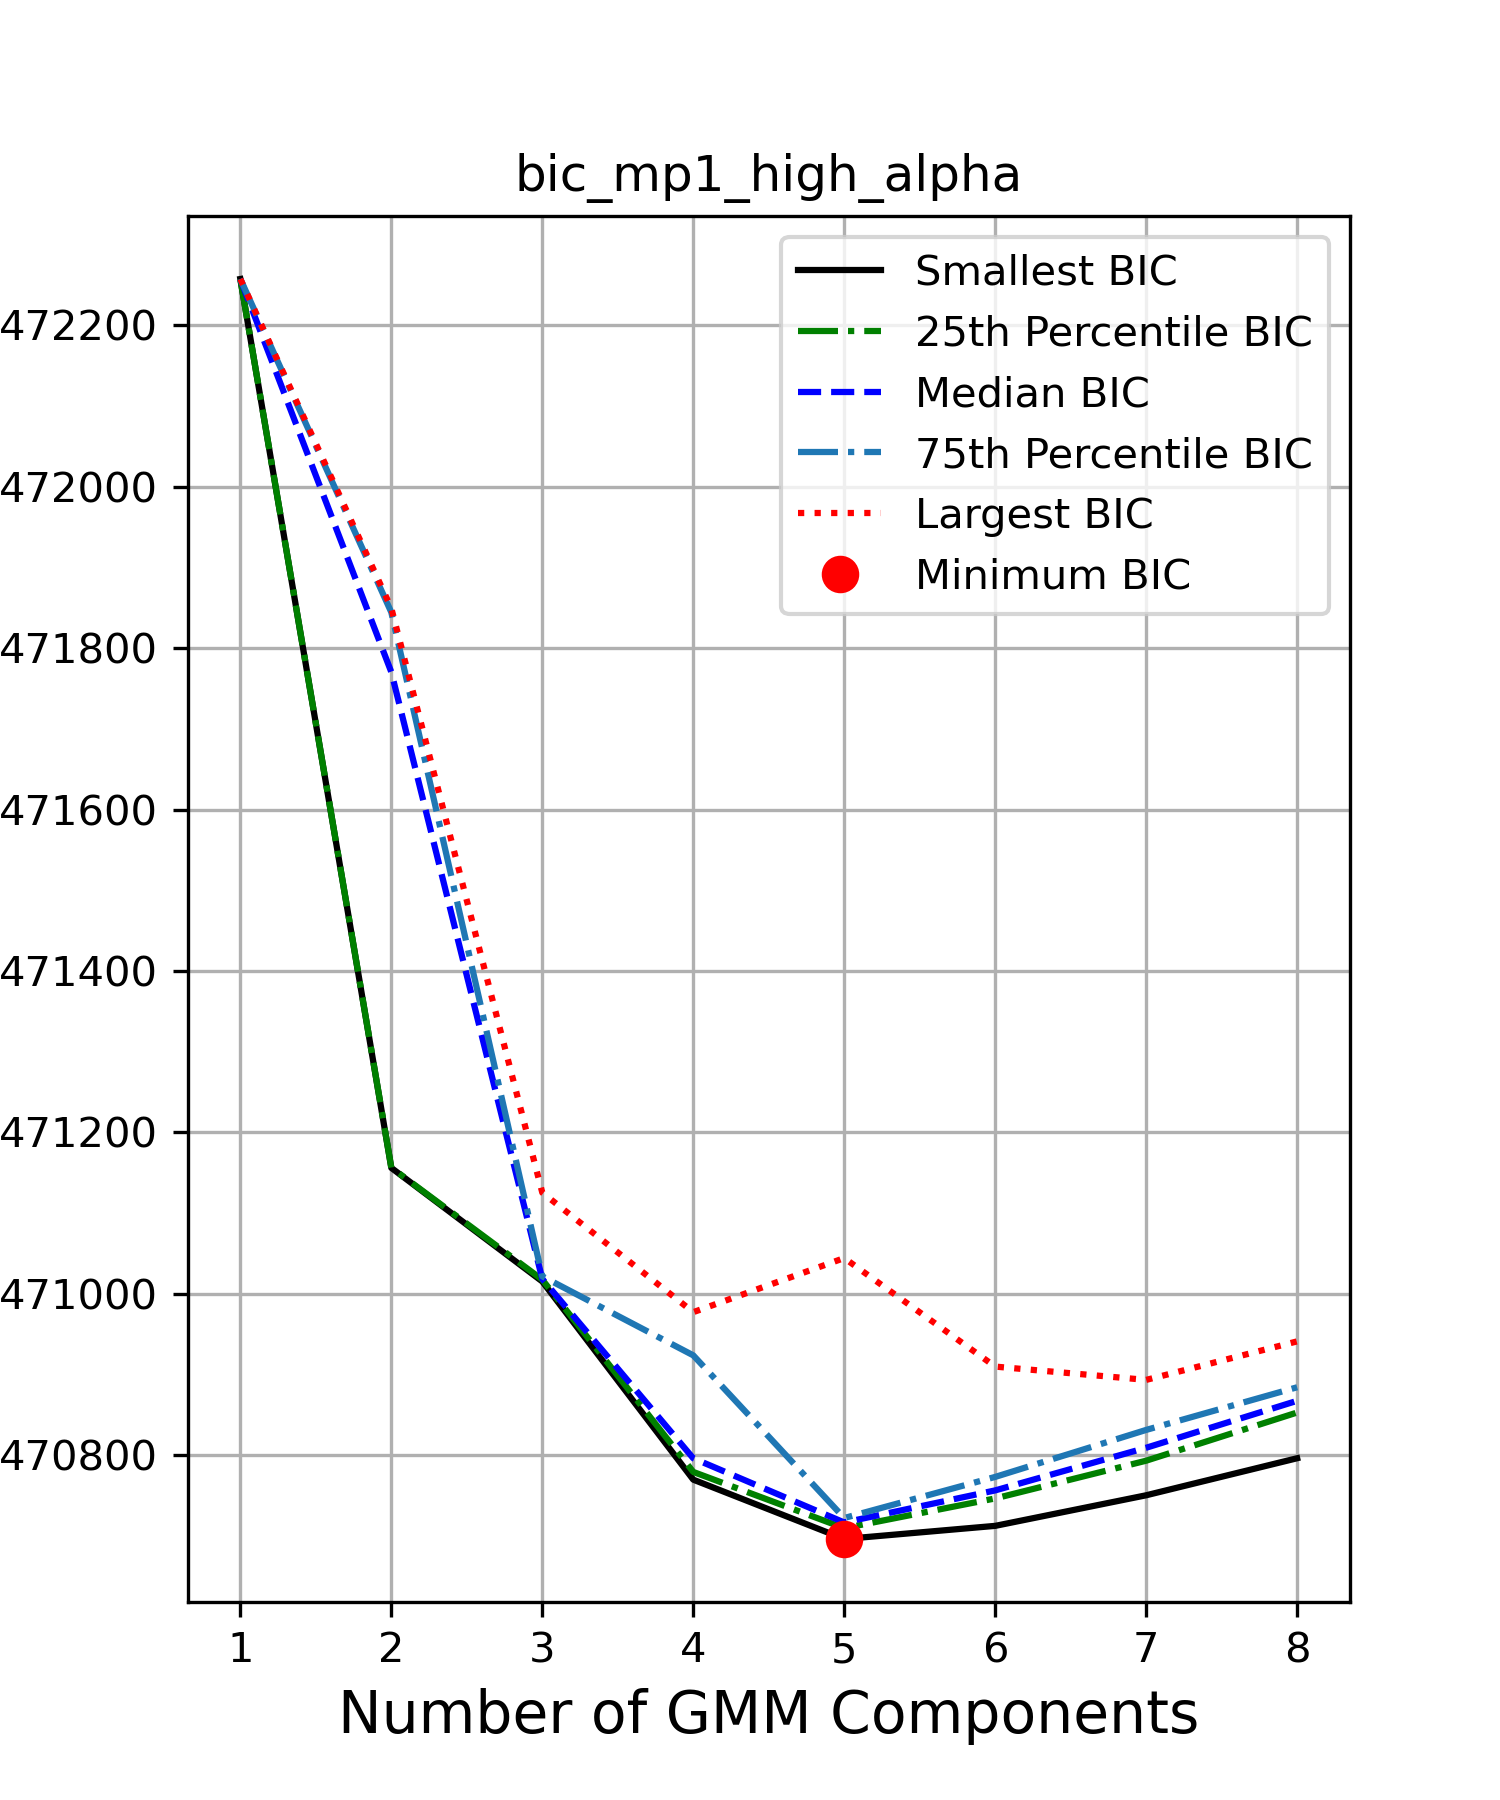
\includegraphics[width=\textwidth]{../figures/bic_mp1_high_alpha.png}
        \caption{High-$\alpha$ MP1}
    \end{subfigure}
    \begin{subfigure}[t]{0.24\textwidth}
        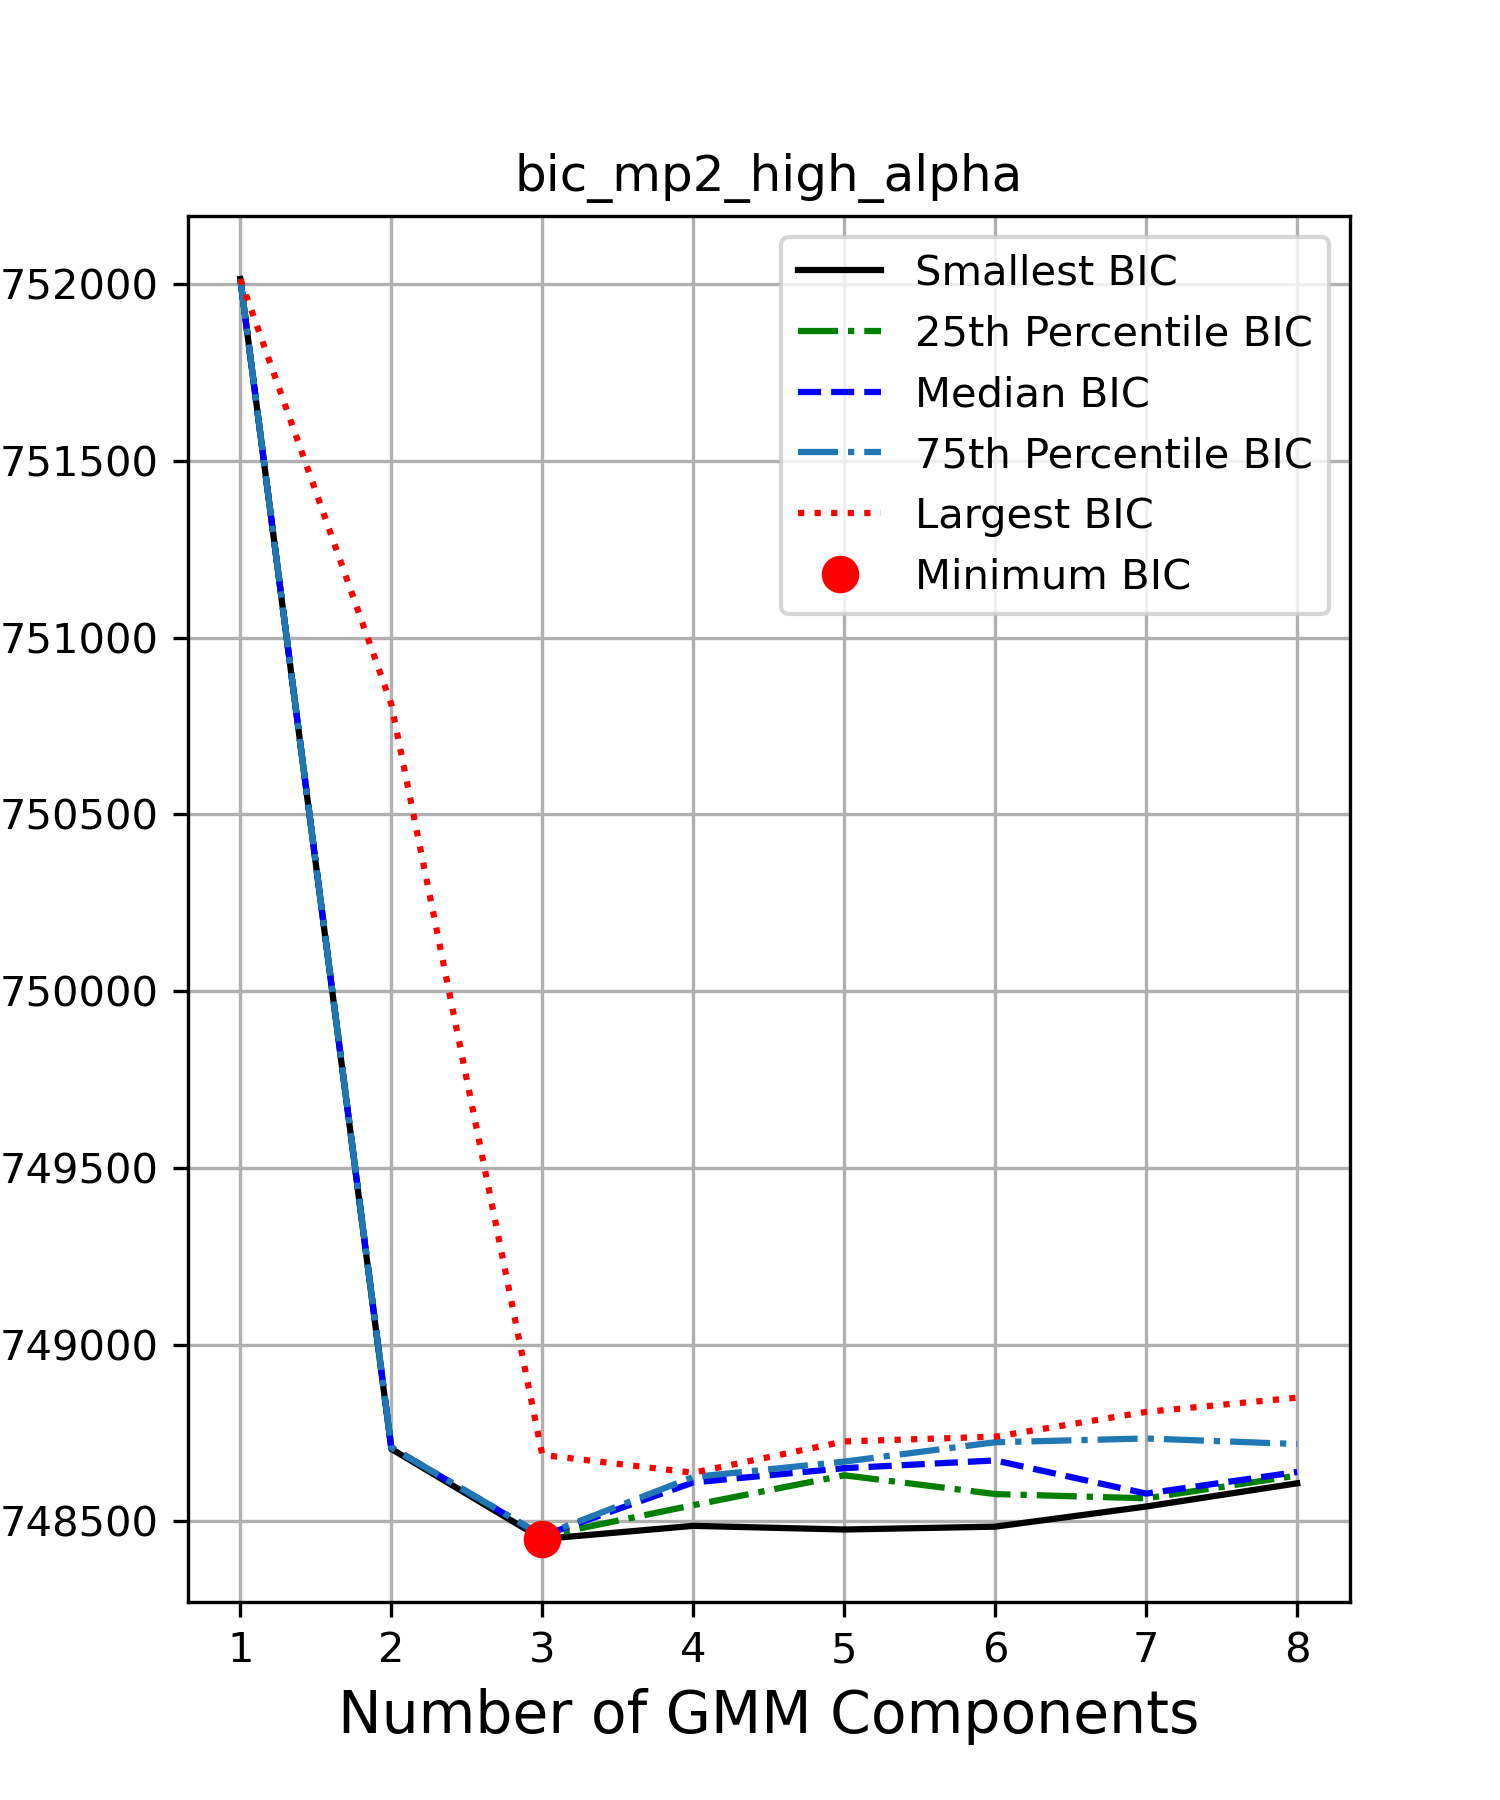
\includegraphics[width=\textwidth]{../figures/bic_mp2_high_alpha.png}
        \caption{High-$\alpha$ MP2}
    \end{subfigure}

    \vspace{0.5em}

    % Low-alpha row
    \begin{subfigure}[t]{0.24\textwidth}
        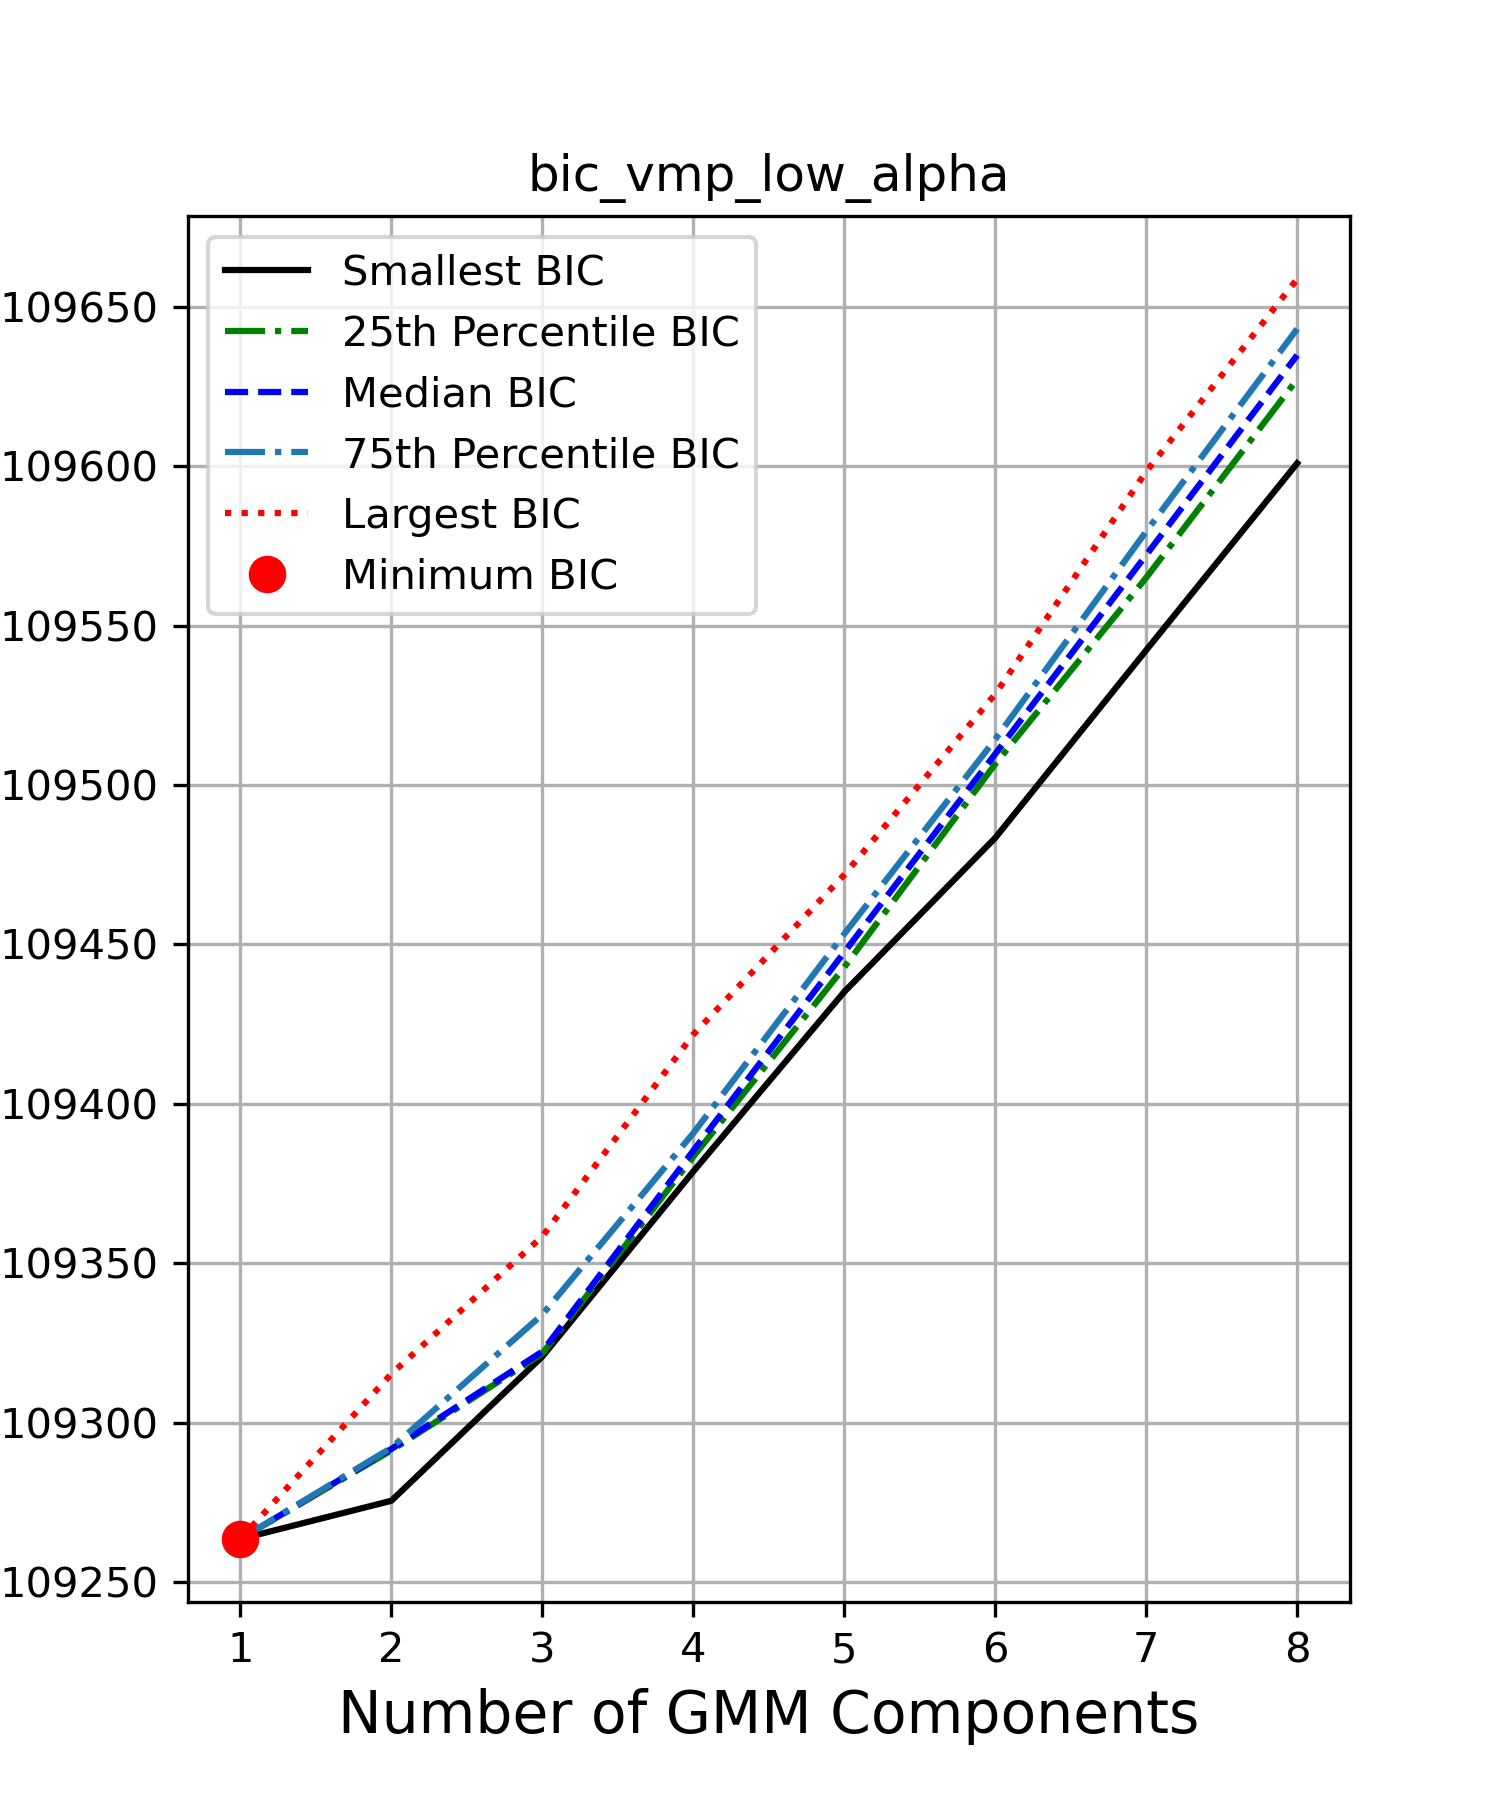
\includegraphics[width=\textwidth]{../figures/bic_vmp_low_alpha.png}
        \caption{Low-$\alpha$ VMP}
    \end{subfigure}
    \begin{subfigure}[t]{0.24\textwidth}
        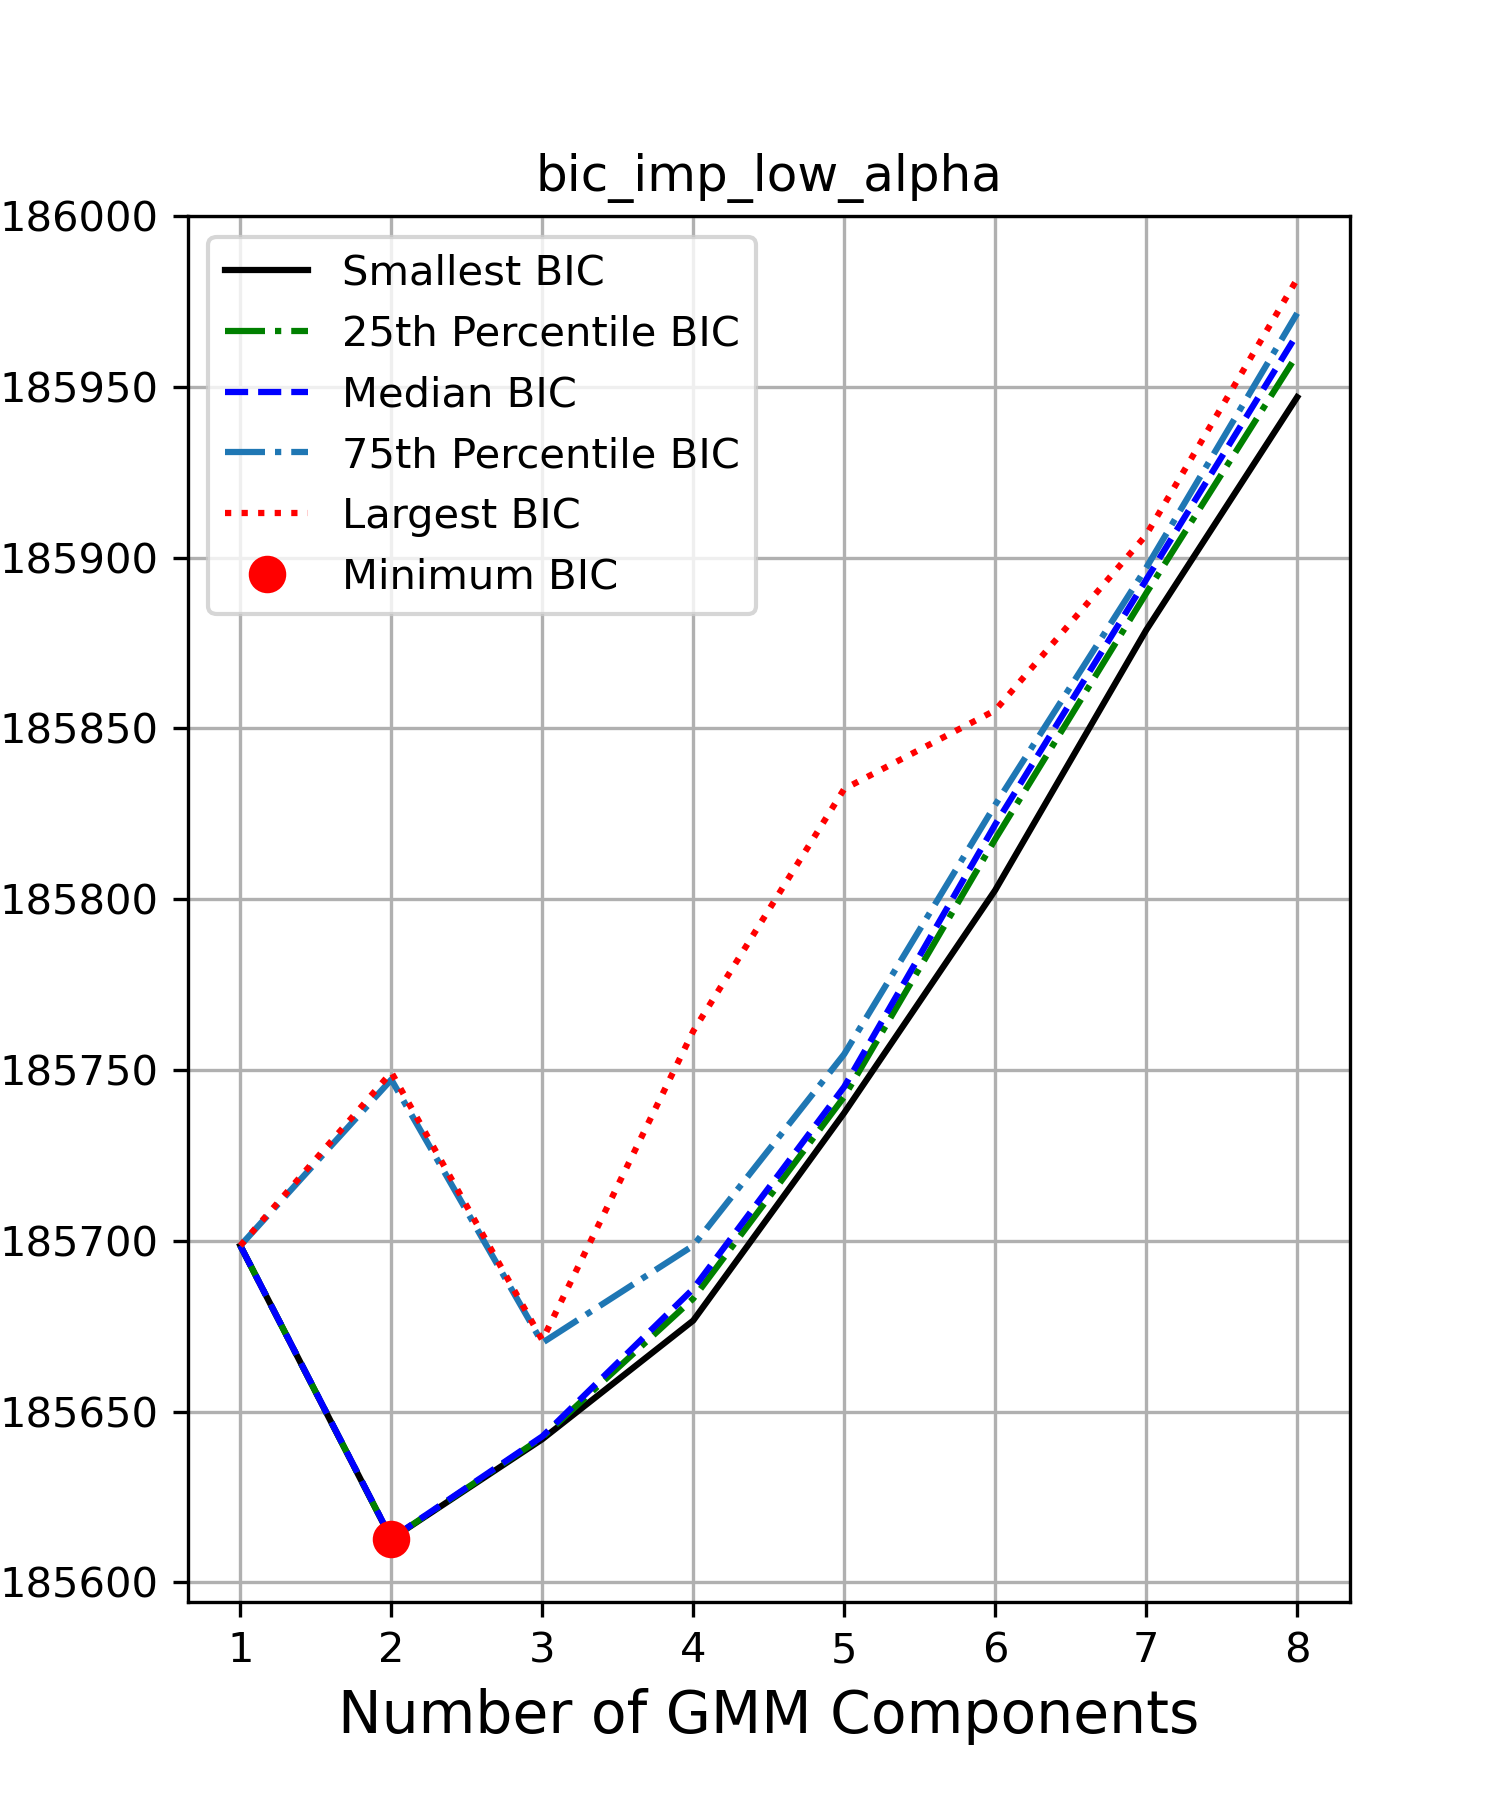
\includegraphics[width=\textwidth]{../figures/bic_imp_low_alpha.png}
        \caption{Low-$\alpha$ IMP}
    \end{subfigure}
    \begin{subfigure}[t]{0.24\textwidth}
        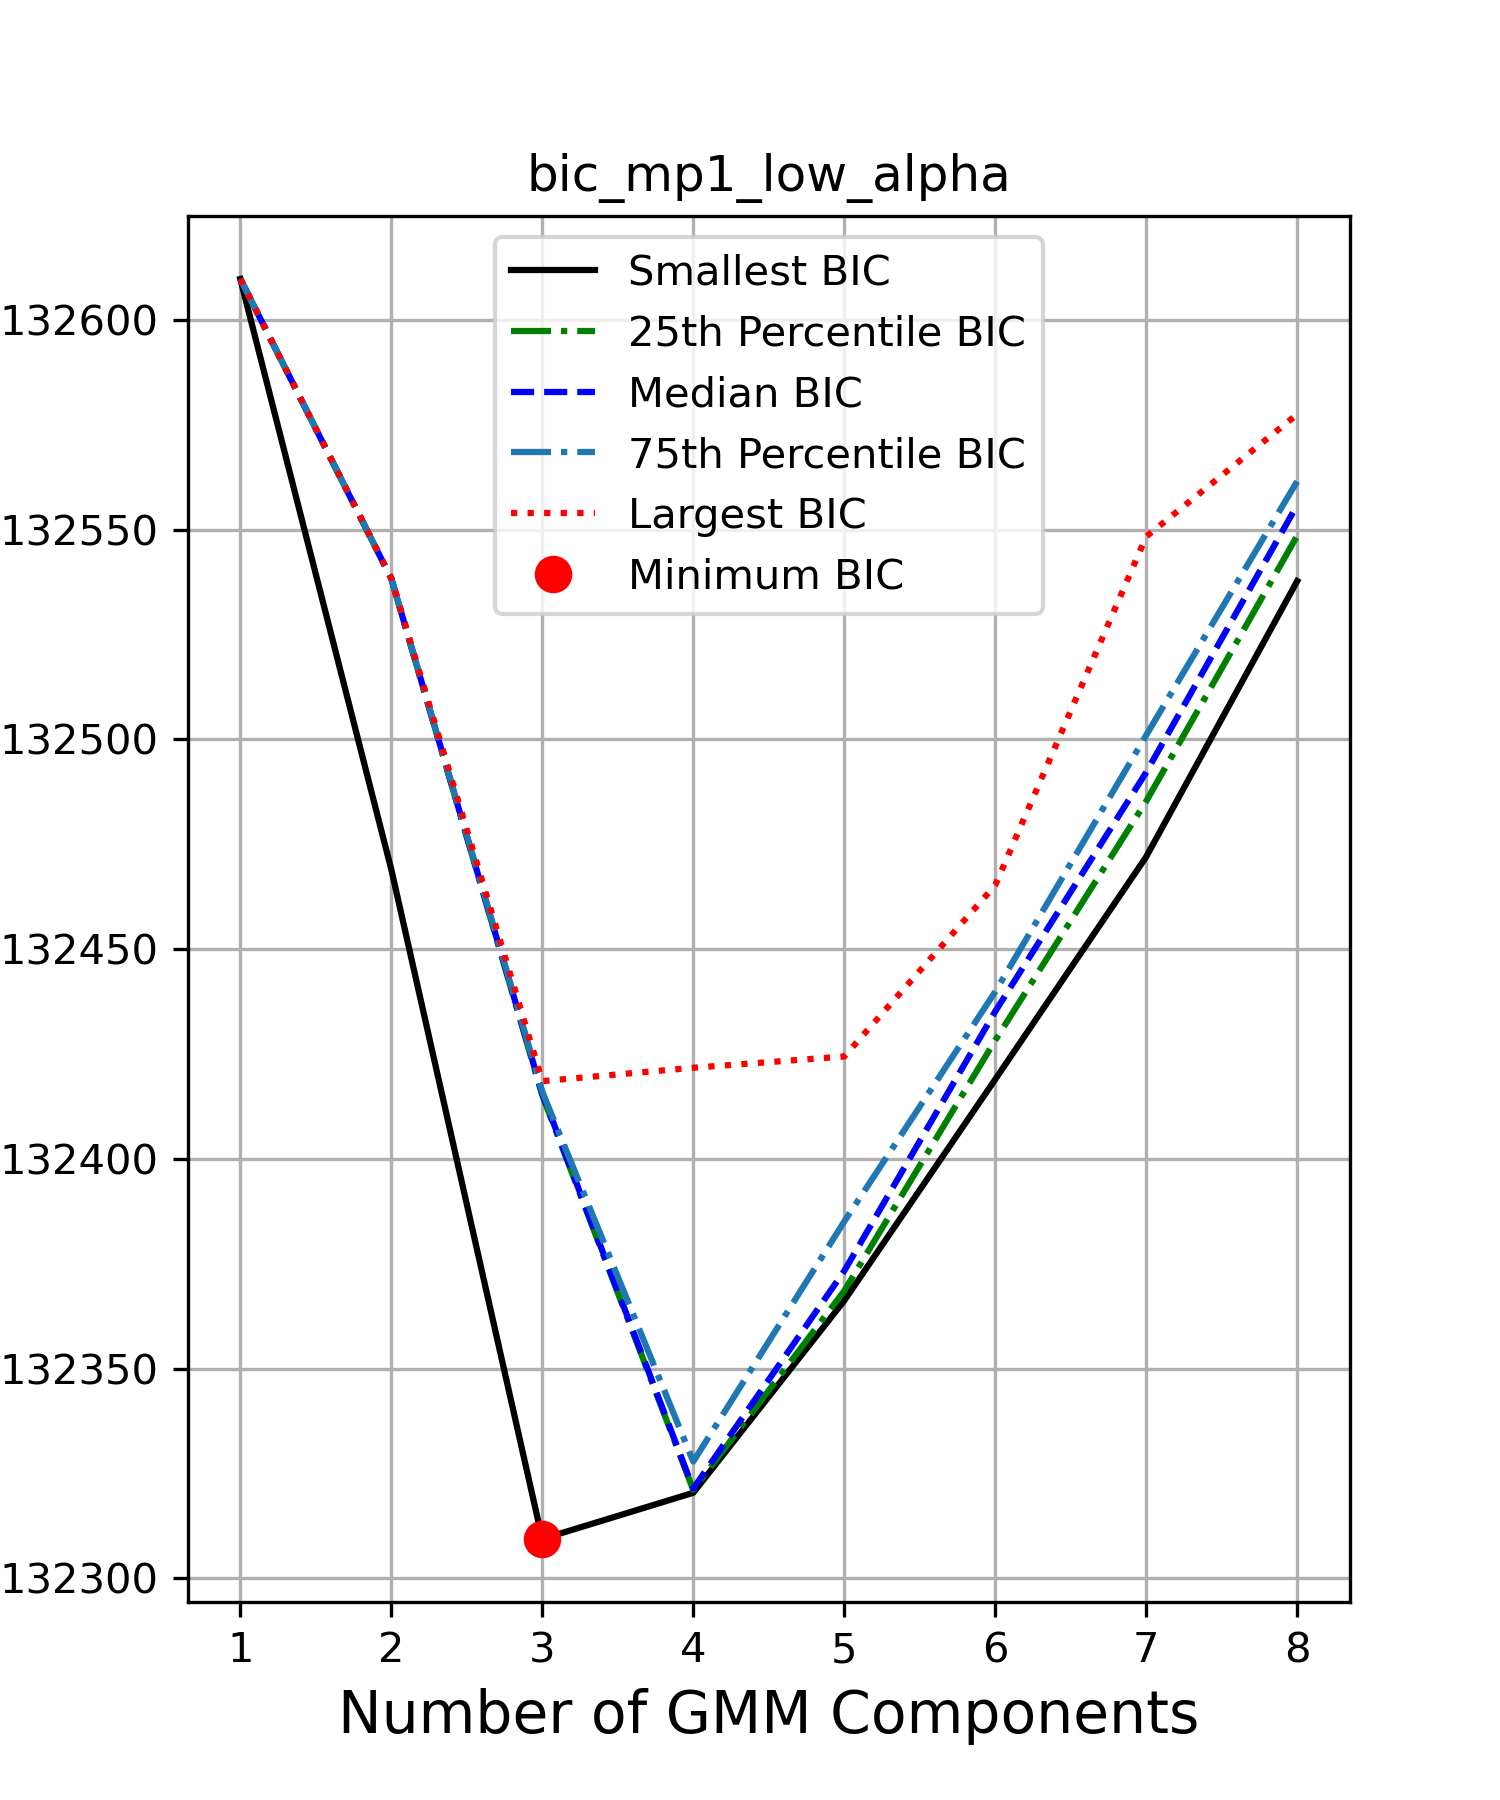
\includegraphics[width=\textwidth]{../figures/bic_mp1_low_alpha.png}
        \caption{Low-$\alpha$ MP1}
    \end{subfigure}
    \begin{subfigure}[t]{0.24\textwidth}
        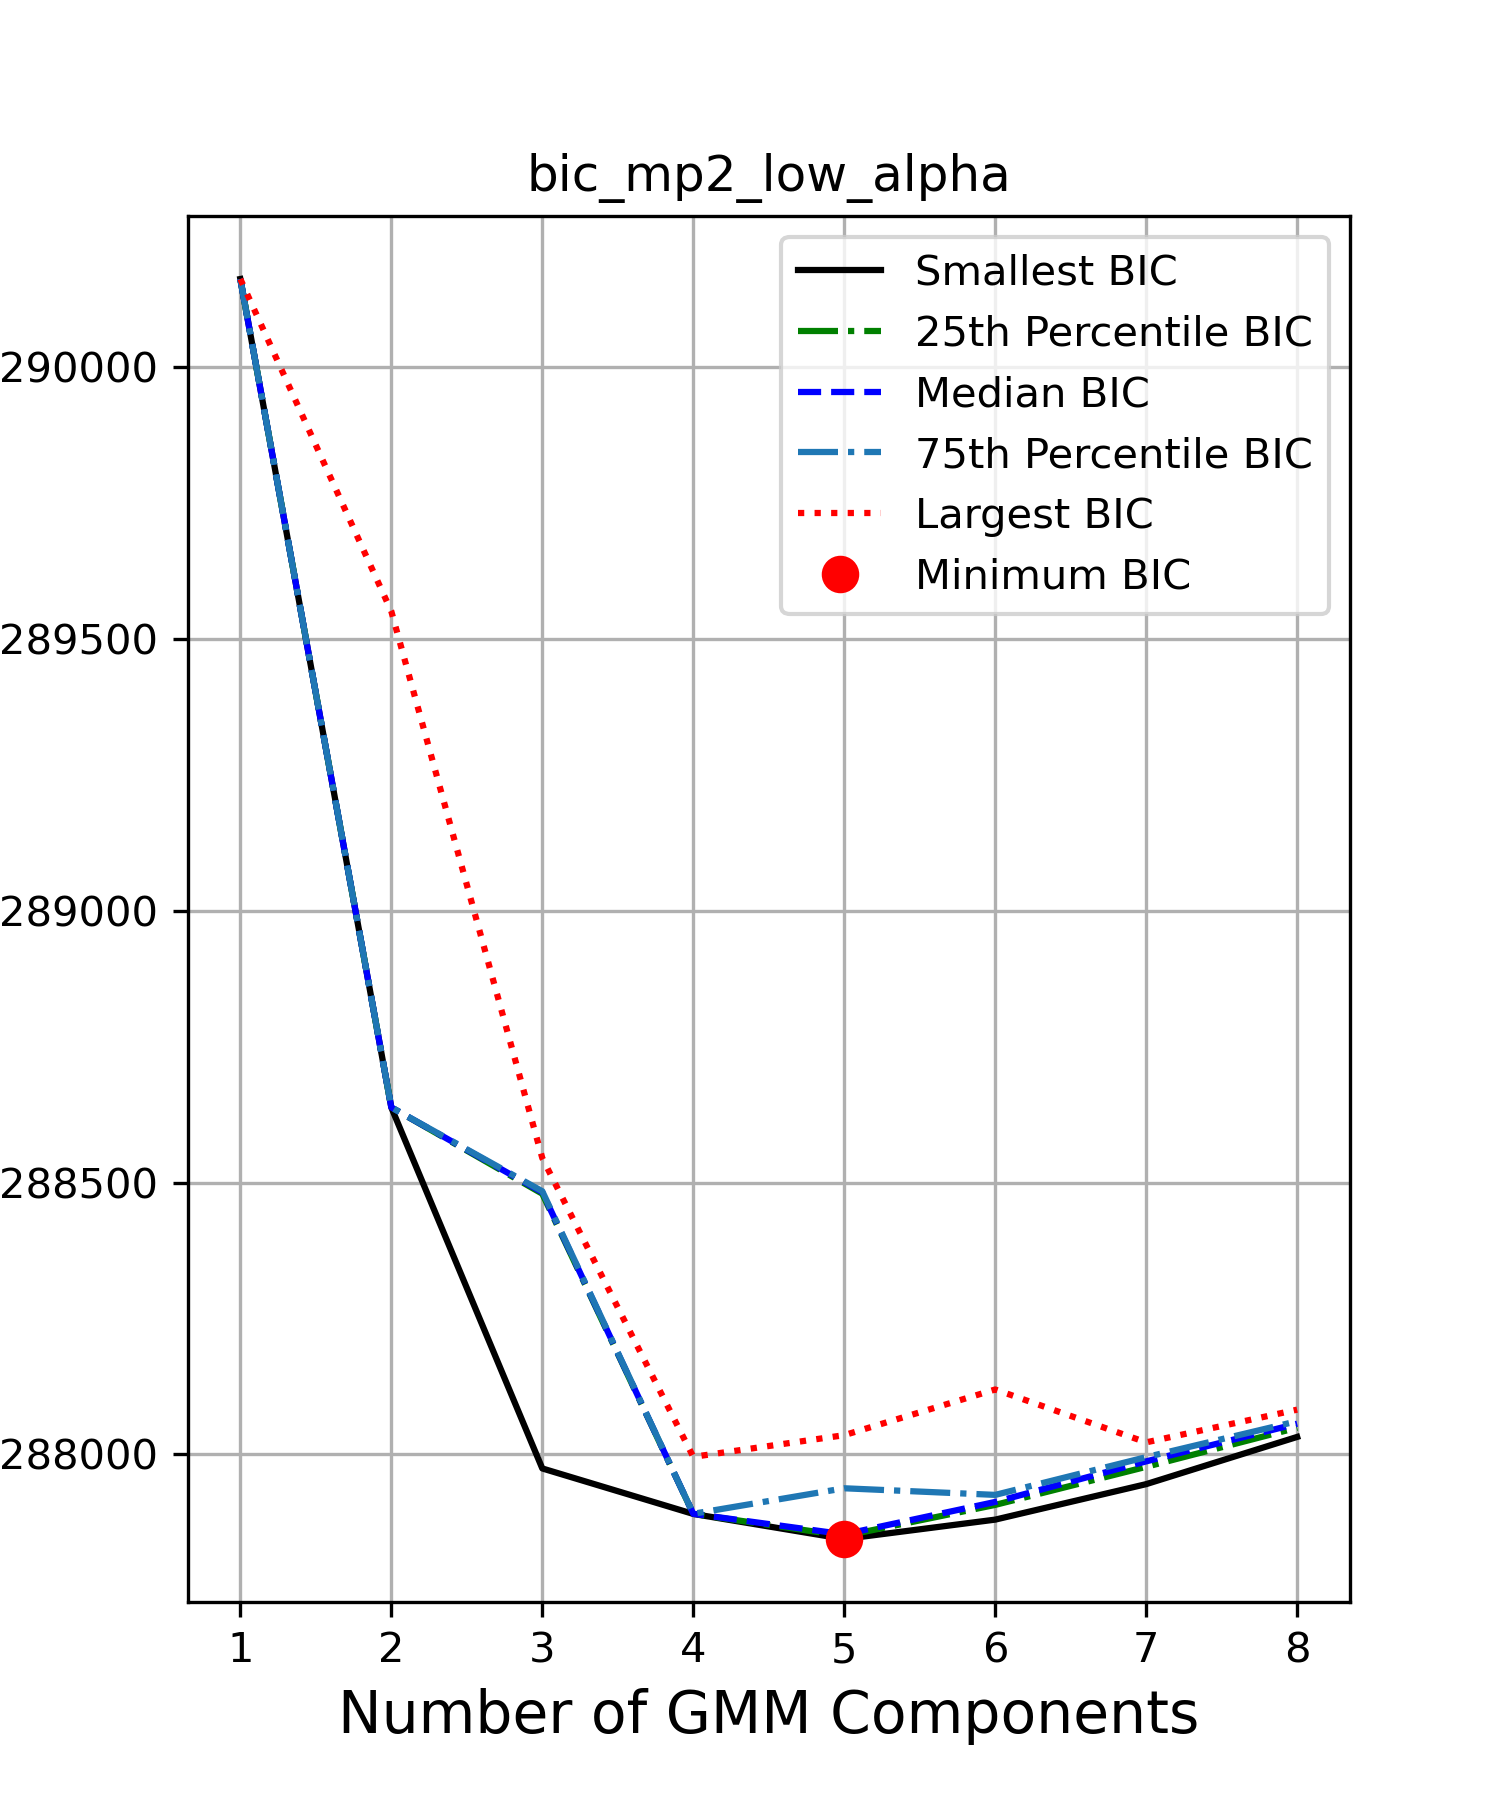
\includegraphics[width=\textwidth]{../figures/bic_mp2_low_alpha.png}
        \caption{Low-$\alpha$ MP2}
    \end{subfigure}

    \caption{BIC scores for different metallicity bins, grouped by high- and low-$\alpha$ populations.}
    \label{fig:bic_grid}
\end{figure*}


\subsection{High alpha Gaussian Mixture Model Fit}

\begin{figure}[H]
  \centering

  \begin{subfigure}{0.245\linewidth}
    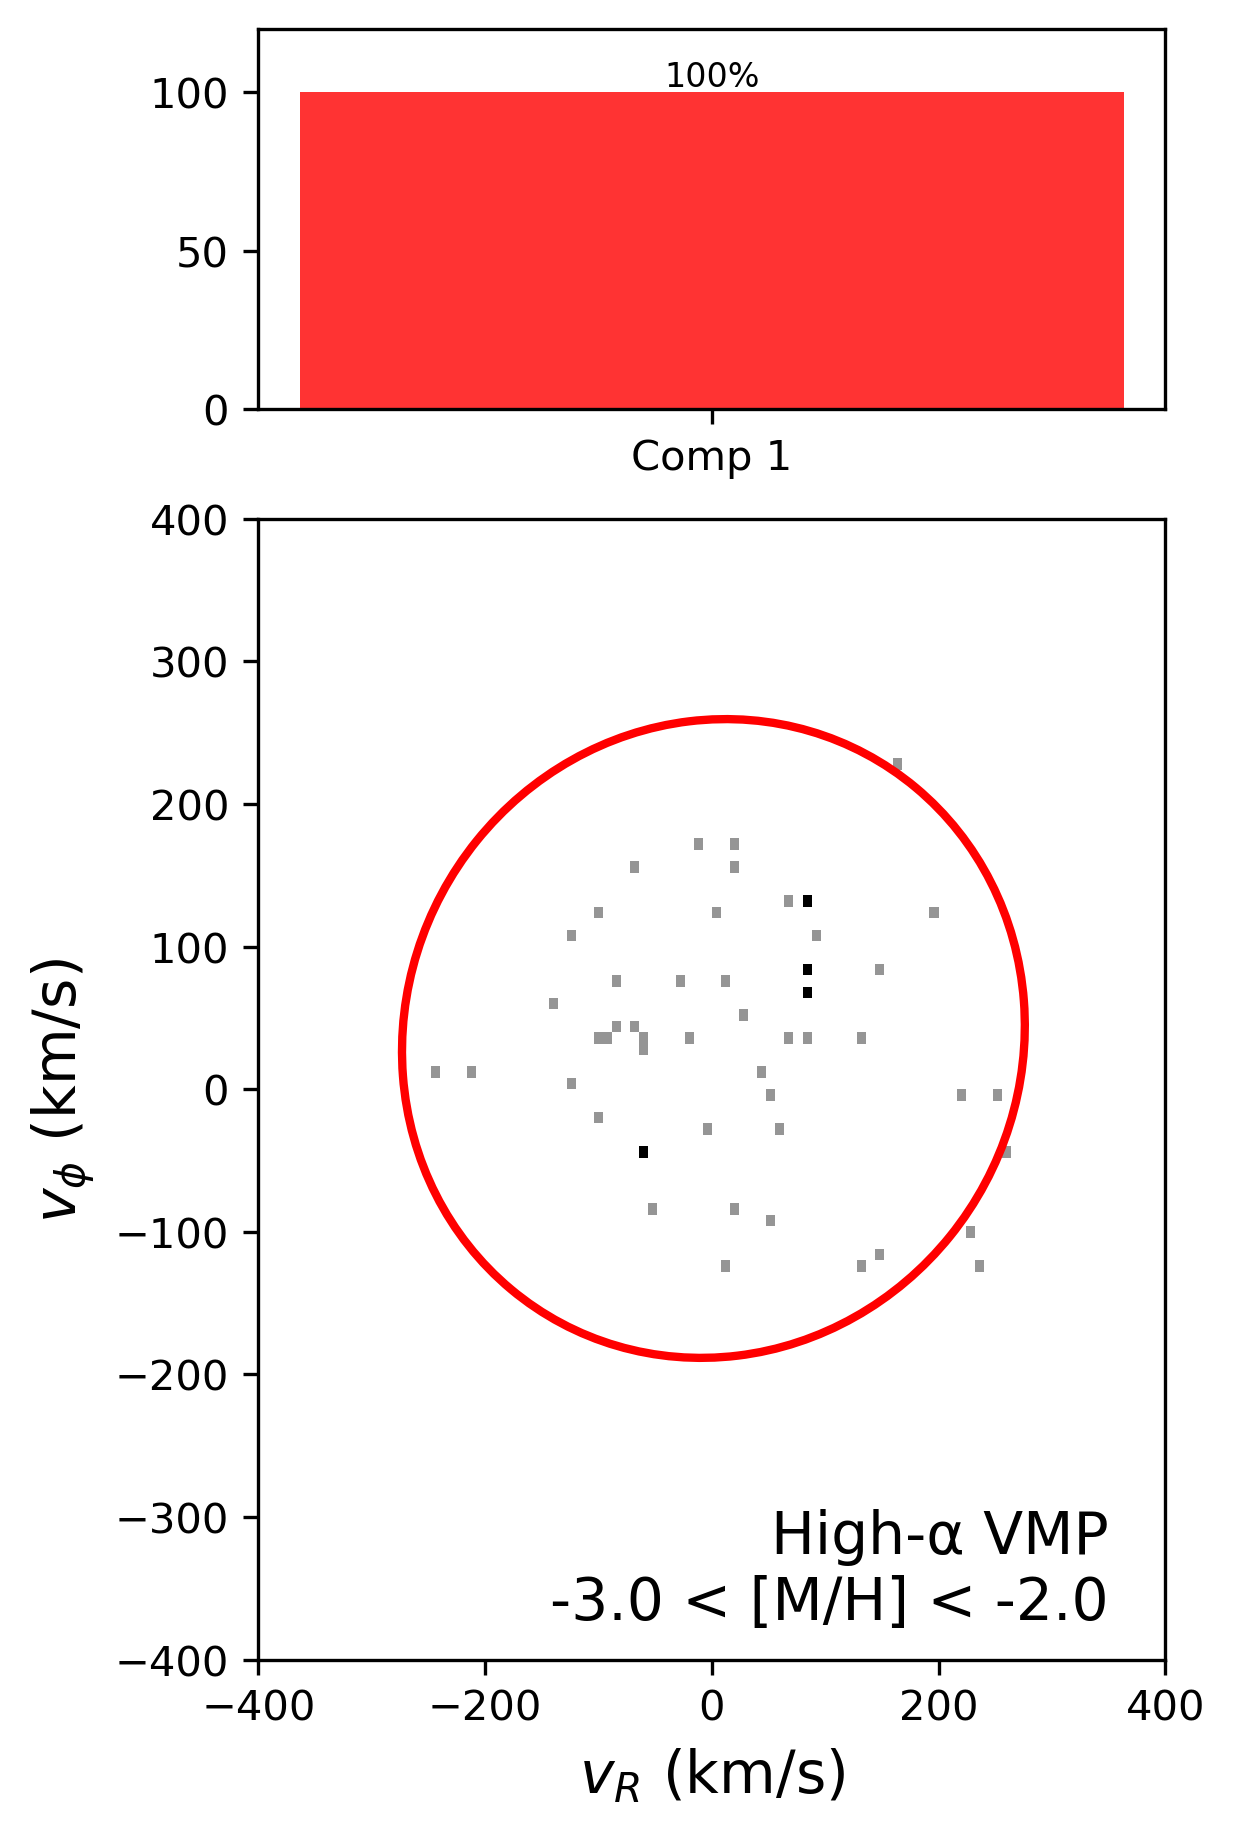
\includegraphics[width=\linewidth]{../figures/gmm_vmp_high_alpha_k1.png}
    \caption{\href{https://raw.githack.com/raunaq-rai/Disentangling-the-Milky-Way-using-GMM/main/figures/VMP\_high\_\_\_-3\%5BM\_H\%5D-2.html}{VMP}}
    \label{fig:vmp_hi}
  \end{subfigure}\hfill
  \begin{subfigure}{0.245\linewidth}
    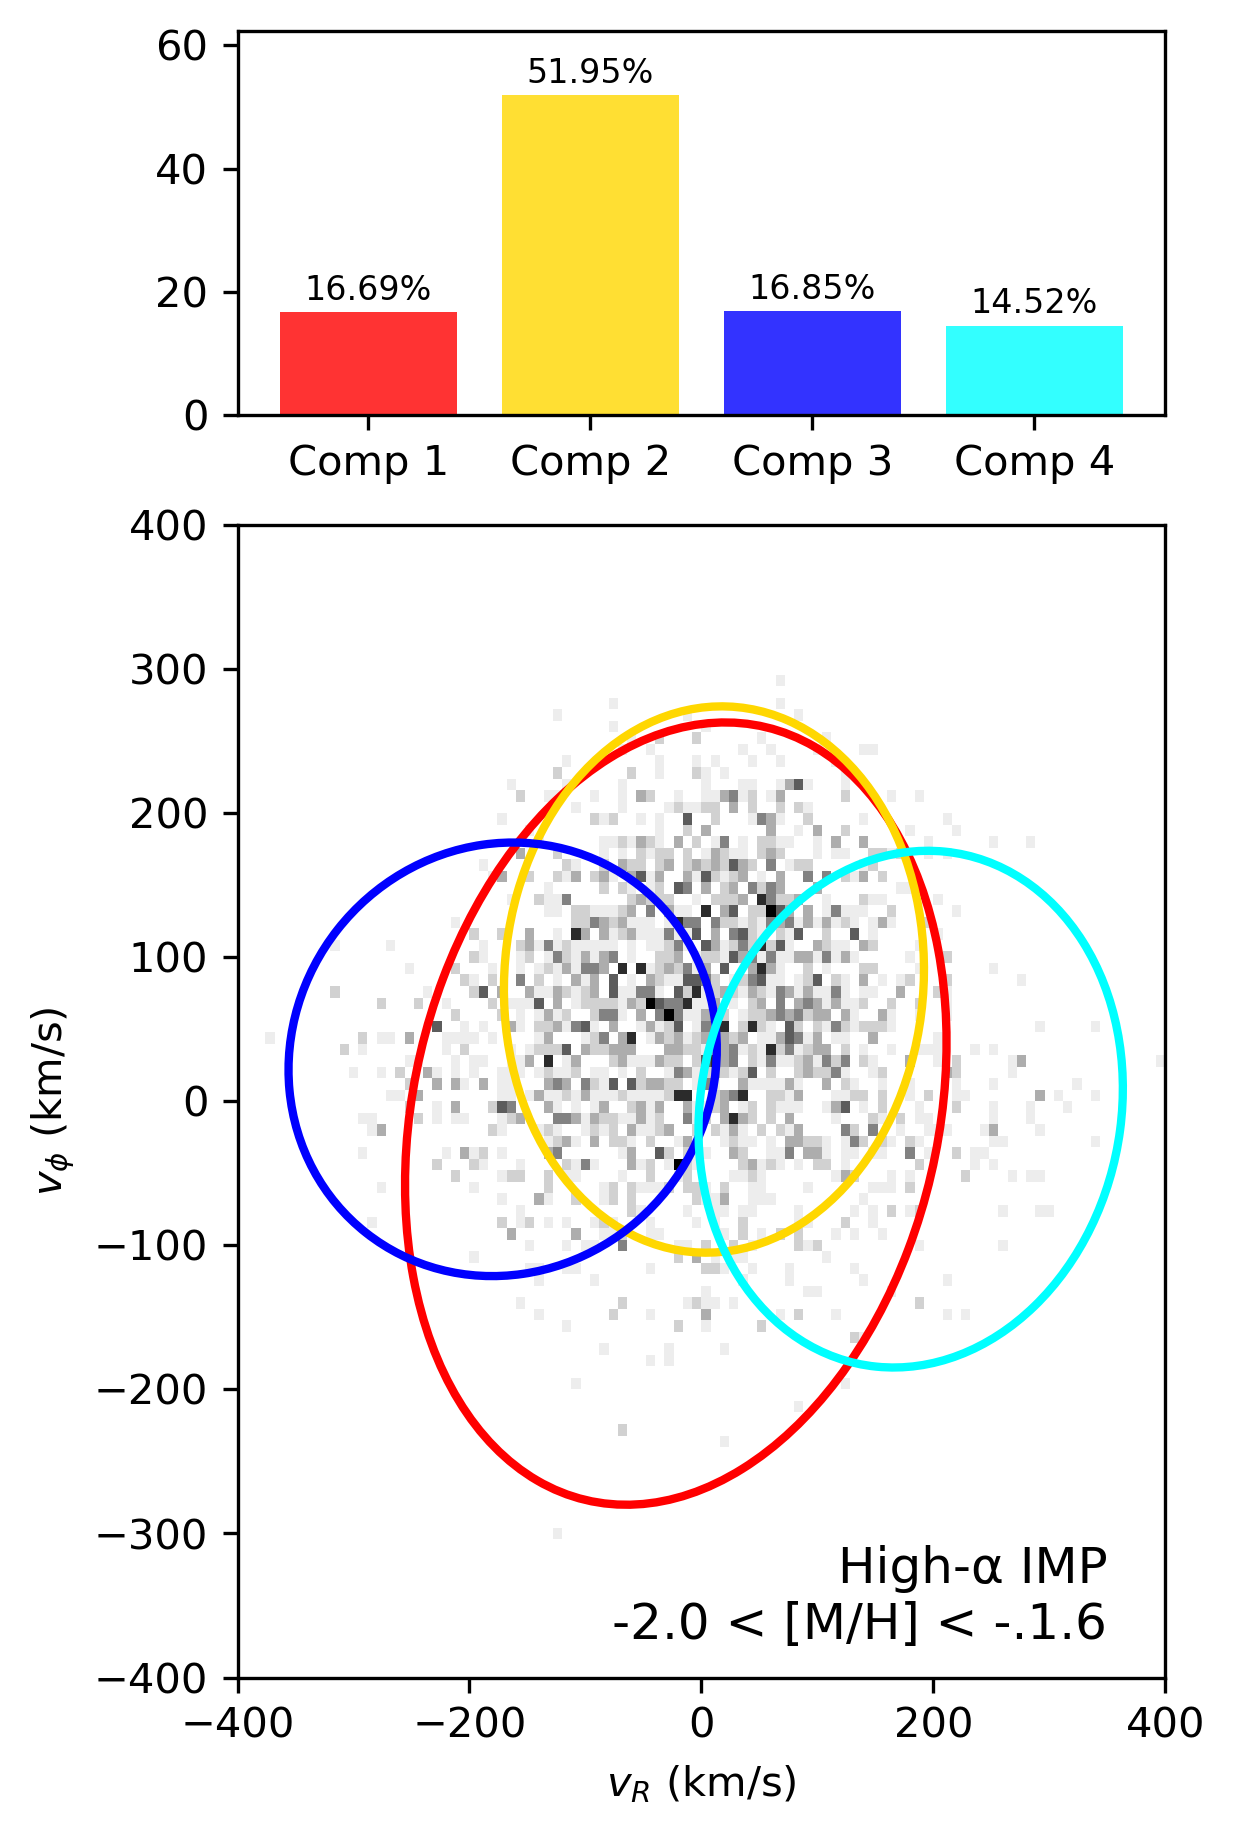
\includegraphics[width=\linewidth]{../figures/gmm_imp_high_alpha_k4.png}
    \caption{\href{https://raw.githack.com/raunaq-rai/Disentangling-the-Milky-Way-using-GMM/main/figures/IMP\_high\_\_\_-2\%5BM\_H\%5D-1.6.html}{IMP}}
    \label{fig:imp_hi}
  \end{subfigure}\hfill
  \begin{subfigure}{0.245\linewidth}
    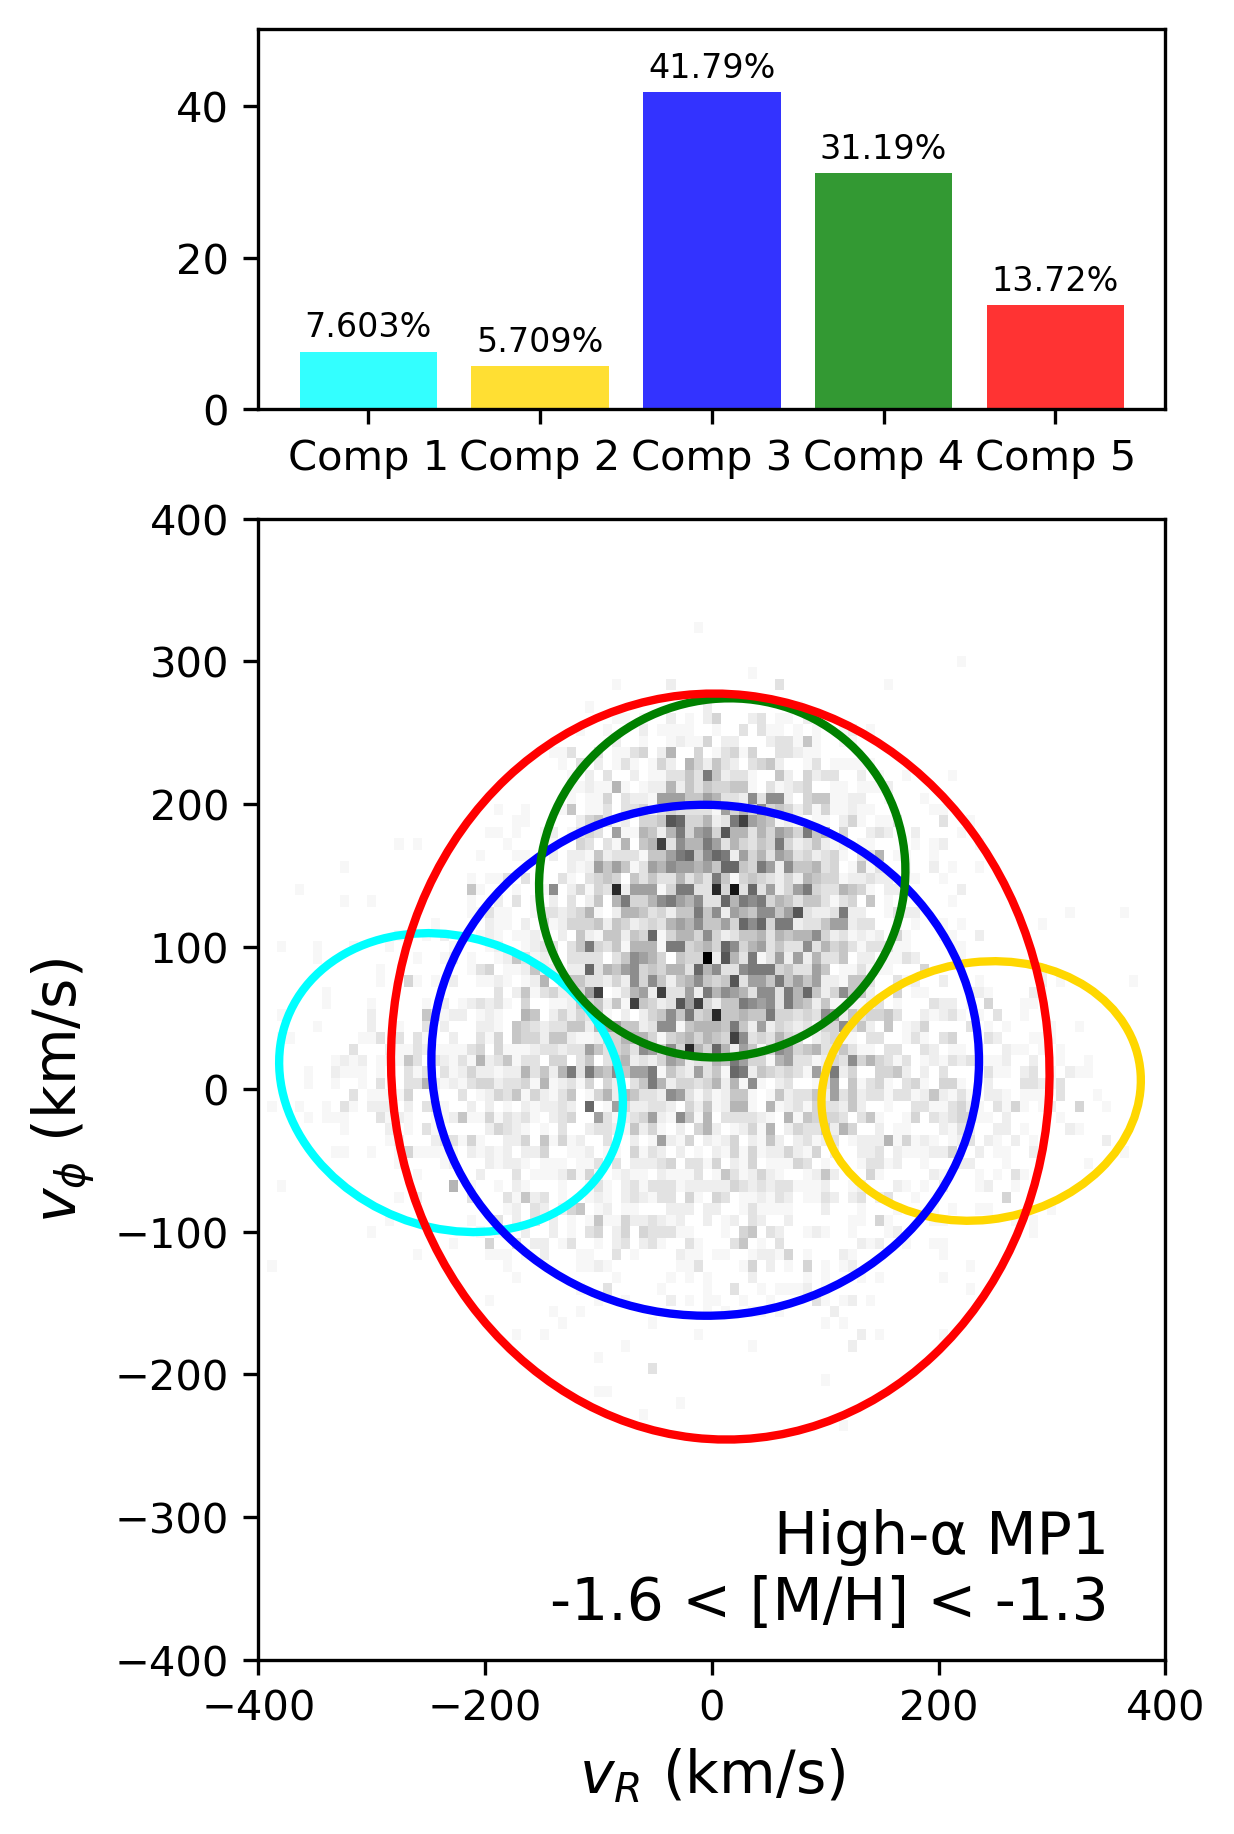
\includegraphics[width=\linewidth]{../figures/gmm_mp1_high_alpha_k5.png}
    \caption{\href{https://raw.githack.com/raunaq-rai/Disentangling-the-Milky-Way-using-GMM/main/figures/MP1\_high\_\_\_-1.6\%5BM\_H\%5D-1.3.html}{MP1}}
    \label{fig:mp1_hi}
  \end{subfigure}\hfill
  \begin{subfigure}{0.245\linewidth}
    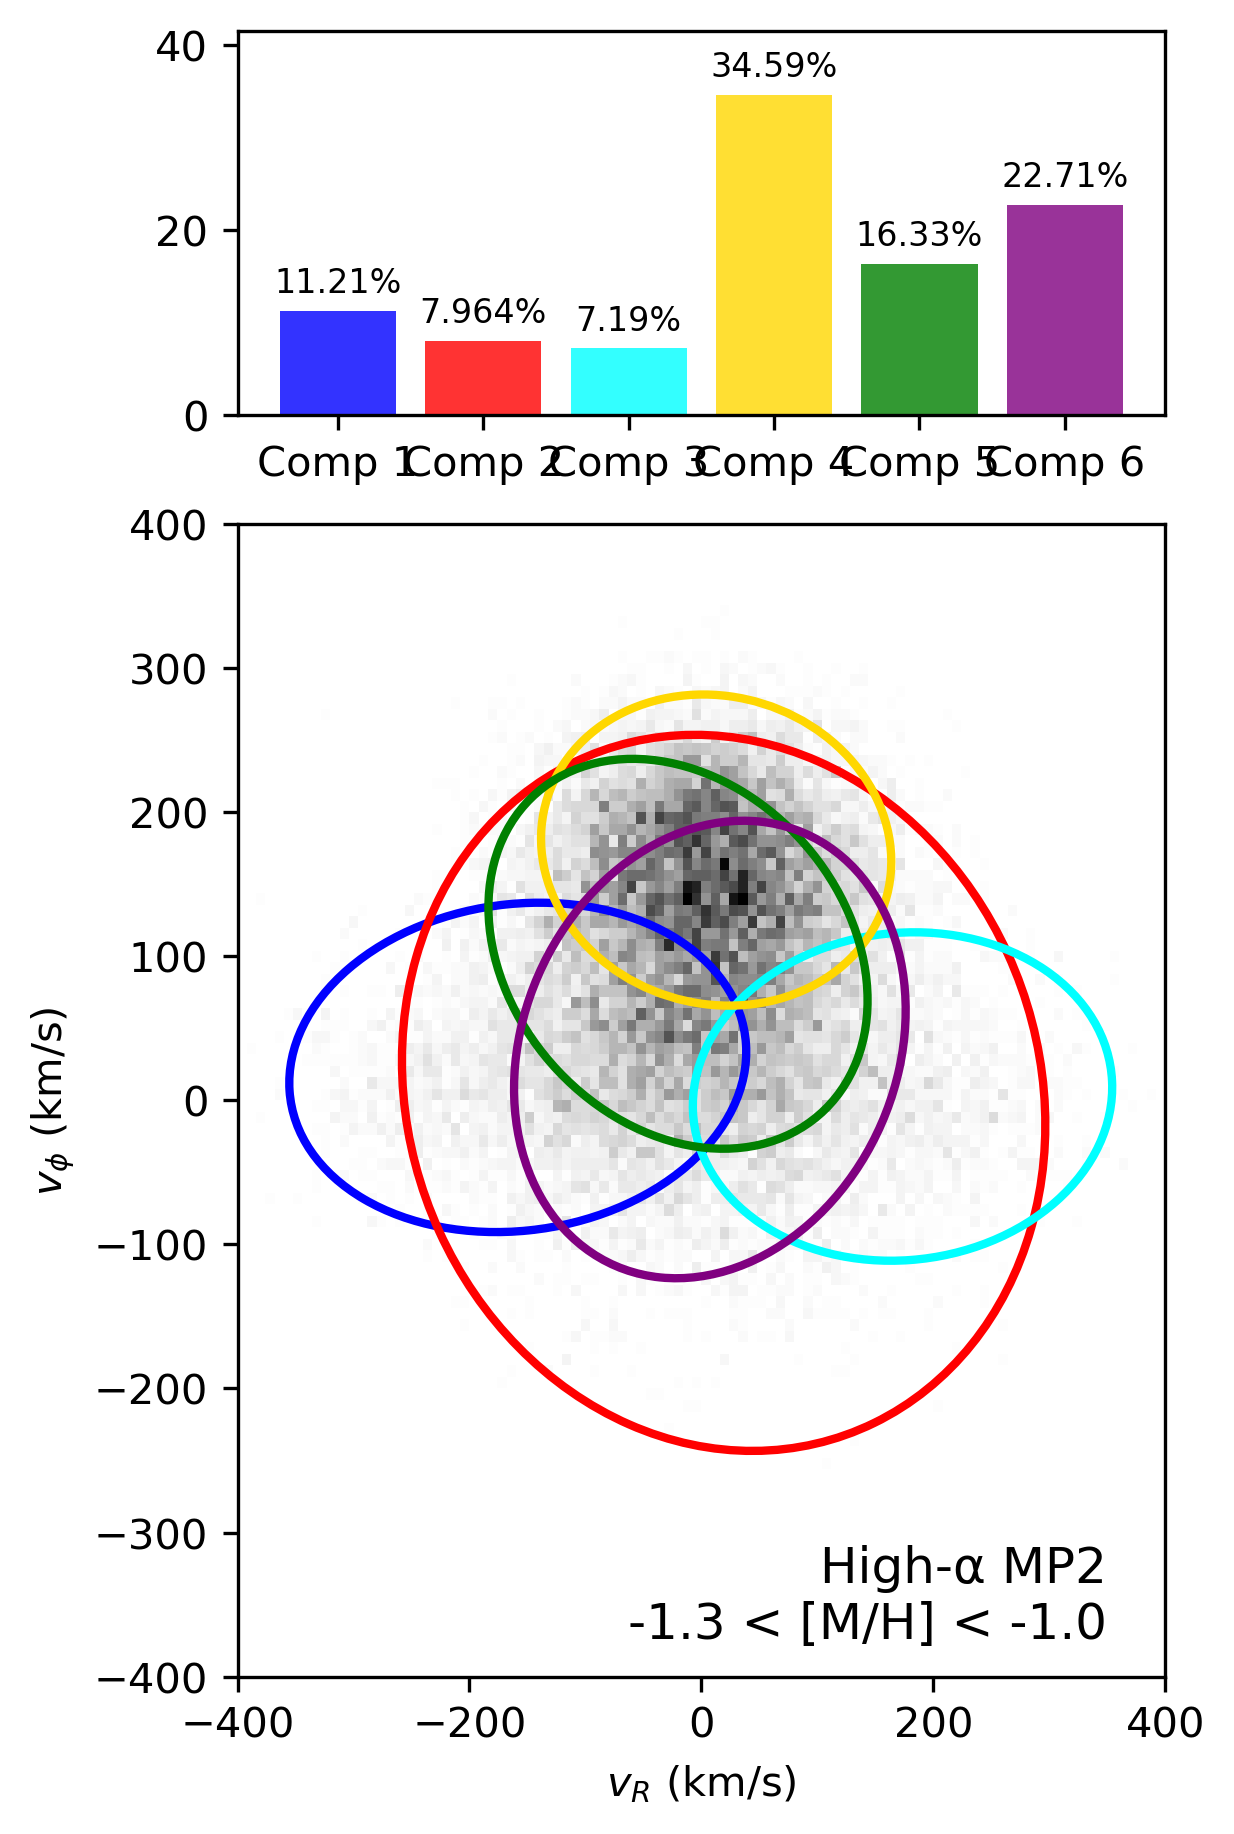
\includegraphics[width=\linewidth]{../figures/gmm_mp2_high_alpha_k6.png}
    \caption{\href{https://raw.githack.com/raunaq-rai/Disentangling-the-Milky-Way-using-GMM/main/figures/MP2\_high\_\_\_-1.3\%5BM\_H\%5D-1.0.html}{MP2}}
    \label{fig:mp2_hi}
  \end{subfigure}

  \caption{XD–GMM decomposition of high-$\alpha$ giants in four metallicity bins. Grey ellipses mark the $1\sigma$ contours of each Gaussian component; click the subcaptions to open the interactive 3D plots.}
  \label{fig:gmm_4wide_hi}
\end{figure}





\begin{table}[H]
\centering
\begin{tabular}{lccccccc}
\hline
\textbf{Components} & \textbf{Weights (\%)} & $\mathbf{v_R}$ & $\boldsymbol{\sigma_R}$ & $\mathbf{v_\phi}$ & $\boldsymbol{\sigma_\phi}$ & $\mathbf{v_Z}$ & $\boldsymbol{\sigma_Z}$ \\
\hline
\multicolumn{8}{l}{\textbf{VMP:} $-3.0 < \mathrm{[M/H]} < -2.0$ (657 stars)} \\
Stationary halo     & 100.0 &   1.40 & 137.36 &  35.59 & 111.99 &  7.60 & 102.48 \\
\hline
\multicolumn{8}{l}{\textbf{IMP:} $-2.0 < \mathrm{[M/H]} < -1.6$ (5219 stars)} \\
Stationary halo     &  16.7 & -22.06 & 116.74 &  -8.55 & 135.74 & -2.64 & 125.40 \\
Prograde halo       &  51.9 &  10.84 &  90.56 &  84.51 &  94.79 & -0.76 &  69.42 \\
GS/E (1)            &  16.8 &-171.35 &  92.33 &  29.12 &  75.23 &  0.50 &  87.09 \\
GS/E (2)            &  14.5 & 180.48 &  91.48 &  -5.47 &  89.66 & -2.87 &  94.37 \\
\hline
\multicolumn{8}{l}{\textbf{MP1:} $-1.6 < \mathrm{[M/H]} < -1.3$ (10265 stars)} \\
Stationary halo     &   13.7 &   7.44 & 145.24 &  15.90 & 130.80 & -8.97 & 127.11 \\
Prograde halo       &   41.8 &  -5.85 & 120.77 &  20.31 &  89.59 & -1.29 &  72.85 \\
GS/E (1)            &   7.6 &-230.09 &  75.81 &   4.65 &  52.41 &  8.69 &  94.68 \\
GS/E (2)            &   5.7 & 237.61 &  70.43 &  -1.23 &  45.51 & -3.73 &  92.81 \\
Thick disc          &   31.2 &   9.18 &  80.79 & 148.23 &  62.97 &  2.99 &  68.92 \\
\hline
\multicolumn{8}{l}{\textbf{MP2:} $-1.3 < \mathrm{[M/H]} < -1.0$ (17314 stars)} \\
Stationary halo     &  17.7 &  15.91 & 141.96 &   2.13 & 101.75 & -1.68 &  98.90 \\
GS/E                &  30.5 & -18.50 & 141.08 &  22.42 &  56.55 & -2.40 &  77.98 \\
Thick Disk          &  51.8 &   5.22 &  76.27 & 159.54 &  57.94 & -0.83 &  67.18 \\
\hline
\end{tabular}
\caption{GMM component weights and kinematics for the high-$\alpha$ sequence.  
Velocities are in km\,s$^{-1}$. Weights indicate the fraction of stars per metallicity bin.}
\label{tab:gmm_higha_stats}
\end{table}


\subsection{Low alpha Gaussian Mixture Model Fit}

\begin{figure}[H]
  \centering
  \begin{subfigure}{0.24\linewidth}
    \centering
    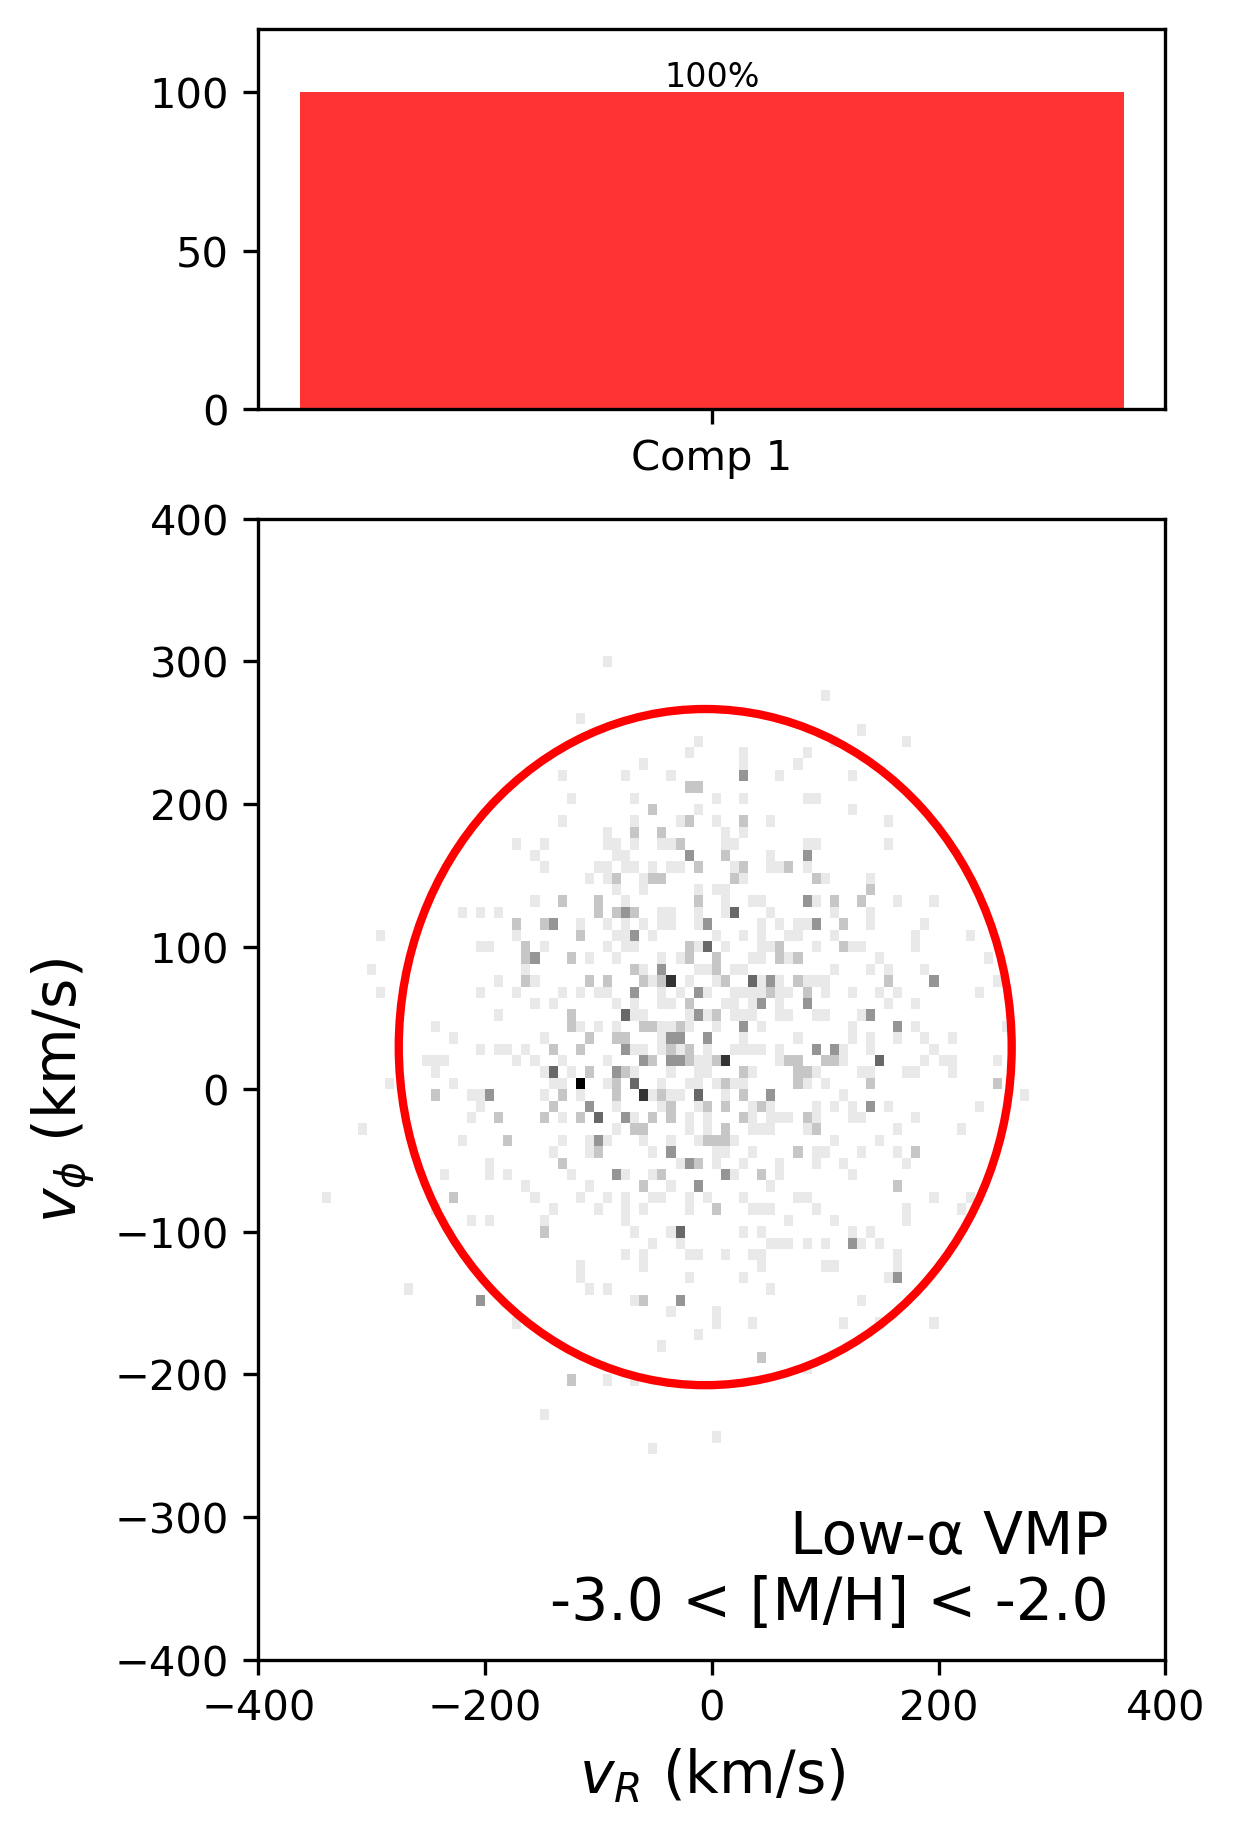
\includegraphics[width=\linewidth]{../figures/gmm_vmp_low_alpha_k1.png}
    \caption{\href{https://raw.githack.com/raunaq-rai/Disentangling-the-Milky-Way-using-GMM/main/figures/VMP_low____-3\%5BM_H\%5D-2.html}{VMP}}
    \label{fig:gmm_vmp_lo}
  \end{subfigure}\hfill
  \begin{subfigure}{0.24\linewidth}
    \centering
    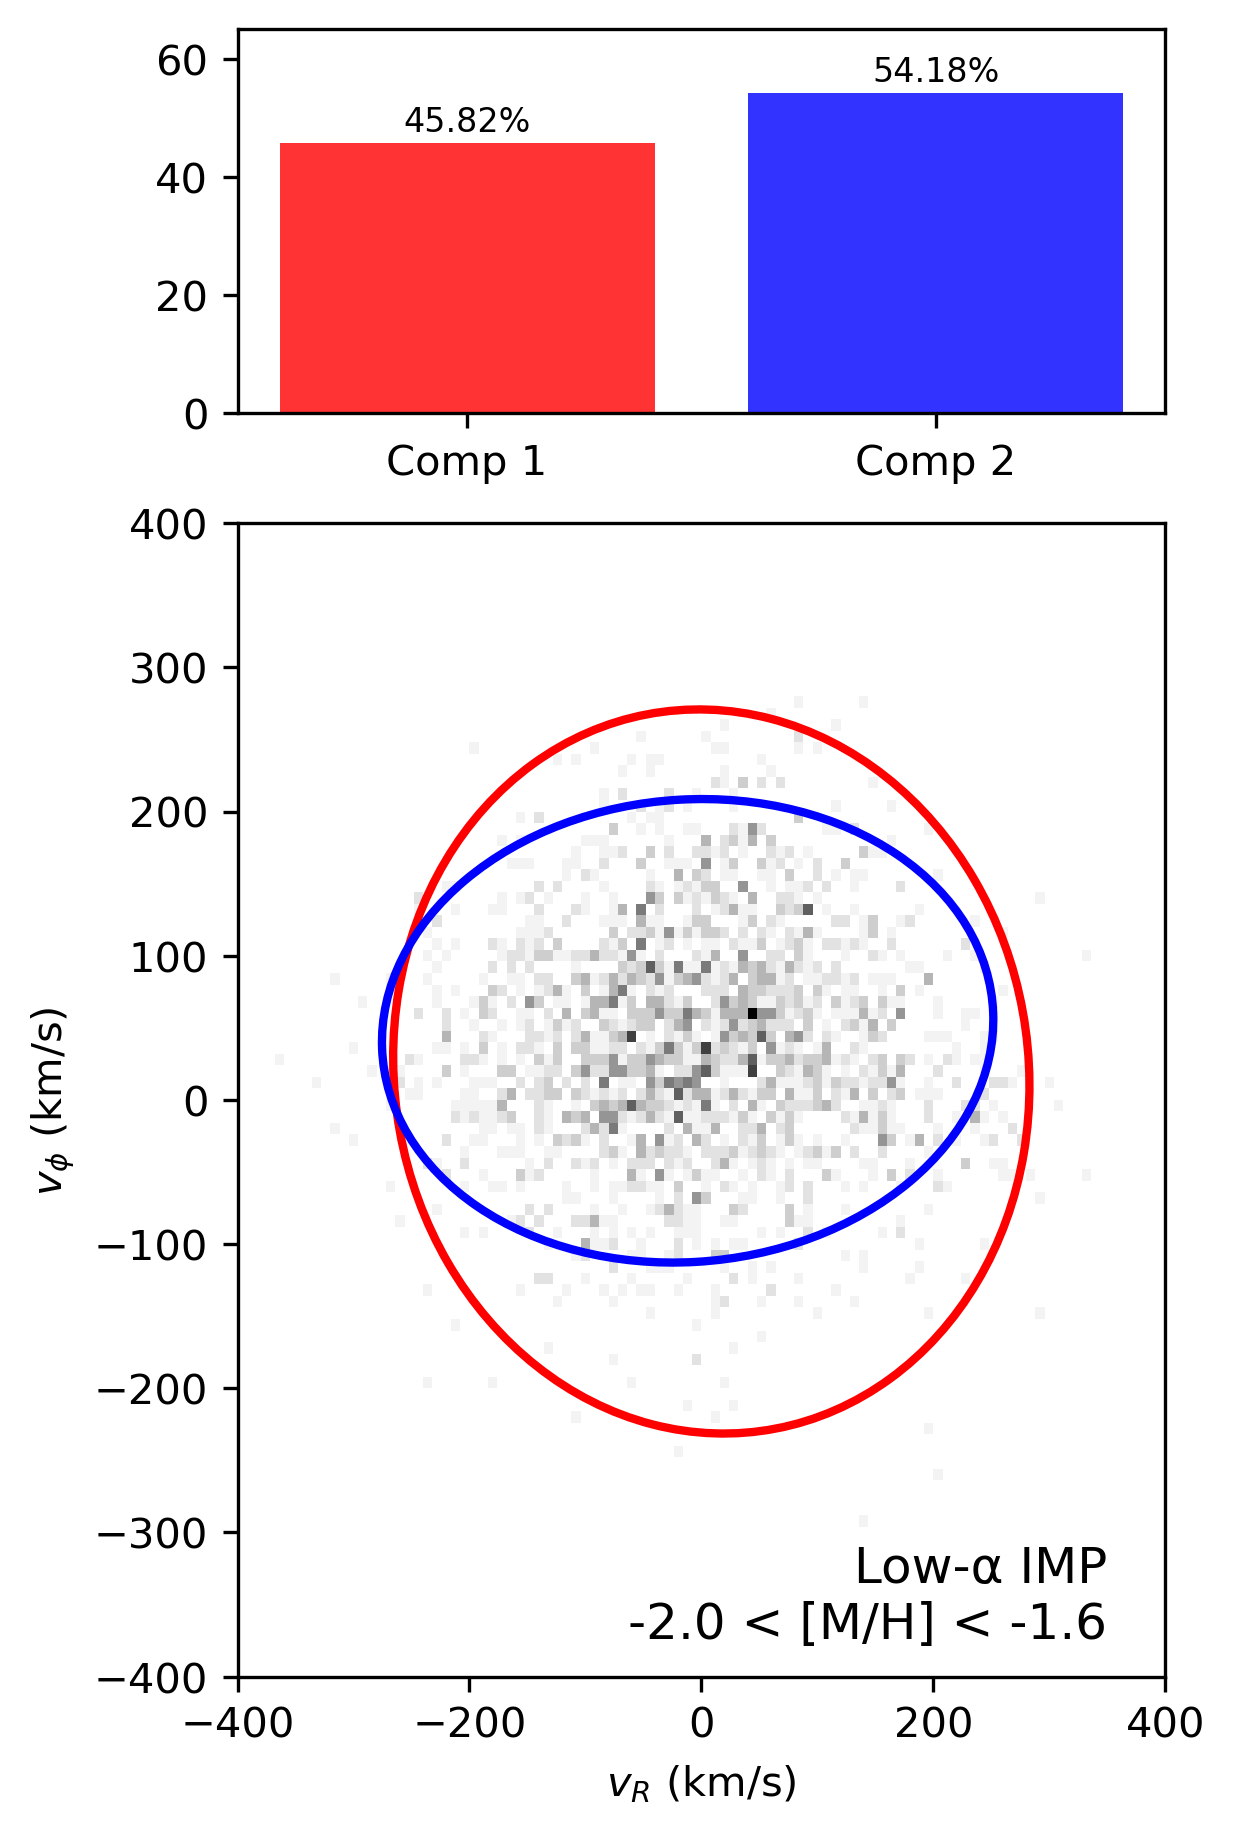
\includegraphics[width=\linewidth]{../figures/gmm_imp_low_alpha_k2.png}
    \caption{\href{https://raw.githack.com/raunaq-rai/Disentangling-the-Milky-Way-using-GMM/main/figures/IMP_low____-2\%5BM_H\%5D-1.6.html}{IMP}}
    \label{fig:gmm_imp_lo}
  \end{subfigure}\hfill
  \begin{subfigure}{0.24\linewidth}
    \centering
    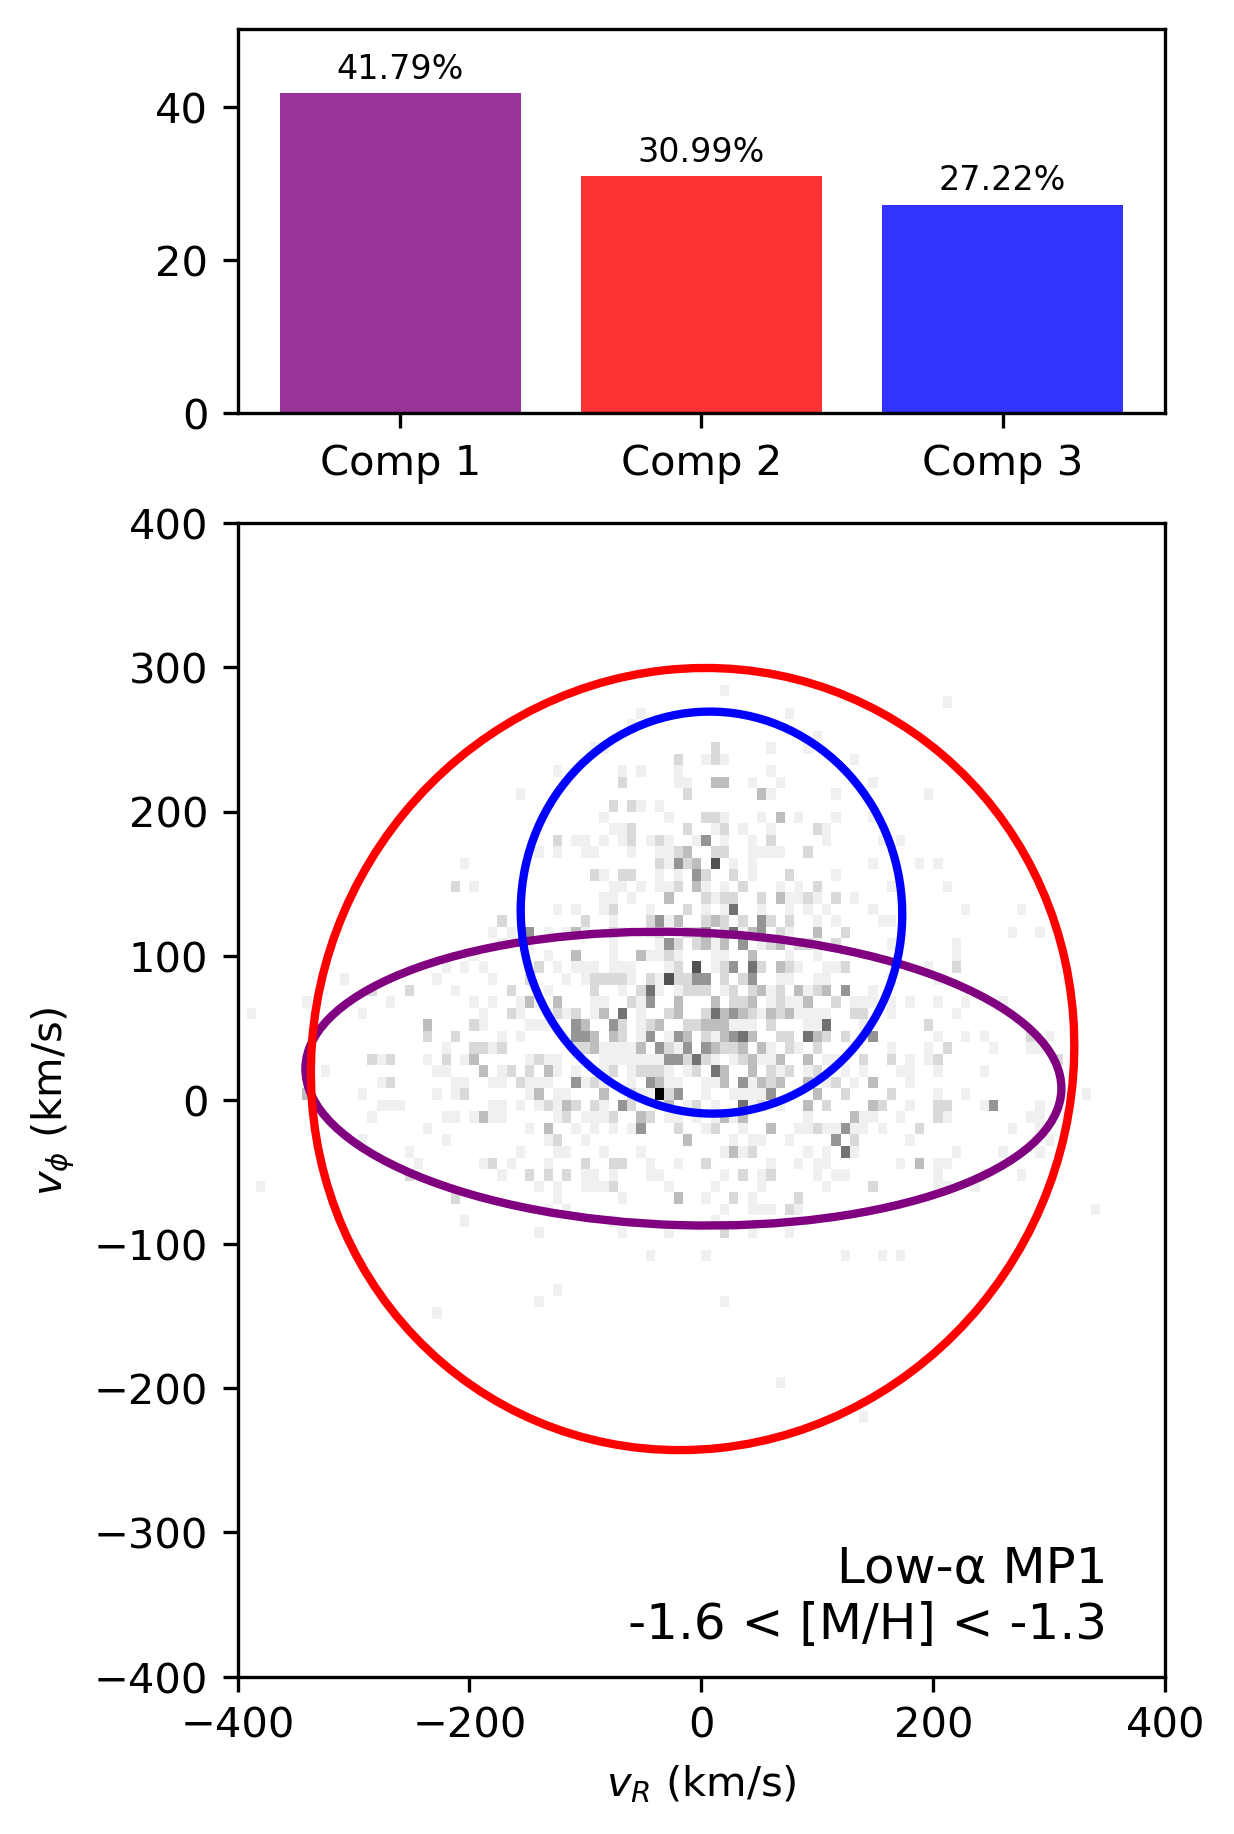
\includegraphics[width=\linewidth]{../figures/gmm_mp1_low_alpha_k4.png}
    \caption{\href{https://raw.githack.com/raunaq-rai/Disentangling-the-Milky-Way-using-GMM/main/figures/MP1_low____-1.6\%5BM_H\%5D-1.3.html}{MP1}}
    \label{fig:gmm_mp1_lo}
  \end{subfigure}\hfill
  \begin{subfigure}{0.24\linewidth}
    \centering
    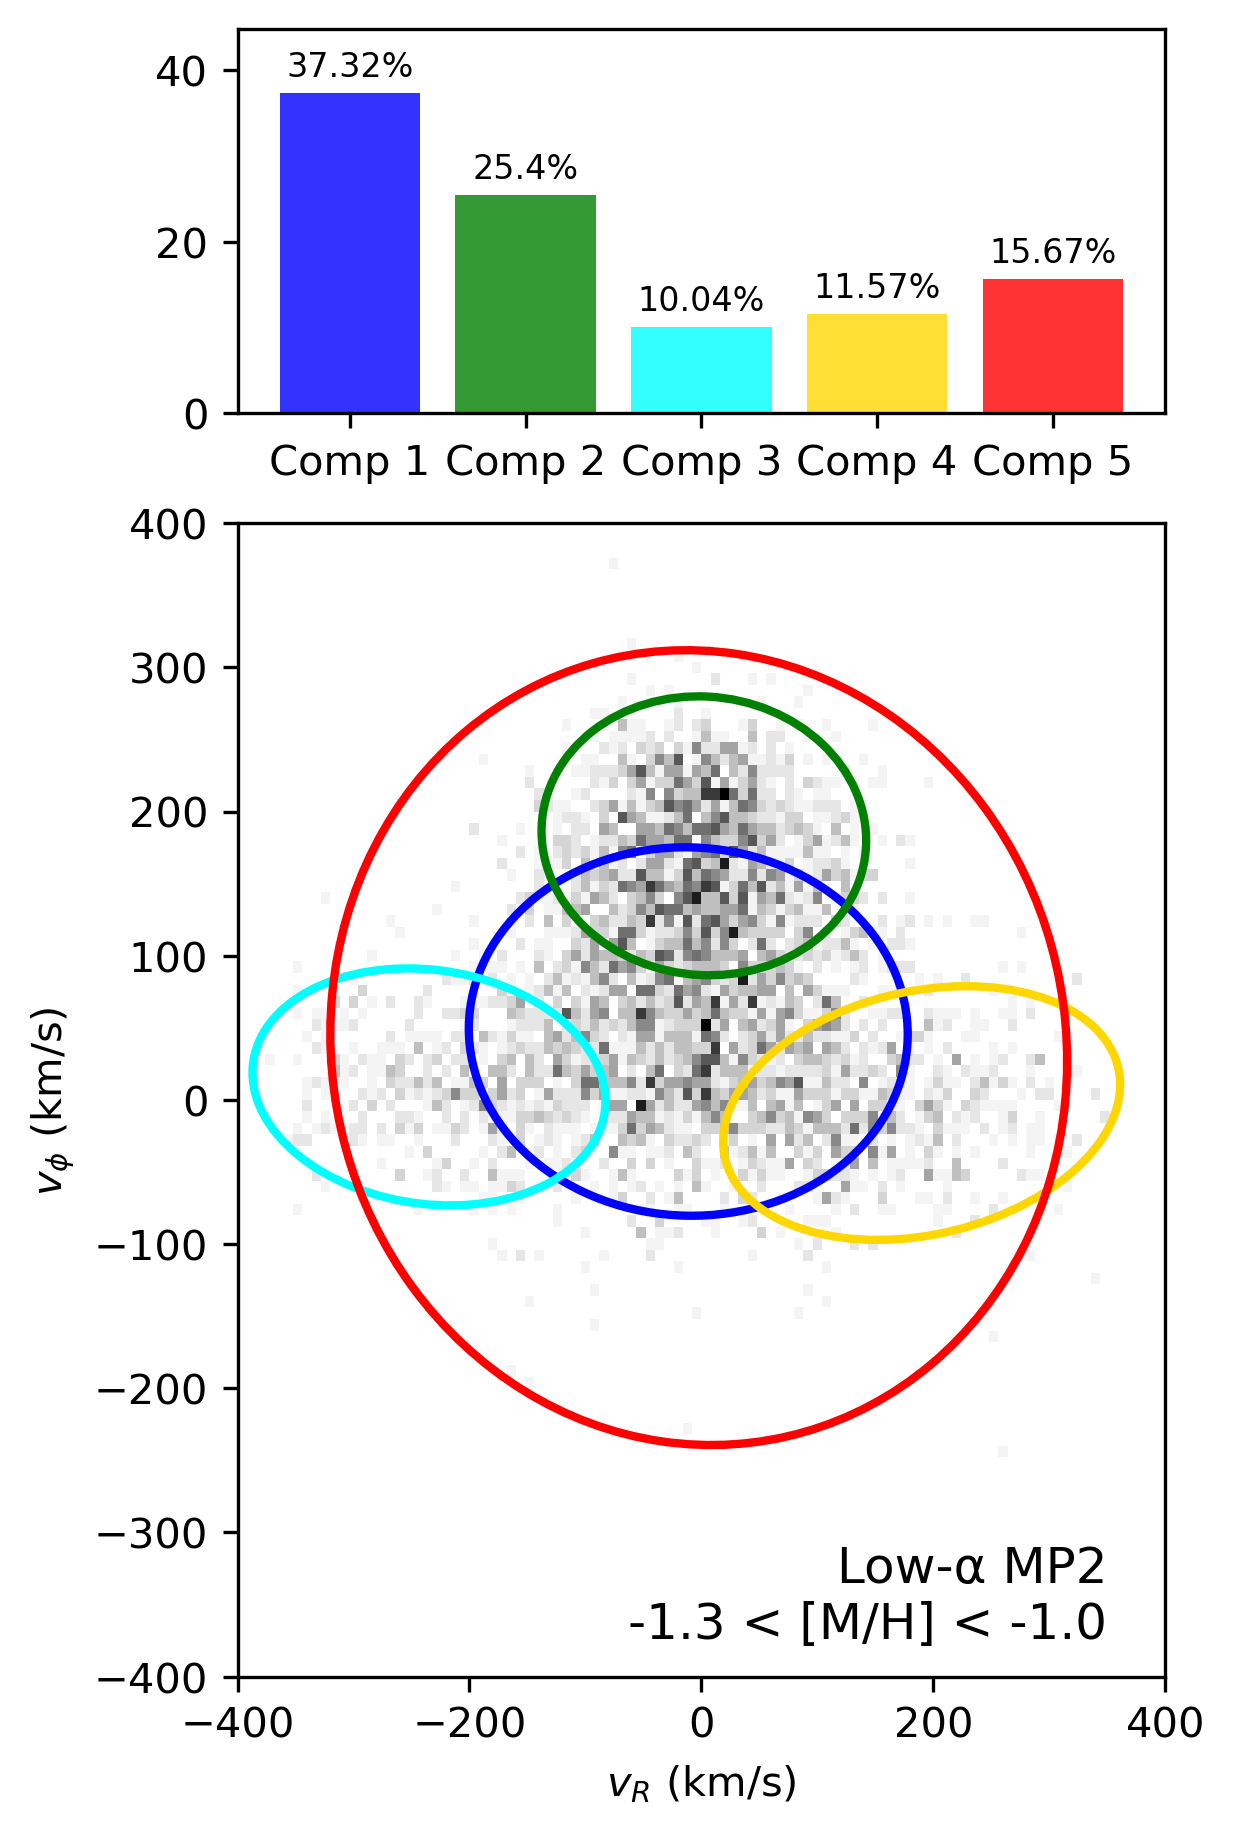
\includegraphics[width=\linewidth]{../figures/gmm_mp2_low_alpha_k6.png}
    \caption{\href{https://raw.githack.com/raunaq-rai/Disentangling-the-Milky-Way-using-GMM/main/figures/MP2_low____-1.3\%5BM_H\%5D-1.0.html}{MP2}}
    \label{fig:gmm_mp2_lo}
  \end{subfigure}

  \caption{XD–GMM decomposition of low-$\alpha$ giants in four metallicity
           bins.  Grey ellipses show the $1\sigma$ contours of every Gaussian component; click the subcaptions to open the interactive 3D plots.}
  \label{fig:gmm_lowalpha_panel}
\end{figure}


\begin{table}[H]
\centering
\begin{tabular}{lccccccc}
\hline
\textbf{Components} & \textbf{Weights (\%)} & $\mathbf{v_R}$ & $\boldsymbol{\sigma_R}$ & $\mathbf{v_\phi}$ & $\boldsymbol{\sigma_\phi}$ & $\mathbf{v_Z}$ & $\boldsymbol{\sigma_Z}$ \\
\hline
\multicolumn{8}{l}{\textbf{VMP:} $-3.0 < \mathrm{[M/H]} < -2.0$ (2929 stars)} \\
Stationary halo     & 100.0 &  -5.82 & 135.18 &  29.55 & 118.56 &  1.34 & 107.10 \\
\hline
\multicolumn{8}{l}{\textbf{IMP:} $-2.0 < \mathrm{[M/H]} < -1.6$ (3228 stars)} \\
Stationary halo     &  37.1 &  12.33 & 139.85 &  22.87 & 129.23 & -4.43 & 120.51 \\
Prograde halo       &  62.9 &  -7.34 & 138.11 &  49.68 &  91.25 &  4.08 &  75.99 \\
\hline
\multicolumn{8}{l}{\textbf{MP1:} $-1.6 < \mathrm{[M/H]} < -1.3$ (3603 stars)} \\
Stationary halo     &  31.0 &  -7.58 & 164.57 &  28.31 & 135.62 & -4.92 & 121.66 \\
GS/E                &  41.8 & -15.50 & 162.97 &  14.71 &  50.94 & -1.93 &  73.60 \\
Thick Disk/prograde halo   &  27.2 &   8.72 &  82.25 & 129.87 &  69.71 &  3.13 &  60.68 \\
\hline
\multicolumn{8}{l}{\textbf{MP2:} $-1.3 < \mathrm{[M/H]} < -1.0$ (7945 stars)} \\
Stationary halo     &  15.7 &  -2.30 & 158.84 &  36.24 & 137.81 &  2.81 & 131.10 \\
Prograde halo       &  37.3 & -11.31 &  94.62 &  47.39 &  63.89 & -1.18 &  63.12 \\
GS/E (1)            &  10.0 &-234.89 &  76.09 &   8.99 &  41.09 & 10.70 &  93.79 \\
GS/E (2)            &  11.6 & 189.95 &  85.58 &  -9.15 &  43.99 & -8.49 &  89.69 \\
Thick disc          &  25.4 &   2.13 &  69.98 & 183.15 &  48.36 &  1.75 &  54.21 \\
\hline
\end{tabular}
\caption{XD--GMM component weights and kinematics for the low-$\alpha$ sequence.  
         Velocities are in km\,s$^{-1}$. Weights are the fractional contribution of each component.}
\label{tab:gmm_lowa_stats}
\end{table}



\subsection{\texorpdfstring{Contrasting the high and low $\alpha$ GMMs}{Contrasting the high/low–alpha GMMs}}
\label{subsec:gmm_comparison}

\begin{figure}[H]
  \centering
  \begin{subfigure}{0.48\linewidth}
    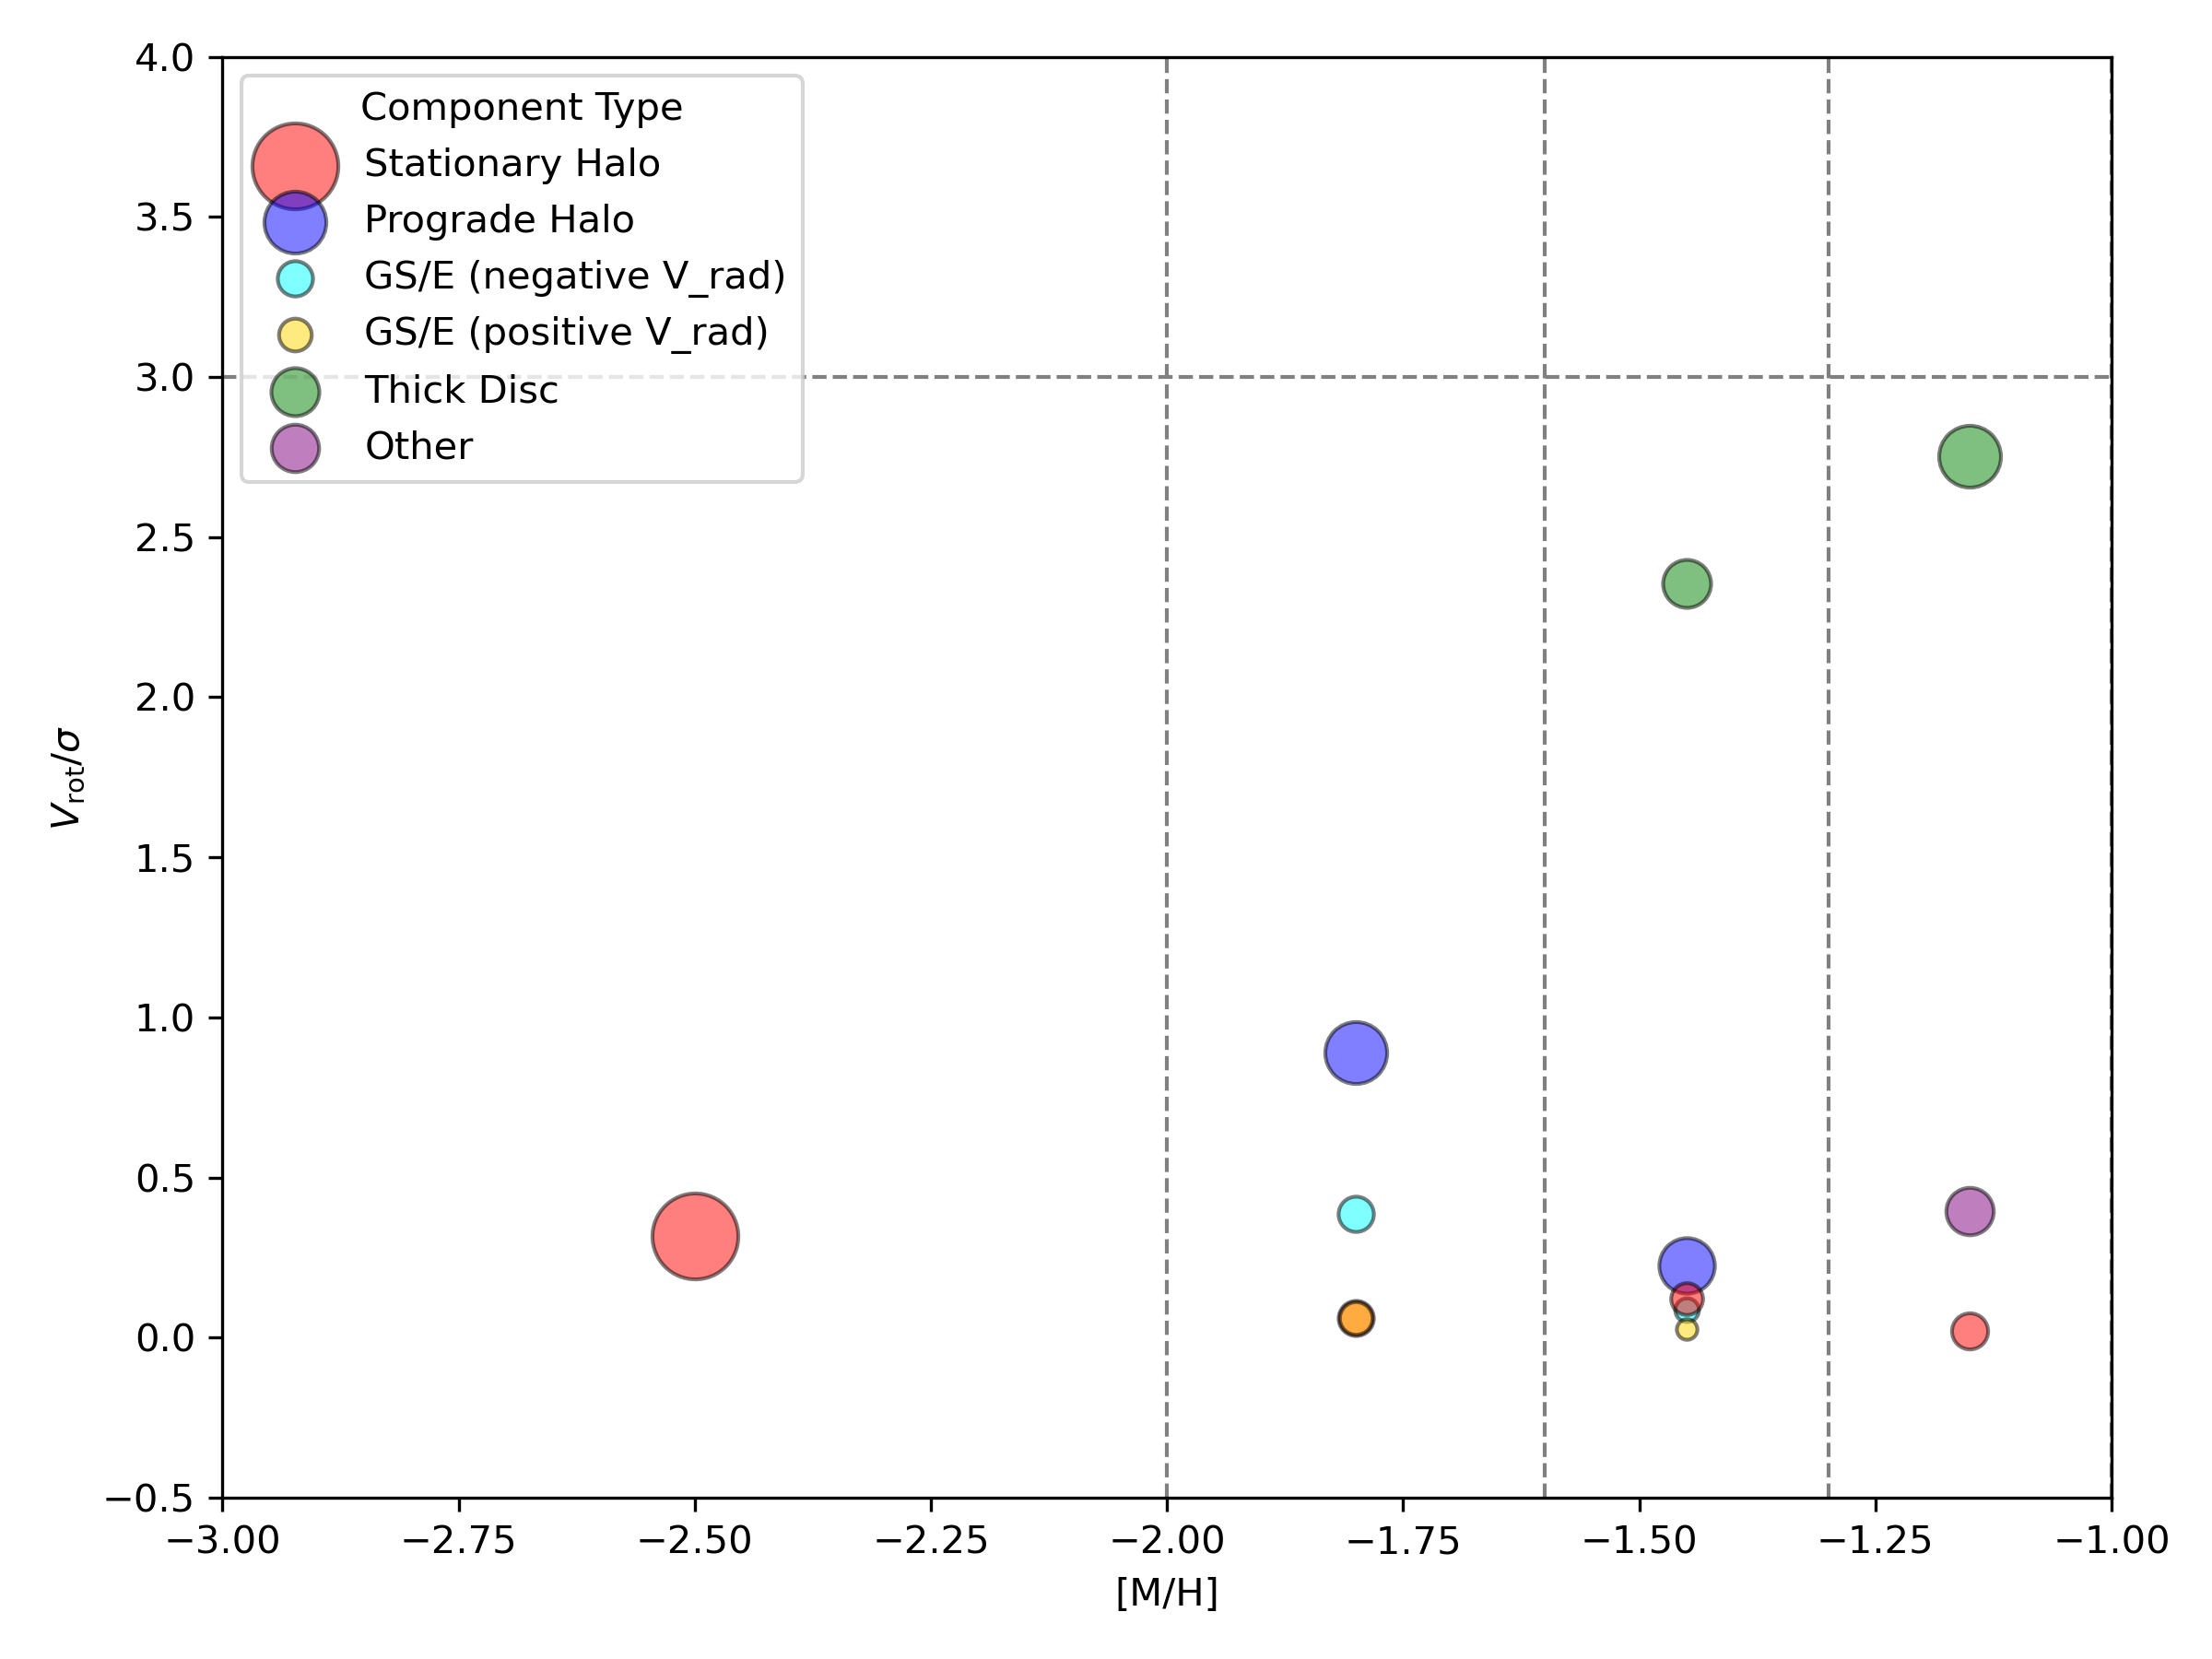
\includegraphics[width=\linewidth]{../figures/v_over_sigma_per_component_highalpha.png}
    \caption{High-$\alpha$ sequence}
    \label{fig:v_over_sigma_high}
  \end{subfigure}
  \hfill
  \begin{subfigure}{0.48\linewidth}
    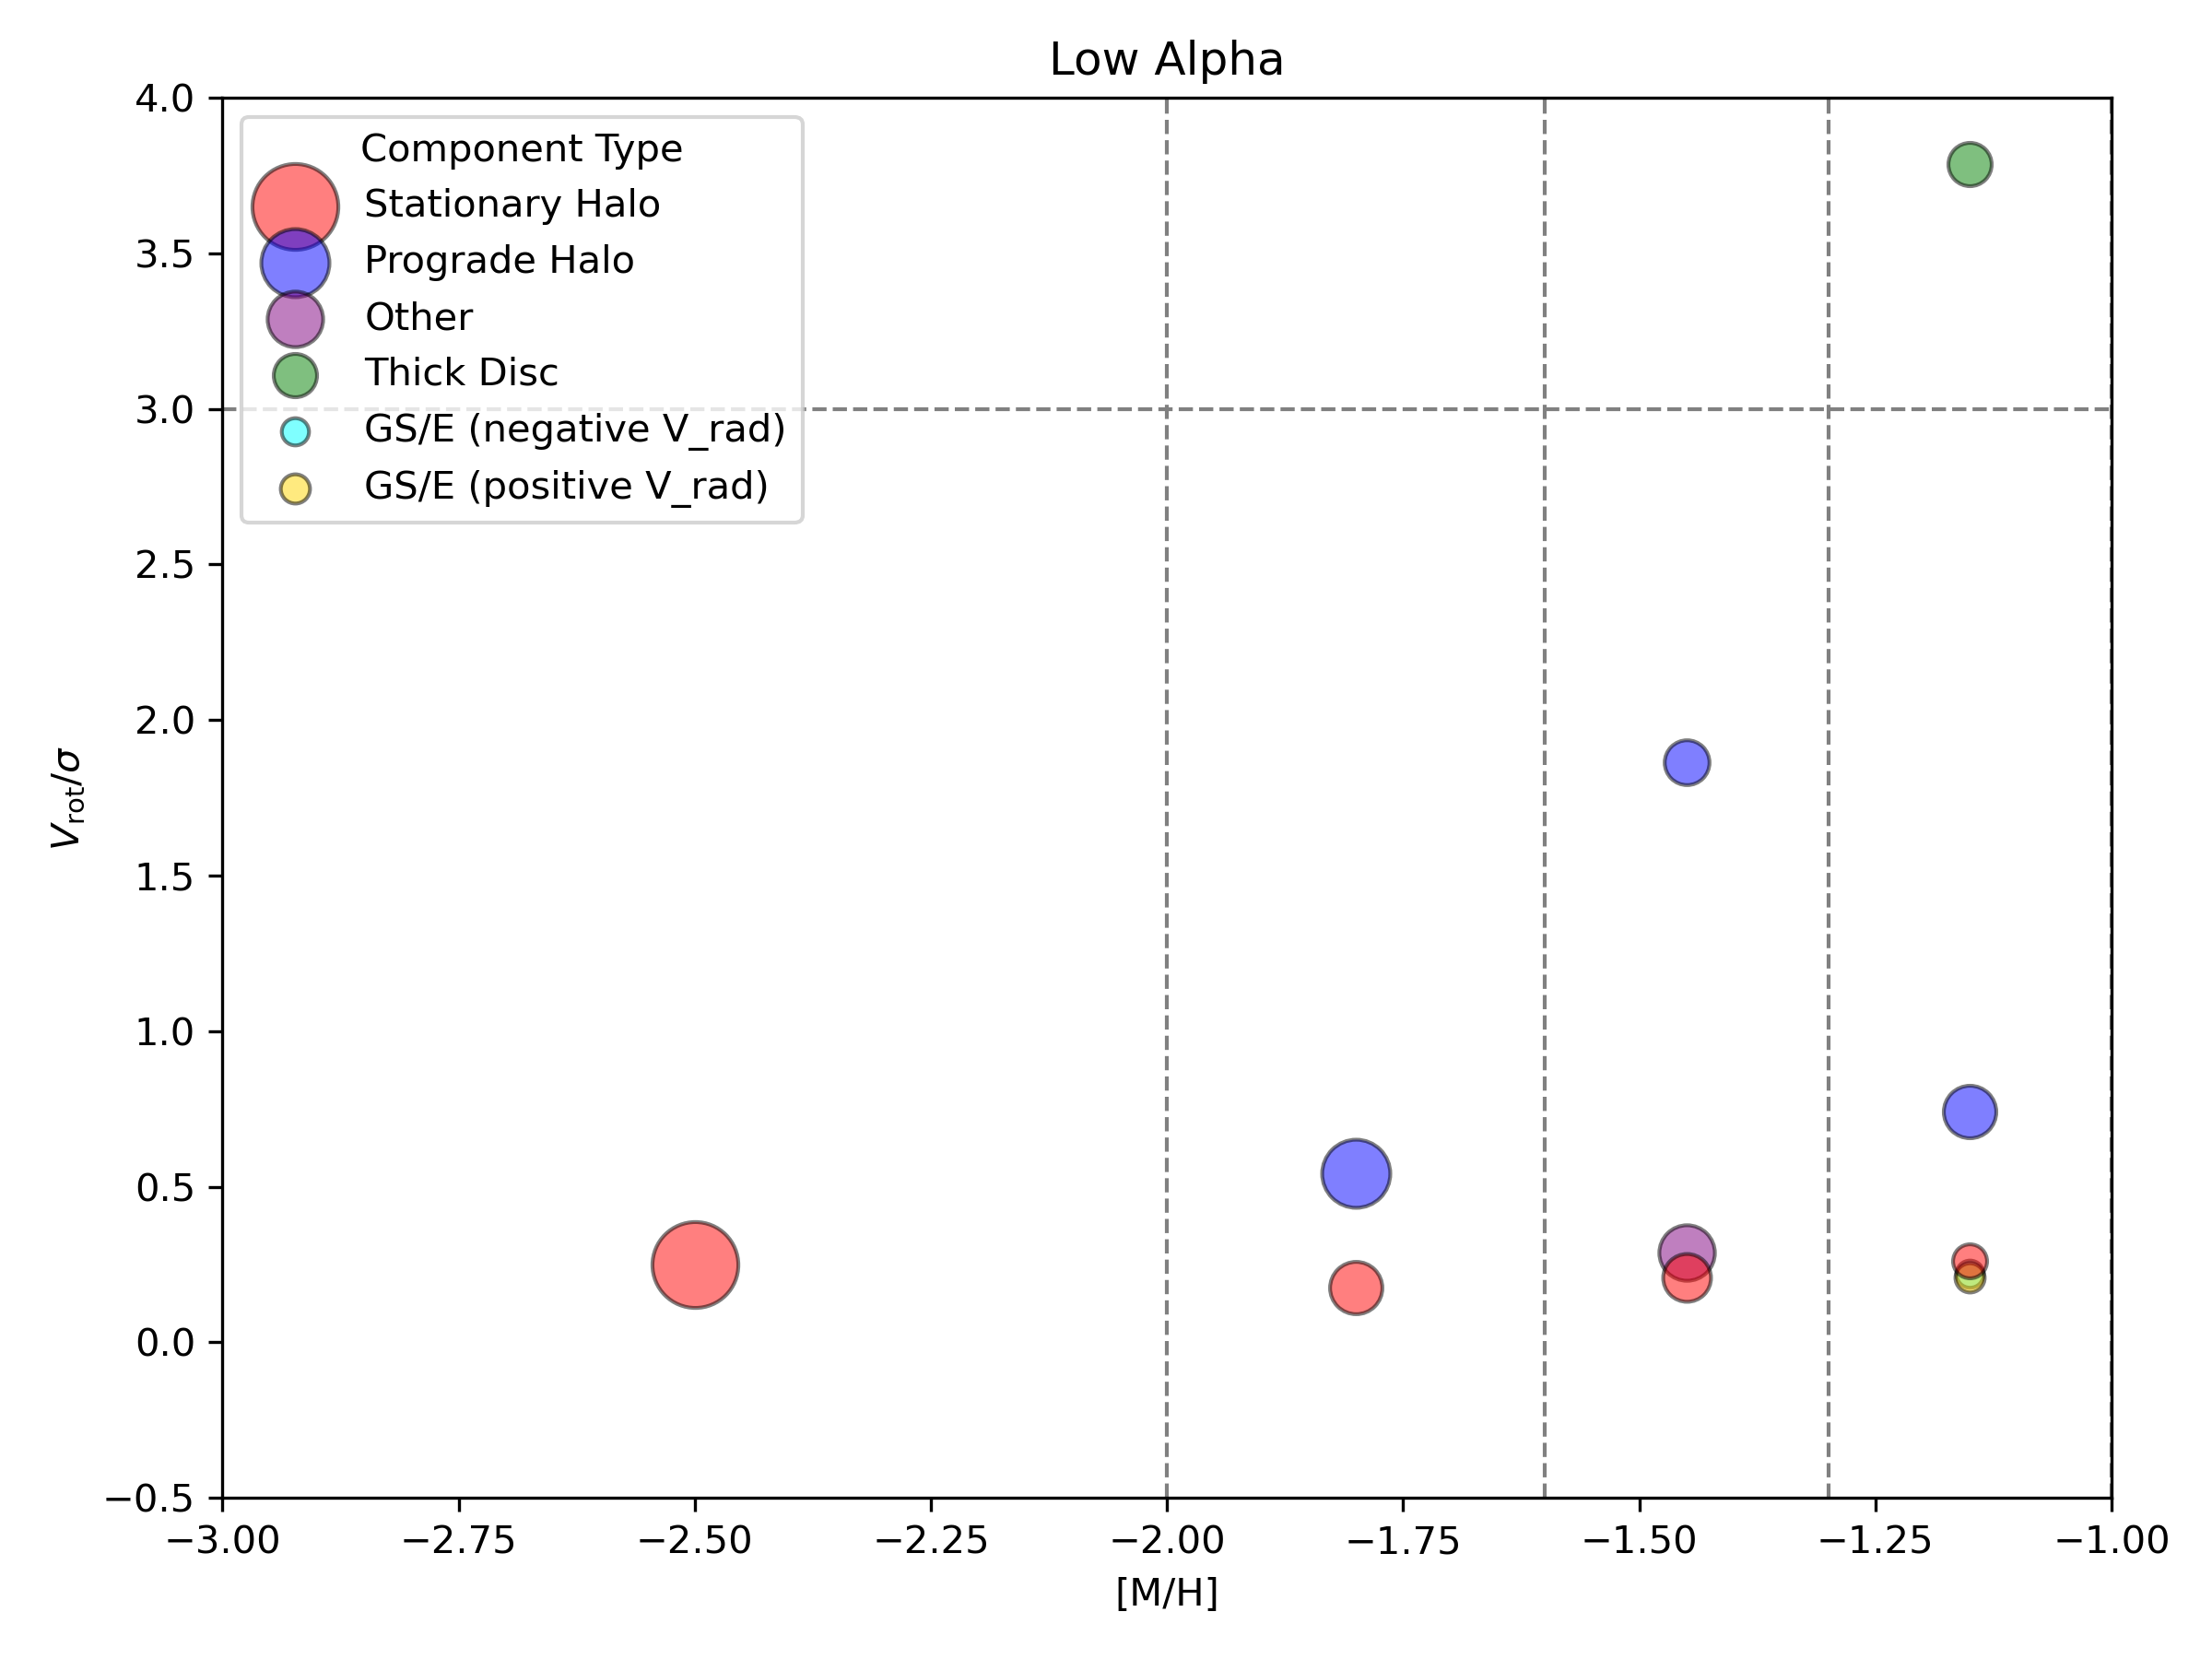
\includegraphics[width=\linewidth]{../figures/v_over_sigma_per_component_lowalpha.png}
    \caption{Low-$\alpha$ sequence}
    \label{fig:v_over_sigma_low}
  \end{subfigure}

  \caption{Ratio of the mean rotational velocity to azimuthal velocity dispersion, $V_{\rm rot}/\sigma_\phi$, for individual GMM components in each metallicity bin. Larger circles represent more dominant components. Colours correspond to those in Figures~\ref{fig:gmm_4wide_hi} and \ref{fig:gmm_lowalpha_panel}. This is created in the same way as Figure~\ref{fig:v_over_sigma}.}
  \label{fig:v_over_sigma_alpha}
\end{figure}

In the very-metal-poor bin (VMP; $[\mathrm{M/H}] < -2$), both high- and low-$\alpha$ populations are dominated by a single, isotropic, non-rotating halo component. The similarity in $V_{\rm rot}/\sigma_\phi$ across both tracks implies that $\alpha$-abundance has little influence on halo structure at these low metallicities.

At intermediate metallicities (IMP; $-2.0 < [\mathrm{M/H}] < -1.6$), the low-$\alpha$ sample separates into stationary and prograde halo components, while the high-$\alpha$ fit includes two radially biased components with limited rotation. These are likely artefacts of overfitting or contamination by misclassified low-$\alpha$ stars.

In the MP1 bin ($-1.6 < [\mathrm{M/H}] < -1.3$), a thick disc component emerges in the high-$\alpha$ population, showing moderate $V_{\rm rot}/\sigma_\phi$, indicative of in-situ disc formation. Meanwhile, the low-$\alpha$ population develops a GSE-like halo structure, supporting a scenario where the GSE merger occurred around the onset of high-$\alpha$ disc formation \citep{Helmi2018}.

In the most metal-rich bin (MP2; $-1.3 < [\mathrm{M/H}] < -1.0$), both sequences display prominent disc components. The high-$\alpha$ disc is kinematically hotter and more massive, while the low-$\alpha$ disc shows a sharp increase in $V_{\rm rot}/\sigma_\phi$, consistent with a dynamically colder, thin-disc-like population. The abrupt rise suggests that thin disc formation may have occurred rapidly in the low-$\alpha$ sequence, in contrast to the more gradual buildup in the high-$\alpha$ case. The absence of an ultra-cold thin disc in either track reflects a selection bias against stars near the Galactic plane.


%------------------------------------------------------------------
\section{Discussion} \label{sec:discussion}

The discussion of the GMM process mirrors that of the discussion in \citet{zhang2024existencemetalpoordiscmilky}.
Since the primary goal of this report was to assess the reproducability of \citet{zhang2024existencemetalpoordiscmilky},
the discussion will focus on the differences between the results of this report and those of \citet{zhang2024existencemetalpoordiscmilky}.
We do however mention the limitations of the GMM approach and selection effects - which are largely 
the same as those discussed in \citet{zhang2024existencemetalpoordiscmilky}.

\subsection{\texorpdfstring{Reproducability of \citet{zhang2024existencemetalpoordiscmilky}}{Reproducability of Zhang et al.\ (2024)}}


The GMM decomposition presented in this report successfully reproduces the same structural features reported 
by \citet{zhang2024existencemetalpoordiscmilky} by selecting the minimum BIC score for each bin. However, there 
are several differences in our results worth highlighting.

At the very metal-poor end, our model recovers a nearly even split between stationary and prograde halo 
components, in contrast to the more dominant non-rotating halo found by \citet{zhang2024existencemetalpoordiscmilky}. 
Although the underlying stellar samples are largely the same, this discrepancy likely reflects the 
sensitivity of the GMM to initialisation and the precise kinematic distribution of stars in this 
low-metallicity regime, where substructure is subtle and overlapping. Notably, the kinematics of the 
prograde component in our fit are consistent with those reported for Aurora \citep{Belokurov2022}, 
suggesting it may correspond to an early, slightly rotating in-situ population.

In the intermediate metallicity regime ($-2.0 < \mathrm{[M/H]} < -1.6$), both studies show GSE-like 
signatures. The agreement in component structure is remarkably consistent, though our fit assigns slightly 
more weight to the GSE substructures. Interestingly, our GSE components appear with clearer symmetry in radial 
velocity, which may indicate differences in how the GMM partitions stars with highly eccentric orbits. 
The recovery of these features in both analyses suggests an ancient radial merger consistent with GS/E \citep{Belokurov2020}.

In the disc onset bin ($-1.6 < \mathrm{[M/H]} < -1.3$), we find a somewhat higher fraction of 
thick-disc stars than \citet{zhang2024existencemetalpoordiscmilky}, along with slightly lower rotational 
velocities. This could be due to small variations in how the GMM distinguishes between disc-like and 
halo-like stars in the transition regime. Despite this, both studies detect a clear emergence of a warm, 
rotating in-situ component, consistent with the kinematics of a thick disk.

By $[\mathrm{M/H}] > -1.3$, the thick disc becomes a dominant structure in our analysis and that performed
by \citet{zhang2024existencemetalpoordiscmilky}, almost surpassing the weight of the prograde halo.

In summary, while small discrepancies exist, particularly in the balance between halo and prograde components 
at low metallicity, there is an overall agreement in results.

We note that we do not attempt to reproduce the action-space analysis of \citet{zhang2024existencemetalpoordiscmilky} in this report. 
This decision reflects the fact that our analysis focuses on the use of the XD-GMM algorithm, and because of our
understanding that orbital actions do not generally follow Gaussian distributions. Unlike velocity space, which can often be 
approximated as locally Gaussian for distinct stellar populations, action space retains strong imprints 
of past dynamical processes (e.g. mergers, phase-mixing, resonances) that result in highly non-Gaussian, 
often multimodal structures.



\subsection{\texorpdfstring{Expansion of \citet{Vis2024}}{Expansion of Viswanathan et al.\ (2024)}}


We extended the XD-GMM analysis to the high and low $\alpha$ sequences identified by \citet{Vis2024}. 
Rather than assuming two Gaussian components as in \citet{Vis2024}, we fit a
Gaussian mixture model with varying numbers of components in each metallicity bin for both sequences. 
For each case, the optimal number of components was selected based on the minimum BIC score.
This allows us to capture the full complexity of the kinematic structure in both sequences,
including the presence of multiple halo components and the emergence of thick disc structures 
at different metallicities.

We were successfully able to reproduce the figures and data preparation described in \citet{Vis2024}, as shown in the plots of 
Section~\ref{subsec:data_vis}.

As outlined in Section~\ref{subsec:alpha}, we expected structural differences between the high- and low-$\alpha$ sequences 
to emerge in the GMM fits. These expectations were largely met: the high-$\alpha$ stars exhibited a clear transition 
towards a rotationally supported disc at earlier metallicities, while the low-$\alpha$ stars remained halo-dominated 
until higher metallicities.

One of the more unexpected outcomes of this analysis is the identification of GS/E components within the 
high-$\alpha$ sequence, despite the GS/E progenitor being associated with a slow star formation 
history that should result in an $\alpha$-poor population. This is likely due to contamination from 
low signal-to-noise abundance measurements, or challenges in separating overlapping kinematic substructures 
when using GMMs. In future work, it would be helpful to consider how abundance uncertainties, particularly at low 
metallicities, may affect the classification of stars. Additionally, as seen in Figure~\ref{fig:alphametal}, 
there appears to be a number of low-$\alpha$ stars at $[\mathrm{M/H}]\sim-2.5$ with 
[$\alpha$/M]~$\sim$~0.1. It remains unclear whether this population is real or the result of measurement 
uncertainties, and it would benefit from further investigation.


\subsection{Selection Effects} \label{subsec:selection_effects}

This part of the discussion closely follows the treatment of selection effects in 
\citet{zhang2024existencemetalpoordiscmilky}. As in their study, our application of quality cuts, such 
as removing stars with high extinction or low Galactic latitude, and enforcing a strict parallax quality 
threshold, introduces a non-trivial selection function that affects the relative detectability of 
different Galactic components.

In particular, the Galactic latitude cut removes many stars near the disc midplane, where the 
thin disc is most prominent. While relaxing this cut does lead to the identification of a
colder, lower-dispersion disc component in the low-$\alpha$ sequence at higher metallicities, this 
component is not considered in our analysis. Our focus is on characterising the onset of disc like 
kinematics across metallicity in both chemical sequences, rather than describing the well established 
thin disc. Including low latitude stars would bias the sample toward the disc population, introduce 
uncertainties in the metallicity estimates, since Gaia XP abundances are known to be less reliable in 
egions of high extinction, and obscure the halo to disc transition that is central to this investigation.


It is important to note that the component weights derived in this work reflect the properties of our 
selected sample and should not be generalised to the full Galaxy without modelling the underlying 
selection function.


\subsection{Limitations of GMM}

Although this part of the discussion mirrors that of \citet{zhang2024existencemetalpoordiscmilky}, 
it is worth reiterating that the Gaussian mixture model approach has several limitations. 
Gaussian mixtures impose symmetric, ellipsoidal structures in velocity space, 
which is an oversimplification of the true distribution function of Galactic populations. 
For instance, the velocity distribution of the thin disc is considered to be non Gaussian 
due to features such as asymmetric drift \citep{Li2024ass}, while the GS/E debris has been shown to display bimodal 
structure in the radial velocity component \citep{Lancaster2019,Necib2019}. 
In addition, resonant interactions with the Galactic bar may introduce asymmetric and non Gaussian 
features in the velocity distributions \citep[e.g.][]{Dillamore2023}. 

Following \citet{zhang2024existencemetalpoordiscmilky}, we therefore restricted our GMM analysis 
to the range $-3 < \mathrm{[M/H]} < -1$, where the thin disc contribution is minimal. At higher 
metallicities, the GMM attempts to describe the sharp kinematic features of the thin disc using 
multiple Gaussians, which are not physically meaningful. While more flexible models based on 
physically motivated distribution functions could better capture these complexities 
\citep[e.g.][]{Binney2010}, they require significantly more computational effort and are 
beyond the scope of the aims of both this report and that of \citet{zhang2024existencemetalpoordiscmilky}.

Another known limitation of GMMs is their reduced sensitivity to small subpopulations. 
Like \citet{zhang2024existencemetalpoordiscmilky}, we find little evidence for a significant 
disc like component at low metallicities, but this absence should be interpreted with caution. 

\subsection{Recommendations and Next Steps}

To sharpen the physical picture exposed by the XD-GMM analysis, the first priority is to
replace descriptive Gaussian mixtures with fully dynamical models.  
Action-based or distribution-function fitting with packages such as \textsc{RoadMapping} or
\textsc{Agama} can recover asymmetric wings and resonant features, tying each kinematic component
directly to the Galactic potential.  
In parallel, cross-matching our \emph{Gaia} sample with high-resolution spectra from APOGEE, 
GALAH, and the forthcoming WEAVE and 4MOST surveys will tighten the $\alpha$-abundance 
uncertainties to a few hundredths of a dex, removing the present overlap between the high- 
and low-$\alpha$ tracks. Once those cleaner chemical labels are in place, a forward model of 
Gaia's selection function—encompassing its magnitude limits, colour cuts, and 
sky-coverage completeness—can translate the fitted mixture weights into \textit{unbiased} 
stellar-mass fractions for each kinematic component. Plotting these bias-corrected masses 
against look-back time, or metallicity, produces a star-formation-efficiency 
(SFE) curve: a quantitative record of how efficiently gas was converted into stars in the 
thick and thin discs at every epoch. Because the underlying masses are corrected for 
observational selection effects, this procedure could deliver reliable
SFE curves for both discs, giving a direct benchmark for galaxy-formation models.

With tighter chemical constraints in hand, the empirical [M/H]–$\alpha$ thresholds can be folded 
into Milky-Way zoom simulations such as \textsc{Auriga} and \textsc{FIRE-2}, allowing the thick- 
and thin-disc analogues to be tracked self-consistently through cosmic time and yielding 
synthetic data cubes tailored to forthcoming observatories.  

Near-infrared imaging with \textit{JWST} is the natural next step: red-giant stars—dominant in 
the low-surface-brightness outskirts of spirals—peak in the NIR and are only weakly affected by 
dust.  \textit{JWST} therefore resolves individual giants well beyond the Local Group, and 
NIRSpec simultaneously records the CO, CN and Fe-peak features required for accurate 
\([\mathrm{M/H}]\) and \([\alpha/\mathrm{Fe}]\) measurements for each star \citep{Jakobsen_2022}.

The Rubin Observatory's Legacy Survey of Space and Time will deliver the complementary view.  
A decade of deep, multi-epoch imaging will map whole galactic discs to very faint limits, 
provide sub-mas\,yr\(^{-1}\) proper motions for bright giants, and trace stellar-density 
variations at per-cent fidelity \citep{Ivezic2019}.  Combined, \textit{JWST} spectroscopy 
and LSST astrometry will furnish full six-dimensional phase-space coordinates plus detailed 
chemistry for resolved giants in dozens of nearby spirals.  

Once those data arrive, the XD-GMM method can be applied 
wholesale to external galaxies, decomposing their velocity fields into halo, thick-disc and 
thin-disc components and measuring the metallicity-$\alpha$ spin-up thresholds in each system.  
What is now a single-galaxy case study will become a statistically robust, cross-galaxy 
experiment that tests the Milky Way's two-phase disc-assembly scenario against a much broader 
population of spirals.




\section{Conclusion}

We have successfully reproduced the XD-GMM work of \citet{zhang2024existencemetalpoordiscmilky} with
\textit{Gaia}~DR3 red giants and confirmed that no rotation-supported disc exists below
${\rm [M/H]}\!\simeq\!-2$, while ordered rotation appears at
${\rm [M/H]}\!\simeq\!-1.6$.  Adding XP-based $\alpha$ abundances
\citep{Li2024} and the high/low-$\alpha$ split of \citet{Vis2024} reveals a chemically
tagged, two-phase timeline: high-$\alpha$ stars spin up first and build the thick disc,
whereas low-$\alpha$ stars remain halo-like until ${\rm [M/H]}\!\approx\!-1.3$, signalling
the birth of a less-dispersed disc, signalling thin-disk onset.  These thresholds tighten 
earlier, purely metallicity pictures of disc growth and provide quantitative anchors for 
dynamical modelling, chemical-tagging surveys and simulation work.

The path forward is therefore clear: adopt action-based distribution-function fitting to
replace descriptive Gaussians, sharpen the $\alpha$ scale with forthcoming high-resolution
spectroscopy, correct mixture weights with an explicit \textit{Gaia} selection function,
and inject the resulting [M/H]-$\alpha$ thresholds into \textsc{Auriga} and
\textsc{FIRE-2} zoom simulations.  Synthetic \textit{JWST} and LSST data built from those
simulations will put the Milky Way's two-phase disc-assembly timeline to its first
rigorous, galaxy-to-galaxy test.









\newpage
\bibliographystyle{abbrvnat}
\bibliography{references}

\section*{Declaration of Use of AI Tools}

I declare that all ideas, methods, and approaches used in this project were 
conceived and developed independently through my own research, understanding 
and engagement with lecture and supervision material. The work presented here 
is entirely my own.

The following AI tools were used for support purposes:
\begin{itemize}
    \item \textbf{ChatGPT:} Used to refine code snippets, assist with LaTeX 
    formatting, assist with documentation, and improve the clarity and structure. 
    All content generated by this tool was critically evaluated and adapted.
    \item \textbf{GitHub Copilot:} Used to suggest coding snippets and assist 
    the implementation of functions. All suggested code was reviewed, modified, 
    and tested.
\end{itemize}


\end{document}
